\documentclass[a4paper,12pt,twoside,draft]{book}
\usepackage[tikz,listings]{261216}
\title{Discrete Mathematics for Computer Engineers \\
วิยุตคณิตเพื่อวิศวกรคอมพิวเตอร์}
\author{Chinawat Isradisaikul \\ ชินวัตร อิศราดิสัยกุล}

\makeatletter
\renewcommand\@pnumwidth{2em}
\makeatother

\newcommand\cd[1]{\lstinline{#1}}

\hypersetup{final,linkcolor=blue,linktoc=all}

\usepackage{mathpartir}

\usepackage{rotating}
\newcommand\rotatedhdr[1]{\multicolumn{1}{c}{\begin{rotate}{45}{#1}\end{rotate}}}

\usepackage{ltablex}
\keepXColumns
\setlength\LTpre{0pt}
\setlength\LTpost{0pt}
\usepackage{bigdelim}
\usepackage{multicol}
\usepackage{array}
\usepackage[normalem]{ulem}

\usetikzlibrary{shapes.geometric}
\usetikzlibrary{automata,fit,shapes}
\usetikzlibrary{backgrounds,calc}

% Definition of circles
\def\vennRect{(-2,-2) rectangle (4,2)}
\def\vennCircA{{(0,0) circle (1.5cm)} node {$A$}}
\def\vennCircB{{(0:2cm) circle (1.5cm)} node {$B$}}

\colorlet{circle edge}{black!80}
\colorlet{circle area}{black!20}

\tikzset{filled/.style={fill=circle area, draw=circle edge, thick},
    outline/.style={draw=circle edge, thick}}

\tikzset{graphpt/.style={circle,fill,inner sep=2pt}}
\tikzset{block/.style={minimum width=1.5cm,minimum height=0.5cm,draw}}

\usepackage{pgfplots}
\pgfplotsset{compat=1.17}
\usetikzlibrary{intersections,pgfplots.fillbetween}

% \includeonly{lectures/8-graphs}

\begin{document}
\pagenumbering{roman}
\pagestyle{empty}
\maketitle

\frontmatter
\pagenumbering{thaialph}
\pagestyle{headings}
\tableofcontents
\listoffigures
\listoftables

\mainmatter
\chapter{Introduction}
เรียนเลขไปทำไม

หลายคนอาจจะคิดว่า เราลงเรียนแคลคูลัสมาแล้วตั้ง 2--3 ตัว ทำไมยังต้องมาเรียนวิชาวิยุตคณิตนี้อีก จึงขอย้อนไปมองว่า ทำไมวิศวกรจึงต้องเรียนแคลคูลัส

หากเป็นวิศวกรสาขาอื่นๆ เช่น วิศวกรไฟฟ้า ปัญหาที่พบเจอส่วนใหญ่จะเกี่ยวกับกระแสสัญญาณ หรือคลื่นความถี่ ซึ่งเป็นปริมาณที่\emph{ต่อเนื่อง} วิชา\emph{แคลคูลัส} (calculus) พูดถึงสิ่งที่ต่อเนื่องเหล่านี้

แต่หากเป็นวิศวกรคอมพิวเตอร์ ปัญหาที่พบเจอส่วนใหญ่จะเกี่ยวกับบิต (bits) ที่ติดหรือดับ ซึ่งเป็นปริมาณที่\emph{ไม่ต่อเนื่อง} วิชา\emph{วิยุตคณิต} (discrete mathematics) พูดถึงสิ่งที่ไม่ต่อเนื่อง ที่นับแยกเป็นชิ้นเป็นอันได้

(ก่อนที่จะไปต่อ จะเห็นว่าศัพท์บัญญัติภาษาไทยบางตัว อ่านแล้วก็ไม่รู้เรื่องว่าแปลว่าอะไรอยู่ดี ดังนั้น จะใช้ทับศัพท์ภาษาอังกฤษในกรณีเหล่านี้)

แล้ววิชานี้สำคัญจริงหรือ

คราวนี้จะขอมองไปข้างหน้าบ้าง ว่าวิศวกรคอมพิวเตอร์จบแล้วจะต้องทำอะไร

วิศวกรคอมพิวเตอร์ ย่อมต้องแก้ปัญหาเชิงคอมพิวเตอร์ แต่เมื่อแก้แล้ว จะมั่นใจได้อย่างไรว่าวิธีแก้ปัญหานั้นถูกต้อง

วิธีหนึ่งที่ทำได้ก็คือ ใช้คณิตศาสตร์มาอธิบายและให้เหตุผล ตัวอย่างเช่น
\begin{itemize}
\item หากแก้ปัญหาที่เกี่ยวข้องกับการนับ เมื่อนับแล้วต้องการเรียกสิ่งของที่นับมาให้เป็นกลุ่มเป็นก้อน ก็สามารถใช้เซต (set) มาช่วยอธิบายได้

\item หากจะนับจำนวนว่าสิ่งของที่ว่ามีเท่าไร ก็สามารถใช้จำนวนนับ $\mathbb{N}=\set{0, 1, 2, \dots}$

\item เมื่อเราเขียนโปรแกรมคอมพิวเตอร์แล้ว จะมั่นใจได้อย่างไรว่าโปรแกรมทำงานถูกต้องตามที่ต้องการหรือไม่ เราสามารถใช้ตรรกศาสตร์ทำให้เรามั่นใจได้

\item เมื่อเราเขียนโปรแกรมอ่านค่าและแสดงผล ก็เสมือนเราเขียนฟังก์ชันขึ้นมาฟังก์ชันหนึ่ง

\item หากเราต้องการพูดถึงของสองสิ่งที่เกี่ยวข้องกัน ก็สามารถใช้ความสัมพันธ์เข้ามาอธิบาย

\item วิธีหนึ่งในการเขียนแจกแจงความสัมพันธ์ คือการวาดแผนภาพความสัมพันธ์ ซึ่งเป็นกรณีพิเศษของวิชาทฤษฎีกราฟ

\item เวลาเราซื้อสินค้าผ่านอินเทอร์เน็ต เราต้องบอกที่อยู่และเลขบัตรเครดิต ซึ่งถือว่าเป็นข้อมูลส่วนบุคคล ไม่ควรเผยแพร่ให้ผู้ที่ไม่เกี่ยวข้องทราบ แต่ผู้คนในอินเทอร์เน็ตนั้นมีมากมาย จะทำอย่างไรจึงจะสื่อสารความลับในที่สาธารณะได้ ทฤษฎีจำนวนเป็นวิธีหนึ่งที่นำมาใช้แก้ปัญหานี้ได้

\item หากเราต้องการทราบว่าสายอักขระ (string) ที่รับมานั้นมีรูปแบบตรงตามที่ต้องการหรือไม่ เราสามารถใช้นิพจน์ปรกติ (regular expression) ซึ่งเป็นส่วนหนึ่งของทฤษฎีเครื่องสถานะจำกัด (automata theory) ช่วยสร้างตัวตรวจสอบได้

\item หากสร้างอุปกรณ์คอมพิวเตอร์ขึ้นมาชิ้นหนึ่ง เราจะมีวิธีรับประกันลูกค้าอย่างไรว่า อุปกรณ์ชิ้นนี้จะไม่เสื่อมสภาพหรือชำรุดเสียหายก่อนเวลาอันสมควร ก็ต้องใช้ความน่าจะเป็นมาช่วยคำนวณ
\end{itemize}
จะเห็นว่า ปัญหาเชิงคอมพิวเตอร์เกือบทุกปัญหาสามารถนำคณิตศาสตร์เข้ามาอธิบายและแก้ไขได้ โดยหัวข้อต่างๆ ในตัวอย่างข้างต้น คือสิ่งที่เราจะได้ศึกษากันในวิชานี้

\section{Why proofs?}

แล้วเราจะมั่นใจได้อย่างไรว่าวิธีที่เราคิดค้นขึ้นมานั้นถูกต้องแน่ๆ

ย่อมต้องพิสูจน์

แล้วการพิสูจน์คืออะไร

\begin{definition}
\emph{การพิสูจน์} (proof) คือวิธีการตรวจสอบให้มั่นใจว่าสิ่งที่คิดไว้เป็นจริง (หรือไม่จริง อย่างใดอย่างหนึ่ง)
\end{definition}

การพิสูจน์ไม่จำเป็นจะต้องเกิดขึ้นในวิชาคณิตศาสตร์เท่านั้น แต่แท้จริงแล้วเกิดขึ้นในชีวิตประจำวัน ตัวอย่างเช่น
\begin{itemize}
\item การสังเกตและทดลอง ในวิชาวิทยาศาสตร์ เพื่อตรวจสอบว่าสมมุติฐานที่ตั้งมานั้นเป็นจริง (หรือไม่จริง อย่างใดอย่างหนึ่ง)

\item การสุ่มตัวอย่างหรือหาตัวอย่างค้าน หากสุ่มตัวอย่างมาหลายๆ ตัวอย่างแล้วได้ผลลัพธ์เช่นเดิม ก็ค่อนข้างมั่นใจได้ว่าสิ่งที่คิดไว้เป็นจริง แต่ถ้าหาตัวอย่างค้านมาได้ ก็เป็นวิธีแย้งว่าสิ่งที่คิดไว้เป็นจริงไม่ได้

\item กระบวนการพิพากษาคดีความ ที่นำพยานหลักฐานต่างๆ มามัดตัวผู้ต้องสงสัย หรือมาค้านว่าผู้ต้องสงสัยนั้นบริสุทธิ์
\end{itemize}
แต่การพิสูจน์ในวิชาคณิตศาสตร์ต้องเป็บแบบแผนที่ชัดเจนมากกว่าวิธีการพิสูจน์โดยทั่วไป
\begin{definition}
\emph{การพิสูจน์ทางคณิตศาสตร์} (mathematical proof) คือการตรวจสอบความเป็นจริงของ\emph{ประ\-พจน์} (proposition) ตามขั้นตอนวิธี\emph{นิรนัยเชิงตรรกะ} (logical deductions) จากเซตของ\emph{สัจพจน์} (axioms)
\end{definition}
ก่อนจะเข้าใจได้ว่าการพิสูจน์ทางคณิตศาสตร์คืออะไร เราต้องเข้าใจความหมายของศัพท์ต่างๆ ในนิยามข้างต้นเสียก่อน
\begin{definition}
\emph{ประพจน์} (proposition) คือประโยคที่ไม่จริงก็เท็จ
\end{definition}
แต่เราอาจจะไม่สามารถฟันธงไปทางใดทางหนึ่งได้ว่า ประพจน์ที่กำลังพิจารณาอยู่นั้นจริงหรือเท็จ
\begin{example}
$2+3=5$
\end{example}
\begin{example}
$\forall n\in\mathbb{N}, n^2+n+41$ เป็นจำนวนเฉพาะ
\end{example}
หากลองแทนค่าด้วย $n=0,1,\dots,39$ จะพบว่าเป็นจริง แต่เมื่อ $n=40$ จะได้ว่า $n^2+n+41=1681=41^2$ ซึ่งไม่เป็นจำนวนเฉพาะ ดังนั้น ประพจน์นี้เป็นเท็จ

แม้ว่าการทดลองซ้ำๆ แล้วได้ผลลัพธ์เดียวกันจะเป็นวิธีพิสูจน์ที่ยอมรับได้ในเชิงวิทยาศาสตร์ แต่ก็ไม่ถือว่าเป็นการพิสูจน์ทางคณิตศาสตร์ เพราะไม่สามารถรับประกันได้ว่าเราได้พิจารณาครบทั้งหมดทุกกรณีที่เป็นไปได้

\begin{theorem}[4-color theorem]
หากต้องการลงสีแผนที่ภูมิศาสตร์ โดยให้ดินแดนที่ติดกันมีสีต่างกัน จะสามารถใช้สีไม่เกิน 4 สีได้
\end{theorem}

\begin{conjecture}[Goldbach, 1742]
จำนวนคู่ทุกจำนวนที่มากกว่า 2 สามารถเขียนเป็นผลรวมของจำนวนเฉพาะ 2 ตัวได้
\end{conjecture}
แม้ว่าจะผ่านมากว่า 278 ปีแล้ว แต่ก็ยังไม่มีใครบอกได้ว่าข้อความคาดการณ์นี้เป็นจริงหรือไม่ แต่ขณะนี้ทราบแล้วว่า conjecture นี้จริงกับทุกจำนวนที่ไม่เกิน $10^{18}$ แต่จริงจริงๆ หรือไม่ ยังต้องพิสูจน์

\begin{example}
$\forall n\in\mathbb{Z}: n\geq 2\implies n^2\geq 4$
\end{example}

เราได้เห็นตัวอย่างประพจน์มาหลายตัวอย่างแล้ว แต่ประโยคที่ไม่ใช่ประพจน์ก็มี เช่น ประโยคคำถาม และประโยคขอร้อง

หลังจากที่เราได้รู้จักประพจน์แล้ว เราสามารถใช้การอนุมานทางตรรกะ เพื่อพิจารณาความสมเหตุสมผลของข้อมูลที่มีอยู่

\begin{definition}
\emph{การอนุมานทางตรรกะ} (logical inference) เป็นการใช้วิธีการทางตรรกศาสตร์เพื่อพิจารณาว่าสิ่งใดบ้างที่สามารถสรุปได้จากข้อมูลที่มี และสิ่งใดที่สรุปไม่ได้
\end{definition}
%
\begin{example}\label{ex:baseball-reasoning}
หากทราบว่า
\begin{enumerate}[ref=(\arabic*)]
\item\label{ex:read-pass} ถ้าฉันอ่านหนังสือ ฉันจะผ่านวิชา 261216
\item\label{ex:noplay-read} ถ้าฉันไม่เล่นเบสบอล ฉันจะอ่านหนังสือ
\item\label{ex:nopass} ฉันตกวิชา 261216
\end{enumerate}
แล้วถ้าเราจะสรุปว่า ดังนั้น ฉันเล่นเบสบอล จะสมเหตุสมผลหรือไม่
\begin{pf}
ข้อสรุปดังกล่าวสมเหตุสมผล เนื่องจากฉันตกวิชา 261216~\ref{ex:nopass} จึงเป็นไปไม่ได้ที่ฉันจะอ่านหนังสือ เพราะถ้าฉันอ่านฉันจะผ่าน~\ref{ex:read-pass} \enskip เนื่องจากฉันไม่อ่านหนังสือ จึงเป็นไปไม่ได้ที่ฉันจะไม่เล่นเบสบอล เพราะถ้าฉันไม่เล่น ฉันจะอ่าน~\ref{ex:noplay-read} \enskip ดังนั้น สรุปได้ว่า ฉันเล่นเบสบอล
\end{pf}
\end{example}

องค์ประกอบสุดท้ายของการพิสูจน์ทางคณิตศาสตร์ คือสมมุติฐานที่เราต้องใช้ในการพิสูจน์ที่เรียกว่าสัจพจน์

\begin{definition}
\emph{สัจพจน์} (axiom) คือประพจน์ที่สมมุติว่าเป็นจริงเสมอ
\end{definition}
การพิสูจน์ทางคณิตศาสตร์ทุกครั้ง เราต้องตั้งสมมุติฐานบางอย่าง มิฉะนั้นเราจะพิสูจน์อะไรไม่ได้เลย \enskip Axioms เป็นสมมุติฐานที่เราใช้ในการพิสูจน์ ที่เราไม่ได้ตั้งขึ้นเอง แต่ได้รับการยอมรับโดยทั่วไป

\begin{example}
ถ้า $a=b$ และ $b=c$ แล้ว $a=c$ (สมบัติการถ่ายทอด)
\end{example}
สังเกตว่า เราสามารถเปลี่ยนเครื่องหมาย $=$ เป็นเครื่องหมาย $<,\leq,>,\geq$ ได้ ซึ่งก็ยังเป็นสัจพจน์ที่เราสามารถใช้ในการพิสูจน์ต่างๆ ได้อยู่ \enskip อย่างไรก็ดี หากเปลี่ยนเป็นเครื่องหมาย $\neq$ จะเห็นว่าประพจน์  ``ถ้า $a\neq b$ และ $b\neq c$ แล้ว $a\neq c$'' นั้นไม่เป็นจริง เนื่องจากเราสามารถหาตัวอย่างค้านโดยที่ $a=0, b=1, c=0$ ได้ \enskip แต่ถ้าเราไม่ระมัดระวัง แล้วกำหนดให้ประพจน์ดังกล่าวเป็นสัจพจน์เพื่อใช้ในการพิสูจน์ต่างๆ จะเห็นว่า เราสามารถพิสูจน์หลายๆ สิ่งที่ไม่จริงขึ้นมาได้ \enskip ดังนั้น การเพิ่มประพจน์ใดๆ เข้าไปในเซตของสัจพจน์ จะต้องกระทำด้วยความระมัดระวัง เพื่อป้องกันไม่ให้เกิด\emph{ความไม่ต้องกัน} (inconsistency) ขึ้น อันจะส่งผลให้เราเขียนบทพิสูจน์ที่ไม่เป็นเหตุเป็นผลได้ \enskip ในท้ายที่สุด หากเรายอมรับเซตของสัจพจน์ใดๆ ว่าเป็นจริง ก็ต้องยอมรับบทพิสูจน์ที่ได้จากการให้เหตุผลบนพื้นฐานของเซตของสัจพจน์นั้นๆ ด้วย


\section{Terminology}

ในวิชานี้ เราจะได้พบคำศัพท์ต่างๆ ที่มีความหมายหรือลักษณะการใช้งานที่คล้ายคลึงกัน จึงขอแจกแจงความแตกต่าง ณ ที่นี้
\begin{itemize}
    \item Definition (นิยาม) เป็นคำจำกัดความเพื่ออำนวยความสะดวกในการใช้งาน \enskip ตัวอย่างเช่น เราอาจจะนิยามคำว่า ``การหารลงตัว'' ระหว่างจำนวนเต็มบวกสองตัว ว่าตัวหารจะต้องหารตัวตั้งได้พอดี ไม่เหลือเศษเลย \enskip ในกรณีนี้ หากมีการอ้างถึงคำว่า ``การหารลงตัว'' ในภายหลัง ทุกฝ่ายจะเข้าใจความหมายตรงกัน \enskip อย่างไรก็ดี นิยามสำหรับคำใดคำหนึ่งอาจจะแตกต่างกันไปในแต่ละบริบทก็ได้ ดังนั้น ควรตรวจสอบให้มั่นใจว่าเราเข้าใจความหมายของนิยามนั้นๆ อย่างถูกต้องตามบริบทแล้ว \enskip หากไม่แน่ใจ ให้ย้อนกลับไปตรวจสอบคำจำกัดความที่ได้เขียนไว้ หรือสอบถามผู้เขียนเพิ่มเติมหากยังไม่ชัดเจน
    \item Axiom (สัจพจน์) เป็นประพจน์ที่เราสมมุติไว้ว่าจะเป็นจริงเสมอ โดยไม่จำเป็นต้องทำการพิสูจน์ \enskip ทั้งนี้ ในบริบทที่ต่างกัน เซตของสัจพจน์ที่เราสมมุติว่าเป็นจริงอาจจะแตกต่างกันไปด้วย \enskip หากไม่แน่ใจว่าสิ่งใดเป็นสัจพจน์หรือไม่ในบริบทหนึ่งๆ ให้ถามให้มั่นใจเสียก่อน
    \item Conjecture (บทคาดเดา) เป็นประพจน์ที่ได้รับการคาดเดาว่าน่าจะเป็นจริง แต่ยังหาบทพิสูจน์ไม่ได้
    \item Theorem (ทฤษฎีบท) เป็นประพจน์ที่พิสูจน์แล้วว่าเป็นจริง และมีความสำคัญระดับหนึ่ง ซึ่งสามารถนำไปใช้ต่อ\-ยอดในการพิสูจน์ประพจน์อื่นๆ ได้
    \item Lemma (บทตั้ง) เป็นประพจน์ที่สามารถพิสูจน์ได้ว่าเป็นจริง แต่มีความสำคัญไม่มากนัก มักจะใช้เป็นส่วนย่อยๆ ในบทพิสูจน์ของทฤษฎีบทที่มีความสำคัญมากกว่า
    \item Corollary (บทแทรก) เป็นประพจน์ที่พิสูจน์ได้ว่าเป็นจริง แต่บทพิสูจน์นั้นเป็นการประยุกต์ใช้ทฤษฎีบทที่เพิ่งได้พิสูจน์มาโดยง่าย \enskip โดยทั่วไปแล้ว บทพิสูจน์ของบทแทรกมักจะมีความยาวไม่เกิน 2--3 บรรทัดเท่านั้น
\end{itemize}
\chapter{Logical reasoning}
\section{Logical operators}

\emph{ตัวดำเนินการทางตรรกะ} (logical operators) มีไว้เพื่อใช้สร้างประพจน์ที่มีความซับซ้อนมากขึ้นจากประพจน์ย่อยๆ ตัวดำเนินการเหล่านี้ ส่วนใหญ่แล้วมีใช้ทั่วไปในชีวิตประจำวันนอกเหนือวิชาคณิตศาสตร์ ตัวอย่างเช่น ในภาษาไทย คำสันธานหลายๆ คำใช้สร้างประโยคที่มีความซับซ้อนมากขึ้น เทียบเท่ากับ conjunctions ในภาษาอังกฤษ

เริ่มด้วยตัวดำเนินการ หรือคำสันธานที่นิยมใช้กันอย่างแพร่หลาย
\begin{definition}[and]
    $P\wedge Q$ ``$P$ และ $Q$'' เป็นจริง แปลว่า $P$ เป็นจริง และ $Q$ เป็นจริง กล่าวคือ ประพจน์ผลลัพธ์จะเป็นจริงก็ต่อเมื่อประพจน์ย่อยทั้งคู่เป็นจริง
\end{definition}
\begin{definition}[or]
    $P\vee Q$ ``$P$ หรือ $Q$'' เป็นจริง แปลว่า $P$ เป็นจริง หรือ $Q$ เป็นจริง กล่าวคือ ประพจน์ผลลัพธ์จะเป็นจริงก็ต่อเมื่อประพจน์ย่อยสักตัวเป็นจริง
\end{definition}
จากนิยามของตัวดำเนินการดังกล่าว เราสามารถเขียน\emph{ตารางค่าความจริง} (truth table) อธิบายได้
\[
\begin{array}{c|c|c|c}
P & Q & P\wedge Q & P\vee Q \\\hline
\true & \true & \true & \true \\
\true & \false & \false & \true \\
\false & \true & \false & \true \\
\false & \false & \false & \false
\end{array}
\]

\begin{example}
2 เป็นเลขคู่ หรือ 2 เป็นเลขคี่
\end{example}

\begin{example}
ฉันมันไม่ดี หรือเธอไปมีรักใหม่

หากอ่านเป็นประโยคคำถาม ตัวอย่างนี้ไม่ใช่ประพจน์ แต่ถ้าอ่านเป็นประโยคบอกเล่า ประพจน์นี้เป็นจริงถ้าฉันมันไม่ดีเป็นจริง หรือเธอไปมีรักใหม่เป็นจริง หรือทั้งคู่เป็นจริง
\end{example}

คำสันธานอีกคำหนึ่งที่นิยมใช้กัน คือคำว่า ``แต่''
\begin{example}
เธอลืมได้ แต่ฉันยัง

ผู้พูดกำลังสื่อถึงความจริงสองประการ กล่าวคือ เธอลืมได้ และ ฉันยังลืมไม่ได้ \enskip เนื่องจากประพจน์ย่อยทั้งสองตัวนี้เป็นจริงทั้งคู่ จะได้ว่า คำว่า ``แต่'' มีความหมายในเชิงคณิตศาสตร์เช่นเดียวกับคำว่า ``และ''
\end{example}

ตัวดำเนินการถัดไป มักจะใช้บ่งความเป็นเหตุเป็นผล หรือลำดับเวลาของเหตุการณ์  แต่ในทางคณิตศาสตร์นั้น ค่าความจริงของประพจน์มักจะไม่ขึ้นกับเวลา จึงควรระมัดระวังในจุดนี้
\begin{definition}[implies]
$P\implies Q$ ``$P$ ส่อถึง $Q$'' หรือ ``ถ้า $P$ แล้ว $Q$'' เป็นจริง แปลว่า
\begin{itemize}
\item ถ้า $P$ เป็นจริง $Q$ ต้องเป็นจริง
\item ถ้า $P$ เป็นเท็จ $Q$ จะเป็นอะไรก็ได้
\end{itemize}
กล่าวคือ ประพจน์ผลลัพธ์จะเป็นจริงก็ต่อเมื่อประพจน์หน้าเป็นเท็จ หรือประพจน์หน้าเป็นจริงและประพจน์หลังเป็นจริง
\end{definition}

\begin{example}
ถ้าคุณรับรักผม ผมจะขอแต่งงานกับคุณ
\end{example}
กรณีที่น่าสนใจคือ คุณไม่รับรักผม แต่ผมขอแต่งงานกับคุณ ในทางคณิตศาสตร์ กรณีนี้ถือว่าไม่ผิดเงื่อนไข เพราะเราไม่ได้สัญญาว่า หากคุณไม่รับรักผม ผมจะทำอย่างไร

\begin{example}
อะไรก็เกิดขึ้นได้ ถ้ามีปาปริก้า
\end{example}
หากต้องการพิจารณาค่าความจริงของประพจน์นี้ กรณีที่เราต้องสนใจคือ ถ้ามีปาปริก้า แล้วทุกอย่างต้องเกิดขึ้นได้ ซึ่งค่าความจริงนี้อาจจะไม่สามารถบ่งชี้ชัดเจนได้ เนื่องจากสิ่งที่ยังไม่เกิดในขณะนี้ อาจจะเกิดในภายหลังก็ได้ และประพจน์ ``ทุกอย่างต้องเกิดขึ้นได้'' ไม่ได้ตั้งเงื่อนไขเวลาไว้

\begin{example}
ถ้า $0=1$ ผมจะให้ F ทุกคน
\end{example}
ประพจน์นี้เป็นจริง เพราะ $0\neq 1$ ดังนั้น ``ผมจะให้ F ทุกคน'' จะจริงหรือไม่จริงก็ได้ ประพจน์ทำนองนี้\emph{เป็นจริงโดยปริยาย} (vacuously true)

\begin{definition}[if and only if]
$P\iff Q$ ``$P$ ก็ต่อเมื่อ $Q$'' เป็นจริง แปลว่า
\begin{itemize}
    \item ถ้า $P$ เป็นจริง $Q$ ต้องเป็นจริง และ
    \item ถ้า $Q$ เป็นจริง $P$ ต้องเป็๋นจริง
\end{itemize}
กล่าวคือ ประพจน์ผลลัพธ์จะเป็นจริงก็ต่อเมื่อ implications ทั้งสองทิศทางของทั้งสองประพจน์ย่อยเป็นจริงทั้งคู่ นั่นคือ $P\iff Q$ เป็นจริง หาก $(P\implies Q)\wedge(Q\implies P)$ เป็นจริง
\end{definition}

ตัวดำเนินการ $\implies$ และ $\iff$ สามารถเขียนเป็นตารางค่าความจริงได้เช่นกัน
\[
\begin{array}{c|c|c|c|c}
P & Q & P\implies Q & Q\implies P & P\iff Q \\\hline
\true & \true & \true & \true & \true \\
\true & \false & \false & \true & \false \\
\false & \true & \true & \false & \false \\
\false & \false & \true & \true & \true
\end{array}
\]
\begin{example}
$\forall n\in\mathbb{Z}: n\geq 2\iff n^2\geq 4$

ประพจน์นี้เป็นเท็จ เนื่องจาก $n=-3$ ไม่ทำให้ $n^2\geq 4\implies n\geq 2$ นั่นคือ $n^2\geq 4$ แต่ $n\not\geq 2$ \enskip กล่าวคือ แม้ว่าในทิศทางขาไป $n\geq 2\implies n^2\geq 4$ จะเป็นจริงก็ตาม แต่ในทิศทางขากลับ $n^2\geq 4\implies n\geq 2$ นั้นไม่เป็นจริง จึงทำให้ทั้งประพจน์ไม่เป็นจริง
\end{example}

หาก $P\iff Q$ เราสามารถกล่าวได้ว่าประพจน์ทั้งสองนี้\emph{สมมูล} (equivalent) กัน \enskip ในบางครั้ง เราอาจใช้สัญลักษณ์ $\equiv$ แทน $\iff$ ได้

ตัวดำเนินการทางตรรกะที่ใช้กลับค่าความจริง เทียบเท่ากับคำว่า ``ไม่''
\begin{definition}[negation]
    $\neg P$ ``นิเสธของ $P$'' เป็นจริง แปลว่า $P$ เป็นเท็จ ซึ่งหมายความว่าเป็นไปไม่ได้ที่ $P$ จะเป็นจริง กล่าวคือ ถ้า $P$ เป็นจริงแล้ว จะเกิดสิ่งที่เป็นไปไม่ได้ขึ้น \enskip ดังนั้น $\neg P$ จึงสามารถตีความได้อีกแบบหนึ่งเป็น $P\implies\False$
\end{definition}
ตัวดำเนินการ $\neg$ สามารถเขียนเป็นตารางค่าความจริงได้ดังนี้
\[
\begin{array}{c|c}
P & \neg P \\\hline
\true & \false \\
\false & \true \\
\end{array}
\]
หาก $P$ เป็นไปไม่ได้ แสดงว่า ถ้า $P$ เป็นจริงขึ้นมา \False{} ก็จะเป็นจริงด้วย เพราะ \False{} เป็นสิ่งที่เป็นไปไม่ได้
\begin{exercise}
    เปรียบเทียบตารางค่าความจริงของ $\neg P$ และ $P\implies\False$ เพื่อตรวจสอบว่าประพจน์ทั้งสองนี้สมมูลกัน
\end{exercise}

\begin{example}\label{ex:neg-couple}
ประพจน์ที่ว่า แฟนฉันไม่มีใครอื่น สามารถเขียนได้อีกแบบคือ ไม่จริงที่ว่า แฟนฉันไปมีใครอื่น หรือ เป็นไปไม่ได้ที่แฟนฉันไปมีใครอื่น \enskip ดังนั้น ถ้าแฟนฉันไปมีใครอื่น แล้วสิ่งที่เป็นไปไม่ได้จะเกิดขึ้น \enskip แสดงว่า ถ้าแฟนฉันไปมีใครอื่น แล้ว \False{} ก็จะเกิดขึ้น กล่าวคือ \False{} จะเป็นจริง

หากให้ $P$ เป็นประพจน์ ``แฟนฉันไปมีใครอื่น'' จะได้ว่า $P\implies\False$ คือประพจน์ ``แฟนฉันต้องไม่มีใครอื่น'' เพราะถ้ามี สิ่งที่เป็นไปไม่ได้จะเกิดขึ้น
\end{example}

\subsection{Precedence and associativity}
เมื่อใช้ตัวดำเนินการทางตรรกะหลายตัวพร้อมกัน จะต้องมีลำดับการคำนวณค่าความจริงของประพจน์ โดยใช้กฎ\emph{การทำก่อน} (precedence) และกฎ\emph{การเปลี่ยนหมู่} (associativity)

แท้จริงแล้ว สองกฎนี้เป็นที่คุ้นเคยกันดีอยู่แล้วในการคำนวณผลลัพธ์ของนิพจน์เลขคณิต (arithmetic expressions) ที่ใช้ตัวดำเนินการทางเลขคณิต (arithmetic operators) โดย precedence และ associativity ของ arithmetic operators เป็นดังตารางที่~\ref{tab:arith-prec-assoc}
%
\begin{table}
    \centering
    \begin{tabular}{c|c}
        \bf operator & \bf associativity \\\hline
        $(x)$ & --- \\
        ${-x}$ & --- \\
        $x^y$ & right \\
        $x*y \quad x/y$ & left \\
        $x+y \quad x-y$ & left
    \end{tabular}
    \caption[precedence and associativity rules for arithmetic operators]{precedence and associativity rules for arithmetic operators, where operators towards the top of the table have higher precedence}
    \label{tab:arith-prec-assoc}
\end{table}
%
โดยตัวดำเนินการที่อยู่แถวต้นๆ ของตาราง จะมี precedence สูงกว่าตัวดำเนินการที่ตามๆ มา เช่น หากมีทั้งการบวกและการคูณใน expression เดียวกัน จะต้องทำการคูณก่อน \enskip ในขณะเดียวกัน หากใช้ตัวดำเนินการที่มี precedence เท่ากัน ลำดับการคำนวณจะเริ่มจากด้านที่ปรากฏในตาราง เช่น จะต้องทำการลบก่อนบวกใน $2-3+4$ ทำให้ได้ผลลัพธ์เป็น 3 และทำการยกกำลังจากบนลงล่างใน $2^{3^2}$ ทำให้ได้ผลลัพธ์เป็น 512 \enskip ทั้งนี้ หากต้องการเปลี่ยนแปลงลำดับการคำนวณ ให้ใช้วงเล็บ เช่น $2-(3+4)=-5$ และ $(2^3)^2=64$ \enskip อย่างไรก็ดี เราไม่จำเป็นต้องใช้วงเล็บกับตัวดำเนินการที่มีสมบัติการเปลี่ยนหมู่ เช่น $+$ เนื่องจากไม่ว่าจะคำนวณจากซ้ายไปขวาหรือขวาไปซ้าย ก็จะได้ผลลัพธ์เท่ากันเสมอ เช่น $(2+3)+4=2+3+4=2+(3+4)$

ในทำนองเดียวกัน นิพจน์เชิงตรรกะ (logical expressions) ก็มี precedence และ associativity ดังตารางที่~\ref{tab:bool-prec-assoc}
%
\begin{table}
    \centering
    \begin{tabular}{c|c}
        \bf operator & \bf associativity \\\hline
        $(P)$ & --- \\
        $\neg P$ & --- \\
        $P\wedge Q$ & left \\
        $P\vee Q$ & left \\
        $P\implies Q$ & right \\
        $P\iff Q$ & ---
    \end{tabular}
    \caption[precedence and associativity rules for logical operators]{precedence and associativity rules for logical operators, where operators towards the top of the table have higher precedence}
    \label{tab:bool-prec-assoc}
\end{table}

\begin{example}
    $P_1\implies P_2\vee P_3\wedge P_4\vee P_5\implies P_6\iff P_7\implies P_8$ มีลำดับการคำนวณเช่นเดียวกับ $(P_1\implies ((P_2\vee (P_3\wedge P_4)\vee P_5)\implies P_6))\iff (P_7\implies P_8)$ 
\end{example}

\begin{exercise}
    กรณีใดบ้างของ $P$, $Q$, และ $R$ ที่ทำให้ $P\implies(Q\implies R)$ และ $(P\implies Q)\implies R$ มีค่าความจริงที่แตกต่างกัน
\end{exercise}

\subsection{Negating logical operators}
การใช้นิเสธกับตัวดำเนินการทางตรรกะนั้น วิธีการที่ได้ผลและเข้าใจได้ง่าย คือการเขียนประพจน์ออกมาเป็นภาษาไทย แล้วใช้การตีความเพื่อแปลงรูป

\begin{tabular}{lcl}
$\neg (P\wedge Q)$ & $\equiv$ & ไม่จริงที่ว่า $P$ เป็นจริง และ $Q$ เป็นจริง \\
& $\equiv$ & $P$ ไม่จริง หรือ $Q$ ไม่จริง \\
& $\equiv$ & $\neg P\vee\neg Q$ \\
%
$\neg (P\vee Q)$ & $\equiv$ & ไม่จริงที่ว่า $P$ เป็นจริง หรือ $Q$ เป็นจริง \\
& $\equiv$ & $P$ และ $Q$ เป็นเท็จทั้งคู่ \\
& $\equiv$ & $\neg P\wedge\neg Q$ \\
%
$\neg (P\implies Q)$ & $\equiv$ & ไม่จริงที่ว่า ถ้า $P$ แล้ว $Q$ \\
& $\equiv$ & $P$ เป็นจริง (เกิดขึ้น) แต่ $Q$ ไม่เป็นจริง (ไม่เกิดขึ้น) \\
& $\equiv$ & $P\wedge\neg Q$
\end{tabular}

\section{Logical inference}
ในการอนุมานทางตรรกะที่เราได้เห็นไปก่อนหน้านี้นั้น เราสามารถเขียนประพจน์ต่างๆ ในรูปสัญลักษณ์ โดยใช้ตัวแปรและตัวดำเนินการทางตรรกะเพื่อช่วยให้เกิดความกระชับมากยิ่งขึ้น

\begin{example}
หากจะเขียนข้อมูลใน Example~\ref{ex:baseball-reasoning} เป็นสัญลักษณ์ เริ่มแรก กำหนดความหมายของประพจน์ดังนี้
\begin{itemize}
\item $P$: ฉันอ่านหนังสือ
\item $Q$: ฉันผ่านวิชา 261216
\item $R$: ฉันเล่นเบสบอล
\end{itemize}
จะได้ว่า ข้อมูลที่ให้มาสามารถเขียนได้เป็น
\begin{enumerate}
\item $P\implies Q$
\item $\neg R\implies P$
\item $\neg Q$
\end{enumerate}
และเราสรุปได้ว่า $[(P\implies Q)\wedge(\neg R\implies P)\wedge\neg Q]\implies R$ นั้นเป็นจริง

จากประพจน์ดังกล่าว กรณีที่เราต้องสนใจคือเมื่อ $(P\implies Q)\wedge(\neg R\implies P)\wedge\neg Q$ เป็นจริง กล่าวคือ $Q$ เป็นเท็จ ซึ่งแปลว่า $P$ ต้องเป็นเท็จด้วย ทำให้ $\neg R$ ต้องเป็นเท็จ นั่นคือ $R$ ต้องเป็นจริง ดังนั้น กรณีที่ต้องสนใจคือเมื่อฉันไม่อ่านหนังสือ ฉันเล่นเบสบอล และฉันตกวิชา 261216 ซึ่งทำให้สรุปได้ทันทีว่า ฉันเล่นเบสบอล
\end{example}

\begin{example}\label{ex:modus-ponens}
หากทราบว่า
\begin{enumerate}[ref=(\arabic*)]
\item\label{ex:lotto} ครูถูกหวย
\item\label{ex:lotto-quit} ถ้าครูถูกหวย ครูจะลาออก
\end{enumerate}
แล้วถ้าเราจะสรุปว่า ดังนั้น ครูลาออก จะสมเหตุสมผลหรือไม่
\begin{pf}
ข้อสรุปดังกล่าวสมเหตุสมผล เนื่องจากครูถูกหวย~\ref{ex:lotto} และถ้าครูถูกหวยจะลาออก~\ref{ex:lotto-quit} จึงสรุปได้ว่า ครูลาออก
\end{pf}

หากจะเขียนข้อมูลดังกล่าวเป็นสัญลักษณ์ เริ่มแรก กำหนดความหมายของประพจน์ดังนี้
\begin{itemize}
\item $P$: ครูถูกหวย
\item $Q$: ครูลาออก
\end{itemize}
จะได้ว่า ข้อมูลข้างต้นสามารถเขียนได้เป็น
\begin{enumerate}
\item $P$
\item $P\implies Q$
\end{enumerate}
และเราสรุปได้ว่า $P\wedge(P\implies Q)\implies Q$ นั้นเป็นจริง
\end{example}

\subsection{Inference rules}

การใช้เหตุผลดังเช่น Example~\ref{ex:modus-ponens} เป็นการให้เหตุผลขั้นพื้นฐาน ที่สามารถเขียนเป็น\emph{กฎการอนุมาน} (inference rule) ได้ \enskip Inference rules เป็นกฎที่เราสามารถนำมาประกอบกันเพื่อใช้ในการให้เหตุผลที่ซับซ้อนขึ้น

รูปร่างลักษณะของ inference rules เป็นดังนี้
\[
\inferrule*[Right=\textup{ชื่อกฎ}]
{\textup{สิ่งที่เราต้องทำ}_1 \\ \textup{สิ่งที่เราต้องทำ}_2 \\ \cdots \\ \textup{สิ่งที่เราต้องทำ}_n}
{\textup{สิ่งที่เราต้องการสรุป}}
\]
ด้านล่างของเส้น คือสิ่งที่เราต้องการสรุป เป็นเป้าหมายหลักของการให้เหตุผล ส่วนด้านบนของเส้น คือสิ่งที่เราต้องทำ ซึ่งก็คือเป้าหมายย่อยต่างๆ ที่หากทำได้สำเร็จทั้งหมด เป้าหมายหลักที่เราต้องการก็จะสำเร็จด้วย \enskip กล่าวอีกนัยหนึ่ง หากต้องการทำเป้าหมายหลักให้สำเร็จ เราสามารถทำเป้าหมายย่อยทุกตัวให้สำเร็จได้ก็เพียงพอ \enskip ทั้งนี้ เป้าหมายย่อยที่เราต้องทำ อาจจะไม่มีเลยก็ได้ ซึ่งแปลว่าเราสามารถสรุปสิ่งที่อยู่ด้านล่างของเส้นได้ทันที หรือเป้าหมายย่อยอาจจะมีเพียงหนึ่งเป้าหมายเท่านั้น ไม่จำเป็นต้องมีหลายเป้าหมาย

เป้าหมายต่างๆ ใน inference rule มีรูปร่างลักษณะดังนี้ \[\textup{เซตของสมมุติฐาน}\vdash\textup{ข้อสรุป}\] ทางด้านซ้ายของ $\vdash$ (turnstile) เป็นเซตของสมมุติฐานที่เราสามารถใช้ในการให้เหตุผลได้ ส่วนด้านขวาของ turnstile เป็นข้อสรุปที่เราต้องพยายามสรุปให้ได้
%
\begin{example}
เป้าหมาย $\Gamma,P,P\implies Q\vdash Q$ กล่าวว่า หากเรามีสมมุติฐาน $\Gamma$ (ซึ่งเป็นเซตของสมมุติฐานอื่นๆ ที่เราไม่ได้ใช้ในการให้เหตุผลในขั้นตอนนี้), $P$, และ $P\implies Q$ แล้วเราต้องพยายามสรุป $Q$ ให้ได้
\end{example}

\paragraph{Inference rules for implications}
กฎการอนุมานที่เกี่ยวกับตัวดำเนินการ $\implies$ มีดังนี้
\[
\inferrule*[Right=$\implies$-intro]
{\Gamma,P\vdash Q}
{\Gamma\vdash P\implies Q}
\]
Inference rule นี้กล่าวว่า หากเราต้องการพิสูจน์ว่า $P\implies Q$ (โดยมี $\Gamma$ เป็นสมมุติฐาน) ให้เพิ่ม $P$ เป็นสมมุติฐานเข้าไปอีกหนึ่ง แล้วพยายามพิสูจน์ $Q$ นั่นคือ เราจะพิจารณาเฉพาะกรณีที่ $P$ เป็นจริงเท่านั้นในการพิสูจน์ $Q$

\[
\inferrule*[Right=$\implies$-elim]
{\Gamma\vdash P \\ \Gamma\vdash P\implies Q}
{\Gamma\vdash Q}
\]
Inference rule นี้กล่าวว่า หากเราพิสูจน์ $P$ ได้ (จากสมมุติฐาน $\Gamma$) และพิสูจน์ $P\implies Q$ ได้ ก็สามารถพิสูจน์ $Q$ ได้ \enskip หากจะกล่าวในทางกลับกัน ถ้าเราต้องการพิสูจน์ $Q$ จากสมมุติฐาน $\Gamma$ ให้หาประพจน์ $P$ ที่เราสามารถพิสูจน์ทั้ง $P$ และ $P\implies Q$ ได้ มาช่วยทำให้การพิสูจน์ลุล่วงไปได้ \enskip กฎนี้มีอีกชื่อหนึ่งว่า \emph{modus ponens}

กฎ \textsc{$\implies$-elim} นี้เองที่ใช้ในการให้เหตุผลใน Example~\ref{ex:modus-ponens}

\begin{example}\label{ex:modus tollens}
หากทราบว่า
\begin{enumerate}[ref=(\arabic*)]
\item\label{ex:lotto-quit-mt} ถ้าครูถูกหวย ครูจะลาออก
\item\label{ex:noquit} ครูไม่ลาออก
\end{enumerate}
แล้วถ้าเราจะสรุปว่า ดังนั้น ครูไม่ถูกหวย จะสมเหตุสมผลหรือไม่
\begin{pf}
ข้อสรุปดังกล่าวสมเหตุสมผล เนื่องจากถ้าครูถูกหวยจะลาออก~\ref{ex:lotto-quit-mt} แต่ครูไม่ลาออก~\ref{ex:noquit} จึงเป็นไปไม่ได้ที่ครูจะถูกหวย ดังนั้น สรุปได้ว่า ครูไม่ถูกหวย
\end{pf}

หากจะเขียนข้อมูลดังกล่าวเป็นสัญลักษณ์ เริ่มแรก กำหนดความหมายของประพจน์ดังนี้
\begin{itemize}
\item $P$: ครูถูกหวย
\item $Q$: ครูลาออก
\end{itemize}
จะได้ว่า ข้อมูลข้างต้นสามารถเขียนได้เป็น
\begin{enumerate}
\item $P\implies Q$
\item $\neg Q$
\end{enumerate}
และเราสรุปได้ว่า $[(P\implies Q)\wedge\neg Q]\implies \neg P$ นั้นเป็นจริง
\end{example}

ในตัวอย่างนี้ เราใช้กฎการอนุมานที่ชื่อว่า \emph{modus tollens}:
\[
\inferrule*[Right=modus tollens]
{\Gamma\vdash P\implies Q \\ \Gamma\vdash \neg Q}
{\Gamma\vdash \neg P}
\]
อย่างไรก็ดี หากเราทราบมาก่อนว่า ประพจน์ $P\implies Q$ นั้นสมมูล (equivalent) กับประพจน์ $\neg Q\implies\neg P$ เราสามารถเรียกใช้กฎ modus ponens ได้โดยไม่จำเป็นต้องสร้างกฎใหม่ขึ้นมา โดยแทนค่า $P$ ในกฎด้วย $\neg Q$ และค่าของ $Q$ ในกฎด้วย $\neg P$ ดังนี้
\[
\inferrule*[Right=$\implies$-elim]
{\Gamma\vdash \neg Q \\ \Gamma\vdash \neg Q\implies \neg P}
{\Gamma\vdash \neg P}
\]

\paragraph{Inference rule for axioms}
กฎการอนุมานที่เกี่ยวกับ axioms มีดังนี้
\[
\inferrule*[Right=axiom]
{ }
{\Gamma,P\vdash P}
\]
Inference rule นี้กล่าวว่า ถ้าเรามี $P$ เป็นสมมุติฐาน ก็สามารถสรุป $P$ ได้ทันที โดยไม่ต้องทำอะไรเพิ่มเติมอีก

\begin{example}
    หากต้องการพิสูจน์ว่า $P\implies P$ สามารถเขียนขั้นตอนการพิสูจน์เป็น \emph{proof tree} ได้ดังนี้
    \[
        \inferrule*[Right=$\implies$-intro]
        {\inferrule*[Right=axiom]{ }{P\vdash P}}
        {\vdash P\implies P}
    \]
    เราสามารถตีความ proof tree ดังกล่าวจากล่างขึ้นบนได้ดังนี้ \enskip สิ่งเราต้องการพิสูจน์คือ $P\implies P$ โดยไม่มีสมมุติฐานอื่นเพิ่มเติม (กล่าวคือ $\Gamma=\emptyset$) \enskip อันดับแรก เราจะใช้กฎ \textsc{$\implies$-intro} เพื่อเพิ่ม $P$ ที่อยู่ทางด้านซ้ายของ $\implies$ เป็นสมมุติฐานก่อน ทำให้เราได้เป้าหมายใหม่ คือ ต้องพิสูจน์ว่า $P$ เป็นจริง โดยมีสมมุติฐานว่า $P$ เป็นจริง \enskip จะเห็นว่า ในขั้นตอนนี้ เราสามารถใช้กฎ \textsc{axiom} ซึ่งไม่กำหนดเป้าหมายเพิ่มเติม ทำให้เราเสร็จสิ้นกระบวนการพิสูจน์ได้ทันที

    หากจะเขียนบทพิสูจน์นี้เป็นร้อยแก้ว จะได้ดังนี้

    สมมุติว่า $P$ เป็นจริง ต้องพิสูจน์ว่า $P$ เป็นจริง (\textsc{$\implies$-intro}) \enskip เนื่องจากเรามีสมมุติฐานแล้วว่า $P$ เป็นจริง เราจึงสรุปได้ว่า $P$ เป็นจริง (\textsc{axiom}) ตามที่ต้องการ
\end{example}

\begin{example}\label{ex:pf-modus-ponens}
หากต้องการพิสูจน์ว่า $P,P\implies Q\vdash Q$ สามารถเขียนขั้นตอนการพิสูจน์เป็น proof tree ได้ดังนี้
\[
\inferrule*[Right=$\implies$-elim]
{\inferrule*[right=axiom]{ }{P,P\implies Q\vdash P} \\
 \inferrule*[Right=axiom]{ }{P,P\implies Q\vdash P\implies Q}}
{P,P\implies Q\vdash Q}
\]
เราสามารถตีความ proof tree ดังกล่าวได้ดังนี้ \enskip หากต้องการพิสูจน์ $Q$ จากสมมุติฐาน $P$ และ $P\implies Q$ (ในที่นี้ $\Gamma=\emptyset$) เราจะใช้ประพจน์ $P$ เป็นตัวช่วยในการพิสูจน์ โดยใช้กฎ \textsc{$\implies$-elim} ในขั้นตอนนี้ กล่าวคือ เป้าหมายหลักในการพิสูจน์ $Q$ ได้ถูกแปรเปลี่ยนเป็นสองเป้าหมายย่อยๆ คือการพิสูจน์ $P$ และการพิสูจน์ $P\implies Q$ \enskip ถัดไป สังเกตว่า ในแต่ละเป้าหมายย่อย สิ่งที่เราต้องการพิสูจน์นั้นเป็นสมมุติฐานที่เรามีอยู่แล้ว ดังนั้น จึงสามารถใช้กฎ \textsc{axiom} สรุปเป้าหมายที่เราต้องทำได้ทันที โดยไม่มีเป้าหมายย่อยเพิ่มเติม เป็นการเสร็จสิ้นขั้นตอนการพิสูจน์โดยสมบูรณ์
\end{example}

\paragraph{Inference rules for conjunctions}
กฎการอนุมานที่เกี่ยวกับตัวดำเนินการ $\wedge$ มีดังนี้
\[
\inferrule*[Right=$\wedge$-intro]
{\Gamma\vdash P \\ \Gamma\vdash Q}
{\Gamma\vdash P\wedge Q}
\]
Inference rule นี้กล่าวว่า หากเราพิสูจน์ $P$ ได้ และพิสูจน์ $Q$ ได้ ก็พิสูจน์ $P\wedge Q$ ได้ นั่นคือ หากต้องการพิสูจน์ว่า $P\wedge Q$ ให้พิสูจน์ $P$ กับ $Q$ แยกกัน

\[
\inferrule*[Right=$\wedge$-elim]
{\Gamma,P,Q\vdash R}
{\Gamma, P\wedge Q\vdash R}
\]
Inference rule นี้กล่าวว่า ถ้าเรามี $P\wedge Q$ เป็นสมมุติฐาน แล้วต้องการพิสูจน์ $R$ เราสามารถแยก $P\wedge Q$ เป็นสองสมมุติฐาน $P$ และ $Q$ แล้วพยายามพิสูจน์ $R$ ได้ \enskip กล่าวอีกนัยหนึ่ง ถ้ารู้ว่า $P\wedge Q$ เป็นจริง ก็ย่อมรู้ว่า $P$ กับ $Q$ แต่ละตัวเป็นจริงด้วย

\begin{example}
    หากต้องการพิสูจน์ว่า $P\wedge(P\implies Q)\implies Q$ สามารถเขียนขั้นตอนแรกๆ ของการพิสูจน์เป็น proof tree ได้ดังนี้
    \[
        \inferrule*[Right=$\implies$-intro]
        {\inferrule*[Right=$\wedge$-elim]{P, P\implies Q\vdash Q}
            {P\wedge(P\implies Q)\vdash Q}}
        {\vdash P\wedge(P\implies Q)\implies Q}
    \]
    จะเห็นว่า เป้าหมายบนสุด ก็คือเป้าหมายล่างสุดใน Example~\ref{ex:pf-modus-ponens} นั่นเอง โดยเราสามารถนำ proof tree ในตัวอย่างดังกล่าวมาต่อเติม proof tree ข้างต้นให้สมบูรณ์ได้

    หากจะเขียนบทพิสูจน์นี้เป็นร้อยแก้ว จะได้ดังนี้
    
    สมมุติว่า $P$ และ $P\implies Q$ เป็นจริง ต้องพิสูจน์ว่า $Q$ เป็นจริง (\textsc{$\implies$-intro}, \textsc{$\wedge$-elim}) \enskip เนื่องจากเราทราบว่า $P$ เป็นจริง (\textsc{axiom}) และจาก $P\implies Q$ (\textsc{axiom}) ทำให้เราทราบด้วยว่า ถ้า $P$ เป็นจริงแล้ว $Q$ จะเป็นจริงด้วย จึงสามารถสรุปได้ว่า $Q$ เป็นจริง (\textsc{$\implies$-elim}) ตามที่เราต้องการ
\end{example}

\begin{example}
ในตัวอย่างนี้ จะเขียนบทพิสูจน์ของ $(P\implies Q\implies R)\implies (P\wedge Q\implies R)$ ออกมาเป็น proof tree ได้ผลลัพธ์ดังรูปที่~\ref{fig:curry-proof}
%
\begin{sidewaysfigure}
\[
\inferrule*[Right=$\implies$-intro,leftskip=2in]
{
  \inferrule*[Right=$\implies$-intro,leftskip=5in,rightskip=5in]
  {
    \inferrule*[Right=$\wedge$-elim,leftskip=5in,rightskip=5in]
    {
      \inferrule*[Right=$\implies$-elim,leftskip=5in,rightskip=5in]
      {\inferrule*[right=axiom]{ }{P\implies Q\implies R,P,Q\vdash Q} \\ 
       \inferrule*[Right=$\implies$-elim,rightskip=1.75in]
       {\inferrule*[right=axiom]{ }{P\implies Q\implies R,P,Q\vdash P} \\
        \inferrule*[Right=axiom]{ }{P\implies Q\implies R,P,Q\vdash P\implies(Q\implies R)}}
       {P\implies Q\implies R,P,Q\vdash Q\implies R}
      }
      {P\implies Q\implies R,P,Q\vdash R}
    }
    {P\implies Q\implies R,P\wedge Q\vdash R}
  }
  {P\implies (Q\implies R)\vdash P\wedge Q\implies R}
}
{\vdash (P\implies Q\implies R)\implies (P\wedge Q\implies R)}
\]
\caption{Proof tree ของ $(P\implies Q\implies R)\implies (P\wedge Q\implies R)$}
\label{fig:curry-proof}
\end{sidewaysfigure}

หากจะเขียนบทพิสูจน์ดังกล่าวเป็นร้อยแก้ว จะได้ดังนี้

สมมุติว่า $P\implies(Q\implies R)$ และ $P\wedge Q$ เราต้องพิสูจน์ว่า $R$ เป็นจริง (\textsc{$\implies$-intro} สองครั้ง) \enskip เนื่องจาก $P\wedge Q$ จะได้ว่า $P$ และ $Q$ เป็นจริงทั้งคู่ (\textsc{$\wedge$-elim}) \enskip เนื่องจากเราทราบว่า $P$ และ $P\implies Q\implies R$ (\textsc{axiom} สองครั้ง) จึงสรุปได้ว่า $Q\implies R$ (\textsc{$\implies$-elim}) \enskip แต่เนื่องจาก $Q$ เป็นจริงด้วย (\textsc{axiom}) จึงสรุปได้อีกด้วยว่า $R$ เป็นจริง (\textsc{$\implies$-elim}) ตามที่ต้องการ
\end{example}

\begin{exercise}
    เขียน proof tree ของประพจน์ $(P\wedge Q\implies R)\implies(P\implies Q\implies R)$ แล้วกลั่นกรองเป็นบทพิสูจน์เชิงร้อยแก้ว
\end{exercise}

\paragraph{Inference rules for disjunctions}
กฎการอนุมานบางส่วนที่เกี่ยวกับตัวดำเนินการ $\vee$ มีดังนี้

\[
\inferrule*[Right=$\vee$-intro-L]
{\Gamma\vdash P}
{\Gamma\vdash P\vee Q}
\]
Inference rule นี้กล่าวว่า หากเราพิสูจน์ $P$ ได้ ก็พิสูจน์ $P\vee Q$ ได้ นั่นคือ หากต้องการพิสูจน์ว่า $P\vee Q$ ให้พิสูจน์ $P$ ก็เพียงพอ
\[
\inferrule*[Right=$\vee$-intro-R]
{\Gamma\vdash Q}
{\Gamma\vdash P\vee Q}
\]
ในทำนองเดียวกัน หากเราพิสูจน์ $Q$ ได้ ก็พิสูจน์ $P\vee Q$ ได้เช่นกัน ดังนั้น หากต้องการพิสูจน์ว่า $P\vee Q$ ให้เลือกพิสูจน์ $P$ หรือ $Q$ อย่างใดอย่างหนึ่งก็พอ (หากเราพิสูจน์ได้ทั้งคู่ แสดงว่าเราได้พิสูจน์ $P\wedge Q$ ซึ่งมีความแข็งแรงกว่า $P\vee Q$)

ในส่วนของ inference rules สำหรับตัวดำเนินการอื่นๆ จะได้กล่าวถึงในภายหลัง

\subsection{Simple proofs}
เราได้เห็นนิยามของการพิสูจน์ทางคณิตศาสตร์ พร้อมด้วยคำจำกัดความของส่วนประกอบต่างๆ ของ proof แล้ว ก็ได้เวลาที่จะลองเขียน proof กันเสียที ก่อนอื่น เริ่มด้วยนิยามที่จะต้องใช้ในประพจน์ที่เราจะพิสูจน์

\begin{definition}[divisibility]
กำหนดให้ $a$ และ $b$ เป็นจำนวนเต็ม \emph{$a$ หาร $b$ ลงตัว} (เขียนเป็นสัญลักษณ์ (denoted) ว่า $a\mid b$) ถ้ามีจำนวนเต็ม $c$ ที่ทำให้ $b=ac$
\end{definition}

\begin{example}
$2\mid 4$ และ $2\mid 8$ \enskip กรณีหลังนี้เป็นจริง เนื่องจากมีจำนวนเต็ม ซึ่งก็คือ 4 ที่ทำให้ $8=2\cdot 4$
\end{example}

\begin{theorem}\label{thm:div-transitive}
ถ้า $a\mid b$ และ $b\mid c$ แล้ว $a\mid c$
\begin{pf}
จากนิยามของ $a\mid b$ จะได้ว่ามีจำนวนเต็ม $m$ ที่ทำให้ $b=am$ เช่นเดียวกับ $b\mid c$ ที่มีจำนวนเต็ม $n$ ที่ทำให้ $c=bn$ ดังนั้น เมื่อแทนค่า $b$ จะได้ว่า \[c=(am)n=a(mn)\] ในที่นี้ สมการสุดท้ายได้มาด้วย axiom (สมบัติการเปลี่ยนหมู่ / associativity) \enskip นั่นคือ $c=a(mn)$ โดยสรุปได้ด้วยสมบัติการถ่ายทอด ซึ่งเป็นอีก axiom หนึ่ง

แต่ $mn$ ก็เป็นจำนวนเต็มเช่นกัน (axiom อีกหนึ่ง: สมบัติปิด / closure ของการคูณ) ดังนั้น ถ้าให้ $\ell=mn$ จะได้ว่า $c=a\ell$ ซึ่งแปลว่า $a\mid c$ จากนิยามของ $\mid$ นั่นเอง ตามที่ต้องการ
\end{pf}
\end{theorem}
จะเห็นว่า การพิสูจน์นั้น เริ่มจากการขยายความสมมุติฐาน โดยใช้นิยามที่เรามีอยู่ จากนั้น ให้เหตุผลเพื่อแปลงรูปสมมุติฐานที่เรามีให้เข้าใกล้จุดหมายมากขึ้น สุดท้าย ใช้บทนิยามเพื่อจำกัดความของสิ่งที่เราแปลงรูปมา ให้กลับเป็นเป้าหมายที่เราต้องการพิสูจน์แต่แรก ตามที่เราต้องการ

\begin{definition}
จำนวนเต็ม $a$ เป็น\emph{เลขคู่} (even) ถ้า $2\mid a$
\end{definition}

\begin{theorem}
\label{thm:even-sum-even}
ผลบวกของเลขคู่สองตัวเป็นเลขคู่

\begin{pf}
ต้องแสดงว่า ถ้า $a$ และ $b$ เป็นเลขคู่ แล้ว $a+b$ เป็นเลขคู่

จากนิยามของเลขคู่และการหารลงตัว $a$ เป็นเลขคู่ แปลว่า $2\mid a$ ซึ่งแปลว่ามีจำนวนเต็ม $m$ ที่ทำให้ $a=2m$ เช่นเดียวกัน $b$ เป็นเลขคู่ แปลว่า $2\mid b$ ซึ่งแปลว่ามีจำนวนเต็ม $n$ ที่ทำให้ $b=2n$

จะได้ว่า \[a+b=2m+2n=2(m+n)\] ในที่นี้ สมการสุดท้ายได้มาด้วย axiom (สมบัติการแจกแจง / distributivity)

แต่ $m+n$ ก็เป็นจำนวนเต็มเช่นกัน (axiom อีกหนึ่ง: สมบัติปิด / closure ของการบวก) ดังนั้น ถ้าให้ $\ell=m+n$ จะได้ว่า $a+b=2\ell$ ซึ่งแปลว่า $2\mid (a+b)$ นั่นคือ $a+b$ เป็นเลขคู่ ตามที่ต้องการ
\end{pf}
\end{theorem}
บทพิสูจน์นี้ยังคงความเรียบง่าย แต่เพิ่มความซับซ้อนขึ้นมาอีกเล็กน้อย กล่าวคือ ในการขยายความสมมุติฐานโดยใช้นิยาม เราต้องขยายความสองต่อ ก่อนที่เราจะสามารถให้เหตุผลเพื่อแปลงรูปสมมุติฐานได้ เช่นเดียวกับขั้นตอนสุดท้าย ที่เราต้องจำกัดความโดยใช้สองนิยาม ให้ได้เป้าหมายตามที่เราต้องการ

บทพิสูจน์ที่ผ่านๆ มานั้นกล่าวถึง axioms ที่ใช้โดยละเอียด แต่การเขียนบทพิสูจน์โดยทั่วไปนั้น axioms ที่เป็นพื้นฐานและเข้าใจตรงกันมักจะถูกละไว้ในฐานที่เข้าใจ ดังนั้น ในบทพิสูจน์ต่อๆ ไป จะละเว้นการบ่งชี้ axioms เพื่อความกระชับ และป้องกันการเบี่ยงเบนความสนใจของผู้อ่านบทพิสูจน์ ที่ควรให้ความสนใจกับส่วนที่สำคัญกว่าในบทพิสูจน์

เราสามารถใช้ inference rules ต่างๆ ที่ได้นำเสนอมาในการพิจารณาว่าการให้เหตุผลต่างๆ นั้นถูกต้องมีตรรกะหรือไม่ ซึ่งจะทำให้เราสามารถใช้วิจารณญาณได้อย่างเต็มประสิทธิภาพในการตีความและเลือกที่จะเชื่อข้ออ้างต่างๆ ไม่ว่าข้ออ้างเหล่านั้นจะเกิดขึ้นในวิชาชีพของเรา หรือโดยทั่วไปในชีวิตประจำวัน \enskip นอกจากนี้ หากเราต้องการเขียนข้อความต่างๆ การใช้เหตุผลดังกล่าวยังทำให้เรามีความระมัดระวังในการที่จะเขียนข้อความเหล่านั้นให้รัดกุม ไม่กำกวม อันจะป้องกันความเสียหายที่อาจจะเกิดขึ้นต่อตัวเราเองโดยรู้เท่าไม่ถึงการณ์ด้วย
%
\begin{example}
การให้เหตุผลต่อไปนี้ถูกต้องหรือไม่

ถ้าวงดนตรีวิศวะไม่เล่นเพลงร็อกหรือเหล้าหมด แล้วปาร์ตี้หลังขึ้นดอยจะเลิกก่อนเที่ยงคืนและผมจะให้ F \enskip นอกจากนี้ ถ้าปาร์ตี้หลังขึ้นดอยเลิกก่อนเที่ยงคืน แล้วนักศึกษาจะถอนวิชา 261216 \enskip แต่ในท้ายที่สุด นักศึกษาไม่ถอนวิชา 261216 \enskip ดังนั้น วงดนตรีวิศวะต้องเล่นเพลงร็อก

การให้เหตุผลดังกล่าวนั้นถูกต้อง เนื่องจากสามารถเขียนบทพิสูจน์ได้ \enskip ก่อนอื่น เพื่อความสะดวก จะแทนประพจน์ต่างๆ ด้วยสัญลักษณ์ดังต่อไปนี้
\begin{itemize}
\item $P$: วงดนตรีวิศวะเล่นเพลงร็อก
\item $Q$: เหล้าหมด
\item $R$: ปาร์ตี้หลังขึ้นดอยเลิกก่อนเที่ยงคืน
\item $S$: ผมให้ F
\item $T$: นักศึกษาถอนวิชา 261216
\end{itemize}
ข้อมูลดังกล่าวสามารถเขียนเป็นสัญลักษณ์ได้ดังนี้
\begin{enumerate}[ref=(\arabic*)]
\item\label{ex:rock-impl} ถ้าวงดนตรีวิศวะไม่เล่นเพลงร็อกหรือเหล้าหมด แล้วปาร์ตี้หลังขึ้นดอยจะเลิกก่อนเที่ยงคืนและผมจะให้ F เขียนได้เป็น $\neg P\vee Q \implies R\wedge S$
\item\label{ex:party-impl} ถ้าปาร์ตี้หลังขึ้นดอยเลิกก่อนเที่ยงคืน แล้วนักศึกษาจะถอนวิชา 261216 เขียนได้เป็น $R\implies T$
\item\label{ex:nodrop} นักศึกษาไม่ถอนวิชา 261216 เขียนได้เป็น $\neg T$
\end{enumerate}
และต้องการสรุปว่า วงดนตรีวิศวะต้องเล่นเพลงร็อก ซึ่งเขียนได้เป็น $P$
\begin{pf}
เนื่องจาก $\neg T$~\ref{ex:nodrop} จะได้ว่า $\neg R$ มิฉะนั้น $R\implies T$~\ref{ex:party-impl} จะเป็นไปไม่ได้ (\textsc{modus tollens}) \enskip เนื่องจาก $\neg R$ จะได้ว่า $R\wedge S$ เป็นเท็จ กล่าวคือ $\neg(R\wedge S)$ เป็นจริง ดังนั้น $\neg P\vee Q$ ต้องเป็นเท็จด้วย (มิฉะนั้น $\neg P\vee Q \implies R\wedge S$~\ref{ex:rock-impl} จะเป็นไปไม่ได้) (\textsc{modus tollens}) แสดงว่า $\neg(\neg P\vee Q)\equiv P\wedge\neg Q$ ต้องเป็นจริง กล่าวคือ $P$ เป็นจริง
\end{pf}

\begin{exercise}
  เหล้าหมดหรือไม่
\end{exercise}
\begin{exercise}
  ผมให้ F หรือไม่
\end{exercise}
\iffalse
นอกจากนี้ เรายังสรุปได้ด้วยว่า $\neg Q$ เป็นจริง กล่าวคือ เหล้าไม่หมด

อย่างไรก็ดี หากจะพยายามสรุปว่าผมให้ F หรือไม่ (กล่าวคือ ว่า $S$ เป็นจริงหรือเท็จ) ข้อมูลที่เกี่ยวข้องที่เราทราบคือ $\neg(R\wedge S)$ เป็นจริง กล่าวคือ $\neg R\vee\neg S$ เป็นจริง แต่เนื่องจากเราทราบด้วยว่า $\neg R$ เป็นจริง ไม่ว่า $S$ จะเป็นจริงหรือเท็จก็ไม่ส่งผลต่อค่าความจริงของ $\neg R\vee\neg S$ \enskip ดังนั้น จึงไม่สามารถสรุปได้แน่ชัดว่าผมจะให้ F หรือไม่
\fi
\end{example}

\begin{exercise}
  เขียน proof tree ของประพจน์ $\neg R \implies \neg(R\wedge S)$ แล้วกลั่นกรองเป็นบทพิสูจน์เชิงร้อยแก้ว (พึงระลึกว่า $\neg R$ มีความหมายเช่นเดียวกับ $R\implies\False$)
\end{exercise}

\section{Proving equivalence}
วิธีการพิสูจน์ $\iff$ สามารถเขียนแจกแจงเป็น proof tree ได้ดังนี้
\[
\inferrule*[Right=$\wedge$-intro]
{
  \inferrule*[Right=$\implies$-intro]
  {\Gamma,P\vdash Q}
  {\Gamma\vdash P\implies Q}
  \\
  \inferrule*[Right=$\implies$-intro,leftskip=-0.75in]
  {\Gamma,Q\vdash P}
  {\Gamma\vdash Q\implies P}
}
{\Gamma\vdash (P\implies Q)\wedge (Q\implies P)}
\]

ดังนั้น หากจะพิสูจน์ประพจน์ในรูป $P\iff Q$ ต้องทำสองขั้นตอน ดังนี้
\begin{enumerate}
\item พิสูจน์ว่า $P\implies Q$
\item พิสูจน์ว่า $Q\implies P$
\end{enumerate}
อย่างไรก็ดี จะเห็นว่า เมื่อ $P\iff Q$ เป็นจริง จะได้ว่า
\begin{enumerate}
\item ถ้า $P$ จริง แล้ว $Q$ ต้องจริง นั่นคือ $P\implies Q$
\item ถ้า $P$ เท็จ แล้ว $Q$ ต้องเท็จ นั่นคือ $\neg P\implies\neg Q$
\end{enumerate}
นั่นคือ แทนที่เราจะพิสูจน์ $Q\implies P$ เราสามารถพิสูจน์ $\neg P\implies\neg Q$ ได้เช่นกัน เนื่องจากประพจน์ทั้งสองนี้\emph{สมมูล} (equivalent) กัน ซึ่งแปลว่าค่าความจริงของทั้งสองประพจน์นี้ตรงกันในแต่ละกรณีจากตารางค่าความจริง \enskip ประพจน์ทั้งสองข้างต้นมีชื่อเรียกเฉพาะ คือ \emph{ประพจน์แย้งสลับที่} (contrapositive)

\begin{theorem}
ให้ $a$ และ $b$ เป็นจำนวนเต็ม \enskip $a<b$ ก็ต่อเมื่อ $a\leq b-1$
\begin{pf}
($\Rightarrow$) สมมุติว่า $a<b$ ต้องพิสูจน์ว่า $a\leq b-1$ \enskip เนื่องจาก $a<b$ จะได้ว่า $b-a>0$ \enskip แต่เนื่องจาก $a,b\in\mathbb{Z}$ เราสามารถสรุปได้ว่า $b-a\geq 1$ \enskip ดังนั้น เมื่อจัดรูป จะได้ $a\leq b-1$ \qquad\yea

($\Leftarrow$) สมมุติว่า $a\leq b-1$ ต้องพิสูจน์ว่า $a<b$ \enskip เนื่องจาก $a\leq b-1$ จะได้ว่า $b-a\geq 1$ กล่าวคือ $b-a>0$ \enskip ดังนั้น $a<b$ \qquad\yea
\end{pf}
อย่างไรก็ดี ในบทพิสูจน์ขากลับนั้น เราสามารถเลือกที่จะพิสูจน์ contrapositive แทนได้เช่นกัน ดังนี้

($\Leftarrow$) สมมุติว่า $a\geq b$ ต้องพิสูจน์ว่า $a>b-1$ \enskip เนื่องจาก $a\geq b$ จะได้ว่า $a-b\geq 0$ ดังนั้น $a+1-b>0$ จึงสรุปได้ว่า $a>b-1$ \qquad\yea
\end{theorem}
จากบทพิสูจน์ข้างต้น จะเห็นว่า บทพิสูจน์ขาไปนั้นมีความซับซ้อนกว่าบทพิสูจน์ขากลับอยู่ เนื่องจากเราต้องใช้สมมุติฐานที่ว่า $a$ และ $b$ เป็นจำนวนเต็ม (ในการให้เหตุผลว่า $b-a>0\implies b-a\geq 1$) \enskip โดยทั่วไปแล้ว การพิสูจน์ ``ก็ต่อเมื่อ'' จะมีทิศทางหนึ่งที่ท้าทายกว่าเสมอ \enskip ดังนั้น หากพยายามพิสูจน์ทิศทางหนึ่งแล้วไม่เป็นผล ให้ลองพิสูจน์อีกทิศทางหนึ่งก่อน ซึ่งอาจจะง่ายกว่าก็ได้

\section{Quantifiers}

\emph{ตัวบ่งปริมาณ} (quantifiers) ใช้ในการเชื่อมประพจน์จำนวนไม่จำกัดที่มีแบบอย่าง (pattern) เดียวกันเข้าด้วยกัน เพื่อบ่งบอกค่าความจริงของ predicates ที่กล่าวถึงกลุ่มของสิ่งของต่างๆ \enskip ในการใช้ quantifier แต่ละครั้งเราจะต้องทราบว่า\emph{โดเมน} (domain) ซึ่งก็คือเซตของสิ่งของที่เราสนใจจะพิจารณาคืออะไร เนื่องจากโดเมนที่ต่างกันอาจจะทำให้ค่าความจริงของประพจน์ที่ใช้ตัวบ่งปริมาณเปลี่ยนแปลงไปได้

ในหัวข้อย่อยต่อไปนี้ ให้ $P(x)$ เป็น predicate ที่มี $x$ เป็น\emph{ตัวแปรอิสระ} (free variable) กล่าวคือ $x$ ยังไม่ถูกผูกมัดด้วยตัวบ่งปริมาณใดๆ \enskip และให้ $D=\set{d_1,d_2,\ldots}$ เป็นโดเมนที่เราสนใจ

\subsection{Universal quantifier}
\emph{ตัวบ่งปริมาณสำหรับทุกตัว} (universal quantifier) เป็นการใช้ตัวดำเนินการ $\wedge$ เชื่อมประพจน์จำนวนไม่จำกัดเข้าด้วยกัน โดยใช้สัญลักษณ์ $\forall$ (for all)

\begin{definition}
$\forall x: P(x)$ จะเป็นจริง ก็ต่อเมื่อ $\bigwedge_{x\in D} P(x)$ เป็นจริง กล่าวคือ $P(d_1)\wedge P(d_2)\wedge\cdots$ เป็นจริง
\end{definition}
$\forall x: P(x)$ จะเป็นจริง ก็ต่อเมื่อ $d_i$ ทุกตัวใน $D$ ทำให้ $P(d_i)$ เป็นจริง

\begin{example}
ให้ $D$ เป็นเซตของประพจน์ \enskip ค่าความจริงของ \[\forall P: \True\wedge P \iff P\] เป็นจริง \enskip ประพจน์ดังกล่าวกล่าวว่า $\textrm{true}$ เป็นเอกลักษณ์ของการ $\wedge$ เนื่องจากนำไป and กับประพจน์ใดๆ (ในที่นี้คือ $P\in D$) ก็ได้ประพจน์นั้นๆ เป็นผลลัพธ์
\end{example}

\begin{example}
หาก $D=\emptyset$ จะได้ว่า $\forall x: P(x)=\bigwedge_{x\in\emptyset} P(x)$ นั่นคือ เป็นการนำประพจน์ 0 ตัวมา and ($\wedge$) กัน ผลลัพธ์ที่ได้คือ $\textrm{true}$ เนื่องจาก $\textrm{true}$ เป็นเอกลักษณ์ของการ and
\end{example}

\paragraph{Inference rules for universal quantification}
กฎการอนุมานที่เกี่ยวกับตัวบ่งปริมาณ $\forall$ มีดังนี้
\[
\inferrule*[Right=$\forall$-intro]
{\Gamma,d\in D\vdash P(d)}
{\Gamma\vdash\forall x: P(x)}
\]
Inference rule นี้ (มีอีกชื่อว่า \emph{universal generalization}) กล่าวว่า หากต้องการพิสูจน์ว่า $\forall x: P(x)$ เป็นจริง ให้สมมุติว่า $d$ เป็นสมาชิก\emph{ใดๆ} ของโดเมน แล้วพิสูจน์ว่า $P(d)$ เป็นจริง \enskip ในทางกลับกัน หากเราทราบว่า $P(d)$ เป็นจริงสำหรับทุกค่า $d\in D$ แล้วเราสามารถสรุปได้ว่า $\forall x: P(x)$ เป็นจริงด้วย

กฎนี้สามารถตีความได้คล้ายกับ \textsc{$\wedge$-intro} ที่กล่าวว่า หากจะพิสูจน์ $P\wedge Q$ ต้องพิสูจน์ว่าทั้ง $P$ และ $Q$ เป็นจริงทั้งคู่ \enskip ในที่นี้ หากจะพิสูจน์ $\forall x: P(x)$ เราต้องพิสูจน์ให้ได้ว่า predicate $P(x)$ ต้องเป็นจริงสำหรับ $x$ ทั้งหมดทุกตัวในโดเมน
%
\begin{example}
ให้โดเมนที่เราสนใจเป็นเซตของจำนวนเต็ม \enskip บทพิสูจน์ที่ว่าจำนวนเต็มทุกตัวที่หารด้วย 10 ลงตัวจะต้องเป็นเลขคู่ สามารถเขียนได้ดังนี้
\begin{pf}
ให้ $x$ เป็นจำนวนเต็มใดๆ \enskip ต้องพิสูจน์ว่า ถ้า $x$ หารด้วย 10 ลงตัว แล้ว $x$ จะเป็นเลขคู่ (\textsc{$\forall$-intro}) \enskip สมมุติว่า $x$ หารด้วย 10 ลงตัว ต้องพิสูจน์ว่า $x$ เป็นเลขคู่ (\textsc{$\Rightarrow$-intro}) \enskip เนื่องจาก $x$ หารด้วย 10 ลงตัว จะได้ว่ามีจำนวนเต็ม $y$ ที่ทำให้ $x=10y$ แต่นั่นแปลว่า $x=2(5y)$ กล่าวคือ $x$ ต้องเป็นเลขคู่
\end{pf}
\end{example}

\[
\inferrule*[Right=$\forall$-elim]
{\Gamma,\forall x: P(x),P(d_i)\vdash Q}
{\Gamma,\forall x: P(x)\vdash Q}
\]
Inference rule นี้ (มีอีกชื่อว่า \emph{universal specification}) กล่าวว่า หากทราบว่า $\forall x: P(x)$ เป็นจริง ก็สามารถเลือกแทนค่า $x$ ด้วยสมาชิก $d_i$ \emph{สักตัว}ในโดเมน แล้วเพิ่ม $P(d_i)$ เข้าไปในสมมุติฐานได้ \enskip นอกจากนี้ สังเกตว่า สมมุติฐาน $\forall x: P(x)$ ยังคงอยู่ เนื่องจากเราอาจจะจำเป็นต้องแทนค่า $x$ ด้วยสมาชิกตัวอื่นๆ ในโดเมนภายหลัง

กฎนี้สามารถตีความได้คล้ายกับ \textsc{$\wedge$-elim} ที่กล่าวว่า หากเราทราบว่า $P\wedge Q$ เป็นจริง เราก็ทราบว่า $P$ เป็นจริง และ $Q$ เป็นจริง \enskip ในที่นี้ เมื่อเราทราบแล้วว่า $\forall x: P(x)$ เป็นจริง ไม่ว่าจะแทนค่า $x$ ด้วยสมาชิกใดๆ ในโดเมนลงใน $P(x)$ ผลลัพธ์ที่ได้ก็ย่อมเป็นจริงอยู่ดี
%
\begin{example}
ให้โดเมนที่เราสนใจเป็นเซตของนักศึกษามหาวิทยาลัยเชียงใหม่ \enskip บทพิสูจน์ที่ว่า ถ้านักศึกษาทุกคนเดินขึ้นดอย แล้วน้องกอล์ฟซึ่งเป็นนักศึกษาจะต้องเดินขึ้นดอยด้วย สามารถเขียนได้ดังนี้
\begin{pf}
สมมุติว่านักศึกษาทุกคนเดินขึ้นดอย ต้องพิสูจน์ว่า น้องกอล์ฟซึ่งเป็นนักศึกษาจะต้องเดินขึ้นดอยเช่นกัน (\textsc{$\Rightarrow$-intro}) เนื่องจากนักศึกษาทุกคนเดินขึ้นดอย และน้องกอล์ฟเป็นนักศึกษา (กล่าวคือ น้องกอล์ฟเป็นสมาชิกในโดเมน) จะได้ว่า น้องกอล์ฟเดินขึ้นดอย (\textsc{$\forall$-elim})
\end{pf}
\end{example}

\subsection{Existential quantifier}
\emph{ตัวบ่งปริมาณสำหรับตัวมีจริง} (existential quantifier) เป็นการใช้ตัวดำเนินการ $\vee$ เชื่อมประพจน์จำนวนไม่จำกัดเข้าด้วยกัน โดยใช้สัญลักษณ์ $\exists$ (there exists)

\begin{definition}
$\exists x: P(x)$ จะเป็นจริง ก็ต่อเมื่อ $\bigvee_{x\in D} P(x)$ เป็นจริง กล่าวคือ $P(d_1)\vee P(d_2)\vee\cdots$ เป็นจริง
\end{definition}
$\exists x: P(x)$ จะเป็นจริง ก็ต่อเมื่อมี $d_i$ สักตัวใน $D$ ทำให้ $P(d_i)$ เป็นจริง

\begin{example}
หาก $D=\emptyset$ จะได้ว่า $\exists x: P(x)=\bigvee_{x\in\emptyset} P(x)$ นั่นคือ เป็นการนำประพจน์ 0 ตัวมา or ($\vee$) กัน ผลลัพธ์ที่ได้คือ $\textrm{false}$ เนื่องจาก $\textrm{false}$ เป็นเอกลักษณ์ของการ or
\end{example}

วิธีการพิสูจน์ $\exists$ ให้หาหลักฐานในโดเมนที่ทำให้ predicate เป็นจริง
%
\begin{example}
ให้โดเมนที่เราสนใจเป็นเซตของจำนวนเต็ม \enskip บทพิสูจน์ที่ว่า มีจำนวนเต็มที่เป็นเอกลักษณ์ของการบวก สามารถเขียนได้ดังนี้
\begin{pf}
0 คือจำนวนเต็มที่เป็นเอกลักษณ์ของการบวก
\end{pf}
\end{example}

\paragraph{Inference rules for existential quantification}
กฎการอนุมานบางส่วนที่เกี่ยวกับตัวบ่งปริมาณ $\exists$ มีดังนี้
\[
\inferrule*[Right=$\exists$-intro]
{\Gamma\vdash P(d_i)}
{\Gamma\vdash\exists x: P(x)}
\]
Inference rule นี้กล่าวว่า หากพิสูจน์ได้ว่า $P(d_i)$ เป็นจริง โดยที่ $d_i$ เป็นสมาชิก\emph{สักตัว}ในโดเมน ก็สามารถสรุปได้ว่า $\exists x: P(x)$ เป็นจริง

กฎนี้สามารถตีความได้คล้ายกับ \textsc{$\vee$-intro} ที่กล่าวว่า หากจะพิสูจน์ $P\vee Q$ ให้พิสูจน์ $P$ หรือ $Q$ อย่างใดอย่างหนึ่งก็พอ \enskip ในที่นี้ หากจะพิสูจน์ $\exists x: P(x)$ ให้พิสูจน์ว่ามี $x$ ตัวใดตัวหนึ่งในโดเมนที่ทำให้ $P(x)$ เป็นจริงก็เพียงพอ

\begin{example}
$\exists x\in\mathbb{Z}: \textrm{$x$ เป็นเลขคู่ และ $x$ เป็นจำนวนเฉพาะ}$
\begin{pf}
2 เป็นเลขคู่ และเป็นจำนวนเฉพาะ
\end{pf}
\end{example}

\begin{example}
$\exists x\in\mathbb{N}: 2^x=1$
\begin{pf}
0 ทำให้ $2^0=1$
\end{pf}
\end{example}

\subsection{Uniqueness quantification}
\emph{ตัวบ่งปริมาณสำหรับตัวมีจริงเพียงตัวเดียว} (uniqueness quantifier) เป็นการใช้ตัวบ่งปริมาณ $\exists!$ (there exists unique) เพื่อระบุว่า มีสมาชิกเพียงตัวเดียวเท่านั้นในโดเมนที่ทำให้ predicate เป็นจริง

\begin{definition}
$\exists! x: P(x)$ จะเป็นจริง ก็ต่อเมื่อ $\exists x: \left[P(x)\wedge \forall y: (P(y)\implies x=y)\right]$ เป็นจริง
\end{definition}
$\exists! x: P(x)$ จะเป็นจริง ก็ต่อเมื่อมีสมาชิก $d_i$ เพียงตัวเดียวใน $D$ ทำให้ $P(d_i)$ เป็นจริง กล่าวคือ หากมีสมาชิก $y$ ใดๆ ในโดเมนที่ทำให้ $P(y)$ เป็นจริงๆ แล้วสมาชิก $y$ นี้ต้องเป็นตัวเดียวกับ $d_i$

\subsection{Nested quantifiers}
ลำดับของตัวบ่งปริมาณนั้นมีความสำคัญ เพราะอาจเปลี่ยนแปลงความหมายของประพจน์ได้
\begin{example}
$\forall x\in\mathbb{Q}\exists y\in\mathbb{Q}: x\neq 0\implies xy=1$

ประพจน์นี้เป็นจริง เนื่องจากแต่ละค่า $x\neq 0$ มีค่า $y$ ซึ่งก็คือ $1/x$ ที่ทำให้ $xy=1$
\end{example}

\begin{example}
$\exists y\in\mathbb{Q}\forall x\in\mathbb{Q}: x\neq 0\implies xy=1$

ประพจน์นี้เป็นเท็จ เนื่องจากไม่สามารถหาค่า $y$ ที่นำไปคูณกับทุกค่า $x\neq 0$ แล้วได้ $1$
\end{example}

หากเขียนการใช้ตัวบ่งปริมาณเป็นประพจน์ในภาษาพูด จะเข้าใจได้ง่ายขึ้น \enskip ในตัวอย่างคู่ถัดไปนี้ ให้โดเมนที่เราสนใจเป็นนักศึกษามหาวิทยาลัยเชียงใหม่
\begin{example}
ทุกคนมีคนที่คู่ควร

ในกรณีนี้ หากแต่ละคนสามารถหาคนที่คู่ควรกับตนเองได้ ประพจน์นี้จะเป็นจริง

หากเขียนประพจน์นี้โดยใช้สัญลักษณ์ จะเริ่มด้วย $\forall x\exists y$

หากเขียนประพจน์นี้อีกแบบหนึ่ง จะได้ว่า ใครๆ ก็มีคนที่คู่ควร
\end{example}
เปรียบเทียบตัวอย่างที่แล้วกับตัวอย่างถัดไป
\begin{example}
มีคนที่ทุกคนคู่ควร

ในกรณีนี้ เราต้องหาคนเพียงคนเดียวที่คู่ควรกับทุกๆ คนในโดเมนให้ได้ ประพจน์นี้จึงจะเป็นจริง

หากเขียนประพจน์นี้โดยใช้สัญลักษณ์ จะเริ่มด้วย $\exists x\forall y$

หากเขียนประพจน์นี้อีกแบบหนึ่ง จะได้ว่า มีคนที่ใครๆ ก็คู่ควร
\end{example}

\subsection{Scope of a quantifier}
หากไม่มีการใช้วงเล็บ ขอบเขตของ quantifier แต่ละตัวจะครอบคลุมสัญลักษณ์ทุกตัวที่อยู่ทางด้านขวาของ quantifier นั้นๆ \enskip ดังนั้น หากต้องการจำกัดขอบเขตการใช้งานของ quantifiers ให้ใส่วงเล็บคร่อม

\subsection{Negating quantifiers}
การใช้นิเสธกับตัวบ่งปริมาณนั้น วิธีการที่ได้ผลและเข้าใจได้ง่าย คือการเขียนประพจน์ออกมาเป็นภาษาไทย แล้วใช้การตีความเพื่อแปลงรูป เช่นเดียวกับการใช้นิเสธกับตัวดำเนินการทางตรรกะที่เราได้เห็นมาแล้วก่อนหน้านี้

\begin{tabular}{lcl}
$\neg\forall x: P(x)$ & $\equiv$ & ไม่จริงที่ว่า ทุกค่า $x$ ในโดเมนทำให้ $P(x)$ เป็นจริง \\
& $\equiv$ & มีค่า $x$ ในโดเมนที่ทำให้ $P(x)$ ไม่เป็นจริง \\
& $\equiv$ & $\exists x: \neg P(x)$ \\
%
$\neg\exists x: P(x)$ & $\equiv$ & ไม่จริงที่ว่า มีค่า $x$ ในโดเมนที่ทำให้ $P(x)$ เป็นจริง \\
& $\equiv$ & ทุกค่า $x$ ในโดเมนไม่ทำให้ $P(x)$ เป็นจริง \\
& $\equiv$ & $\forall x: \neg P(x)$
\end{tabular}

\section{Predicate formalization}
ก่อนหน้านี้ เราได้ทำความรู้จักตัวดำเนินการทางตรรกะต่างๆ รวมถึงตัวบ่งปริมาณที่ใช้ในการกล่าวถึงค่าความจริงของกลุ่มของสิ่งของ \enskip ลำดับถัดไป จะยกตัวอย่างการเขียนประพจน์และ predicates ต่างๆ เป็นเชิงรูปนัย

ในตัวอย่างต่อไปนี้ ให้โดเมนที่เราสนใจเป็นเซตของจำนวนตรรกยะ

\begin{example}
$\mathrm{divides}(a,b)$: ``$a$ หาร $b$ ลงตัว'' กล่าวคือ $a$ และ $b$ เป็นจำนวนเต็ม ซึ่งมีจำนวนเต็มที่คูณกับ $a$ แล้วได้ผลลัพธ์เป็น $b$ สามารถเขียนเป็นเชิงรูปนัยได้ดังนี้

เนื่องจากโดเมนที่เราสนใจเป็นจำนวนเต็ม แต่ถ้า $a$ จะหาร $b$ ลงตัวได้ แสดงว่า $a$ และ $b$ ต้องเป็นจำนวนเต็มเท่านั้น เราจึงต้องกำหนดขอบเขตของ $a$ และ $b$ ก่อนว่าเป็นจำนวนเต็ม กล่าวคือ $a\in\mathbb{Z}\wedge b\in\mathbb{Z}$ \enskip กล่าวอีกนัยหนึ่ง หาก $a$ หรือ $b$ ไม่ใช่จำนวนเต็ม ก็ไม่มีทางที่ $a$ จะหาร $b$ ได้ลงตัว

ถัดไป ต้องมีจำนวนเต็มที่นำมาคูณกับ $a$ แล้วได้ $b$ เป็นผลลัพธ์ \enskip ก่อนอื่น เรียกจำนวนเต็มนี้ว่า $c$ \enskip เช่นเดียวกับ $a$ และ $b$ เราต้องกำหนดขอบเขตของ $c$ ว่าเป็นจำนวนเต็ม \enskip จากนั้น $c$ ที่เราต้องการต้องนำไปคูณกับ $a$ แล้วได้ $b$ ด้วย \enskip ทั้งหมดนี้สามารถเขียนได้เป็น \[c\in\mathbb{Z}\wedge b=ac\] อย่างไรก็ดี เราต้องการแค่ $c$ เพียงตัวเดียวที่ทำให้เงื่อนไขข้างต้นเป็นจริง ดังนั้น เราจึงใช้ตัวบ่งปริมาณ $\exists$ เพื่อผูกมัดตัวแปร $c$ ไม่ให้เป็นอิสระอีกต่อไป กล่าวคือ \[\exists c:c\in\mathbb{Z}\wedge b=ac\]

เมื่อรวมเงื่อนไขทั้งหมดที่มี จะได้ว่า $\mathrm{divides}(a,b)$ เขียนเป็นรูปนัยได้ดังนี้ \[a\in\mathbb{Z}\wedge b\in\mathbb{Z}\wedge\exists c:c\in\mathbb{Z}\wedge b=ac\] สังเกตว่า ตัวแปรอิสระใน predicate ดังกล่าวคือ $a$ และ $b$ เนื่องจากไม่มีตัวบ่งปริมาณมาผูกมัด

นอกจากนี้ เราสามารถเขียน predicate ดังกล่าวโดยย่อได้ โดยสังเกตว่าหากสิ่งที่ตาม $\exists$ มาทันทีนั้นเป็น conjunction ที่ประกอบไปด้วยเงื่อนไขที่กล่าวถึงตัวแปรที่ถูกผูกมัด แล้วเราสามารถนำเงื่อนไขดังกล่าวมากำหนดขอบเขตของตัวแปรพร้อมกับ $\exists$ ได้ดังนี้
\[a\in\mathbb{Z}\wedge b\in\mathbb{Z}\wedge\exists c\in\mathbb{Z}: b=ac\]
กล่าวคือ ส่วนที่ระบุว่า $c$ ต้องเป็นจำนวนเต็มนั้นได้ถูกพ่วงไปพร้อมกับ $\exists$ ซึ่งกล่าวว่าเราจะพิจารณาเฉพาะจำนวนเต็มเท่านั้น ภายใต้โดเมนของจำนวนตรรกยะ

อย่างไรก็ดี หากเราเปลี่ยนโดเมนที่เราสนใจเป็นเซตของจำนวนเต็ม predicates ที่กล่าวว่าตัวแปรตัวหนึ่งๆ ต้องเป็นจำนวนเต็มก็ไม่มีความสำคัญอีกต่อไป เนื่องจาก predicates ดังกล่าวไม่ได้ลดขอบเขตหรือเปลี่ยนแปลงค่าความจริงของ $\mathrm{divides}$ แต่อย่างใด \enskip ดังนั้น เราสามารถละเงื่อนไขดังกล่าว ทำให้ผลลัพธ์เปลี่ยนแปลงเป็น \[\exists c: b=ac\] สังเกตว่า ตัวแปรอิสระใน predicate ดังกล่าวก็ยังเป็น $a$ และ $b$ เหมือนเดิม
\end{example}
ข้อสังเกตที่ได้จากตัวอย่างข้างต้น คือ โดเมนที่เราสนใจนั้น สามารถทำให้ผลลัพธ์ของ predicate ที่เราจะเขียนขึ้นมาแตกต่างกันได้ โดยโดเมนที่แตกต่างกัน อาจทำให้บางส่วนของ predicate ที่เรามีอยู่นั้นเป็นจริงเสมอ จึงไม่จำเป็นที่จะต้องเขียนส่วนนั้นๆ อีกต่อไป

\begin{example}
$\mathrm{prime}(n)$: ``$n$ เป็นจำนวนเฉพาะ'' กล่าวคือ $n$ เป็นจำนวนเต็มบวกที่มากกว่า 1 และไม่มีจำนวนเต็มบวกที่ไม่ใช่ 1 และ $n$ ที่หาร $n$ ลงตัว สามารถเขียนเป็นเชิงรูปนัยได้ดังนี้

เริ่มแรก เราต้องกำหนดขอบเขตของ $n$ ก่อนว่าเป็นจำนวนเต็มบวกที่มากกว่า 1 \[n\in\mathbb{Z}\wedge n>1\]

ถัดไป ต้องเพิ่มเงื่อนไขที่ว่า ไม่มีจำนวนเต็มบวกที่ไม่ใช่ 1 และ $n$ ที่หาร $n$ ลงตัว \enskip กล่าวอีกนัยหนึ่ง จำนวนเต็มบวกที่ตัวที่ไม่ใช่ 1 และ $n$ ต้องหาร $n$ ไม่ลงตัว \enskip ก่อนอื่น เรียกจำนวนเต็มบวกที่จะนำไปหารว่า $d$ จะได้ว่า หาก $d$ ผ่านเงื่อนไขว่าเป็นจำนวนเต็มบวก และ $d$ มีค่านอกเหนือจาก 1 และ $n$ แล้วเราจึงจะค่อยนำ $d$ ไปทดสอบว่าหาร $n$ ลงตัวหรือไม่ ซึ่งสามารถเขียนเป็นรูปนัยได้ดังนี้ \[d\in\mathbb{Z}\wedge d>0\wedge d\neq 1\wedge d\neq n \implies \neg\mathrm{divides}(d,n)\] นั่นคือ หาก $d$ ไม่ใช่จำนวนเต็ม ไม่เป็นบวก เท่ากับ 1 หรือเท่ากับ $n$ แล้ว $d$ ดังกล่าวจะไม่ผ่านเงื่อนไขที่จะนำไปทดสอบต่อไป \enskip กล่าวอีกนัยหนึ่ง เราจะไม่พิจารณา $d$ ที่ไม่ผ่านเงื่อนไขทั้งสี่ข้างต้น \enskip ดังนั้น $d$ ที่จะทำให้ implication ข้างต้นเป็นเท็จได้ จะต้องผ่านเงื่อนไขทั้งสี่ก่อน แต่เมื่อนำไปหาร $n$ แล้วทำให้หารลงตัว \enskip ในท้ายที่สุด เราต้องการกล่าวว่า $d$ ทุกตัวที่ตรงตามเงื่อนไขทั้งสี่ ต้องหาร $n$ ไม่ลงตัว แสดงว่าเราต้องใช้ตัวบ่งปริมาณ $\forall$ เพื่อผูกมัดตัวแปร $d$ ไม่ให้เป็นอิสระอีกต่อไป \[\forall d: d\in\mathbb{Z}\wedge d>0\wedge d\neq 1\wedge d\neq n \implies \neg\mathrm{divides}(d,n)\]

เมื่อรวมเงื่อนไขทั้งหมดที่มี จะได้ว่า $\mathrm{prime}(n)$ เขียนเป็นรูปนัยได้ดังนี้ \[n\in\mathbb{Z}\wedge n>1\wedge\forall d: d\in\mathbb{Z}\wedge d>0\wedge d\neq 1\wedge d\neq n \implies \neg\mathrm{divides}(d,n)\]
สังเกตว่า ตัวแปรอิสระใน predicate ดังกล่าวคือ $n$ เนื่องจากไม่มีตัวบ่งปริมาณมาผูกมัด

ใน predicate ข้างต้น เราทดสอบว่า $d$ ผ่านเงื่อนไขทั้งสี่ในเวลาเดียวกัน \enskip อย่างไรก็ดี เราสามารถแบ่งการทดสอบออกเป็นสองส่วนโดยแยก implications ได้ดังนี้ \[n\in\mathbb{Z}\wedge n>1\wedge\forall d: d\in\mathbb{Z}\wedge d>0 \implies d\neq 1\wedge d\neq n \implies \neg\mathrm{divides}(d,n)\]
หากจะเปรียบเทียบการทดสอบในลักษณะดังกล่าวกับการเขียนโปรแกรม จะได้ว่า การทดสอบในแบบแรกคล้ายคลึงกับการเขียนโปรแกรมโดยใช้คำสั่งเงื่อนไขคำสั่งเดียว โดยทดสอบหลายๆ อย่างในเวลาเดียวกันดังนี้
\begin{lstlisting}[language=Java,numbers=none]
if (B1 && B2) { ... }
\end{lstlisting}
ส่วนการทดสอบในแบบหลังนั้นคล้ายคลึงกับการใช้คำสั่งเงื่อนไขสองคำสั่ง โดยแยกทดสอบทีละอย่างดังนี้
\begin{lstlisting}[language=Java,numbers=none]
if (B1) {
  if (B2) { ... }
}
\end{lstlisting}
จะเห็นว่า โปรแกรมทั้งสองทำงานเหมือนกันทุกประการ \enskip ในทำนองเดียวกัน predicates ทั้งสองข้างต้นจึงมีความหมายเหมือนกันทุกประการด้วย

นอกจากนี้ เราสามารถเขียน predicate ดังกล่าวโดยย่อได้ โดยสังเกตว่าหากสิ่งที่ตาม $\forall$ มาทันทีนั้นเป็น implication ที่กล่าวถึงตัวแปรที่ถูกผูกมัด แล้วเราสามารถนำเงื่อนไขตั้งต้นมากำหนดขอบเขตของตัวแปรพร้อมกับ $\forall$ ได้ดังนี้ \[n\in\mathbb{Z}\wedge n>1\wedge\forall d\in\mathbb{Z}^+: d\neq 1\wedge d\neq n \implies \neg\mathrm{divides}(d,n)\]

สุดท้ายนี้ เราสามารถเขียน predicate ที่ตามหลัง $\forall$ โดยใช้ contrapositive ได้ดังนี้ด้วย
\[n\in\mathbb{Z}\wedge n>1\wedge \forall d\in\mathbb{Z}^+: \mathrm{divides}(d,n)\implies d=1\vee d=n\]
หากเขียนเป็นภาษาพูด จะได้ว่า $n$ เป็นจำนวนเฉพาะ ก็ต่อเมื่อ $n$ เป็นจำนวนเต็มบวก โดยที่จำนวนเต็มบวก ($d$) ใดๆ ที่หาร $n$ ลงตัวต้องเป็น 1 หรือ $n$ เท่านั้น \enskip สังเกตว่า ตัวแปรอิสระใน predicate ดังกล่าวก็ยังเป็น $n$ เหมือนเดิม

อย่างไรก็ดี หากโดเมนที่เราสนใจเป็นเซตของจำนวนเต็ม เราสามารถลดรูป predicate ข้างต้นโดยตัดพจน์ที่เป็นจริงเสมอออกไป ได้ผลลัพธ์เป็นดังนี้
\begin{align*}
& n>1\wedge \forall d>0: \mathrm{divides}(d,n)\implies d=1\vee d=n \\
\equiv\ & n>1\wedge \forall d: d>0 \implies \mathrm{divides}(d,n)\implies d=1\vee d=n \\
\equiv\ & n>1\wedge \forall d:  d>0 \wedge \mathrm{divides}(d,n) \implies d=1\vee d=n
\end{align*}
สังเกตว่า มีเพียงตัวแปร $n$ เท่านั้นที่เป็นตัวแปรอิสระ เนื่องจากตัวแปรอื่นๆ นั้นถูกผูกมัดด้วยตัวบ่งปริมาณแล้ว
\end{example}

\begin{example}
$\textrm{additive-identity}$: มีจำนวนเต็มที่นำไปบวกกับจำนวนเต็มใดๆ ก็ตาม แล้วได้ผลลัพธ์เป็นจำนวนเต็มใดๆ นั้น สามารถเขียนเป็นเชิงรูปนัยได้ดังนี้

ก่อนอื่น ให้ $x$ เป็นจำนวนเต็มที่เราต้องการ และให้ $y$ เป็นจำนวนเต็มใดๆ ที่จะนำ $x$ ไปบวก \enskip จะได้ว่า $x$ และ $y$ ต้องผ่านคุณสมบัติที่ว่า $x+y=y$ \enskip จะเห็นว่า ณ จุดนี้ ตัวแปรอิสระคือ $x$ และ $y$

ถัดไป เราต้องการให้ $y$ ทุกตัวที่เป็นจำนวนเต็มผ่านคุณสมบัติดังกล่าว \enskip ดังนั้น เราต้องจำกัดขอบเขตของ $y$ และใช้ตัวบ่งปริมาณ $\forall$ ผูกมัด $y$ ดังนี้ \[\forall y: y\in\mathbb{Z}\implies x+y=y\] ณ จุดนี้ ตัวแปรอิสระคือ $x$ เนื่องจาก $y$ ได้ถูกผูกมัดไปแล้ว

ท้ายที่สุด เราต้องการจำนวนเต็ม $x$ ตัวเดียวที่ทำให้คุณสมบัติดังกล่าวเป็นจริง \enskip ดังนั้น เราต้องจำกัดขอบเขตของ $x$ และใช้ตัวบ่งปริมาณ $\exists$ ผูกมัด $x$ ดังนี้ \[\exists x: x\in\mathbb{Z}\wedge(\forall y: y\in\mathbb{Z}\implies x+y=y)\]
เราสามารถเขียนย่อ implication ที่ตามหลัง $\forall$ ได้ในลักษณะเดียวกันกับตัวอย่างที่แล้ว ได้ผลลัพธ์เป็น \[\exists x: x\in\mathbb{Z}\wedge\forall y\in\mathbb{Z}: x+y=y\]

ในทำนองเดียวกันกับ $\forall$ หากสิ่งที่ตาม $\exists$ มาทันทีนั้นเป็น conjunction (เงื่อนไขที่ใช้ $\wedge$) ที่กล่าวถึงตัวแปรที่ถูกผูกมัด เราก็สามารถนำเงื่อนไขดังกล่าวมากำหนดขอบเขตของตัวแปรพร้อมกับ $\exists$ ได้ดังนี้ \[\exists x\in\mathbb{Z}\ \forall y\in\mathbb{Z}: x+y=y\] สังเกตว่า ไม่มีตัวแปรอิสระเหลืออยู่ในผลลัพธ์ดังกล่าวเลย

หากโดเมนที่เราสนใจเปลี่ยนเป็น $\mathbb{Z}$ เราสามารถลดรูป predicate ข้างต้นได้ดังนี้
\[\exists x\forall y: x+y=y\]
\end{example}

\begin{example}
$\textrm{unique-additive-identity}$: มี additive identity เพียงตัวเดียวเท่านั้น สามารถเขียนเป็นเชิงรูปนัยได้ดังนี้

ก่อนหน้านี้ เรามี predicate $\textrm{additive-identity}$ ที่กล่าวว่ามีเอกลักษณ์การบวกอยู่ โดยเราใช้ตัวบ่งปริมาณ $\exists$ กำกับว่ามีเอกลักษณ์ดังกล่าว \enskip หากจะกล่าวว่ามี additive identity เพียงตัวเดียวเท่านั้น สามารถเปลี่ยนตัวบ่งปริมาณ $\exists$ เป็น $\exists!$ ได้ดังนี้
\[\exists! x\ \forall y: x+y=y\]
อย่างไรก็ดี เราสามารถแปลง predicate ข้างต้นให้ใช้ $\exists$ เท่านั้น โดยคงความหมายเดิมได้ ด้วยการเพิ่มเงื่อนไขที่ว่า ถ้ามีเอกลักษณ์การบวกอื่นๆ (ที่ชื่อว่า $z$) แล้ว $z$ จะต้องเป็นตัวเดียวกันกับเอกลักษณ์การบวกที่เรามีอยู่แล้ว \enskip กล่าวอีกนัยหนึ่ง เอกลักษณ์การบวกที่เป็นไปได้ทั้งหมด มีเพียงตัวเดียวเท่านั้น

เงื่อนไขที่บังคับให้มีเอกลักษณ์การบวกอย่างมากเพียงตัวเดียวเท่านั้น (ถ้ามี) สามารถเขียนเป็น predicate ได้ดังนี้
\[\forall z\in\mathbb{Z}: z+y=y \implies z=x\]
เมื่อนำเงื่อนไขข้างต้นไปรวมกับเงื่อนไขก่อนหน้านี้ ซึ่งกล่าวว่ามีเอกลักษณ์การบวกอย่างน้อยหนึ่งตัว ก็จะได้เงื่อนไขที่กล่าวว่า มีเอกลักษณ์การบวกหนึ่งตัวพอดี ไม่ขาดไม่เกิน ดังนี้
\[\exists x\in\mathbb{Z}\ \forall y\in\mathbb{Z}: x+y=y\wedge\forall z\in\mathbb{Z}: z+y=y \implies z=x\]
สังเกตว่า ไม่มีตัวแปรอิสระเหลืออยู่ใน predicate ข้างต้นเลย
\end{example}

\begin{exercise}
    เติมวงเล็บในประพจน์ $\textrm{unique-additive-identity}$ ข้างต้นเพื่อระบุขอบเขตของตัวบ่งปริมาณแต่ละตัวให้ชัดเจน
\end{exercise}

\begin{exercise}
ใน predicate ต่อไปนี้ \[(\exists x: x>0\wedge y=x+1)\implies\forall z: yz=x\] มีตัวแปรที่ถูกใช้งาน 6 ตำแหน่ง \enskip ในแต่ละตำแหน่ง ให้พิจารณาว่าตัวแปรนั้นๆ อิสระหรือไม่
\iffalse
\begin{itemize}
\item ในตำแหน่งแรก ตัวแปร $x$ นั้นไม่อิสระ (bound) เนื่องจาก $x$ ตัวนี้มี $\exists$ มาผูกมัดแล้ว
\item ในตำแหน่งที่สอง ตัวแปร $y$ นั้นอิสระ เนื่องจากไม่มีตัวบ่งปริมาณมาผูกมัด $y$
\item ในตำแหน่งที่สาม ตัวแปร $x$ นั้นไม่อิสระ เช่นเดียวกับตำแหน่งที่ 1
\item ในตำแหน่งที่สี่ ตัวแปร $y$ นั้นอิสระ เช่นเดียวกับตำแหน่งที่ 2
\item ในตำแหน่งที่ห้า ตัวแปร $z$ นั้นไม่อิสระ เนื่องจาก $z$ มี $\forall$ มาผูกมัดแล้ว
\item ในตำแหน่งสุดท้าย ตัวแปร $x$ นั้นอิสระ เนื่องจาก $\exists$ ที่ผูกมัด $x$ ก่อนหน้านี้ไม่ได้ครอบคลุมมาถึง $x$ ตัวนี้ \enskip กล่าวอีกนัยหนึ่ง $x$ ตัวนี้อยู่นอกเหนือขอบเขต (scope) ของ $\exists$ ที่ผูกมัด $x$ ตัวอื่นๆ นั่นคือ $x$ ตัวนี้ไม่มีตัวบ่งปริมาณมาผูกมัด
\end{itemize}
\fi
\end{exercise}

การใช้ตัวบ่งปริมาณ เกิดขึ้นในบริบทอื่นๆ ในวิชาคณิตศาสตร์และคอมพิวเตอร์ ดังในนิยามต่อไปนี้
\begin{definition}
ฟังก์ชัน $f(x)$ เป็น $O(g(x))$ หาก $\exists n_0\in\mathbb{R}\ \exists k\in\mathbb{R}^+\ \forall n\geq n_0: |f(n)|\leq kg(n)$
\end{definition}
นิยามนี้กล่าววว่า ฟังก์ชัน $f$ โตไม่เร็วกว่าฟังก์ชัน $g$ ในอัตราส่วนที่ไม่เกินค่าคงที่ $k$ เมื่อค่าของ input นั้นเป็นอย่างน้อย $n_0$

\begin{definition}
ฟังก์ชัน $f(x)$ เป็น $\Omega(g(x))$ หาก $\exists n_0\in\mathbb{R}\ \exists k\in\mathbb{R}^+\ \forall n\geq n_0: kg(n)\leq f(n)$
\end{definition}
นิยามนี้กล่าววว่า ฟังก์ชัน $f$ โตไม่ช้ากว่าฟังก์ชัน $g$ ในอัตราส่วนที่ไม่ต่ำกว่าค่าคงที่ $k$ เมื่อค่าของ input นั้นเป็นอย่างน้อย $n_0$
    
\begin{definition}
ฟังก์ชัน $f(x)$ เป็น $\Theta(g(x))$ หาก \[\exists n_0\in\mathbb{R}\ \exists k_b\in\mathbb{R}^+\ \exists k_t\in\mathbb{R}^+\ \forall n\geq n_0: k_bg(n)\leq f(n)\leq k_tg(n)\]
\end{definition}
นิยามนี้กล่าววว่า ฟังก์ชัน $f$ โตอัตราเดียวกันกับฟังก์ชัน $g$ ในอัตราส่วนที่อยู่ระหว่างค่าคงที่ $k_b$ และ $k_t$ เมื่อค่าของ input นั้นเป็นอย่างน้อย $n_0$

\begin{definition}
$\lim_{x\to k}{f(x)}=\ell$ หาก $\forall\varepsilon>0\ \exists\delta>0\ \forall x: 0<|x-k|<\delta\implies|f(x)-l|<\varepsilon$
\end{definition}
นิยามนี้กล่าวว่า ลิมิตของฟังก์ชัน $f$ ณ จุด $k$ มีค่าเป็น $\ell$ หากไม่ว่าเราจะกำหนดช่วงของค่าของฟังก์ชันที่ใกล้ $\ell$ มากเพียงใด (ต่างจาก $\ell$ น้อยกว่า $\varepsilon$) เราสามารถหาช่วงของค่า input ของฟังก์ชันที่อยู่ใกล้ $k$ ได้ (ต่างจาก $k$ น้อยกว่า $\delta$) ที่ทำให้ค่าของฟังก์ชันนี้อยู่ในช่วง $(\ell-\varepsilon,\ell+\varepsilon)$ เสมอ (ยกเว้นค่าของฟังก์ชันที่ $k$ ซึ่งไม่จำเป็นต้องอยู่ในช่วงนี้)

\section{Proof by cases}

\emph{การพิสูจน์โดยแยกกรณี} (proof by cases) เป็นกลวิธีหนึ่งที่ใช้ในการพิสูจน์ประพจน์ต่างๆ โดยมักจะเหมาะสมเมื่อมีกรณีต่างๆ ที่ต้องพิจารณา แต่ต้องการข้อสรุปอย่างเดียวกัน

ในการพิสูจน์โดยแยกกรณี ให้พิจารณากรณีทั้งหมดที่เป็นไปได้ โดยในแต่ละกรณี ให้แสดงว่ากรณีนั้นๆ ให้ผลลัพธ์ตามที่ต้องการ เมื่อทุกกรณีที่เราพิจารณาให้ผลลัพธ์ตามที่ต้องการเหมือนกันหมด การพิสูจน์ก็เป็นอันเสร็จสิ้น

\begin{theorem}
กำหนดให้ $a$ และ $b$ เป็นจำนวนจริง จะได้ว่า $\min(a,b)+\max(a,b)=a+b$

\begin{pf}
เนื่องจากฟังก์ชัน $\min$ และ $\max$ ให้ผลลัพธ์ต่างๆ กันไปตามค่าของ $a$ และ $b$ เราจะทำการพิสูจน์โดยแยกกรณี โดยมี 3 กรณีด้วยกัน
\begin{enumerate}
\item $a<b$: ในกรณีนี้ $\min(a,b)=a$ และ $\max(a,b)=b$ จะได้ว่า $\min(a,b)+\max(a,b)=a+b$

\item $a>b$: ในกรณีนี้ $\min(a,b)=b$ และ $\max(a,b)=a$ จะได้ว่า $\min(a,b)+\max(a,b)=b+a=a+b$

\item $a=b$: ในกรณีนี้ $\min(a,b)=\max(a,b)=a=b$ จะได้ว่า $\min(a,b)+\max(a,b)=a+b$
\end{enumerate}
เนื่องจากทั้ง 3 กรณีได้ผลเป็นอย่างเดียวกัน กล่าวคือ $\min(a,b)+\max(a,b)=a+b$ และทั้ง 3 กรณีนี้ครอบคลุมกรณีทั้งหมดที่เป็นไปได้ จึงสรุปได้ว่า $\min(a,b)+\max(a,b)=a+b$ ตามที่ต้องการ
\end{pf}
ในบทพิสูจน์ข้างต้นนั้น เราได้ทำการพิสูจน์ประพจน์ต่อไปนี้
\[\forall a,b\in\mathbb{R}: a<b\vee a>b\vee a=b \implies \min(a,b)+\max(a,b)=a+b\]
ซึ่งมีความหมายเดียวกันกับประพจน์ที่ให้มาในทฤษฎีบทเริ่มแรก
\end{theorem}

แท้จริงแล้ว การพิสูจน์โดยแยกกรณี เป็นกฎการอนุมานกฎหนึ่งของตัวดำเนินการ $\vee$

\paragraph{Inference rules for disjunctions}
กฎการอนุมานเพิ่มเติมที่เกี่ยวกับตัวดำเนินการ $\vee$ มีดังนี้
%
\[
\inferrule*[Right=$\vee$-elim]
{\Gamma,P\vdash R \\ \Gamma,Q\vdash R}
{\Gamma, P\vee Q\vdash R}
\]
Inference rule นี้กล่าวว่า ถ้าเรามี $P\vee Q$ เป็นสมมุติฐาน แล้วต้องการพิสูจน์ $R$ ให้แยกกรณีว่า
\begin{itemize}
\item $P$ เป็นจริง แล้วพิสูจน์ $R$
\item $Q$ เป็นจริง แล้วพิสูจน์ $R$
\end{itemize}
หากสามารถพิสูจน์ได้ทั้งคู่ ก็สรุปได้ว่า ไม่ว่า $P$ หรือ $Q$ จะเป็นจริง $R$ จะต้องเป็นจริงด้วย \enskip จะเห็นว่า กฎนี้เป็นกฎที่อธิบายวิธีการพิสูจน์โดยแยกกรณี (proof by cases) ในตัวอย่างข้างต้นนั่นเอง

\paragraph{Inference rules for existential quantification}
กฎการอนุมานเพิ่มเติมที่เกี่ยวกับตัวบ่งปริมาณ $\exists$ มีดังนี้
%
\[
\inferrule*[Right=$\exists$-elim]
{\Gamma,d\in D,P(d)\vdash Q}
{\Gamma,\exists x: P(x)\vdash Q}
\]
Inference rule นี้กล่าวว่า หากทราบว่า $\exists x: P(x)$ เป็นจริง แล้วต้องการพิสูจน์ $Q$ ให้สมมุติว่า $d$ เป็นสมาชิก\emph{ใดๆ} ของโดเมนที่ทำให้ $P(d)$ เป็นจริง แสดงพยายามสรุปว่า $Q$ เป็นจริง

กฎนี้สามารถตีความได้คล้ายกับ \textsc{$\vee$-elim} ที่กล่าวว่า หากเราทราบว่า $P\vee Q$ เป็นจริง แล้วต้องการพิสูจน์ $R$ ให้แยกกรณีว่า $P$ เป็นจริงแล้วพิสูจน์ $R$ และแยกอีกกรณีว่า $Q$ เป็นจริงแล้วพิสูจน์ $R$ เนื่องจากเราอาจจะไม่ทราบแน่ชัดว่า $P$ หรือ $Q$ ที่เป็นจริงกันแน่ \enskip ในที่นี้ หากเราทราบว่า $\exists x: P(x)$ เป็นจริง แล้วต้องการพิสูจน์ $Q$ ให้แยกกรณีพิจารณาว่า $P(x)$ เป็นจริงสำหรับ $x$ แต่ละตัวในโดเมน แล้วพิสูจน์ $Q$ เนื่องจากเราอาจจะไม่ทราบแน่ชัดว่า $x$ ตัวใดในโดเมนจะทำให้ $P(x)$ เป็นจริง
%
\begin{example}
ให้โดเมนที่เราสนใจเป็นเซตของจำนวนเต็ม \enskip บทพิสูจน์ที่ว่า ถ้ามีจำนวนเต็มที่มากกว่า 61 แล้วจะมีจำนวนเต็มที่มากกว่า 47 สามารถเขียนเป็นบทพิสูจน์ได้ดังนี้
\begin{pf}
สมมุติว่ามีจำนวนเต็มที่มากกว่า 61 ต้องพิสูจน์ว่า มีจำนวนเต็มที่มากกว่า 47 (\textsc{$\Rightarrow$-intro}) \enskip ให้ $x$ เป็นจำนวนเต็มใดๆ ที่มากกว่า 61 ต้องพิสูจน์ว่า มีจำนวนเต็มที่มากกว่า 47 (\textsc{$\exists$-elim}) \enskip เนื่องจาก $x$ มากกว่า 61 จะได้ว่า $x$ มากกว่า 47 ด้วย \enskip ดังนั้น มีจำนวนเต็มที่มากกว่า 47 (\textsc{$\exists$-intro})
\end{pf}
\end{example}

\begin{theorem}
มีจำนวน\emph{อตรรกยะ} (irrationals) $a$ และ $b$ ที่ทำให้ $a^b\in\mathbb{Q}$

\begin{pf}
เพียงแค่เราสามารถหาค่าของ $a$ และ $b$ ที่ตรงตามเงื่อนไขได้ การพิสูจน์นี้ก็จะเสร็จสิ้นสมบูรณ์

อันดับแรก เนื่องจาก $\sqrt{2}$ เป็นจำนวนอตรรกยะ ให้พิจารณาว่า $\sqrt{2}^{\sqrt{2}}$ เป็นจำนวนตรรกยะหรือไม่ ในที่นี้ แม้ว่าเราจะไม่สามารถบ่งชี้ไปอย่างใดอย่างหนึ่งได้อย่างแน่ชัด แต่เราจะใช้การพิสูจน์โดยแยกกรณีว่า ไม่ว่าจะกรณีใดก็ตาม เราสามารถหา $a$ และ $b$ ตามที่ต้องการได้
\begin{enumerate}
\item $\sqrt{2}^{\sqrt{2}}$ เป็นจำนวนตรรกยะ ในกรณีนี้ เราได้ค่าของ $a$ และ $b$ ที่ทำให้ $a^b$ เป็นจำนวนตรรกยะ กล่าวคือ $a=b=\sqrt{2}$
\item $\sqrt{2}^{\sqrt{2}}$ ไม่เป็นจำนวนตรรกยะ นั่นคือ $\sqrt{2}^{\sqrt{2}}$ เป็นจำนวนอตรรกยะ ในกรณีนี้ พิจารณา $\left(\sqrt{2}^{\sqrt{2}}\right)^{\sqrt{2}}$ จะได้ว่า \[\left(\sqrt{2}^{\sqrt{2}}\right)^{\sqrt{2}}=\sqrt{2}^2=2\] ซึ่งเป็นจำนวนตรรกยะ ดังนั้น ในกรณีนี้ เราได้ค่าของ $a$ และ $b$ ที่ทำให้ $a^b$ เป็นจำนวนตรรกยะ กล่าวคือ $a=\sqrt{2}^{\sqrt{2}}$ และ $b=\sqrt{2}$
\end{enumerate}
ในทั้งสองกรณี เราสามารถหาค่า $a$ และ $b$ ตามเงื่อนไขได้ จึงสรุปได้ว่า มีจำนวนอตรรกยะ $a$ และ $b$ ที่ทำให้ $a^b\in\mathbb{Q}$ ตามที่ต้องการ
\end{pf}
แท้จริงแล้ว ในบทพิสูจน์ข้างต้น เราได้ทำการพิสูจน์ประพจน์
\[(\sqrt{2}^{\sqrt{2}}\in\mathbb{Q}\vee\sqrt{2}^{\sqrt{2}}\notin\mathbb{Q})\implies\exists a,b\in\mathbb{R}-\mathbb{Q}: a^b\in\mathbb{Q}\]
ซึ่งมีความหมายเดียวกับประพจน์ที่กำหนดมาให้ในทฤษฎีบท
\end{theorem}
จะเห็นว่า เทคนิคการพิสูจน์โดยแยกกรณีนั้น เราทำการพิสูจน์ประพจน์ที่แตกต่างไปจากประพจน์ที่กำหนดให้ แต่ยังคงความหมายเดิมอยู่ \enskip ความท้าทายของการพิสูจน์โดยทั่วไปนั้น คือการเลือกเฟ้นประพจน์ที่เราสามารถนำมาใช้ในการให้เหตุผลได้สะดวกยิ่งขึ้น ดังที่ได้สาธิตในตัวอย่างข้างต้นนี้ \enskip ความท้าทายดังกล่าวเป็นเหตุผลหลักที่ทำให้มนุษย์ยังมีบทบาทสำคัญในการเขียนบทพิสูจน์ เนื่องจากเรายังไม่สามารถใช้คอมพิวเตอร์สร้างบทพิสูจน์ได้ทั้งหมดโดยอัตโนมัติ \enskip อย่างไรก็ดี แม้ว่าคอมพิวเตอร์จะยังไม่สามารถเขียนบทพิสูจน์ได้เอง แต่ก็มีโปรแกรมช่วยเขียนบทพิสูจน์ต่างๆ ที่ทำให้มนุษย์มั่นใจขึ้นว่า บทพิสูจน์ที่ตนเองคิดค้นขึ้นมานั้นถูกต้องและครอบคลุมทุกกรณีที่เป็นไปได้

\section{Proof by contradiction}

\emph{การพิสูจน์โดยข้อขัดแย้ง} (proof by contradiction) เป็นอีกกลวิธีหนึ่งที่ใช้ในการพิสูจน์ โดยมักจะเหมาะสมเมื่อสามารถแสดงได้ว่า นิเสธของประพจน์ที่ต้องการพิสูจน์นั้นเป็นไปไม่ได้ ซึ่งแสดงว่าประพจน์ที่ต้องการพิสูจน์นั้นเป็นจริง

การพิสูจน์ว่าประพจน์ $P$ เป็นจริงนั้น เทียบเท่ากับการพิสูจน์ว่า $\true\implies P$ เป็นจริง เนื่องจากทั้งสองประพจน์สมมูลกัน (สามารถตรวจสอบได้จากตารางค่าความจริง) แต่เนื่องจาก $\true\implies P$ มี contrapositive เป็น $\neg P\implies\false$ จะได้ว่า หากต้องการพิสูจน์ $P$ ก็สามารถพิสูจน์ $\neg P\implies\false$ ได้ เนื่องจากทั้งสองประพจน์สมมูลกัน

Proofs by contradiction เป็นการให้เหตุผลที่มีนิเสธเข้ามาเกี่ยวข้อง

\paragraph{Inference rules for negations}
กฎการอนุมานที่เกี่ยวกับตัวดำเนินการ $\neg$ มีดังนี้
\[
\inferrule*[Right=$\neg$-intro]
{\Gamma,P\vdash Q \\ \Gamma,P\vdash\neg Q}
{\Gamma\vdash \neg P}
\]
Inference rule นี้กล่าวว่า หากเราต้องการพิสูจน์ว่า $\neg P$ กล่าวคือ $P$ เป็นเท็จ ให้สมมุติว่า $P$ เป็นจริง แล้วพยายามหา $Q$ ที่เราสามารถพิสูจน์ได้ว่าเป็นจริงและเท็จทั้งคู่ \enskip กล่าวอีกนัยหนึ่ง หากเรามี $P$ เป็นสมมุติฐาน แล้วเราสามารถพิสูจน์ว่าสิ่งใดสิ่งหนึ่ง ($Q$ ในที่นี้) เป็นจริงและเป็นเท็จได้ทั้งคู่ แสดงว่า สมมุติฐาน $P$ ที่เรามีอยู่นั้นไม่สมเหตุสมผล หรือเป็นไปไม่ได้ \enskip ดังนั้น จึงสรุปได้ว่า $P$ ต้องเป็นเท็จ
% กฎนี้เป็นกฎที่อธิบายวิธีการพิสูจน์โดยข้อขัดแย้ง (proof by contradiction) ดังที่จะได้กล่าวต่อไป

อย่างไรก็ดี กฎ \textsc{$\neg$-intro} นี้ไม่จำเป็นต้องสร้างขึ้นมาเป็นกฎใหม่ เนื่องจากเราสามารถสร้างกฎนี้ได้จาก inference rules ที่เรามีอยู่ก่อนหน้านี้ โดยพึงระลึกว่า $\neg P\equiv P\implies\textrm{false}$ \enskip Proof tree ของกฎ \textsc{$\neg$-intro} สามารถเขียนได้ดังนี้
\[
\inferrule*[Right=$\implies$-intro]
{
\inferrule*[Right=$\implies$-elim,leftskip=3in,rightskip=3in]
{\Gamma,P\vdash Q \\ \Gamma,P\vdash Q\implies\textrm{false}}
{\Gamma,P\vdash \textrm{false}}
}
{\Gamma\vdash P\implies \textrm{false}}
\]
หากเรามี $P$ เป็นสมมุติฐาน แล้วเราสรุปได้ว่า $Q$ เป็นจริง และ $Q\implies\textrm{false}$ เป็นจริง กล่าวคือ $Q$ เป็นเท็จ เราสามารถใช้กฎ \textsc{$\Rightarrow$-elim} สรุปได้ว่า $\textrm{false}$ เป็นจริง \enskip ดังนั้น เราสามารถใช้กฎ \textsc{$\Rightarrow$-intro} สรุปได้ว่า หากไม่ตั้ง $P$ เป็นสมมุติฐาน เราสามารถพิสูจน์ว่า $P\implies\textrm{false}$ ได้ ซึ่งแปลว่า $\neg P$ ต้องเป็นจริงนั่นเอง

\[
\inferrule*[Right=$\neg$-elim]
{\Gamma\vdash\textrm{false}}
{\Gamma\vdash P}
\]
Inference rule นี้กล่าวว่า หากเราพิสูจน์ได้ว่า $\textrm{false}$ เป็นจริง แล้วเราจะสรุปได้ว่าประพจน์ใดๆ ($P$ ในที่นี้) ก็ย่อมต้องเป็นจริงด้วย \enskip กล่าวอีกนัยหนึ่ง ถ้าสิ่งที่เป็นไปไม่ได้เกิดเป็นไปได้ขึ้นมา สิ่งอื่นๆ ที่เหลือก็ย่อมเป็นไปได้โดยปริยาย
%
\begin{example}
Proof tree ต่อไปนี้เป็นบทพิสูจน์ว่า $(P\vee Q)\wedge\neg Q \implies P$
\[
\inferrule*[Right=$\implies$-intro]
{
  \inferrule*[Right=$\wedge$-elim,leftskip=5in,rightskip=5in]
  {
    \inferrule*[Right=$\vee$-elim,leftskip=5in,rightskip=5in]
    {
      \inferrule*[right=axiom]
      { }
      {P,\neg Q\vdash P}
      \\
      \inferrule*[Right=$\neg$-elim]
      {
        \inferrule*[Right=$\implies$-elim,leftskip=1in,rightskip=1in]
        {
          \inferrule*[right=axiom]
          { }
          {Q,\neg Q\vdash Q}
          \\
          \inferrule*[Right=axiom]
          { }
          {Q,\neg Q\vdash Q\implies\textrm{false}}
        }
        {Q,\neg Q\vdash \textrm{false}}
      }
      {Q,\neg Q\vdash P}
    }
    {P\vee Q,\neg Q\vdash P}
  }
  {(P\vee Q)\wedge\neg Q\vdash P}
}
{\vdash (P\vee Q)\wedge\neg Q \implies P}
\]
หากจะเขียน proof tree ดังกล่าวเป็นร้อยแก้ว จะได้ดังนี้

สมมุติว่า $P\vee Q$ และ $\neg Q$ เป็นจริง ต้องพิสูจน์ว่า $P$ เป็นจริง \enskip เนื่องจาก $P\vee Q$ จึงพิสูจน์โดยแยกกรณีดังนี้ \enskip ในกรณีแรก $P$ เป็นจริง จึงสรุปได้ทันทีว่า $P$ เป็นจริง \enskip ในกรณีที่สอง $Q$ เป็นจริง แต่เนื่องจาก $\neg Q$ เป็นจริงด้วย จึงเป็นไปไม่ได้ (สามารถสรุปได้ว่า $P$ เป็นจริงโดยปริยาย) ดังนั้น จึงสรุปได้ว่า $P$ เป็นจริงในทุกกรณี
\end{example}

\[
\inferrule*[Right=$\neg\neg$-elim]
{\Gamma\vdash\neg\neg P}
{\Gamma\vdash P}
\]
Inference rule นี้กล่าวว่า หากเราพิสูจน์ได้ว่า $\neg\neg P$ เป็นจริง แล้วเราจะสรุปได้ว่า $P$ ต้องเป็นจริงด้วย \enskip ทั้งนี้ inference rules อื่นๆ ที่เรามีอยู่ไม่สามารถกำจัด negations ที่ซ้อนกันออกไปได้ จึงจำเป็นต้องสร้างกฎนี้ขึ้นมาเพิ่มเติมเพื่อขั้นตอนนี้โดยเฉพาะ \enskip กฎนี้เป็นกฎที่อยู่ใน classical logic เท่านั้น และมักจะพบใน proof by contradiction

ในการพิสูจน์ประพจน์ $P$ โดยข้อขัดแย้ง ให้ตั้งสมมุติฐานว่า $\neg P$ เป็นจริง แล้วพยายามแสดงว่าความเท็จจะเป็นจริงได้ กล่าวคือ เกิดความเป็นไปไม่ได้ขึ้นเนื่องจากมีบางอย่างขัดแย้งกันโดยสิ้นเชิง

\begin{example}
หากต้องการพิสูจน์ $P\implies Q$ โดยข้อขัดแย้ง ให้พิสูจน์ว่า $\neg(P\implies Q)\implies\false$ ซึ่ง $\neg(P\implies Q)$ มีค่าความจริงดังตารางนี้
\[
\begin{array}{c|c|c|c}
P & Q & P\implies Q & \neg(P\implies Q) \\\hline
\true & \true & \true & \false \\
\true & \false & \false & \true \\
\false & \true & \true & \false \\
\false & \false & \true & \false \\
\end{array}
\]

จะเห็นว่า กรณีที่เราต้องให้ความสนใจมีเพียงกรณีเดียว กล่าวคือ เมื่อ $P$ เป็นจริง และ $Q$ เป็นเท็จ ดังนั้น ในการพิสูจน์นี้ ให้ตั้งสมมุติฐานว่า $P\wedge\neg Q$ เป็นจริง แล้วพยายามสร้างข้อขัดแย้ง
\end{example}

\begin{theorem}\label{thm:sq-e-e}
ให้ $a\in\mathbb{N}$ ถ้า $a^2$ เป็นเลขคู่ แล้ว $a$ เป็นเลขคู่
\begin{pf}
By contradiction. สมมุติว่า $a^2$ เป็นเลขคู่ แต่ $a$ ไม่เป็นเลขคู่ กล่าวคือ $a$ เป็นเลขคี่

เนื่องจาก $a$ เป็นเลขคี่ จะได้ว่า มี $x\in\mathbb{Z}$ ที่ทำให้ $a=2x+1$ ดังนั้น $a^2=(2x+1)^2=4x^2+4x+1$

ในขณะเดียวกัน อีกสมมุติฐานหนึ่งกล่าวว่า $a^2$ เป็นเลขคู่ ซึ่งแปลว่ามี $y\in\mathbb{Z}$ ที่ทำให้ $a^2=2y$

ดังนั้น $2y=4x^2+4x+1$ นั่นคือ $y=4x^2+4x+\frac{1}{2}$ ซึ่งไม่เป็นจำนวนเต็ม ขัดแย้งกับสมมุติฐานว่า $y\in\mathbb{Z} \lightning$

จะได้ว่า ถ้า $a^2$ เป็นเลขคู่ แล้ว $a$ เป็นเลขคู่ ตามที่ต้องการ
\end{pf}
\end{theorem}

\begin{theorem}
$\sqrt{2}$ เป็นจำนวนอตรรกยะ
\begin{pf}
By contradiction. สมมุติว่า $\sqrt{2}$ เป็นจำนวนตรรกยะ จะได้ว่ามี $a,b\in\mathbb{Z}$ ที่ทำให้ $\sqrt{2}=\frac{a}{b}$ นอกจากนี้ เนื่องจากเศษส่วนจำนวนเต็มใดๆ สามารถทำให้เป็นเศษส่วนอย่างต่ำได้ หากมี $a,b$ หลายชุด ให้เลือกชุดที่เป็นเศษส่วนอย่างต่ำด้วย

ยกกำลังสองทั้งสองข้าง จะได้ $2=\frac{a^2}{b^2}$ นั่นคือ $2b^2=a^2$ ซึ่งแปลว่า $a^2$ เป็นเลขคู่ จาก Theorem~\ref{thm:sq-e-e} จะได้ว่า $a$ เป็นเลขคู่ จากนิยามของเลขคู่ เราสามารถเขียน $a=2x$ โดยที่ $x\in\mathbb{Z}$ ได้ จะได้ว่า $a^2=(2x)^2=4x^2$ ดังนั้น $2b^2=a^2=4x^2$ นั่นคือ $b^2=2x^2$ ซึ่งแปลว่า $b^2$ เป็นเลขคู่

จาก Theorem~\ref{thm:sq-e-e} จะได้ว่า $b$ เป็นเลขคู่ด้วย จะเห็นได้ว่า เราค้นพบว่า ทั้ง $a$ และ $b$ เป็นเลขคู่ ขัดแย้งกับสมมุติฐานว่า $\frac{a}{b}$ เป็นเศษส่วนอย่างต่ำ เนื่องจากเราสามารถใช้ 2 หารได้ทั้งเศษและส่วน $\lightning$

ดังนั้น $\sqrt{2}$ เป็นจำนวนอตรรกยะ
\end{pf}

\end{theorem}
%
\begin{example}
Proof tree ต่อไปนี้เป็นบทพิสูจน์ว่า $P\vee\neg P$
{\small
\[
\hspace{1in}
\inferrule*[Right=$\neg\neg$-elim]
{
  \inferrule*[Right=$\neg$-intro,leftskip=1.5in,rightskip=1.5in]
  {
    \inferrule*[right=$\vee$-intro-2]
    {
      \inferrule*[Right=$\neg$-intro,leftskip=5in,rightskip=5in]
      {
        \inferrule*[right=$\vee$-intro-1]
        {
          \inferrule*[Right=axiom]
          { }
          {\neg(P\vee\neg P),P\vdash P}
        }
        {\neg(P\vee\neg P),P\vdash P\vee\neg P}
        \\
        \inferrule*[Right=axiom]
        { }
        {\neg(P\vee\neg P),P\vdash\neg(P\vee\neg P)}
      }
      {\neg(P\vee\neg P)\vdash \neg P}
    }
    {\neg(P\vee\neg P)\vdash P\vee\neg P}
    \\
    \inferrule*[Right=axiom]
    { }
    {\neg(P\vee\neg P)\vdash\neg(P\vee\neg P)}
  }
  {\vdash \neg\neg(P\vee\neg P)}
}
{\vdash P\vee\neg P}
\]
}
หากจะเขียน proof tree ดังกล่าวเป็นร้อยแก้ว จะได้ดังนี้

Proof by contradiction. \enskip สมมุติว่า $P\vee\neg P$ เป็นเท็จ กล่าวคือ $\neg(P\vee\neg P)$ เป็นจริง \enskip ก่อนอื่น จะพิสูจน์ว่า $\neg P$ เป็นจริง กล่าวคือ ถ้า $P$ เป็นจริงแล้วจะเกิดข้อขัดแย้งขึ้น \enskip สมมุติว่า $P$ เป็นจริง จะได้ว่า $P\vee\neg P$ เป็นจริงด้วย แต่เนื่องจากเรามีสมมุติฐานว่า $\neg(P\vee\neg P)$ ด้วย จึงเป็นไปไม่ได้ ดังนั้น $P$ ต้องไม่เป็นจริง กล่าวคือ $\neg P$ เป็นจริง \enskip ลำดับถัดไป เนื่องจาก $\neg P$ เป็นจริง จึงสรุปได้ว่า $P\vee\neg P$ เป็นจริงด้วย แต่ก็ขัดแย้งกับสมมุติฐานเดิมที่ว่า $\neg(P\vee\neg P)$ เป็นจริงอยู่ดี ดังนั้น จึงเป็นไปไม่ได้ที่ $\neg(P\vee\neg P)$ จะเป็นจริง $\lightning$ นั่นคือ $P\vee\neg P$ ต้องเป็นจริงนั่นเอง

สังเกตว่า บทพิสูจน์ในรูปร้อยแก้วดังกล่าวอาจจะทำความเข้าใจได้ยากกว่าปกติ เนื่องจากเป็นการพิสูจน์สิ่งที่ชัดเจนอยู่แล้วว่าต้องเป็นจริง (อย่างน้อยในระบบการให้เหตุผลแบบ classical logic ที่เรามักจะคุ้นเคยกัน) \enskip อย่างไรก็ดี ความยากของบทพิสูจน์นี้อยู่ตรงที่เราไม่สามารถตั้งสมมุติฐานว่า $P\vee\neg P$ เป็นจริงได้ทันที จึงต้องใช้วิธีการที่ค่อนข้างซับซ้อนในการสร้างกรณีขึ้นมาว่า ไม่ว่า $P$ จะเป็นจริงหรือไม่ ก็เป็นไปไม่ได้ที่ $\neg(P\vee\neg P)$ จะเป็นจริง
\end{example}

\begin{example}
ในตัวอย่างนี้ จะแสดงว่า $\inferrule{\Gamma\vdash P}{\Gamma\vdash\neg\neg P}$ ไม่จำเป็นต้องสร้างเป็นกฎใหม่ขึ้นมา เนื่องจากเราสามารถใช้กฎที่มีอยู่ในการเขียน proof tree ได้ดังนี้
\[
\inferrule*[Right=$\neg$-intro]
{
  \inferrule*[right=weakening]
  {\Gamma\vdash P}
  {\Gamma,\neg P\vdash P}
  \\
  \inferrule*[Right=axiom]
  { }
  {\Gamma,\neg P\vdash\neg P}
}
{\Gamma\vdash\neg\neg P}
\]
Proof by contradiction. \enskip สมมุติว่า $\neg P$ เป็นจริง \enskip เนื่องจากเราได้พิสูจน์แล้วว่า $P$ เป็นจริงด้วย จึงเกิดข้อขัดแย้งขึ้น $\lightning$ ดังนั้น $\neg P$ ต้องเป็นเท็จ กล่าวคือ $\neg\neg P$ ต้องเป็นจริง
\end{example}
%
ในตัวอย่างดังกล่าว มีการใช้กฎที่ละสมมุติฐานที่ไม่จำเป็นต้องใช้ทิ้งไป ซึ่งเขียนในรูปทั่วไปได้ดังนี้
\[
\inferrule*[Right=weakening]
{\Gamma\vdash P}
{\Gamma,\Delta\vdash P}
\]
Inference rule นี้กล่าวว่า หากเราใช้สมมุติฐาน $\Gamma$ ในการพิสูจน์ $P$ ได้แล้ว แม้ว่าจะมีสมมุติฐาน $\Delta$ มาให้เราเพิ่มเติม เราก็ยังสามารถพิสูจน์ $P$ ได้อยู่ดี \enskip กล่าวอีกนัยหนึ่ง หาก $\Delta$ ไม่จำเป็นต้องใช้ในการพิสูจน์ $P$ ก็สามารถละ $\Delta$ ทิ้งไปได้

\begin{example}
ให้โดเมนที่เราสนใจเป็นเซตของผู้ที่มี CMU account \enskip หากเราทราบว่า ถ้ามีนักศึกษามหาวิทยาลัยเชียงใหม่ที่ไม่ได้เดินขึ้นดอย แล้วสำนักทะเบียนฯ จะปรับปรุงระบบลงทะเบียนใหม่ พิจารณาการให้เหตุผลต่อไปนี้
\begin{itemize}
\item หากเราทราบเพิ่มเติมว่า นักศึกษามหาวิทยาลัยเชียงใหม่ทุกคนเดินขึ้นดอย แล้วต้องการสรุปว่า สำนักทะเบียนฯ จะไม่ปรับปรุงระบบลงทะเบียนใหม่ จะไม่สมเหตุสมผล \enskip ก่อนอื่น นิยาม predicates ดังนี้
\begin{itemize}
\item $P(x)$: $x$ เป็นนักศึกษามหาวิทยาลัยเชียงใหม่
\item $Q(x)$: $x$ เดินขึ้นดอย
\item $R$: สำนักทะเบียนฯ ปรับปรุงระบบลงทะเบียนใหม่
\end{itemize}
ข้อมูลที่เรามีอยู่สามารถเขียนเป็นสัญลักษณ์ได้ดังนี้
\begin{itemize}
\item $(\exists x: P(x)\wedge\neg Q(x))\implies R$
\item $\forall x: P(x)\implies Q(x)$
\end{itemize}
หากจะพยายามสรุปว่า $\neg R$ จะไม่สมเหตุสมผล เนื่องจากไม่มีเงื่อนไขที่กำหนดให้ $R$ เป็นเท็จได้ \enskip ทั้งนี้ สังเกตว่า $\forall x: P(x)\implies Q(x)$ เป็นนิเสธของ $\exists x: P(x)\wedge\neg Q(x)$ แต่การที่เงื่อนไขตั้งต้นของ implication เป็นเท็จ ไม่ได้บังคับให้ผลลัพธ์ต้องเป็นจริงหรือเท็จอย่างใดอย่างหนึ่ง \enskip ในที่นี้ หากนักศึกษาทุกคนเดินขึ้นดอย แล้วสำนักทะเบียนฯ ก็ยังสามารถปรับปรุงระบบลงทะเบียนได้อยู่

\item หากเราทราบเพิ่มเติมว่า สำนักทะเบียนฯ ปรับปรุงระบบลงทะเบียนใหม่ ก็ยังไม่จำเป็นที่จะต้องมีนักศึกษาที่ไม่ได้เดินขึ้นดอย เพราะไม่มีเงื่อนไขบังคับว่าถ้าปรับปรุงระบบ อะไรจะต้องเกิดขึ้นบ้าง \enskip ในที่นี้ก็เช่นเดียวกัน หากนักศึกษาทุกคนเดินขึ้นดอย แล้วสำนักทะเบียนฯ ก็ยังสามารถปรับปรุงระบบลงทะเบียนได้อยู่

\item หากเราทราบเพิ่มเติมว่า สำนักทะเบียนฯ ไม่ปรับปรุงระบบลงทะเบียนใหม่ จะสรุปได้ว่า ไม่เป็นจริงที่ว่า มีนักศึกษาที่ไม่ได้เดินขึ้นดอย เพราะมีเงื่อนไขบังคับว่า ถ้ามีนักศึกษาที่ไม่เดินขึ้นดอย แล้วจะต้องปรับปรุงระบบ \enskip ดังนั้น นักศึกษาทุกคนต้องเดินขึ้นดอย ซึ่งแปลว่าหากน้องกอล์ฟเป็นนักศึกษา น้องกอล์ฟก็จะต้องเดินขึ้นดอยด้วย
\end{itemize}
\end{example}

\section{Proof of uniqueness}

\emph{การพิสูจน์ความเป็นหนึ่งเดียว} (proof of uniqueness) เป็นวิธีที่ใช้ในการยืนยันว่า ค่าใดๆ ที่ทำให้ประพจน์ที่เรากำลังสนใจนั้นเป็นจริง มีเพียงค่าเดียวเท่านั้นที่เป็นไปได้ \enskip วิธีการโดยคร่าวๆ คือ ให้สมมุติว่าค่าดังกล่าวที่เป็นไปได้สองค่า แล้วพยายามให้เหตุผลและสรุปว่าแท้ที่จริงแล้ว ค่าสองค่านี้จำเป็นต้องเท่ากัน \enskip อีกวิธีหนึ่งที่สามารถทำได้ คือใช้การพิสูจน์โดยข้อขัดแย้ง โดยเริ่มจากการตั้งสมมุติฐานว่ามีสองค่าที่แตกต่างกัน ที่ทำให้ประพจน์เป็นจริง แล้วพยายามหาข้อขัดแย้ง ซึ่งจะทำให้เราสามารถสรุปได้เช่นกันว่า มีค่าที่ทำให้ประพจน์เป็นจริงที่แตกต่างกันไม่ได้

\begin{theorem}
$\exists! x\in\mathbb{Z}\ \forall y\in\mathbb{Z}: xy=x$
\begin{pf}
สมมุติว่ามีค่า $x$ ข้างต้นที่เป็นไปได้สองค่า โดยเรียกว่า $x_1,x_2\in\mathbb{Z}$ ซึ่งทำให้ $x_1y=x_1$ และ $x_2y=x_2$ เมื่อ $y$ เป็นจำนวนเต็มใดๆ \enskip จะได้ว่า $x_1y-x_1=0$ และ $x_2y-x_2=0$ \enskip ดังนั้น $x_1y-x-1=x_2y-x_2$ กล่าวคือ $x_1(y-1)=x_2(y-1)$ ซึ่งแสดงว่า $(x_1-x_2)(y-1)=0$ จึงสรุปได้ว่า $x_1=x_2$ หรือ $y=1$ \enskip อย่างไรก็ดี เนื่องจาก $y$ จะเป็นจำนวนเต็มใดๆ ก็ได้ ไม่จำเป็นต้องเป็น 1 เสมอไป จึงจำเป็นที่ $x_1$ ต้องเท่ากับ $x_2$ \enskip นั่นคือ มี $x$ เพียงตัวเดียวที่คูณกับจำนวนเต็มใดๆ แล้วได้ $x$
\end{pf}
ในบทพิสูจน์ข้างต้นนั้น เราไม่ได้ทำการพิสูจน์ว่ามี $x$ ที่ว่าอยู่จริง แต่เราเพียงแค่ให้เหตุผลว่า จะมี $x$ ที่มีคุณสมบัติดังกล่าวเกินกว่า 1 ค่าไม่ได้ \enskip หากจะทำการพิสูจน์ว่า $x$ นี้มีอยู่จริง สามารถให้เหตุผลเพิ่มเติมได้ว่า $x=0$ เป็นค่าที่ตรงตามคุณสมบัติดังกล่าว
\end{theorem}


\chapter{Collections}

บ่อยครั้งในวิชาคณิตศาสตร์ เราต้องสร้างแบบจำลองต่างๆ โดยแบบจำลองแต่ละแบบมักจะมีคุณสมบัติที่แตกต่างกันไป \enskip ในหัวข้อนี้ จะกล่าวถึงแบบจำลองที่ใช้กันอย่างแพร่หลาย รวมทั้งแจกแจงคุณสมบัติของแบบจำลองแต่ละชนิด เพื่อที่เราจะได้เลือกใช้ให้เหมาะสมกับปัญหาที่เราพยายามแก้ไข

เมื่อใดก็ตามที่เราจำเป็นต้องจัดกลุ่มสิ่งของให้เป็นหมวดหมู่ (collection) ผลลัพธ์ที่ได้นั้นมักจะมีคุณสมบัติอยู่สองแบบที่เราจะให้ความสนใจ ได้แก่
\begin{itemize}[]
\item สมาชิกใน collection นั้นซ้ำกันได้หรือไม่
\item ลำดับของสมาชิกใน collection นั้นมีความสำคัญหรือไม่
\end{itemize}
คุณสมบัติข้างต้น ทำให้เราจำแนก collections ได้เป็น 4 ชนิดใหญ่ๆ ดังนี้
\begin{itemize}[]
\item sequences (หรือ lists) เป็น collections ที่มีสมาชิกซ้ำได้ และลำดับของสมาชิกมีความสำคัญ
\item multisets (หรือ bags) เป็น collections ที่มีสมาชิกซ้ำได้ แต่ลำดับของสมาชิกนั้นไม่สำคัญ
\item sorted sets เป็น collections ที่สมาชิกซ้ำกันไม่ได้ แต่ลำดับของสมาชิกมีความสำคัญ \enskip sorted sets นั้นมักจะไม่พบโดยทั่วไปในวิชาคณิตศาสตร์เชิงทฤษฎี แต่อาจมีความจำเป็นต้องใช้ในการแก้ปัญหาคอมพิวเตอร์ \enskip ด้วยเหตุนี้ ภาษาโปรแกรมบางภาษาจึงสร้างโครงสร้างข้อมูลที่มีคุณสมบัตินี้เพื่ออำนวยความสะดวกให้แก่ผู้พัฒนาซอฟต์แวร์
\item sets เป็น collections ที่สมาชิกซ้ำกันไม่ได้ และลำดับของสมาชิกนั้นไม่สำคัญ
\end{itemize}
Sets นั้นเป็นแบบจำลองพื้นฐานที่พบได้โดยทั่วไป จึงจะกล่าวถึงนิยามและทฤษฎีที่เกี่ยวข้อง รวมไปถึงตัวอย่างการใช้งานโดยละเอียดเป็นอันดับถัดไป

\section{Sets}

\emph{เซต} (set) เป็นกลุ่มของสิ่งต่างๆ ที่
\begin{itemize}
\item ไม่นับซ้ำ (repetition free)
\item ไม่มีลำดับ (unordered)
\end{itemize}
กล่าวคือ สิ่งใดสิ่งหนึ่งจะอยู่ในเซตได้เพียงครั้งเดียว หรือไม่อยู่ในเซตนั้นๆ \enskip นอกจากนี้ ลำดับของสิ่งต่างๆ ในเซตไม่สำคัญ
%
\begin{example}
$\set{x\in\mathbb{Z}: 2\mid x}$ คือเซตที่มีสมาชิกเป็นเลขคู่
\end{example}

\begin{definition}
หาก $x$ อยู่ในเซต $A$ จะเรียก $x$ ว่า\emph{สมาชิก} (element) ของ $A$ (denoted $x\in A$)
\end{definition}
%
\begin{example}
$0\in\mathbb{N}$, $-1\notin\mathbb{N}$, $\frac{1}{2}\notin\mathbb{Z}$, $\sqrt{2}\notin\mathbb{Q}$
\end{example}

\begin{definition}
$A\cup B\triangleq\set{x\mid x\in A\vee x\in B}$
\end{definition}
เขียนเป็น Venn diagram ได้ดังรูปที่~\ref{fig:union}
%
\begin{figure}
\centering
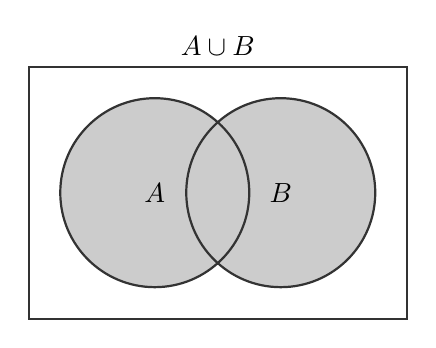
\begin{tikzpicture}[scale=0.8]
    \draw[outline] \vennRect;
    \draw[filled] \vennCircA \vennCircB;
    \node[anchor=south] at (current bounding box.north) {$A \cup B$};
\end{tikzpicture}
\caption{Venn diagram for set union}
\label{fig:union}
\end{figure}

\begin{definition}
$A\cap B\triangleq\set{x\mid x\in A\wedge x\in B}$
\end{definition}
เขียนเป็น Venn diagram ได้ดังรูปที่~\ref{fig:intersection}
%
\begin{figure}
\centering
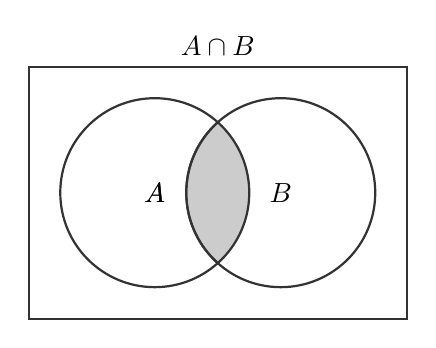
\begin{tikzpicture}[scale=0.8]
    \draw[outline] \vennRect;
    \begin{scope}
        \clip \vennCircA;
        \fill[filled] \vennCircB;
    \end{scope}
    \draw[outline] \vennCircA \vennCircB;
    \node[anchor=south] at (current bounding box.north) {$A \cap B$};
\end{tikzpicture}
\caption{Venn diagram for set intersection}
\label{fig:intersection}
\end{figure}

\begin{definition}
$A-B\triangleq\set{x\mid x\in A\wedge x\notin B}$
\end{definition}
เขียนเป็น Venn diagram ได้ดังรูปที่~\ref{fig:difference}
%
\begin{figure}
\centering
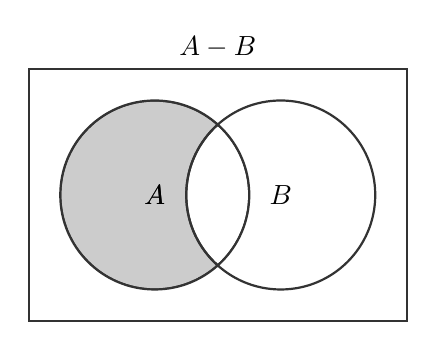
\begin{tikzpicture}[scale=0.8]
    \draw[outline] \vennRect;
    \begin{scope}
        \clip \vennCircA;
        \draw[filled, even odd rule] \vennCircA \vennCircB;
    \end{scope}
    \draw[outline] \vennCircA \vennCircB;
    \node[anchor=south] at (current bounding box.north) {$A-B$};
\end{tikzpicture}
\caption{Venn diagram for set difference}
\label{fig:difference}
\end{figure}

\begin{definition}
ให้ $D$ เป็นโดเมนที่เราสนใจ \enskip $\overline{A}\triangleq D-A$
\end{definition}
เขียนเป็น Venn diagram ได้ดังรูปที่~\ref{fig:complement}
%
\begin{figure}
\centering
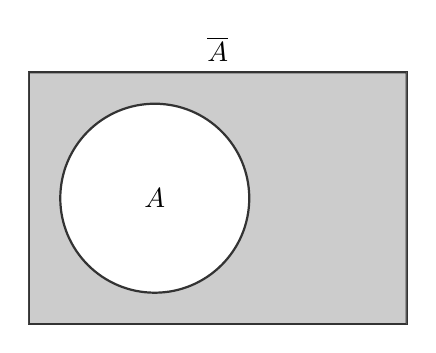
\begin{tikzpicture}[scale=0.8]
    \draw[outline] \vennRect;
    \begin{scope}
        \clip \vennRect;
        \draw[filled, even odd rule] \vennRect \vennCircA;
    \end{scope}
    \node[anchor=south] at (current bounding box.north) {$\overline{A}$};
\end{tikzpicture}
\caption{Venn diagram for set complement}
\label{fig:complement}
\end{figure}

ถัดไป จะกล่าวถึงความสัมพันธ์ระหว่างเซต

\begin{definition}
$A$ เป็น\emph{เซตย่อย} (subset) ของ $B$ [denoted $A\subseteq B$] หาก $\forall x: x\in A\implies x\in B$
\end{definition}
หากเขียนความสัมพันธ์ของเซต $A$ และ $B$ ในนิยามดังกล่าวเป็น\emph{แผนภาพเวนน์} (Venn diagram) จะได้ดังรูปที่~\ref{fig:subset}
\begin{figure}
\centering
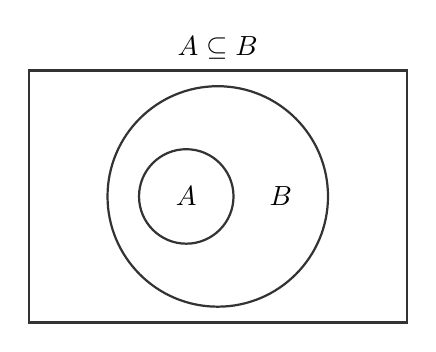
\begin{tikzpicture}[scale=0.8]
\draw[outline] \vennRect;
\draw[outline] {{(0.5,0) circle (0.75cm)} node {$A$}};
\draw[outline] {{(0:1cm) circle (1.75cm)}};
\node at (2,0) {$B$};
\node[anchor=south] at (current bounding box.north) {$A \subseteq B$};
\end{tikzpicture}
\caption{Venn diagram for subset}
\label{fig:subset}
\end{figure}
%
\begin{example}
$\mathbb{N}\subseteq\mathbb{Q}$
\end{example}
\begin{example}
ให้ $A=\set{1,2,\set{3,4}}$ จะได้ว่า
\begin{itemize}
\item $\set{1,2}\subseteq A$
\item $\set{3,4}\in A$
\item $\set{\set{3,4}}\subseteq A$
\item $\emptyset\subseteq A$ \enskip ทั้งนี้ เนื่องจาก $\forall x: x\in\emptyset\implies x\in A$ เนื่องจาก $x\in\emptyset$ นั้นเป็นจริงโดยปริยาย
\end{itemize}
\end{example}

\begin{theorem}
ให้ $A=\set{x\in\mathbb{Z}: 6\mid x}$ และ $B=\set{x\in\mathbb{Z}: 2\mid x}$ จะได้ว่า $A\subseteq B$
\begin{pf}
ต้องพิสูจน์ว่า $\forall x: x\in A\implies x\in B$ \enskip สมมุติว่า $x\in A$ กล่าวคือ $6\mid x$ แสดงว่ามี $x\in\mathbb{Z}$ ที่ทำให้ $x=6y$ นั่นคือ $x=2(3y)$ แต่นั่นแปลว่า $2\mid x$ จึงสรุปได้ว่า $x\in B$

ดังนั้น $A\subseteq B$ ตามที่ต้องการ
\end{pf}
\end{theorem}

\begin{theorem}
ให้ $A=\set{x\in\mathbb{Z}\mid x=y+z\ \textup{โดยที่ $y,z$ เป็นเลขคู่}}$ และ $B=\set{x\in\mathbb{Z}\mid x\ \textup{เป็นเลขคู่}}$ จะได้ว่า $A\subseteq B$
\begin{pf}
ให้ $x\in A$ นั่นคือ $x=y+z$ (ตามนิยามของ $A$) โดยที่ $y,z$ เป็นเลขคู่ \enskip จาก Theorem~2 ใน Lecture~3 จะได้ว่า $x$ เป็นเลขคู่ด้วย นั่นคือ $x\in B$ (ตามนิยามของ $B$) \enskip ดังนั้น เนื่องจากเราได้พิสูจน์ว่า $x\in B$ จากสมมุติฐานว่า $x\in A$ จะได้ว่า $A\subseteq B$ ตามที่ต้องการ
\end{pf}
\end{theorem}

\begin{theorem}
ให้ $a,b\in\mathbb{Z}$ \enskip ให้ $A=\set{x\in\mathbb{Z}:a\mid x}$ และ $B=\set{x\in\mathbb{Z}:b\mid x}$ จะได้ว่า \[A\subseteq B\iff b\mid a\]
\begin{pf}
($\Rightarrow$) เนื่องจาก $A\subseteq B$ จะได้ว่า $\forall x\in A: x\in B$ \enskip นอกจากนี้ $a\in A$ เพราะ $a\mid a$ \enskip ดังนั้น $a\in B$ เพราะ $A\subseteq B$ \enskip นั่นคือ $b\mid a$ ตามนิยามของเซต $B$

ในที่นี้ $b\mid a$ เป็น\emph{เงื่อนไขที่จำเป็น} (necessary condition) ของ $A\subseteq B$ กล่าวคือ หาก $A\subseteq B$ แล้ว $b\mid a$ อย่างแน่นอน

($\Leftarrow$) เนื่องจาก $b\mid a$ จะได้ว่า $a=bn$ โดยที่ $n\in\mathbb{Z}$ \enskip ให้ $x\in A$ กล่าวคือ $a\mid x$ จะได้ว่า $x=ak$ โดยที่ $k\in\mathbb{Z}$ \enskip ดังนั้น $x=bnk$ นั่นคือ $b\mid x$ ซึ่งแปลว่า $x\in B$ ตามนิยามของ $B$ \enskip เพราะฉะนั้น $A\subseteq B$

ในที่นี้ $b\mid a$ เป็น\emph{เงื่อนไขที่เพียงพอ} (sufficient condition) ของ $A\subseteq B$ กล่าวคือ แค่เพียง $b\mid a$ ก็พอที่ทำให้ $A\subseteq B$
\end{pf}
\end{theorem}

\begin{definition}[set equality]
$A=B$ หาก $\forall x: x\in A\iff x\in B$
\end{definition}
%
\begin{theorem}
$A=B$ iff $A\subseteq B$ และ $B\subseteq A$
\begin{pf}
($\Rightarrow$) ให้ $A=B$ กล่าวคือ $\forall x: x\in A\implies x\in B$ ต้องพิสูจน์ว่า $A\subseteq B$ และ $B\subseteq A$

พิจารณา $x$ ใดๆ \enskip เนื่องจาก $x\in A\iff x\in B$ (จาก $A=B$) จะได้ว่า
\begin{itemize}
\item $x\in A\implies x\in B$ นั่นคือ $A\subseteq B$
\item $x\in B\implies x\in A$ นั่นคือ $B\subseteq A$
\end{itemize}
ดังนั้น $A\subseteq B$ และ $B\subseteq A$ ตามที่ต้องการ

($\Leftarrow$) สมมุติว่า $A\subseteq B$ และ $B\subseteq A$ ต้องพิสูจน์ว่า $A=B$

พิจารณา $x$ ใดๆ ต้องพิสูจน์ว่า $x\in A\iff x\in B$\enskip เนื่องจาก
\begin{itemize}
\item $x\in A\implies x\in B$ (จาก $A\subseteq B$)
\item $x\in B\implies x\in A$ (จาก $B\subseteq A$)
\end{itemize}
จะได้ว่า $x\in A\iff x\in B$ กล่าวคือ $A=B$ นั่นเอง ตามที่ต้องการ
\end{pf}
\end{theorem}

\subsection{Connections between logic and sets}

ตัวดำเนินการเกี่ยวกับเซต และความสัมพันธ์ระหว่างเซต สามารถเชื่อมโยงกับตัวดำเนินการทางตรรกะได้ดังนี้
\begin{itemize}[]
\item ตัวดำเนินการ and ($\wedge$) นั้นเทียบเคียงได้กับตัวดำเนินการ intersection ($\cap$) เนื่องจากประพจน์ทั้งสองต้องเป็นจริง ประพจน์ผลลัพธ์จึงจะเป็นจริง และสมาชิกต้องอยู่ในทั้งสองเซต สมาชิกดังกล่าวจึงจะอยู่ใน intersection
\item ตัวดำเนินการ or ($\vee$) นั้นเทียบเคียงได้กับตัวดำเนินการ union ($\cup$) เนื่องจากประพจน์เพียงตัวใดตัวหนึ่งต้องเป็นจริง ประพจน์ผลลัพธ์จึงจะเป็นจริง และสมาชิกต้องอยู่ในเซตใดเซตหนึ่ง สมาชิกดังกล่าวจึงจะอยู่ใน union
\item ตัวดำเนินการ not ($\neg$) นั้นเทียบเคียงได้กับตัวดำเนินการ complement ($\overline{\cdot}$) เนื่องจากประพจน์ตั้งต้นต้องเป็นจริง ประพจน์ผลลัพธ์จึงจะเป็นเท็จ และสมาชิกต้องอยู่ในเซตตั้งต้น สมาชิกดังกล่าวจึงจะไม่อยู่ใน complement
\end{itemize}
จะเห็นว่า ตัวดำเนินการทั้งสามคู่ที่กล่าวมาข้างต้นนั้น รับข้อมูลนำเข้าเป็นประพจน์ หรือเซต และให้ผลลัพธ์เป็นประพจน์ หรือเซต เช่นเดียวกับข้อมูลนำเข้า
\begin{itemize}[]
\item ตัวดำเนินการ implication ($\implies$) นั้นเทียบเคียงได้กับความสัมพันธ์ subset ($\subseteq$) เนื่องจากประพจน์ผลลัพธ์จะเป็นจริงหากประพจน์ซ้ายเป็นจริงและประพจน์ขวาเป็นจริง หรือหากประพจน์ขวาเป็นเท็จ เช่นเดียวกับการที่คุณสมบัติ subset จะเป็นจริงหากสมาชิกอยู่ในเซตหน้าและเซตหลัง หรือสมาชิกไม่อยู่ในเซตหน้า
\item ตัวดำเนินการ iff ($\iff$) นั้นเทียบเคียงได้กับความสัมพันธ์ equality ($=$) เนื่องจากประพจน์สองตัวจะสมมูลกัน หากมีค่าความจริงเหมือนกัน เช่นเดียวกับเซตสองเซตที่เท่ากัน หากมีสมาชิกเหมือนกัน
\end{itemize}
จะเห็นว่า ความสัมพันธ์ทั้งสองคู่หลังนี้ รับข้อมูลนำเข้าเป็นประพจน์ หรือเซต แต่ให้ผลลัพธ์เป็นประพจน์เสมอ (นั่นคือ ผลลัพธ์เป็นจริงหรือเท็จ)

ความเชื่อมโยงดังที่ได้กล่าวมา สามารถสรุปได้ดังตารางต่อไปนี้
\begin{center}
\begin{tabular}{cc||cc}
\multicolumn{2}{c||}{\bf logic} & \multicolumn{2}{c}{\bf sets} \\ \hline
ชนิดตัวดำเนินการ & logical operator & set operator & ชนิดตัวดำเนินการ \\ \hline\hline
\ldelim\{{2}{4cm}[$\mathrm{Prop}\times\mathrm{Prop}\to\mathrm{Prop}$ ] & $\wedge$ & $\cap$ & \rdelim\}{2}{3.5cm}[ $\mathrm{Set}\times\mathrm{Set}\to\mathrm{Set}$] \\
& $\vee$ & $\cup$ & \\
$\mathrm{Prop}\to\mathrm{Prop}$ & $\neg$ & $\overline{\cdot}$ & $\mathrm{Set}\to\mathrm{Set}$ \\ \hline
\ldelim\{{2}{4cm}[$\mathrm{Prop}\times\mathrm{Prop}\to\mathrm{Prop}$ ] & $\implies$ & $\subseteq$ & \rdelim\}{2}{3.5cm}[ $\mathrm{Set}\times\mathrm{Set}\to\mathrm{Prop}$] \\
& $\iff$ & $=$ &
\end{tabular}
\end{center}

\subsection{Power sets}

\begin{definition}
ให้ $A$ เป็นเซต \enskip \emph{เซตกำลัง} (power set) ของ $A$ (denoted $\pow(A)$) คือเซต $\set{X\mid X\subseteq A}$
\end{definition}
บางครั้ง เราอาจจะเห็น power set ของ $A$ ที่เขียนด้วย $\mathcal{P}(A)$ หรือ $2^A$
%
\begin{example}
$\pow(\set{1,2})=\set{\emptyset,\set{1},\set{2},\set{1,2}}$
\end{example}
%
\begin{theorem}
$x\in A\iff\set{x}\in\pow(A)$
\begin{pf}
จากนิยามของ $\subseteq$ และ power set จะได้ว่า
$x\in A\iff\set{x}\subseteq A\iff\set{x}\in\pow(A)$
\end{pf}
\end{theorem}
ทั้งนี้ ในบทพิสูจน์ข้างต้น $x\in A\iff\set{x}\subseteq A$ อาจจะยังไม่ชัดเจนมากนัก จึงอาจเขียนเป็น\emph{บทตั้ง} (lemma) พร้อมบทพิสูจน์ที่ชัดเจนขึ้นได้ดังนี้
\begin{lemma}
$x\in A\iff\set{x}\subseteq A$
\begin{pf}
($\Rightarrow$): สมมุติว่า $x\in A$ ต้องพิสูจน์ว่า $\set{x}\subseteq A$ กล่าวคือ $\forall y: y\in\set{x}\implies y\in A$ \enskip ให้ $y\in\set{x}$ แสดงว่ามีค่าของ $y$ ที่เป็นไปได้เพียงตัวเดียวเท่านั้น กล่าวคือ $y=x$ \enskip ดังนั้น $y\in A$ เนื่องจาก $x\in A$ \qquad\yea

($\Leftarrow$): สมมุติว่า $\set{x}\subseteq{A}$ ต้องพิสูจน์ว่า $x\in A$ \enskip เนื่องจาก $\set{x}\subseteq A$ แสดงว่า $\forall y: y\in\set{x}\implies y\in A$ \enskip หากเราเลือกให้ $y$ มีค่าเป็น $x$ จะเห็นว่า $y\in\set{x}$ \enskip ดังนั้น $x\in A$ ตามต้องการ \qquad\yea
\end{pf}
\end{lemma}

\begin{theorem}
ให้ $A$ และ $B$ เป็นเซต \enskip $\pow(A)\cup\pow(B)\subseteq\pow(A\cup B)$
\begin{pf}
จากนิยามของ $\subseteq$ หากให้ $x\in\pow(A)\cup\pow(B)$ เราต้องพิสูจน์ว่า $x\in\pow(A\cup B)$ \enskip เนื่องจาก $x\in\pow(A)\cup\pow(B)$ แสดงว่า $x\in\pow(A)$ หรือ $x\in\pow(B)$ ตามนิยามของ $\cup$ \enskip พิสูจน์โดยแยกกรณีดังนี้
\begin{enumerate}[]
\item\label{pf:powset-union-subset-l} $x\in\pow(A)$: จะได้ว่า $x\subseteq A$ (ตามนิยามของ power set) \enskip ดังนั้น $x\subseteq A\cup B$
\item $x\in\pow(B)$: ในกรณีนี้ เราสามารถใช้เหตุผลเช่นเดียวกับในกรณีที่~\ref{pf:powset-union-subset-l} โดยสลับบทบาทของ $A$ และ $B$ \enskip จึงสรุปได้ว่า $x\in\pow(A\cup B)$ เช่นกัน
\end{enumerate}
ในทั้งสองกรณี เราสามารถสรุปได้ว่า $x\in\pow(A\cup B)$ \enskip ดังนั้น $\pow(A)\cup\pow(B)\subseteq\pow(A\cup B)$ ตามที่เราต้องการ
\end{pf}
\end{theorem}

\section{Lists}
\emph{รายการ} (lists) เป็น collections อีกชนิดหนึ่งที่มีสมบัติดังนี้
\begin{itemize}[]
\item สมาชิกซ้ำได้ (repetitions allowed)
\item ลำดับสำคัญ (ordered)
\end{itemize}
ในส่วนนี้ เราจะพิจารณาเฉพาะ lists ที่กำหนดความยาวแน่นอนก่อน \enskip Lists ในลักษณะนี้เรียกว่า \emph{tuples} ซึ่งสามารถสร้างขึ้นได้โดยใช้ Cartesian product
\begin{definition}
ให้ $A$ และ $B$ เป็นเซต \enskip \emph{ผลคูณคาร์ทีเซียน} (Cartesian product) ของ $A$ และ $B$ [denoted $A\times B$] คือเซตของ\emph{คู่อันดับ} (ordered pairs) ทั้งหมด โดยที่ตัวหน้าของคู่อันดับเป็นสมาชิกของ $A$ และตัวหลังของคู่อันดับเป็นสมาชิกของ $B$ กล่าวคือ
\[A\times B\triangleq\set{(a,b)\mid a\in A\wedge b\in B}\]
\end{definition}
%
\begin{example}\label{ex:Cartesian}
ให้ $A=\set{\str{d},\str{p}}$ และ $B=\set{\str{c},\str{x}}$ จะได้ว่า $A\times B=\set{(\str{d},\str{c}),(\str{d},\str{x}),(\str{p},\str{c}),(\str{p},\str{x})}$ และ $B\times A=\set{(\str{c},\str{d}),(\str{c},\str{p}),(\str{x},\str{d}),(\str{x},\str{p})}$
\end{example}
จะเห็นว่า $A\times B\neq B\times A$ กล่าวคือ Cartesian product ไม่มีสมบัติการสลับที่

เมื่อเราสร้าง ordered pairs ได้แล้ว เราสามารถสร้าง tuples ได้โดยใช้ Cartesian products ซ้ำกันหลายๆ ครั้ง ดังนี้ \enskip ให้ $A$, $B$, และ $C$ เป็นเซต และเราต้องการสร้าง tuples ที่มีความยาว 3 โดยตำแหน่งแรกเป็นสมาชิกของ $A$ ตำแหน่งที่สองเป็นสมาชิกของ $B$ และตำแหน่งสุดท้ายเป็นสมาชิกของ $C$ \enskip เริ่มแรก ให้หา Cartesian product $A\times B$ ก่อน จากนั้นนำผลลัพธ์ที่ได้ไปทำ Cartesian product กับ $C$ อีกครั้งหนึ่ง ได้ผลลัพธ์ดังนี้
\[(A\times B)\times C =\set{(x,c)\mid x\in A\times B\wedge c\in C}\]
แต่เนื่องจาก $x\in A\times B$ จะเห็นว่า $x$ นั้นต้องอยู่ในรูปคู่อันดับ $(a,b)$ โดยที่ $a\in A$ และ $b\in B$ กล่าวคือ
\[(A\times B)\times C =\set{((a,b),c)\mid (a\in A\wedge b\in B)\wedge c\in C}\]
อย่างไรก็ดี เราสามารถลบวงเล็บชั้นในที่ล้อมรอบ $a$ และ $b$ ออกได้โดยไม่เสียตำแหน่งของ $a$ และ $b$ ในผลลัพธ์ \enskip นอกจากนี้ Cartesian product นั้นมีสมบัติการเปลี่ยนหมู่ กล่าวคือ
\[(A\times B)\times C = A\times B\times C = A\times (B\times C)\]
ดังนั้น เราจึงเขียนเซตผลลัพธ์ใหม่ได้เป็น
\[A\times B\times C = \set{(a,b,c)\mid a\in A\wedge b\in B\wedge c\in C}\]
ซึ่งทำให้เราได้ tuples ที่มีความยาวเป็น 3 \enskip หากต้องการ tuples ที่มีความยาวมากกว่านี้ สามารถใช้วิธีเดียวกัน โดยเพิ่มจำนวนเซตที่นำมา Cartesian product กัน

ทั้งนี้ หากเราต้องการสร้าง $n$-tuples (tuples ที่มีความยาว $n$) โดยที่สมาชิกในแต่ละตำแหน่งนั้นมาจากเซต $A$ ทั้งหมด เราสามารถเขียนสัญกรณ์ (notation) ได้เป็น $A^n\triangleq\underbrace{A\times A\times\cdots\times A}_{\textrm{$n$ ตัว}}$

\section{Relations}

\emph{ความสัมพันธ์} (relation) เชื่อมโยงสิ่งสองสิ่งเข้าด้วยกัน
%
\begin{example}
$a$ กับ $b$ สัมพันธ์กันถ้า $a$ แต่งงานกับ $b$
\end{example}
\begin{example}
$a$ กับ $b$ สัมพันธ์กันถ้า $a$ ชอบ $b$
\end{example}
%
จะเห็นว่า ลำดับก่อนหลังในความสัมพันธ์มีความสำคัญ

\begin{definition}
ให้ $A,B$ เป็นเซต \enskip \emph{ความสัมพันธ์จาก $A$ ไป $B$} (relation from $A$ to $B$) คือเซต $R\subseteq A\times B$

เรียก $A$ ว่า\emph{โดเมน} (domain) และ $B$ ว่า\emph{โดเมนร่วมเกี่ยว} (codomain)\footnote{ไม่ใช้คำว่า range เนื่องจากอาจจะทำให้สับสนกับ image ได้} ของ $R$
\end{definition}
%
\begin{example}\label{ex:rel-a-b}
ให้ $A=\set{\str{d},\str{p}}$ และ $B=\set{\str{c},\str{x}}$ (จาก Example~\ref{ex:Cartesian}) \enskip $R=\set{(\str{d},\str{c}),(\str{p},\str{x})}\subseteq A\times B$ 
\end{example}
เมื่อมีความสัมพันธ์ $R$ from $A$ to $B$ ที่สามารถเขียนแจกแจงสมาชิกในรูปของคู่อันดับได้ เราสามารถวาด\emph{กราฟ} (graph) ของ $R$ ได้ โดยแจกแจงสมาชิกของ domain (เซต $A$) ไว้ด้านซ้าย และสมาชิกของ codomain (เซต $B$) ไว้ด้านขวา แล้วโยงลูกศรเชื่อมจาก $a$ ไป $b$ หาก $(a,b)\in R$ ดังตัวอย่างต่อไปนี้ ซึ่งแสดงกราฟความสัมพันธ์ของ $R$ ใน Example~\ref{ex:rel-a-b}
\begin{center}
\begin{tikzpicture}
\node (d) {\str{d}};
\node (p) [below=of d] {\str{p}};
\node (c) [right=of d] {\str{c}};
\node (x) [right=of p] {\str{x}};

\draw[arrow] (d) -- (c);
\draw[arrow] (p) -- (x);
\end{tikzpicture}
\end{center}
ในขณะเดียวกัน หากมีกราฟของความสัมพันธ์ใดๆ เราก็สามารถเขียนแจกแจงเป็นเซตได้เช่นกัน
%
\begin{example}
ให้ $A=\set{1,2,3,4}$ และ $B=\set{a,b,c,d}$ \enskip หากมีกราฟความสัมพันธ์ $R$ ดังนี้
\begin{center}
\begin{tikzpicture}
\node (A1) {$1$};
\node (A2) [below of=A1] {$2$};
\node (A3) [below of=A2] {$3$};
\node (A4) [below of=A3] {$4$};

\node (Ba) [right=1in of A1] {$a$};
\node (Bb) [below of=Ba] {$b$};
\node (Bc) [below of=Bb] {$c$};
\node (Bd) [below of=Bc] {$d$};

\path (A1) -- node[above=2ex] {$R$} (Ba);

\draw[->] (A1) -- (Ba);
\draw[->] (A1) -- (Bb);
\draw[->] (A3) -- (Bc);
\draw[->] (A4) -- (Bb);
\end{tikzpicture}
\end{center}
จะได้ว่า $R=\set{(1,a),(1,b),(3,c),(4,b)}$ \enskip นอกจากนี้ เราสามารถนับจำนวนลูกศรขาออกจากสมาชิกแต่ละตัวทางด้านซ้าย และจำนวนลูกศรขาเข้าไปยังสมาชิกแต่ละตัวทางด้านขวาได้ ตัวอย่างเช่น $1$ มี 2 ลูกศรออก, $2$ มี 0 ลูกศรออก, $b$ มี 2 ลูกศรเข้า, และ $c$ มี 1 ลูกศรเข้า
\end{example}

\begin{example}
ให้ $A$ เป็นเซตของนักศึกษา และ $B$ เป็นเซตของวิชา \enskip $R=\set{(a,b)\mid\text{$a$ ลงทะเบียนวิชา $b$}}$
\end{example}

\begin{example}
ให้ $A$ เป็นเซตผู้ชาย และ $B$ เป็นเซตของผู้หญิง \enskip $R=\set{(a,b)\mid\text{$a$ ชอบ $b$}}$
\end{example}

\begin{definition}
ให้ $A$ เป็นเซต \enskip \emph{ความสัมพันธ์บนเซต $A$} (relation on $A$) คือเซต $R\subseteq A\times A$
\end{definition}
%
\begin{example}
ให้ $A=\set{\str{d},\str{p}}$ (จาก Example~\ref{ex:Cartesian}) \enskip \[R=\set{(\str{d},\str{p}),(\str{p},\str{d})}\subseteq A\times A=\set{(\str{d},\str{d}),(\str{d},\str{p}),(\str{p},\str{d}),(\str{p},\str{p})}\]
\end{example}
%
\begin{example}
$\leq$ is a relation on $\mathbb{Z}$.

\[\leq\ =\set{(0,0),(0,1),(-1,0),(-2,-1),(2019,2562),\ldots}\]
\end{example}

\begin{example}
$=$, $<$, $>$, $\geq$, $\neq$ are relations on $\mathbb{Z}$, $\mathbb{Q}$, $\mathbb{R}$
\end{example}

\begin{example}
ให้ $A$ เป็นเซตของ \textit{homo sapiens sapiens} \enskip $R=\set{(a_1,a_2)\mid\text{$a_1$ ชอบ $a_2$}}$ is a relation on $A$
\end{example}

\begin{definition}
ให้ $R$ เป็น relation \enskip \emph{ความสัมพันธ์ผกผัน} (inverse) ของ $R$ (denoted $R^{-1}$) คือเซต \[R^{-1}\triangleq\set{(b,a)\mid(a,b)\in R}\]
\end{definition}
%
\begin{example}
ให้ $R=\set{(\str{d},\str{c}),(\str{p},\str{x})}$ จะได้ว่า $R^{-1}=\set{(\str{c},\str{d}),(\str{x},\str{p})}$
\end{example}

\begin{example}
ให้ $R=\set{(a_1,a_2)\mid\text{$a_1$ ชอบ $a_2$}}$ จะได้ว่า $R^{-1}=\set{(a_1,a_2)\mid\text{$a_2$ ชอบ $a_1$}}$
\end{example}

\begin{definition}
ให้ $R\subset A\times B$ และ $a\in A$ \enskip \emph{ภาพ} (image) ของ $a$ ภายใต้ $R$ (denoted $R(a)$) คือเซต \[R(a)\triangleq\set{b\in B\mid (a,b)\in R}\]
\end{definition}
\begin{definition}
ให้ $R\subset A\times B$ และ $A'\subseteq A$ \enskip \emph{image of $A'$ under $R$} (denoted $R(A')$) คือเซต
\begin{align*}
R(A')&\triangleq\set{b\in B\mid\exists a\in A': (a,b)\in R} \\
&=\bigcup_{a\in A'}{R(a)}
\end{align*}
\end{definition}
%
\begin{example}
ให้ $R=\set{(1,4),(1,5),(2,6),(3,6)}$ จะได้ว่า
\begin{itemize}
\item $R(1)=\set{4,5}$
\item $R(2)=\set{6}$
\item $R^{-1}(4)=\set{1}$
\item $R^{-1}(6)=\set{2,3}$
\item $R(\set{1,2})=\set{4,5,6}$
\item $R(\set{2,3})=\set{6}$
\item $R^{-1}(\set{4,5})=\set{1}$
\item $R^{-1}(\set{6})=\set{2,3}$
\item $R(A)=\set{4,5,6}$
\end{itemize}
\end{example}
จะเห็นว่า image ของสมาชิกหรือเซตย่อยของโดเมนนั้น ก็คือ subset ของ codomain ที่มีลูกศรชี้ไปหาจากสมาชิกหรือเซตย่อยที่เรากำลังพิจารณาอยู่ \enskip หากเซตย่อยที่เรากำลังพิจารณานั้นเป็นทั้งโดเมน จะได้ผลลัพธ์เป็นสมาชิกใน codomain ที่ปรากฎอยู่ในความสัมพันธ์ ซึ่งอาจจะไม่ครบทุกตัวก็ได้ \enskip ด้วยเหตุนี้ เราจึงหลีกเลี่ยงการใช้คำว่า range ในการอธิบายความสัมพันธ์ เนื่องจากเราอาจจะตีความว่า range เป็นสมาชิกที่เราสามารถสร้างลูกศรชี้ไปหาได้ (ซึ่งมีความหมายเดียวกับ codomain) หรืออาจจะตีความว่า range เป็นสมาชิกที่มีลูกศรในความสัมพันธ์ชี้ไปหาก็ได้ (ซึ่งมีความหมายเดียวกับ image)

\subsection{Properties of relations}

ใน Definitions~\ref{def:reflexive}--\ref{def:transitive} ให้ $R$ เป็น relation on $A$ \enskip เราสามารถนิยามคุณสมบัติของความสัมพันธ์แบบต่างๆ ได้ดังนี้

\begin{definition}\label{def:reflexive}
$R$ มีสมบัติ\emph{สะท้อน} (reflexive) หาก \[\forall x\in A: \R{x}{x}\]
\end{definition}
($\R{x}{x}$ เป็นอีกวิธีหนึ่งในการเขียน $(x,x)\in R$)

\begin{definition}
$R$ มีสมบัติ\emph{ไม่สะท้อน} (irreflexive) หาก \[\forall x\in A: \R[/\!\!\!R]{x}{x}\]
\end{definition}

\begin{definition}
$R$ มีสมบัติ\emph{สมมาตร} (symmetric) หาก \[\forall x,y\in A: \R{x}{y}\implies\R{y}{x}\]
\end{definition}

\begin{definition}
$R$ มีสมบัติ\emph{ปฏิสมมาตร} (antisymmetric) หาก \[\forall x,y\in A: \R{x}{y}\wedge\R{y}{x}\implies x=y\]
\end{definition}

\begin{definition}\label{def:transitive}
$R$ มีสมบัติ\emph{ถ่ายทอด} (transitive) หาก \[\forall x,y,z\in A: \R{x}{y}\wedge\R{y}{z}\implies\R{x}{z}\]
\end{definition}

\begin{example}
ความสัมพันธ์ต่างๆ ต่อไปนี้มีสมบัติดังปรากฏในตาราง
\begin{center}
\begin{longtable}{c|c||c|c|c|c|c}
$A$ & relation & \rotatedhdr{reflexive} & \rotatedhdr{irreflexive} & \rotatedhdr{symmetric} & \rotatedhdr{antisymmetric} & \rotatedhdr{transitive} \\ \hline\hline
\endhead
\multirow{3}{*}{$\mathbb{Z}$}
 & $=$ & \yea & \nay & \yea & \yea & \yea \\ \cline{2-7}
 & $\leq$ & \yea & \nay & \nay & \yea & \yea \\ \cline{2-7}
 & $<$ & \nay & \yea & \nay & \yea\footnote{เป็นจริงโดยปริยาย (vacuously true) เนื่องจากไม่มีจำนวนเต็ม $x$ และ $y$ ที่ $x<y$ และ $y<x$ ทั้งคู่} & \yea \\ \hline
\multirow{2}{*}{\it homo sapiens sapiens}
 & แต่งงาน\footnote{หาก $a$ แต่งงานกับ $b$ หมายถึง $a$ จดทะเบียนสมรสกับ $b$} & \nay & \yea & \yea & \nay & \nay \\ \cline{2-7}
 & ชอบ & \yea & \nay & \nay & \nay & \nay
\end{longtable}
\end{center}
\end{example}

ใน Definitions~\ref{def:function}--\ref{def:bijection} ให้ $R$ เป็น relation from $A$ to $B$ 

\begin{definition}\label{def:function}
$R$ เป็น\emph{ฟังก์ชัน} (function) หากสมาชิกทุกตัวใน $A$ มี $\leq 1$ ออก กล่าวคือ \[\forall a\in A: |R(a)|\leq 1\]
\end{definition}

\begin{definition}
$R$ นั้น\emph{ทุกส่วน} (total) หากสมาชิกทุกตัวใน $A$ มี $\geq 1$ ออก กล่าวคือ \[\forall a\in A: |R(a)|\geq 1\]
\end{definition}

\begin{definition}
$R$ นั้น\emph{หนึ่งต่อหนึ่ง}\footnote{หากใช้ภาษาไทย อาจจะสับสนกับ bijection ได้} (injection) หากสมาชิกทุกตัวใน $B$ มี $\leq 1$ เข้า กล่าวคือ \[\forall b\in B: |R^{-1}(b)|\leq 1\]
\end{definition}

\begin{definition}
$R$ นั้น\emph{ทั่วถึง} (surjection) หากสมาชิกทุกตัวใน $B$ มี $\geq 1$ เข้า กล่าวคือ \[\forall b\in B: |R^{-1}(b)|\geq 1\]
\end{definition}

\begin{definition}\label{def:bijection}
$R$ นั้น\emph{หนึ่งต่อหนึ่งทั่วถึง}\footnote{หากใช้ภาษาไทย อาจจะลืมว่าเป็น total function ได้} (bijection) หากสมาชิกทุกตัวใน $A$ มี $=1$ ออก และสมาชิกทุกตัวใน $B$ มี $=1$ เข้า กล่าวคือ \[\forall a\in A: |R(a)|= 1 \wedge \forall b\in B: |R^{-1}(b)|= 1\]
\end{definition}

\begin{example}
ความสัมพันธ์ต่างๆ ต่อไปนี้มีสมบัติดังปรากฏในตาราง
\begin{center}
\begin{longtable}{c|c|c||c|c|c|c|c}
$A$ & $B$ & relation & \rotatedhdr{function} & \rotatedhdr{total} & \rotatedhdr{injection} & \rotatedhdr{surjection} & \rotatedhdr{bijection} \\ \hline\hline
\endhead
\multirow{4}{0.6in}{\centering $\mathbb{R}$} & \multirow{4}{0.6in}{\centering $\mathbb{R}$}
 & $\R{x}{2x}$ & \yea & \yea & \yea & \yea & \yea \\ \cline{3-8}
 & & $\R{x}{\frac{1}{x}}$ & \yea & \nay\footnote{หากเป็น function ที่ไม่ total จะเรียกว่า\emph{ฟังก์ชันบางส่วน} (partial function)} & \yea & \nay & \nay \\ \cline{3-8}
 & & $\R{x^2}{x}$ & \nay & \nay & \yea & \yea & \nay \\ \cline{3-8}
 & & $\leq$ & \nay & \yea & \nay & \yea & \nay \\ \hline
\multicolumn{2}{c|}{\multirow{2}{*}{\it homo sapiens sapiens}}
 & แต่งงาน\footnote{สมบัติต่างๆ อาจขึ้นกับความเชื่อส่วนบุคคล โปรดใช้วิจารณญาณในการอ่าน} & \yea & \nay & \yea & \nay & \nay \\ \cline{3-8}
\multicolumn{2}{c|}{}
 & ชอบ & \nay & \nay & \nay & \nay & \nay
\end{longtable}
\end{center}
\end{example}

\subsection{Relational compositions}
เราสามารถนำความสัมพันธ์มาเกี่ยวโยงกันได้
\begin{definition}
ให้ $R$ เป็น relation from $A$ to $B$ และ $S$ เป็น relation from $B$ to $C$ \enskip \emph{ความสัมพันธ์ประกอบ} (composition) ของ $R$ และ $S$ (denoted $S\circ R$) คือเซต \[S\circ R\triangleq\set{(a,c)\mid\exists b\in B: \R{a}{b} \wedge \R[S]{b}{c}}\]
\end{definition}
นั่นคือ เราสามารถสร้างความสัมพันธ์ที๋มีลูกศรโยงจากสมาชิกในเซต $A$ ไปยังสมาชิกในเซต $C$ ได้ หากมีสมาชิกในเซต $B$ ที่เป็นตัวกลางเชื่อมสมาชิกทั้งสองเซตก่อนหน้านี้ กล่าวคือ มีลูกศรโยงจากสมาชิกในเซต $A$ ไปยังสมาชิกในเซต $B$ และมีลูกศรโยงจากสมาชิกตัวนี้ในเซต $B$ ไปยังสมาชิกในเซต $C$
%
\begin{example}
นิยาม $R$ และ $S$ ตามกราฟต่อไปนี้
\begin{center}
\begin{tikzpicture}
\node (A1) {$\pi$};
\node (A2) [below of=A1] {$\sqrt{2}$};

\node (B1) [right=1in of A1] {$1$};
\node (B2) [below of=B1] {$2$};
\node (B3) [below of=B2] {$3$};
\node (B4) [below of=B3] {$4$};

\node (Ca) [right=1in of B1] {$a$};
\node (Cb) [below of=Ca] {$b$};
\node (Cc) [below of=Cb] {$c$};
\node (Cd) [below of=Cc] {$d$};

\path (A1) -- node[above=2ex] {$R$} (B1) -- node[above=2ex] {$S$} (Ca);

\draw[->] (A1) -- (B2);
\draw[->] (A1) -- (B4);
\draw[->] (A2) -- (B1);

\draw[->] (B1) -- (Ca);
\draw[->] (B1) -- (Cb);
\draw[->] (B3) -- (Cc);
\draw[->] (B4) -- (Cb);
\end{tikzpicture}
\end{center}
จะได้ว่า $S\circ R=\set{(\sqrt{2},a),(\sqrt{2},b),(\pi,b)}$
\end{example}
%
\begin{example}
ให้ $f(x)=x+1$ และ $g(x)=x^2$ จะได้ว่า
\begin{align*}
(g\circ f)(x)
&= g(f(x)) \\
&= g(x+1) \\
&= (x+1)^2
\end{align*}
หากเขียนในรูปความสัมพันธ์ จะได้ว่า $\R[f]{x}{(x+1)}$ และ $\R[g]{x}{x^2}$ กล่าวคือ $\R[g]{(x+1)}{(x+1)^2}$ \enskip ดังนั้น \[\R[(g\circ f)]{x}{(x+1)^2}\]
\end{example}

\begin{example}
ให้ $A$ เป็นเซตของนักศึกษามหาวิทยาลัยเชียงใหม่, $B$ เป็นเซตของกระบวนวิชาในมหาวิทยาลัยเชียงใหม่, และ $C$ เป็นเซตของอาจารย์มหาวิทยาลัยเชียงใหม่ \enskip ให้ $R\subseteq A\times B$ เป็นความสัมพันธ์ระหว่างนักศึกษา $a$ กับกระบวนวิชา $b$ โดยที่ $\R{a}{b}$ หาก $a$ ลงทะเบียนเรียนวิชา $b$ ในภาคเรียนนี้, และ $S\subseteq B\times C$ เป็นความสัมพันธ์ระหว่างกระบวนวิชา $b$ กับอาจารย์ $c$ โดยที่ $\R[S]{b}{c}$ หาก $c$ สอนวิชา $b$ ในภาคเรียนนี้ \enskip จะได้ว่า
\begin{itemize}[]
\item $R(A)$ (image of $A$ under $R$) เป็นเซตของวิชาที่มีนักศึกษาลงทะเบียนในภาคเรียนนี้ (นั่นคือ วิชาใดมีลูกศรชี้มาจากนักศึกษาบ้างในความสัมพันธ์ $R$)
\item $S^{-1}(\text{ชิน})$ (image of ชิน under $S^{-1}$) เป็นเซตของวิชาที่ อ.ชินสอนในภาคเรียนนี้ (นั่นคือ วิชาใดมีลูกศรชี้ไปหา อ.ชินบ้างในความสัมพันธ์ $S$)
\item $S\circ R\subseteq A\times C$ เป็นความสัมพันธ์ที่เชื่อมโยงนักศึกษากับอาจารย์ โดยที่ $\R[S\circ R]{a}{c}$ หากนักศึกษา $a$ เรียนกับอาจารย์ $c$
\item $R\circ R^{-1}\subseteq B\times B$ เป็นความสัมพันธ์ที่เชื่อมโยงสองวิชาเข้าด้วยกัน โดยที่ $\R[R\circ R^{-1}]{b_1}{b_2}$ หากวิชา $b_1$ และ $b_2$ ไม่สามารถจัดสอบปลายภาคพร้อมกันได้ เนื่องจากมีนักศึกษาที่ลงทะเบียนวิชา $b_1$ และ $b_2$ ทั้งคู่ (หรือ $b_1$ และ $b_2$ นี้เป็นวิชาเดียวกัน)
\item $R^{-1}\circ R\subseteq A\times A$ เป็นความสัมพันธ์ที่เชื่อมโยงนักศึกษาสองค้นเข้าด้วยกัน โดยที่ $\R[R^{-1}\circ R]{a_1}{a_2}$ หากนักศึกษา $a_1$ และ $a_2$ ลงทะเบียนเรียนวิชาเดียวกัน (หรือ $a_1$ และ $a_2$ เป็นนักศึกษาคนเดียวกัน)
\end{itemize}
\end{example}


\chapter{Induction}
\section{Inductive definitions}

บทนิยามแบบอุปนัย (inductive definitions) เป็นการกำหนดวิธีการสร้างวัตถุที่มีขนาดใหญ่ขึ้น จากวัตถุต่างๆ ที่มีขนาดเล็กกว่า

\begin{example}
นิพจน์เลขคณิต (arithmetic expressions) สามารถนิยามได้ดังนี้
\begin{itemize}
\item จำนวนตรรกยะ เป็น arithmetic expression
\item ตัวแปร ($x,y,z,\ldots$) เป็น arithmetic expression
\item[+] ถ้า $a_1$ และ $a_2$ เป็น arithmetic expressions แล้ว $a_1+a_2$, $a_1-a_2$, $a_1\times a_2$, และ $a_1\div a_2$ ก็เป็น arithmetic expressions ด้วย
\end{itemize}
ตัวอย่างของ arithmetic expressions จากนิยามดังกล่าวได้แก่ $1,0,-3,\frac{2}{3},x,z,x+z,x-(-3),24+48-56$ สังเกตว่า arithmetic expression แต่ละตัวสามารถแยกย่อยเป็น arithmetic expression(s) ที่เล็กกว่าได้เรื่อยๆ หาก arithmetic expression ตั้งต้นนั้นไม่ได้เล็กที่สุดอยู่แล้ว
\end{example}

\begin{example}\label{ex:ind-bexp}
นิพจน์บูลเลียน (boolean expressions) สามารถนิยามได้ดังนี้
\begin{itemize}
\item $\mathrm{true}$ เป็น boolean expression
\item $\mathrm{false}$ เป็น boolean expression
\item ถ้า $a_1$ และ $a_2$ เป็น arithmetic expressions แล้ว $a_1=a_2$, $a_1<a_2$, และ $a_1>a_2$ เป็น boolean expressions
\item[+] ถ้า $b$ เป็น boolean expression แล้ว $\neg b$ ก็เป็น boolean expression ด้วย
\item[+] ถ้า $b_1$ และ $b_2$ เป็น boolean expressions แล้ว $b_1\wedge b_2$ และ $b_1\vee b_2$ ก็เป็น boolean expressions ด้วย
\end{itemize}
\end{example}

\begin{definition}
\emph{บทนิยามแบบอุปนัย} (inductive definition) ประกอบด้วย 2 ส่วน
\begin{itemize}
\item \emph{กรณีฐาน} (base case) ซึ่งกำหนดวิธีการสร้างวัตถุตั้งต้น โดยไม่พึ่งพาวัตถุอื่นๆ ที่มีชนิดเดียวกันในการสร้างขึ้นมา
\item[+] \emph{กรณีอุปนัย} (inductive case) ซึ่งกำหนดวิธีการสร้างวัตถุที่มีขนาดใหญ่ขึ้น โดยมีวัตถุ\emph{ชนิดเดียวกัน}ที่มีขนาดเล็กกว่าเป็นส่วนประกอบอย่างน้อย 1 ชิ้น
\end{itemize}
\end{definition}
จากนิยามดังกล่าว จะเห็นว่าใน Example~\ref{ex:ind-bexp} การสร้าง boolean expressions จาก arithmetic expressions โดยใช้การเปรียบเทียบไม่ถือว่าเป็นกรณีอุปนัย เนื่องจากวัตถุที่เป็นส่วนประกอบไม่ใช่ boolean expressions เช่นเดียวกับผลลัพธ์

\begin{example}
รายการที่มีสมาชิกเป็นจำนวนเต็ม (integer lists) สามารถนิยามแบบอุปนัยได้ดังนี้
\begin{itemize}
\item{} [] (รายการว่าง / empty list) เป็น integer list (เรียกว่า $\mathrm{nil}$)
\item[+] ถ้า $\ell$ เป็น integer list และ $a\in\mathbb{Z}$ แล้ว $a:\ell$ ($a$ ตามด้วยสมาชิกตามลำดับใน $\ell$) ก็เป็น integer list ด้วย (เรียกว่า $\mathrm{cons}(a,\ell)$)
\end{itemize}
Integer lists ทั้งหมดที่เป็นไปได้สามารถสร้างได้ด้วยวิธีดังกล่าว ตัวอย่างเช่น หากต้องการสร้าง list ที่ประกอบไปด้วยสมาชิกสองตัว $[4,7]$ สามารถสร้างได้จากการนำ 7 มาปะหน้า empty list ได้ผลลัพธ์เป็น $7:[]$ แล้วนำ 4 มาปะหน้า list ดังกล่าว ได้ผลลัพธ์เป็น $4:(7:[])=\mathrm{cons}(4, \mathrm{cons}(7, \mathrm{nil}))$

หากจะแปลงนิยามแบบอุปนัยข้างต้นเป็นโปรแกรมในภาษา Java สามารถเขียนได้ดังนี้
\begin{lstlisting}[language=Java]
class Node {
  int hd;
  Node tl;
  ...
}
Node l1 = null;            // nil = []
Node l2 = new Node(7, l1); // cons(7, l1) = [7]
Node l3 = new Node(4, l2); // cons(4, l2) = [4, 7]
\end{lstlisting}
\end{example}

\begin{example}
โครงสร้างข้อมูลชนิดต้นไม้ที่มีสมาชิกเป็นจำนวนเต็ม (integer trees) สามารถนิยามแบบอุปนัยได้ดังนี้
\begin{itemize}[]
\item empty tree เป็น integer tree
\item[+] ถ้า $a\in\mathbb{Z}$ และ $t_1,t_2$ เป็น integer trees แล้ว $\mathrm{Tree}(a, t_1, t_2)$ (ต้นไม้ที่มี $a$ เป็นราก ต้นไม้ย่อยด้านซ้ายเป็น $t_1$ และต้นไม้ย่อยด้านขวาเป็น $t_2$) ก็เป็น integer tree ด้วย ดังรูป
\begin{center}
\begin{tikzpicture}
\node[circle,draw] (a) {$a$};
\node[draw,regular polygon, regular polygon sides=3,below left=of a] (t1) {$t_1$};
\node[draw,regular polygon, regular polygon sides=3,below right=of a] (t2) {$t_2$};
\draw (a) -- (t1.north);
\draw (a) -- (t2.north);
\end{tikzpicture}
\end{center}
\end{itemize}
หากจะแปลงนิยามแบบอุปนัยข้างต้นเป็นโปรแกรมในภาษา Java สามารถเขียนได้ดังนี้
\begin{lstlisting}[language=Java]
class Tree {
  int a;
  Tree left, right;
  ...
}
\end{lstlisting}
\end{example}

เมื่อมีนิยามแบบอุปนัย ก็สามารถนิยามตัวดำเนินการและฟังก์ชันต่างๆ เกี่ยวกับวัตถุชนิดนั้นๆ ได้โดยวิธีเวียนบังเกิด (recursion)
\begin{definition}
ให้ $\ell_1$ และ $\ell_2$ เป็น integer lists \enskip นิยาม\emph{การต่อกัน} (concatenation) ของ $\ell_1$ และ $\ell_2$ [denoted $\ell_1\lconcat\ell_2$] ดังนี้
\begin{itemize}
\item หาก $\ell_1=[]$ จะได้ $[]\lconcat\ell_2\triangleq\ell_2$ \\
กล่าวคือ หากจะนำ list ใดๆ มาต่อ empty list ก็จะได้ list นั้นๆ

\item หาก $\ell_1=a:\ell_1'$ จะได้ $(a:\ell_1')\lconcat\ell_2\triangleq a:(\ell_1'\lconcat\ell_2)$ \\
กล่าวคือ หากตัวหน้าไม่ใช่ empty list ก็ย่อมมีหัว ($a$) และหาง ($\ell_1'$) \enskip ผลลัพธ์ของ $\lconcat$ ก็คือ นำ $\ell_2$ ไปต่อท้าย $\ell_1'$ ก่อน โดยวิธีเวียนบังเกิด (recursion) ได้ผลลัพธ์เป็น $\ell_1'\lconcat\ell_2$ \enskip จากนั้น ค่อยนำ $a$ มาปะหน้าผลลัพธ์ดังกล่าว
\end{itemize}
\end{definition}
%
\begin{example}
ให้ $\ell_1=[2,5]$ และ $\ell_2=[4,7]$ เราสามารถหา $\ell_1\lconcat\ell_2$ ตามลำดับดังนี้
\begin{itemize}
\item $(2:5:[])\lconcat(4:7:[])=2:((5:[])\lconcat(4:7:[]))$
\item $(5:[])\lconcat(4:7:[])=5:([]\lconcat(4:7:[]))$
\item $[]\lconcat(4:7:[])=4:7:[]$
\item ดังนั้น $5:([]\lconcat(4:7:[]))=5:4:7:[]$
\item ดังนั้น $2:((5:[])\lconcat(4:7:[]))=2:(5:([]\lconcat(4:7:[])))=2:5:4:7:[]$
\end{itemize}
สรุปได้ว่า ผลลัพธ์คือ $[2,5,4,7]$
\end{example}


\section{Structural induction}

เมื่อมีตัวดำเนินการต่างๆ เกี่ยวกับวัตถุที่สร้างโดยใช้นิยามแบบอุปนัย ก็สามารถเขียนและพิสูจน์ทฤษฎีบทเกี่ยวกับตัวดำเนินการนั้นๆ ได้ ด้วยวิธี\emph{อุปนัยเชิงโครงสร้าง} (structural induction)

หลักการโดยคร่าวๆ ของวิธี structural induction เพื่อพิสูจน์ว่าคุณสมบัติ $P(x)$ เป็นจริงสำหรับวัตถุ $x$ ใดๆ มีสองขั้นตอน ได้แก่
\begin{itemize}[]
\item \emph{ขั้นฐาน} (base case): พิสูจน์ว่า $P(x)$ นั้นเป็นจริงกับวัตถุ $x$ ที่สร้างโดยกรณีฐาน
\item \emph{ขั้นอุปนัย} (inductive step): พิสูจน์ว่า $P(x)$ นั้นเป็นจริงกับวัตถุ $x$ ที่สร้างโดยกรณีอุปนัย โดยตั้งสมมุติฐานว่าคุณสมบัติ $P$ นั้นเป็นจริงกับวัตถุชิ้นย่อยๆ ที่เป็นส่วนประกอบของ $x$ \enskip กล่าวคือ หากวัตถุที่มีขนาดเล็กกว่ามีคุณสมบัติตามที่ต้องการ เมื่อนำมาประกอบเป็นวัตถุที่ใหญ่ขึ้น ก็จะยังมีคุณสมบัตินี้เช่นเดิม \enskip สมมุติฐาน $P$ ที่เราตั้งขึ้นนี้เรียกว่า\emph{สมมุติฐานในการอุปนัย} (induction hypothesis) โดยจากนี้ไป บทพิสูจน์ต่างๆ จะใช้ ``I.H.'' เพื่อย่อวลี induction hypothesis
\end{itemize}
หลังจากทำสองขั้นตอนนี้แล้ว เราสามารถสรุปได้ว่า ไม่ว่าเราจะประกอบวัตถุให้มีขนาดใหญ่เท่าใดก็ตาม วัตถุดังกล่าวก็ยังมีคุณสมบัติที่ต้องการเสมอ
%
ตัวอย่างเช่น
\begin{theorem}
ให้ $\ell$ เป็น integer list ใดๆ จะได้ว่า $\ell\lconcat[]=\ell$
\begin{pf}
By structural induction โดยที่ \[P(\ell)\triangleq \ell\lconcat[]=\ell\]
\begin{itemize}
\item {\bf Base case}: ($\ell=[]$) จะได้ว่า $[]\lconcat[]=[]$ ตามนิยามของ \lconcat{} \qquad\yea
\item {\bf Inductive step}: ($\ell=a:\ell'$) \quad สมมุติว่า $P(\ell')$ เป็นจริง กล่าวคือ $\ell'\lconcat[]=\ell'$ \enskip ต้องพิสูจน์ว่า $(a:\ell')\lconcat[]=a:\ell'$ \enskip จะเห็นว่า
\begin{align*}
(a:\ell')\lconcat[]
 &= a:(\ell'\lconcat []) \qquad\textup{(จากนิยามของ \lconcat)} \\
 &= a:\ell' \qquad\textup{(by I.H.)\qquad\yea}
\end{align*}
\end{itemize}
ดังนั้น จึงสรุปได้ว่า $\ell\lconcat[]=\ell$ ไม่ว่า $\ell$ จะมีสมาชิกกี่ตัวก็ตาม
\end{pf}
\end{theorem}

นั่นคือ การใช้ structural induction กับ integer lists เมื่อต้องการพิสูจน์ predicate $P(\ell)$ มีสองขั้นตอน
\begin{itemize}
\item base case: พิสูจน์ว่า $P([])$ เป็นจริง
\item inductive step: สมมุติว่า $P(\ell)$ เป็นจริงกับ $\ell$ ใดๆ ต้องพิสูจน์ว่า $P(a:\ell)$ เป็นจริงด้วย ไม่ว่า $a$ จะเป็นจำนวนเต็มใดๆ ก็ตาม
\end{itemize}
หลังจากสองขั้นตอนนี้แล้ว เราสามารถสรุปได้ว่า $P(\ell)$ เป็นจริงสำหรับ integer list $\ell$ ทุกตัว เนื่องจากเราได้แสดงให้เห็นแล้วว่า $P$ เป็นจริงในทุกวิธีที่เราสามารถสร้าง integer list ขึ้นมาได้

ลองดูอีกตัวอย่างหนึ่ง
\begin{theorem}
ให้ $\ell_1,\ell_2,\ell_3$ เป็น integer lists ใดๆ จะได้ว่า \[(\ell_1\lconcat\ell_2)\lconcat\ell_3=\ell_1\lconcat(\ell_2\lconcat\ell_3)\] กล่าวคือ $\lconcat$ มีสมบัติการเปลี่ยนหมู่ (associativity)
\begin{pf}
เราจะใช้ structural induction โดยแยกกรณีตามรูปร่างของ $\ell_1$ (นั่นคือ เราจะทำการพิสูจน์ by structural induction on $\ell_1$) \enskip ทั้งนี้ predicate ที่เราจะพิสูจน์โดยอุปนัยคือ \[P(\ell_1)\triangleq\forall\ell_2,\ell_3: (\ell_1\lconcat\ell_2)\lconcat\ell_3=\ell_1\lconcat(\ell_2\lconcat\ell_3)\]
\begin{itemize}
\item{\bf Base case}: ($\ell_1=[]$) \quad $([]\lconcat\ell_2)\lconcat\ell_3=\ell_2\lconcat\ell_3$ ตามนิยามของ \lconcat{} และ $[]\lconcat(\ell_2\lconcat\ell_3)=\ell_2\lconcat\ell_3$ ตามนิยามของ \lconcat{} ด้วย ทั้งสองข้างจึงเป็น $\ell_2\lconcat\ell_3$ เหมือนกัน \qquad\yea
\item{\bf Inductive step}: ($\ell_1=a:\ell_1'$) \quad สมมุติว่า $\forall\ell_2,\ell_3:(\ell_1'\lconcat\ell_2)\lconcat\ell_3=\ell_1'\lconcat(\ell_2\lconcat\ell_3)$ \enskip \enskip ต้องพิสูจน์ว่า $\forall\ell_2,\ell_3:((a:\ell_1')\lconcat\ell_2)\lconcat\ell_3=(a:\ell_1')\lconcat(\ell_2\lconcat\ell_3)$ โดยจะทำการแปลง (rewrite) ด้านซ้ายของสมการให้เป็นด้านขวา \enskip ให้ $\ell_2,\ell_3$ เป็น integer lists ใดๆ จะได้ว่า
\begin{align*}
((a:\ell_1')\lconcat\ell_2)\lconcat\ell_3
 &= (a:(\ell_1'\lconcat\ell_2))\lconcat\ell_3 \qquad\textup{(จากนิยามของ \lconcat{} ขาไป)} \\
 &= a:((\ell_1'\lconcat\ell_2)\lconcat\ell_3) \qquad\textup{(จากนิยามของ \lconcat{} ขาไป)} \\
 &= a:(\ell_1'\lconcat(\ell_2\lconcat\ell_3)) \qquad\textup{(by I.H.)} \\
 &= (a:\ell_1')\lconcat(\ell_2\lconcat\ell_3) \qquad\textup{(จากนิยามของ \lconcat{} ขากลับ)\qquad\yea}
\end{align*}
\end{itemize}
เนื่องจากเราได้พิจารณาทุกรูปร่างของ $\ell_1$ ที่เป็นไปได้แล้ว จึงสรุปได้ว่า $\lconcat$ มีสมบัติการเปลี่ยนหมู่
\end{pf}
\end{theorem}

จะเห็นว่า inference rule ที่เราใช้ในบทพิสูจน์ข้างต้นคือ
\[
\inferrule*[Right=ilist-ind]
{\Gamma\vdash P([]) \\ \Gamma\vdash\forall a,\ell:P(\ell)\implies P(a:\ell)}
{\Gamma\vdash\forall \ell: P(\ell)}
\]
นั่นคือ หากต้องการพิสูจน์ว่าคุณสมบัติ $P$ เป็นจริงสำหรับ integer list ทุกตัว (ส่วนล่างของ inference rule) จะต้องพิสูจน์ว่า (1) $P$ เป็นจริงสำหรับ empty list (base case) และ (2) หากสมมุติว่า $P$ เป็นจริงสำหรับ integer list $\ell$ ใดๆ (induction hypothesis) แล้วเราสามารถพิสูจน์ได้ว่า $P(a:\ell)$ เป็นจริงด้วย เมื่อ $a$ เป็นจำนวนเต็มใดๆ นั่นคือ เราสามารถพิสูจน์ได้ด้วยว่าคุณสมบัติที่เรากำลังพิจารณานั้นยังเป็นจริงอยู่ แม้ว่าเราจะสร้าง integer list ที่ใหญ่ขึ้นด้วยวิธีการใดก็ตาม (inductive step) \enskip หากทำสองขั้นตอนนี้ได้ ก็จะทำให้บทพิสูจน์โดย structural induction นั้นครบถ้วนสมบูรณ์

ในกรณีทั่วไป เราสามารถเขียนกฎ structural induction ได้ดังนี้
\begin{axiom}[structural induction]
ให้ $T$ เป็นชนิดของวัตถุที่เราสนใจ ที่สามารถนิยามแบบอุปนัยได้ดังต่อไปนี้
\begin{itemize}
\item กรณีฐาน ด้วยตัวสร้าง $B_1(\ldots),B_2(\ldots),\ldots,B_{k_b}(\ldots)$
\item กรณีอุปนัย ด้วยตัวสร้าง $C_1(\ldots,t_{11},\ldots,t_{1{c_1}}),C_2(\ldots,t_{21},\ldots,t_{2{c_2}}),\ldots,C_{k_c}(\ldots,t_{{k_c}1},\ldots,t_{{k_c}{c_{k_c}}})$
\end{itemize}
และให้ $P(t)$ เป็น predicate on $t\in T$

ถ้า $P(B_1(\ldots)),P(B_2(\ldots)),\ldots,P(B_{k_b}(\ldots))$ (base cases) และ
\begin{itemize}
\item $\forall \ldots,t_{11},\ldots,t_{1c_1}: P(t_{11})\wedge\ldots\wedge P(t_{1c_1})\implies P(C_1(\ldots,t_{11},\ldots,t_{1{c_1}}))$
\item $\forall \ldots,t_{21},\ldots,t_{2c_2}: P(t_{21})\wedge\ldots\wedge P(t_{2c_2})\implies P(C_2(\ldots,t_{21},\ldots,t_{2{c_2}}))$
\item $\vdots$
\item $\forall \ldots,t_{{k_c}1},\ldots,t_{{k_c}c_{k_c}}: P(t_{{k_c}1})\wedge\ldots\wedge P(t_{{k_c}c_{k_c}})\implies P(C_{k_c}(\ldots,t_{{k_c}1},\ldots,t_{{k_c}{c_{k_c}}}))$
\end{itemize}
(inductive step) แล้ว $\forall t\in T: P(t)$
\end{axiom}
\begin{example}
สำหรับ integer lists นั้น เราสามารถสร้างด้วยกรณีฐานได้หนึ่งวิธี คือ $[]$ และด้วยกรณีอุปนัยได้อีกหนึ่งวิธีคือ $a:\ell$ เมื่อ $a\in\mathbb{Z}$ และ $\ell$ เป็น integer list ใดๆ \enskip ดังนั้น structural induction axiom สำหรับ integer lists มีอยู่ว่า เมื่อ $P(\ell)$ เป็น predicate on integer list $\ell$ ถ้า $P([])$ (base case) และ $\forall a\in\mathbb{Z},\ell: P(\ell)\implies P(a:\ell)$ (inductive step) แล้ว $\forall\ell: P(\ell)$
\end{example}

\begin{definition}
จำนวนนับ (natural numbers [nat]) สามารถนิยามแบบอุปนัยได้ดังนี้
\begin{itemize}
\item 0 เป็น nat (เรียกว่า $\mathrm{zero}$)
\item[+] ถ้า $n$ เป็น nat แล้ว $\mathrm{succ}(n)$ (นับเพิ่มจาก $n$ ไปหนึ่ง) ก็เป็น nat ด้วย (ย่อมาจาก successor)
\end{itemize}
\end{definition}
จะเห็นว่า natural numbers ทั้งหมดที่เป็นไปได้สามารถสร้างได้ด้วยวิธีดังกล่าว ตัวอย่างเช่น เลข 2 สามารถสร้างได้โดยสร้าง 1 ก่อน ซึ่งเกิดจากการนับเพิ่มจาก 0 ไปหนึ่ง นั่นคือ $1=\mathrm{succ}(0)$ \enskip จากนั้น เราสามารถสร้าง 2 ได้โดยนับเพิ่มจาก 1 ไปอีกหนึ่ง นั่นคือ $2=\mathrm{succ}(1)=\mathrm{succ}(\mathrm{succ}(0))$

จากนิยามข้างต้น เราสามารถเขียน inference rule สำหรับ natural numbers ได้ดังนี้
\[
\inferrule*[Right=nat-ind]
{\Gamma\vdash P(0) \\ \Gamma\vdash\forall n:P(n)\implies P(\mathrm{succ}(n))}
{\Gamma\vdash\forall n: P(n)}
\]
นั่นคือ กำหนดให้ $P(n)$ เป็น predicate on natural numbers \enskip หากเราต้องการพิสูจน์ว่า $P$ เป็นจริงสำหรับจำนวนนับทุกตัว เราต้องพิสูจน์ว่า $P(0)$ เป็นจริงในขั้นฐาน และในขั้นอุปนัย เราต้องพิสูจน์ว่า $P(\mathrm{succ}(n))$ เป็นจริงโดยสามารถใช้ induction hypothesis ว่า $P(n)$ เป็นจริง ไม่ว่า $n$ จะเป็นจำนวนนับใดๆ ก็ตาม
% จะเห็นว่า inference rule นี้ก็คือ induction axiom ที่เราคุ้นเคยจากก่อนหน้านี้นั่นเอง (โดยมอง $\mathrm{succ}(n)$ เป็น $n+1$)

เมื่อมีนิยามของจำนวนนับแบบอุปนัยแล้ว เราสามารถนิยามฟังก์ชันและตัวดำเนินการต่างๆ ทางคณิตศาสตร์แบบเวียนบังเกิด (recursive) ได้ดังเช่น
\begin{example}
การทำให้เป็นสองเท่า ($\mathrm{double}$) เป็นฟังก์ชันจาก $\mathrm{nat}\to\mathrm{nat}$ โดยที่
\begin{align*}
\mathrm{double}\ 0 &\triangleq 0 \\
\mathrm{double}\ s(n') &\triangleq s(s(\mathrm{double}\ n'))
\end{align*}
ทั้งนี้ $s(\ldots)$ ใช้ย่อ $\mathrm{succ}(\ldots)$
\end{example}

\begin{example}
การทำให้เป็นสามเท่า ($\mathrm{triple}$) เป็นฟังก์ชันจาก $\mathrm{nat}\to\mathrm{nat}$ โดยที่
\begin{align*}
\mathrm{triple}\ 0 &\triangleq 0 \\
\mathrm{triple}\ s(n') &\triangleq s(s(s(\mathrm{triple}\ n')))
\end{align*}
\end{example}

\begin{exercise}
    เขียนบทพิสูจน์โดยใช้ structural induction ว่า \[\forall n:\mathrm{triple}(\mathrm{double}\ n)=\mathrm{double}(\mathrm{triple}\ n)\]
\end{exercise}

\begin{definition}
การบวก ($\mathrm{add}$ [$+$]) เป็นฟังก์ชันจาก $\mathrm{nat}\times\mathrm{nat}\to\mathrm{nat}$ โดยสามารถนิยามแบบ recursive ตามตัวหน้าได้ดังนี้
\begin{align*}
0+n &\triangleq n & (\forall n\in\mathrm{nat}) \\
s(m')+n &\triangleq s(m'+n) & (\forall m',n\in\mathrm{nat})
\end{align*}
ทั้งนี้ $s(\ldots)$ ใช้ย่อ $\mathrm{succ}(\ldots)$
\end{definition}
หากจะกล่าวเป็นภาษาที่เราคุ้นเคย กรณีเวียนบังเกิดข้างต้น (บรรทัดล่าง) กล่าวว่า $(1+m')+n$ สามารถเขียนใหม่ได้เป็น $1+(m'+n)$ \enskip อย่างไรก็ดี ต้องพึงระวังว่าเครื่องหมายบวกสองตัวที่เห็นนี้ แท้จริงแล้วเป็นการดำเนินการคนละอย่างกัน กล่าวคือ เครื่องหมายบวกที่อยู่ระหว่าง $1$ กับ $m'$ นั้นเป็นการนับเพิ่มไปหนึ่งโดยใช้ $\mathrm{succ}$ ได้เท่านั้น ส่วนเครื่องหมายบวกที่อยู่ระหว่าง $m'$ กับ $n$ นั้นเป็นฟังก์ชันการบวกที่เรากำลังนิยามอยู่ \enskip หากจะเขียนให้ชัดเจน ควรใช้สัญลักษณ์เครื่องหมายบวกนี้ให้ไม่เหมือนกัน หรือเขียนเป็นชื่อฟังก์ชัน $\mathrm{add}$ ไปเลยเพื่อป้องกันความสับสน อาทิ
\begin{align*}
\mathrm{add}(0, n) &\triangleq n \\
\mathrm{add}(s(m'), n) &\triangleq s(\mathrm{add}(m', n))
\end{align*}

เมื่อมีนิยามแบบอุปนัยสำหรับจำนวนนับ และนิยามแบบเวียนบังเกิดสำหรับตัวดำเนินการของจำนวนนับ เราสามารถเขียนบทพิสูจน์แบบอุปนับเชิงโครงสร้าง สำหรับสมบัติของตัวดำเนินการของจำนวนนับได้ ตัวอย่างเช่น
\begin{theorem}\label{thm:add-commutative}
$\forall m,n\in\mathrm{nat}: m+n=n+m$ กล่าวคือ การบวกจำนวนนับมีสมบัติการสลับที่

ก่อนที่เราจะเขียนบทพิสูจน์ดังกล่าว จะขอเขียนบทพิสูจน์ของบทตั้ง (lemmas) ที่จะใช้ในบทพิสูจน์หลัก ดังนี้

\begin{lemma}\label{thm:add-n-0-n}
$\forall n\in\mathrm{nat}: n+0=n$
\begin{pf}
By structural induction on $n$ โดยให้ $P(n)\triangleq n+0=n$
\begin{itemize}
\item {\bf Base case}: ($n=0)$ $0+\underline{0}=\underline{0}$ ตามนิยามของ $+$ โดยแทนค่า $n$ ในนิยามเป็น $\underline{0}$ \qquad\yea
\item {\bf Inductive step}: ($n=s(n')$) สมมุติว่า $P(n')$ เป็นจริง กล่าวคือ $n'+0=n'$ ต้องพิสูจน์ว่า $s(n')+0=s(n')$ \enskip จะได้ว่า
\begin{align*}
s(n')+0 &= s(n'+0) \qquad\textup{(จากนิยามของ $+$)} \\
&= s(n') \qquad\textup{(by I.H.)\qquad\yea}
\end{align*}
\end{itemize}
ดังนั้น $n+0=n$ ไม่ว่า $n$ จะเป็นจำนวนนับใดๆ
\end{pf}
\end{lemma}

\begin{lemma}\label{thm:add-snm-nsm}
$\forall n,m\in\mathrm{nat}: s(n+m)=n+s(m)$
\begin{pf}
By structural induction on $n$ โดยให้ $P(n)\triangleq \forall m\in\mathrm{nat}: s(n+m)=n+s(m)$
\begin{itemize}
\item {\bf Base case}: ($n=0)$ จะได้ว่า
\begin{align*}
s(0+m) &= s(m) \qquad\textup{(จากนิยามของ $0+m=m$)} \\
&= 0+s(m) \qquad\textup{(จากนิยามของ $0+s(m)=s(m)$ ขากลับ)\qquad\yea}
\end{align*}
\item {\bf Inductive step}: ($n=s(n')$) สมมุติว่า $P(n')$ เป็นจริง กล่าวคือ $\forall m\in\mathrm{nat}: s(n'+m)=n'+s(m)$ ต้องพิสูจน์ว่า $\forall m\in\mathrm{nat}: s(s(n')+m)=s(n')+s(m)$ \enskip จะได้ว่า
\begin{align*}
s(s(n')+m) &= s(s(n'+m)) \qquad\textup{(จากนิยามของ $s(n')+m=s(n'+m)$)} \\
&= s(n'+s(m)) \qquad\textup{(by I.H.)} \\
&= s(n')+s(m) \qquad\textup{(จากนิยามของ $+$ ขากลับ)\qquad\yea}
\end{align*}
\end{itemize}
\end{pf}
\end{lemma}

ณ ขณะนี้ เราพร้อมที่จะเขียนบทพิสูจน์ของสมบัติการสลับที่แล้ว
\begin{pf}[Proof of Theorem~\ref{thm:add-commutative}]
By structural induction on $m$ โดยให้ $P(m)\triangleq \forall n\in\mathrm{nat}: m+n=n+m$
\begin{itemize}
\item {\bf Base case}: ($m=0)$ จะเห็นว่า $0+n=n$ ตามนิยามของ $+$ และ $n+0=n$ จาก Lemma~\ref{thm:add-n-0-n} \enskip ทั้งสองข้างจึงเท่ากับ $n$ \qquad\yea
\item {\bf Inductive step}: ($m=s(m')$) สมมุติว่า $P(m')$ เป็นจริง กล่าวคือ $\forall n\in\mathrm{nat}: m'+n=n+m'$ ต้องพิสูจน์ว่า $P(s(m'))$ เป็นจริง กล่าวคือ $\forall n\in\mathrm{nat}: s(m')+n=n+s(m')$ \enskip จะได้ว่า
\begin{align*}
s(m')+n &= s(m'+n) \qquad\textup{(จากนิยามของ $+$ ขาไป)} \\
&= s(n+m') \qquad\textup{(by I.H.)} \\
&= n+s(m') \qquad\textup{(by Lemma~\ref{thm:add-snm-nsm})\qquad\yea}
\end{align*}
\end{itemize}
\end{pf}
\end{theorem}

\section{Proof by induction}
หากจะมองกลับไปเมื่อเรานิยามจำนวนนับ (natural numbers) ด้วยวิธีอุปนัย เราสามารถเขียน inference rule ได้ดังนี้
\[
\inferrule*[Right=nat-ind]
{\Gamma\vdash P(0) \\ \Gamma\vdash\forall n:P(n)\implies P(\mathrm{succ}(n))}
{\Gamma\vdash\forall n: P(n)}
\]
แต่เราทราบดีว่า จำนวนนับนั้นก็คือเซต $\mathbb{N}$ \enskip เราจึงสามารถเปลี่ยน $\mathrm{nat}$ ให้เป็น $\mathbb{N}$ และเปลี่ยน $\mathrm{succ}$ ให้เป็นการบวกเพิ่มด้วย 1 ทำให้ได้ inference rule ใหม่ดังนี้
\[
\inferrule*[Right=$\mathbb{N}$-ind]
{\Gamma\vdash P(0) \\ \Gamma\vdash\forall n:P(n)\implies P(n+1)}
{\Gamma\vdash\forall n: P(n)}
\]
ซึ่งเป็นที่มาของวิธีการพิสูจน์โดยอุปนัย ดังที่จะได้กล่าวต่อไป

\emph{การพิสูจน์โดยอุปนัย} (proof by induction) เป็นกลวิธีที่ใช้ในการพิสูจน์ว่า predicate $P(n)$ นั้นเป็นจริงสำหรับจำนวนนับ $n$ ทุกตัว โดยใช้ axiom เพื่อแบ่งขั้นตอนการพิสูจน์ออกเป็น 2 ขั้นตอนย่อยๆ ด้วยกัน ได้แก่ ขั้นฐาน และขั้นอุปนัย

Axiom ที่จะใช้ในการพิสูจน์ มีดังนี้
\begin{axiom}[induction]
ให้ $P(n)$ เป็น predicate โดยที่ $n\in\mathbb{N}$ \enskip ถ้าสองเงื่อนไขต่อไปนี้เป็นจริง
\begin{enumerate}
\item $P(0)$ เป็นจริง และ
\item $\forall n\in\mathbb{N}:P(n)\implies P(n+1)$ เป็นจริง
\end{enumerate}
แล้ว $\forall n\in\mathbb{N}:P(n)$ จะเป็นจริงด้วย
\end{axiom}
นั่นคือ หากต้องการสรุปว่า $P(n)$ เป็นจริงสำหรับจำนวนนับ $n$ ทุกตัว ให้พิสูจน์สองสิ่งต่อไปนี้
\begin{enumerate}
\item $P(0)$ เป็นจริง
\item $P(n+1)$ จะเป็นจริงด้วย หากสมมุติว่า $P(n)$ นั้นเป็นจริง โดยที่ $n$ เป็นจำนวนนับใดๆ
\end{enumerate}
เมื่อพิสูจน์ทั้งสองสิ่งดังกล่าวได้แล้ว จะได้ว่า เงื่อนไขตั้งต้นทั้งสองของ induction axiom นั้นเป็นจริง ซึ่งทำให้เราสามารถสรุปได้ว่า $P(n)$ เป็นจริงสำหรับจำนวนนับ $n$ ทุกตัว

ดังนั้น ขั้นตอนการเขียนบทพิสูจน์โดยอุปนัย มีดังนี้
\begin{itemize}
\item By induction on $n$. (โดยที่ $n$ เป็นตัวแปรใน predicate $P$)
\item เขียน predicate $P(n)$ ที่จะใช้ใน induction axiom และในบทพิสูจน์
\item \emph{ขั้นฐาน} (base case): พิสูจน์ว่า $P(0)$ เป็นจริง
\item \emph{ขั้นอุปนัย} (inductive step): ตั้งสมมุติฐานว่า $P(n)$ เป็นจริง เพื่อใช้ในการพิสูจน์ว่า $P(n+1)$ เป็นจริง
\item ใช้ induction axiom เพื่อสรุปว่า $P(n)$ เป็นจริงสำหรับจำนวนนับ $n$ ทุกค่า
\end{itemize}

วิธีหนึ่งที่ช่วยให้เข้าใจการพิสูจน์โดยอุปนัยได้ดีขึ้น คือการมองเซตของจำนวนนับเป็นสายโดมิโนที่ยาวไปเรื่อยๆ ไม่สิ้นสุด กล่าวคือ $P(i)$ เปรียบเสมือนโดมิโนตัวที่ $i$ (โดยที่ $i$ เริ่มจาก $0$) และการที่ $P(i)$ เป็นจริง เปรียบเสมือนโดมิโนตัวที่ $i$ ล้ม \enskip Induction axiom นั้นกล่าวว่า หากต้องการจะสรุปว่าโดมิโนทุกตัวในสายยาวนี้ล้มทั้งหมด แค่หาหลักฐานสองอย่างต่อไปนี้ ก็เพียงพอที่จะสรุปได้
\begin{enumerate}
\item โดมิโนตัวที่ $0$ ล้ม และ
\item หากโดมิโนตัวที่ $i$ ล้ม แล้วโดมิโนตัวที่ $i+1$ จะล้มด้วย (ไม่ว่า $i$ จะเป็นจำนวนนับใดๆ ก็ตาม)
\end{enumerate}

\begin{theorem}\label{thm:sum-n}
ให้ $n\geq 0$
\[1+2+\cdots+n=\frac{n(n+1)}{2}\]

\noindent{\bf Remark}: ก่อนจะทำการพิสูจน์ ขอให้เข้าใจความหมายของ $\cdots$ ข้างต้นก่อน \enskip เราต้องหาแบบอย่าง (pattern) ให้ได้ว่า ส่วนที่ละไว้นั้นควรจะเป็นอะไร \enskip ในที่นี้ เป็นการบวกเลขตั้งแต่ $1$ ถึง $n$ ซึ่งแปลว่าหาก $n=2$ ก็คือ $1+2$ โดยไม่บวก $2$ ซ้ำสองครั้ง และหาก $n=0$ ก็คือเราต้องบวกเลขตั้งแต่ $1$ ถึง $0$ ซึ่งแปลว่าไม่มีเลขต้องบวก ดังนั้น ผลรวมก็ควรจะเป็น $0$
\begin{pf}
By induction on $n$.  ให้ $P(n)\triangleq 1+2+\cdots+n=\frac{n(n+1)}{2}$
\begin{itemize}
\item {\bf Base case}: ต้องพิสูจน์ว่า $P(0)$ เป็นจริง \enskip ทางด้านซ้ายของเครื่องหมาย $=$ เป็นผลบวกของเลขตั้งแต่ $1$ ถึง $0$ ซึ่งเป็นศูนย์ ส่วนทางด้านขวาของเครื่องหมาย $=$ นั้น $\frac{0(0+1)}{2}=0$ ด้วย \enskip ดังนั้น $P(0)$ เป็นจริง \quad\yea
\item {\bf Inductive step}: สมมุติว่า $P(n)$ เป็นจริง กล่าวคือ $1+2+\cdots+n=\frac{n(n+1)}{2}$ ต้องพิสูจน์ว่า \[1+2+\cdots+(n+1)=\frac{(n+1)(n+2)}{2}\] เมื่อแทนค่าจากสมมุติฐานและทำการจัดรูป จะได้ว่า
\begin{align*}
1+2+\cdots+(n+1)
&=\left[1+2+\cdots+n\right]+(n+1) \\
&=\frac{n(n+1)}{2}+(n+1) \qquad\textup{(by I.H.)} \\
&=(n+1)\left[\frac{n}{2}+1\right] \\
&=(n+1)\frac{n+2}{2}
\end{align*}
ตามที่ต้องการ \quad\yea
\end{itemize}
ดังนั้น จาก induction axiom จึงสรุปได้ว่า $1+2+\cdots+n=\frac{n(n+1)}{2}$ เมื่อ $n\geq 0$
\end{pf}
\end{theorem}

ถึงแม้ว่า induction axiom จะกล่าวว่าเราต้องเริ่ม base case จาก $n=0$ แต่ในความเป็นจริงแล้ว เราสามารถเริ่มจากจำนวนนับ (หรือแม้กระทั่งจำนวนเต็ม) ใดก็ได้ อย่างไรก็ดี ข้อสรุปจาก axiom ที่ตามมาก็ย่อมเปลี่ยนแปลงไปด้วย ตัวอย่างเช่น หากเริ่ม base case จาก $n=3$ เราจะสรุปได้เพียงแค่ $P(n)$ เป็นจริง เมื่อ $n\geq 3$ เท่านั้น หากเปรียบเทียบกรณีเหล่านี้กับสายโดมิโนอีกครั้งหนึ่ง จะได้ว่าเราเพิ่มหรือลดจำนวนโดมิโนที่อยู่หัวแถวนั่นเอง

\begin{theorem}
ผลรวมของจำนวนนับที่เป็นเลขคี่ $n$ ตัวแรก เท่ากับ $n^2$
\begin{pf}
By induction on $n$.  ให้ $P(n)\triangleq$ ผลรวมของจำนวนนับที่เป็นเลขคี่ $n$ ตัวแรก เท่ากับ $n^2$ (โดยที่ $n\geq 1$) \enskip เพื่อความสะดวกในการพิสูจน์ดังที่จะได้แสดง จะเขียน $P(n)$ โดยใช้สัญลักษณ์ทางคณิตศาสตร์ก่อน เนื่องจากจำนวนนับที่เป็นเลขคี่ตัวที่ $n$ มีค่าเท่ากับ $2n-1$ จะได้ว่า $P(n)\equiv 1+3+\cdots+(2n-1)=n^2$
\begin{itemize}
\item {\bf Base case}: ($n=1$) \quad ต้องพิสูจน์ว่า $P(1)$ เป็นจริง จะได้ว่า $1=1^2$ \quad\yea
\item {\bf Inductive step}: สมมุติว่า $P(n)$ เป็นจริง กล่าวคือ $1+3+\cdots+(2n-1)=n^2$ ต้องพิสูจน์ว่า \[1+3+\cdots+(2(n+1)-1)=(n+1)^2\] จะได้ว่า
\begin{align*}
1+3+\cdots+(2(n+1)-1)
&=\left[1+3+\cdots+(2n-1)\right]+(2(n+1)-1) \\
&=n^2+(2(n+1)-1) \qquad\textup{(by I.H.)} \\
&=n^2+2n+2-1 \\
&=n^2+2n+1 \\
&=(n+1)^2 \quad\textup{\yea}
\end{align*}
\end{itemize}
ดังนั้น ผลรวมของจำนวนนับที่เป็นเลขคี่ $n$ ตัวแรก เท่ากับ $n^2$ (เมื่อ $n\geq 1$)
\end{pf}
\end{theorem}

\begin{theorem}
$\forall n\in\mathbb{N}: 3\mid (4^n-1)$
\begin{pf}
By induction on $n$.  ให้ $P(n)\triangleq 3\mid(4^n-1)$
\begin{itemize}
\item {\bf Base case}: ($n=0$) \quad $4^0-1=0$ และ $3\mid 0$ ดังนั้น $P(0)$ เป็นจริง \quad\yea
\item {\bf Inductive step}: สมมุติว่า $3\mid (4^n-1)$ ต้องพิสูจน์ว่า $3\mid(4^{n+1}-1)$

เนื่องจาก $3\mid(4^n-1)$ (by I.H.) จะได้ว่ามี $k\in\mathbb{Z}$ ที่ทำให้ $4^n-1=3k$ \enskip ดังนั้น
\begin{align*}
4^{n+1}-1
&= 4(4^n)-1 \\
&= 4(4^n)-4+4-1 \\
&= 4(4^n-1)+3 \\
&= 4(3k)+3 \\
&= 3(4k+1)
\end{align*}
นั่นคือ $3\mid (4^{n+1}-1)$ ตามที่เราต้องการ \quad\yea
\end{itemize}
\end{pf}
\end{theorem}

นอกจาก induction จะใช้พิสูจน์สมการ (equations) ดังที่ได้เห็นในตัวอย่างข้างต้นแล้ว induction ยังสามารถใช้พิสูจน์อสมการ (inequalities) ได้อีกด้วย แต่มักจะต้องใช้เหตุผลที่บางครั้งอาจไม่ชัดแจ้งทันทีจากบทพิสูจน์ กล่าวอีกนัยหนึ่ง การพิสูจน์ inequalities โดยใช้ induction นั้นมักจะยากกว่าการพิสูจน์ equations \enskip อย่างไรก็ดี วิธีการและกลไกยังคล้ายเดิม คือ เราต้องแปลงรูป (rewrite) ฝั่งซ้ายของอสมการไปเป็นฝั่งขวาให้ได้ แต่แทนที่การแปลงแต่ละครั้งจะเท่ากัน เรามีตัวเลือกที่จะปรับค่าขึ้นหรือลงตามเครื่องหมายอสมการที่เราต้องการได้ ตัวอย่างเช่น
%
\begin{theorem}
$\forall n\in\mathbb{N}: 10^0+10^1+\cdots+10^n<10^{n+1}$
\begin{pf}
By induction on $n$.  ให้ $P(n)\triangleq 10^0+10^1+\cdots+10^n<10^{n+1}$
\begin{itemize}
\item {\bf Base case}: ($n=0$) \quad จะได้ว่า $10^0=1$ และ $10^{0+1}=10$ ดังนั้น $1<10$ \quad\yea
\item {\bf Inductive step}: สมมุติว่า $10^0+10^1+\cdots+10^n<10^{n+1}$ จะได้ว่า
\begin{align*}
10^0+10^1+\cdots+10^{n+1}
&=\left[10^0+10^1+\cdots+10^n\right]+10^{n+1} \\
&<10^{n+1}+10^{n+1} \qquad\textup{(by I.H.)} \\
&=2\cdot 10^{n+1} \\
&<10\cdot 10^{n+1} \qquad\textup{(เนื่องจาก $2<10$)} \\
&=10^{n+2}
\end{align*}
นั่นคือ $10^0+10^1+\cdots+10^{n+1}<10^{(n+1)+1}$ ดังนั้น $P(n+1)$ เป็นจริง \quad\yea
\end{itemize}
\end{pf}
\end{theorem}

\subsection{Problem solving using induction}

การพิสูจน์โดยอุปนัยในตัวอย่างที่ผ่านๆ มา อาจจะไม่เป็นที่น่าพอใจเท่าใดนัก เนื่องจากเราอาจจะต้องรู้คำตอบไว้ก่อนแล้วจึงค่อยมาพิสูจน์ความถูกต้องอีกครั้งหนึ่ง กล่าวคือ การพิสูจน์โดยอุปนัยดูเหมือนจะไม่ช่วยให้เราหาคำตอบได้ง่ายขึ้น \enskip ตัวอย่างเช่น
%ใน Theorem~\ref{thm:sum-n}
ในการพิสูจน์ผลลัพธ์ของการบวกเลขตั้งแต่ 1 ถึง $n$
\emph{สูตรในรูปแบบปิด} (closed-form formula) ที่ได้นั้นไม่ได้มาจากการพิสูจน์โดยอุปนัยแต่อย่างใด แต่เราต้องหาหรือเดาสูตรนี้มาก่อนเพื่อพิสูจน์ความถูกต้อง

อย่างไรก็ดี การพิสูจน์โดยอุปนัยสามารถใช้แก้ปัญหาบางประเภทได้ โดยได้ทั้งขั้นตอนวิธีการแก้ปัญหาและบทพิสูจน์ความถูกต้องในเวลาเดียวกัน ดังจะได้กล่าวต่อไป

สมมุติว่าเรามีสวนหย่อมขนาด $2^n\times 2^n$ ตารางหน่วย (โดยที่ $n\geq 0$) ที่เราต้องการเว้นที่ตรงกลางไว้ 1 ตารางหน่วยเพื่อตกแต่งด้วยรูปปั้น ดังรูปที่~\ref{fig:courtyard-2}
%
\begin{figure}
\centering
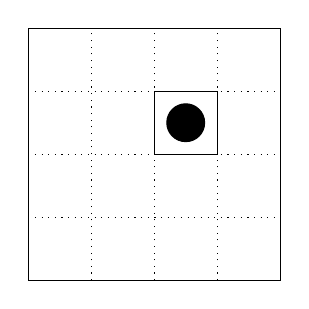
\begin{tikzpicture}[scale=0.8]
\draw[dotted] (0,0) grid (4,-4);
\draw (0,0) rectangle (4,-4);
\draw (2,-1) rectangle (3,-2);
\draw[fill] (2.5,-1.5) circle [radius=0.3cm];
\end{tikzpicture}
\caption{สวนหย่อมขนาด $2^n\times 2^n$ เมื่อ $n=2$ โดยเว้นช่องว่างไว้ให้รูปปั้นตรงกลาง}
\label{fig:courtyard-2}
\end{figure}
%
\enskip ในส่วนของพื้นที่ที่เหลือนั้น จะต้องปูกระเบื้องให้สวยงาม โดยที่กระเบื้องแต่ละชิ้นมีขนาด 3 ตารางหน่วย และมีรูปร่างคล้ายตัว L ดังรูปที่~\ref{fig:tile-shape}
%
\begin{figure}
\centering
\begin{tikzpicture}[scale=0.8]
\draw (0,0) -- (2,0) -- (2,-1) -- (1,-1) -- (1,-2) -- (0,-2) -- (0,0);
\draw[dotted] (1,0) -- (1,-1) -- (0,-1);
\end{tikzpicture}
\caption{รูปร่างของแผ่นกระเบื้องที่จะใช้ปูสวนหย่อม}
\label{fig:tile-shape}
\end{figure}
%
\enskip หาก $n=2$ เราอาจจะปูกระเบื้องได้ดังรูปที่~\ref{fig:courtyard-2-tiled}
%
\begin{figure}
\centering
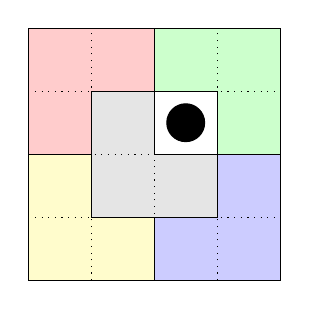
\begin{tikzpicture}[scale=0.8]
\draw[fill=red!20] (0,0) -- (2,0) -- (2,-1) -- (1,-1) -- (1,-2) -- (0,-2) -- (0,0);
\draw[fill=green!20] (2,0) -- (4,0) -- (4,-2) -- (3,-2) -- (3,-1) -- (2,-1) -- (2,0);
\draw[fill=blue!20] (4,-2) -- (4,-4) -- (2,-4) -- (2,-3) -- (3,-3) -- (3,-2) -- (4,-2);
\draw[fill=yellow!20] (0,-2) -- (0,-4) -- (2,-4) -- (2,-3) -- (1,-3) -- (1,-2) -- (0,-2);
\draw[fill=gray!20] (1,-1) -- (1,-3) -- (3,-3) -- (3,-2) -- (2,-2) -- (2,-1) -- (1,-1);

\draw[dotted] (0,0) grid (4,-4);
\draw[fill] (2.5,-1.5) circle [radius=0.3cm];
\end{tikzpicture}
\caption{วิธีการปูกระเบื้องบนสวนหย่อมในรูปที่~\ref{fig:courtyard-2}}
\label{fig:courtyard-2-tiled}
\end{figure}

ในตัวอย่างนี้ เราจะหาวิธีการปูกระเบื้องบนสวนหย่อมในลักษณะดังกล่าว รวมทั้งพิสูจน์ไปในตัวว่า วิธีการดังกล่าวนั้นถูกต้องไม่มีข้อผิดพลาด
%
\begin{theorem}
มีวิธีปูกระเบื้องรูปตัว L ลงบนสวนหย่อมขนาด $2^n\times 2^n$ ตารางหน่วย (เมื่อ $n\geq 0$) โดยเว้นช่องว่าง 1 ตารางหน่วยไว้ให้รูปปั้นตรงกลางสวนหย่อม
\begin{pf}[Failed proof]
By induction on $n$.  ให้ $P(n)\triangleq$ มีวิธีปูกระเบื้องรูปตัว L ลงบนสวนหย่อมขนาด $2^n\times 2^n$ โดยเว้นช่องว่าง 1 ตารางหน่วยไว้ให้รูปปั้นตรงกลางสวนหย่อม
\begin{itemize}
\item {\bf Base case}: ($n=0$) \quad ในกรณีนี้ สวนหย่อมมีขนาด $1\times 1$ ตารางหน่วย ซึ่งไม่เหลือพื้นที่ไว้ให้ปูกระเบื้อง ดังนั้น วิธีการปูกระเบื้องลงบนสวนหย่อมนี้ ก็คือการนั่งพักผ่อนอยู่เฉยๆ \quad\yea
\item {\bf Inductive step}: สมมุติว่ามีวิธีปูกระเบื้องรูปตัว L ลงบนสวนหย่อมขนาด $2^n\times 2^n$ โดยเว้นช่องว่าง 1 ตารางหน่วยไว้ให้รูปปั้นตรงกลางสวนหย่อม ต้องพิสูจน์ว่ามีวิธีปูกระเบื้องรูปตัว L ลงบนสวนหย่อมขนาด $2^{n+1}\times 2^{n+1}$ โดยเว้นช่องว่าง 1 ตารางหน่วยไว้ให้รูปปั้นตรงกลางสวนหย่อม ดังรูปที่~\ref{fig:courtyard-n+1}
%
\begin{figure}
\centering
\begin{tikzpicture}[scale=0.8]
\draw (0,0) rectangle (8,-8);
\draw[dotted] (4,0) -- (4,-8);
\draw[dotted] (0,-4) -- (8,-4);
\draw (4,-3.5) rectangle (4.5,-4);
\draw[fill] (4.25,-3.75) circle [radius=0.15cm];

\node at (-0.5,-4) {$2^{n+1}$};
\node at (4,-8.5) {$2^{n+1}$};
\node at (2,0.5) {$2^n$};
\node at (6,0.5) {$2^n$};
\node at (8.5,-2) {$2^n$};
\node at (8.5,-6) {$2^n$};
\end{tikzpicture}
\caption{สวนหย่อมขนาด $2^{n+1}\times 2^{n+1}$ โดยเว้นช่องว่างไว้ให้รูปปั้นตรงกลาง}
\label{fig:courtyard-n+1}
\end{figure}
%
\enskip แบ่งสวนหย่อมนี้ออกเป็นสวนหย่อมย่อยๆ 4 สวน โดยที่แต่ละสวนมีขนาด $2^n\times 2^n$ จะได้ว่า ช่องว่างที่เว้นไว้ให้รูปปั้นจะอยู่ที่มุมหนึ่งของหนึ่งในสวนหย่อมย่อยนี้ $\ldots$
\end{itemize}
ณ จุดนี้ จะเห็นว่า induction hypothesis ของเราไม่ช่วยอะไรมากนัก เพราะเรารู้เพียงว่า มีวิธีปูกระเบื้องโดยเว้นช่องว่างไว้\emph{ตรงกลาง}ของสวนหย่อม แต่สวนหย่อมย่อยที่เรากำลังพิจารณานั้นมีช่องว่างอยู่ที่มุม \enskip นั่นคือ บทพิสูจน์นี้เกิดความติดขัดขึ้นไม่สามารถไปต่อให้สำเร็จลุล่วงได้
\end{pf}

หากเกิดปัญหาในลักษณะดังกล่าว เราอาจจะต้องพิจารณาหา predicate $P(n)$ ที่เป็น induction hypothesis ใหม่ให้มีความแข็งแรง (strong) มากกว่าเดิม กล่าวคือ predicate ดังกล่าวดูเหมือนว่าจะพิสูจน์ให้เป็นจริงได้ยากขึ้น เนื่องจากฟังดูมีเงื่อนไขหรือข้อผูกมัดที่ทำให้เป็นไปได้ยากขึ้น แต่ในการพิสูจน์โดยอุปนัยนั้น หากเราใช้ induction hypothesis ที่แข็งแรงขึ้นกว่าเดิม สมมุติฐานในขั้นอุปนัยของเราก็จะมีมากขึ้นตามไปด้วย ซึ่งมักจะทำให้การพิสูจน์นั้นสำเร็จลุล่วงไปได้ง่ายขึ้นเช่นกัน

ในตัวอย่างนี้ หากเราเลือกใช้ induction hypothesis ใหม่ว่ามีวิธีปูกระเบื้องโดยที่เว้นช่องว่างสำหรับรูปปั้นไว้\emph{ที่ใดก็ได้}บนสวนหย่อม เราจะสามารถเขียนบทพิสูจน์ให้ลุล่วงไปได้ \enskip ทั้งนี้ โปรดสังเกตว่า เงื่อนไขใหม่ของเรานี้มีข้อผูกมัดมากขึ้น กล่าวคือ จากที่เคยต้องเว้นช่องว่างไว้ตรงกลางเท่านั้น กลับกลายมาเป็นต้องเว้นช่องว่างไว้ที่ใดก็ได้ ซึ่งดูเหมือนว่าการแก้ปัญหาใหม่นี้จะยากขึ้น เนื่องจากมีกรณีให้เราพิจารณามากขึ้น (กล่าวคือ มีตำแหน่งช่องว่างที่อาจจะเว้นไว้ได้มากตำแหน่งกว่าเดิม) \enskip อย่างไรก็ดี ในขั้นอุปนัยที่เราประสบปัญหาก่อนหน้านี้ แม้ว่าเงื่อนไขที่เราต้องการจะพิสูจน์จะยากขึ้น แต่สมมุติฐานที่เรามีก็มากขึ้นตามไปด้วย ซึ่งทำให้บทพิสูจน์นั้นเป็นไปได้ \enskip สุดท้ายนี้ ก่อนขึ้นบทพิสูจน์ ให้สังเกตว่า ถ้าเรามีวิธีปูกระเบื้องโดยเว้นช่องว่างไว้ที่ใดก็ได้ แล้วเราจะมีวิธีปูกระเบื้องโดยเว้นช่องว่างไว้ตรงกลาง นั่นคือ สมมุติฐานใหม่ของเราที่แข็งแรงขึ้นนั้น implies สมมุติฐานเดิมของเราที่อ่อนกว่า \enskip กล่าวอีกนัยหนึ่ง สมมุติฐานเดิมของเราเป็น\emph{กรณีพิเศษ} (special case) ของสมมุติฐานใหม่นั่นเอง
%
\begin{pf}
By induction on $n$.  ให้ $P(n)\triangleq$ มีวิธีปูกระเบื้องรูปตัว L ลงบนสวนหย่อมขนาด $2^n\times 2^n$ โดยเว้นช่องว่าง 1 ตารางหน่วยไว้ให้รูปปั้น ณ ที่ใดก็ได้ของสวนหย่อม
\begin{itemize}
\item {\bf Base case}: ($n=0$) \quad ในกรณีนี้ สวนหย่อมมีขนาด $1\times 1$ ตารางหน่วย ซึ่งไม่เหลือพื้นที่ไว้ให้ปูกระเบื้อง ดังนั้น วิธีการปูกระเบื้องลงบนสวนหย่อมนี้ ก็คือการนั่งพักผ่อนอยู่เฉยๆ \quad\yea
\item {\bf Inductive step}: สมมุติว่ามีวิธีปูกระเบื้องรูปตัว L ลงบนสวนหย่อมขนาด $2^n\times 2^n$ โดยเว้นช่องว่าง 1 ตารางหน่วยไว้ให้รูปปั้น ณ ที่ใดก็ได้ของสวนหย่อม ต้องพิสูจน์ว่ามีวิธีปูกระเบื้องรูปตัว L ลงบนสวนหย่อมขนาด $2^{n+1}\times 2^{n+1}$ โดยเว้นช่องว่าง 1 ตารางหน่วยไว้ให้รูปปั้น ณ ที่ใดก็ได้ของสวนหย่อม ดังรูปที่~\ref{fig:courtyard-n+1-general}
%
\begin{figure}
\centering
\begin{tikzpicture}[scale=0.8]
\draw (0,0) rectangle (8,-8);
\draw[dotted] (4,0) -- (4,-8);
\draw[dotted] (0,-4) -- (8,-4);
\draw (6,-1.5) rectangle (6.5,-2);
\draw[fill] (6.25,-1.75) circle [radius=0.15cm];

\node at (-0.5,-4) {$2^{n+1}$};
\node at (4,-8.5) {$2^{n+1}$};
\node at (2,0.5) {$2^n$};
\node at (6,0.5) {$2^n$};
\node at (8.5,-2) {$2^n$};
\node at (8.5,-6) {$2^n$};
\end{tikzpicture}
\caption{สวนหย่อมขนาด $2^{n+1}\times 2^{n+1}$ โดยเว้นช่องว่างไว้ให้รูปปั้นที่ใดก็ได้}
\label{fig:courtyard-n+1-general}
\end{figure}
%
\enskip แบ่งสวนหย่อมนี้ออกเป็นสวนหย่อมย่อยๆ 4 สวน โดยที่แต่ละสวนมีขนาด $2^n\times 2^n$ จะได้ว่า หนึ่งในส่วนหย่อมย่อยนี้จะมีช่องว่างที่ต้องเว้นไว้ให้รูปปั้นดังกล่าว ณ ตำแหน่งใดตำแหน่งหนึ่ง ส่วนอีก 3 สวนหย่อมย่อยที่เหลือนั้น ให้เว้นช่องว่างไว้ก่อนตรงมุมที่อยู่ตรงกลางของสวนหย่อมใหญ่ ดังรูปที่~\ref{fig:courtyard-n+1-inductive}
%
\begin{figure}
\centering
\begin{tikzpicture}[scale=0.8]
\draw (0,0) rectangle (8,-8);
\draw[dotted] (4,0) -- (4,-8);
\draw[dotted] (0,-4) -- (8,-4);
\draw (6,-1.5) rectangle (6.5,-2);
\draw[fill] (6.25,-1.75) circle [radius=0.15cm];

\node at (-0.5,-4) {$2^{n+1}$};
\node at (4,-8.5) {$2^{n+1}$};
\node at (2,0.5) {$2^n$};
\node at (6,0.5) {$2^n$};
\node at (8.5,-2) {$2^n$};
\node at (8.5,-6) {$2^n$};

\draw[fill=gray!20] (3.5,-3.5) rectangle (4,-4);
\draw[fill=gray!20] (3.5,-4) rectangle (4,-4.5);
\draw[fill=gray!20] (4,-4) rectangle (4.5,-4.5);
\end{tikzpicture}
\caption[วิธีการปูกระเบื้องบนสวนหย่อมใหญ่]{หากจะปูกระเบื้องสวนหย่อมใหญ่ ให้เว้นช่องว่างไว้ตรงมุมของสวนหย่อมย่อย 3 สวนที่ไม่ได้เว้นช่องว่างไว้ก่อนหน้านี้ จากนั้น สามารถใช้ induction hypothesis หาวิธีปูกระเบื้องสวนหย่อมย่อยได้}
\label{fig:courtyard-n+1-inductive}
\end{figure}
%
\enskip By I.H., แต่ละสวนหย่อมย่อยนี้ มีวิธีปูกระเบื้องรูปตัว L โดยเว้นช่องว่าง 1 ตารางหน่วยไว้ตามตำแหน่งที่ได้กำหนด \enskip เมื่อปูกระเบื้องสวนหย่อมย่อยเรียบร้อยแล้ว จะเหลือพื้นที่ 3 ตารางหน่วยตรงมุมของสวนหย่อมย่อยที่เราเว้นไว้ก่อนหน้านี้ที่ยังว่างอยู่ ให้นำกระเบื้องอีกแผ่นไปปูทับ ซึ่งจะปิดได้สนิทพอดี ทำให้สวนหย่อมใหญ่เหลือช่องว่างจากตอนต้นเพียงช่องเดียว ดังนั้น วิธีปูกระเบื้องดังกล่าว เว้นช่องว่างไว้ให้รูปปั้นตามที่ต้องการ
\end{itemize}

เมื่อเราได้พิสูจน์ว่ามีวิธีปูกระเบื้องโดยเว้นช่องว่างไว้ ณ ที่ใดก็ได้ของสวนหย่อมแล้ว ก็ย่อมมีวิธีปูกระเบื้องโดยเว้นช่องว่างไว้สำหรับรูปปั้นตรงกลางสวนหย่อมด้วย ดังที่เราต้องการตั้งแต่แรก เป็นอันจบบทพิสูจน์โดยครบถ้วนสมบูรณ์
\end{pf}
\end{theorem}

\subsection{Induction pitfalls}

ที่ผ่านมานั้น เราได้เห็นบทพิสูจน์โดยอุปนัยมาแล้วหลายบทพิสูจน์ ตัวอย่างต่อไปนี้จะเป็นวิธีการใช้อุปนัยที่มีข้อบกพร่อง
%
\begin{theorem}[not!]
ม้าทุกตัวมีสีเดียวกัน
\begin{pf}[False proof]
By induction. ให้ $P(n)\triangleq$ ม้า $n$ ตัวใดๆ มีสีเดียวกัน
\begin{itemize}
\item {\bf Base case}: ($n=1$) \quad ม้า $1$ ตัวใดๆ ย่อมมีสีเดียวกัน \quad\yea
\item {\bf Inductive step}: สมมุติว่าม้า $n$ ตัวใดๆ มีสีเดียวกัน \enskip พิจารณาม้า $n+1$ ตัวใดๆ \enskip หากนำม้ามาเรียงหน้ากระดาน แล้วพิจารณาเพียง $n$ ตัวแรกในลักษณะต่อไปนี้
\[
\overbrace{d_1,d_2,\ldots,d_n}^{\textup{$n$ ตัว}},d_{n+1}
\]
จาก I.H. จะได้ว่า ม้าทั้ง $n$ ตัวแรกนี้มีสีเดียวกัน กล่าวคือ หากให้ $c(d_i)$ เป็นสีของม้าตัวที่ $d_i$ จะได้ว่า \[c(d_1)=c(d_2)=\cdots=c(d_n)\] แต่ถ้าเราพิจารณาม้าเพียง $n$ ตัวหลังในลักษณะต่อไปนี้
\[
d_1,\overbrace{d_2,\ldots,d_n,d_{n+1}}^{\textup{$n$ ตัว}}
\]
จาก I.H. จะได้ว่า ม้าทั้ง $n$ ตัวหลังนี้มีสีเดียวกัน กล่าวคือ \[c(d_2)=\cdots=c(d_n)=c(d_{n+1})\]

เนื่องจาก $c(d_2)=\cdots=c(d_n)$ และ $c(d_1)=c(d_2)$ และ $c(d_n)=c(d_{n+1})$ เราสามารถสรุปได้ว่า $c(d_1)=c(d_{n+1})$ ด้วย กล่าวคือ ม้าทั้ง $n+1$ ตัวนี้มีสีเดียวกัน \quad\yea
\end{itemize}
ดังนั้น ม้าทุกตัวมีสีเดียวกัน ตามที่ต้องการ
\end{pf}

เนื่องจากในชีวิตจริง เราทราบว่า ม้าทุกตัวไม่ได้มีสีเดียวกันทั้งหมด บทพิสูจน์นี้จำเป็นต้องมีข้อผิดพลาดที่ใดที่หนึ่ง

ในขั้นอุปนัยข้างต้น เราพยายามพิสูจน์ว่า $P(n)\implies P(n+1)$ เมื่อ $n\geq 1$ \enskip หาก $n=1$ จะได้ว่า เราต้องพิสูจน์ว่า $P(1)\implies P(2)$ กล่าวคือ หากเราทราบว่าม้า 1 ตัวใดๆ มีสีเดียวกัน แล้วเราต้องพิสูจน์ว่าม้า 2 ตัวใดๆ มีสีเดียวกันด้วย \enskip แต่ถ้านำม้า 2 ตัวมาเรียงหน้ากระดาน แล้วพิจารณาเพียง 1 ตัวแรก จะได้แผนภาพในลักษณะต่อไปนี้
\[
\overbrace{d_1}^{\textup{$1$ ตัว}},d_2
\]
จาก I.H. จะได้ว่า ม้า $1$ ตัวแรกนี้มีสีเดียวกัน แต่ถ้าเราพิจารณาม้าเพียง $1$ ตัวหลัง จะได้แผนภาพในลักษณะต่อไปนี้
\[
d_1,\overbrace{d_2}^{\textup{$1$ ตัว}}
\]
จาก I.H. จะได้ว่า ม้า $1$ ตัวหลังนี้มีสีเดียวกัน

ณ จุดนี้ ยังไม่เกิดข้อผิดพลาดขึ้น แต่ในขั้นตอนต่อไป บทพิสูจน์ข้างต้นได้ให้เหตุผลว่า $c(d_2)=\cdots=c(d_n)$ แต่เนื่องจาก $n=1$ จะได้ว่าสมการดังกล่าวไม่มีม้าให้ใช้เปรียบเทียบเลยเนื่องจาก $n$ มีค่าน้อยเกินไป ดังนั้น เราไม่สามารถสรุปได้ว่า $c(d_1)=c(d_2)$ ได้ เพราะว่าไม่มีม้าตรงกลางแถวหน้ากระดานให้เราใช้เชื่อมโยงม้าตัวแรกและม้าตัวสุดท้ายว่ามีสีเดียวกัน \enskip กล่าวอีกนัยหนึ่ง ถึงแม้ว่าม้าตัวแรกจะมีสีเดียวกัน และม้าตัวที่สองจะมีสีเดียวกัน แต่สีเดียวกันที่ว่านี้อาจจะเป็นคนละสีก็ได้ ทำให้เราไม่สามารถสรุปได้แน่ชัดว่าม้าทั้งสองตัวนี้ย่อมมีสีเดียวกันด้วย

ดังนั้น บทพิสูจน์ข้างต้นมีข้อผิดพลาดเกิดขึ้นในขณะที่กำลังพิสูจน์ว่า $P(1)\implies P(2)$ เป็นจริง \enskip ทั้งนี้ หากจะปรับเปลี่ยนบทพิสูจน์ให้เริ่ม base case จาก $n=2$ จะได้ว่า ขั้นอุปนัยของเรานั้นจะถูกต้อง เนื่องจาก $P(n)\implies P(n+1)$ เมื่อ $n\geq 2$ อย่างไรก็ดี ขั้นฐานที่เราจะต้องพิสูจน์นั้นก็กลายเป็น $P(2)$ ด้วย ซึ่งมีค่าความจริงเป็นเท็จ เนื่องจากเราสามารถหาม้า 2 ตัวที่มีคนละสีได้ นั่นคือ ข้อผิดพลาดในบทพิสูจน์ที่ปรับเปลี่ยนนี้จะย้ายไปที่ base case แทน
\end{theorem}


\section{Strong induction}

\emph{การพิสูจน์โดยอุปนัยอย่างแรง} (proof by strong induction) เป็นอีกกลวิธีที่ใช้ในการพิสูจน์ว่า predicate $P(n)$ นั้นเป็นจริงสำหรับจำนวนนับ $n$ ทุกตัว โดยใช้ axiom คล้ายกับ induction

Axiom ที่จะใช้ในการพิสูจน์ มีดังนี้
\begin{axiom}[strong induction]
ให้ $P(n)$ เป็น predicate โดยที่ $n\in\mathbb{N}$ \enskip ถ้าสองเงื่อนไขต่อไปนี้เป็นจริง
\begin{enumerate}
\item $P(0)$ เป็นจริง และ
\item\label{ax:strong-ind} $\forall n\in\mathbb{N}:\left(P(0)\wedge P(1)\wedge\cdots\wedge P(n)\right)\implies P(n+1)$ เป็นจริง
\end{enumerate}
แล้ว $\forall n\in\mathbb{N}:P(n)$ จะเป็นจริงด้วย
\end{axiom}
จุดที่แตกต่างไปจาก induction axiom ก็คือสมมุติฐานในข้อที่~\ref{ax:strong-ind} ข้างต้น ซึ่งใน induction นั้นเราสามารถใช้ $P(n)$ เป็นสมมุติฐานได้เพียงอย่างเดียว แต่ใน strong induction นั้น เราสามารถใช้ $P(0),P(1),\ldots,P(n)$ เป็นสมมุติฐานได้ทั้งหมด อย่างไรก็ดี เราอาจจะไม่ได้ใช้สมมุติฐานทุกตัวที่เรามีจนครบในบทพิสูจน์ก็เป็นได้

ขั้นตอนการเขียนบทพิสูจน์โดยอุปนัยอย่างแรง เปลี่ยนแปลงไปจากขั้นตอนของ induction ดังนี้
\begin{itemize}
\item By strong induction.
\item \emph{ขั้นอุปนัย} (inductive step): ตั้งสมมุติฐานว่า $P(0),P(1),\ldots,P(n)$ เป็นจริง เพื่อใช้ในการพิสูจน์ว่า $P(n+1)$ เป็นจริง
\end{itemize}

\begin{theorem}
หากต้องการแบ่งกลุ่มให้มีสมาชิกกลุ่มละ 3 หรือ 4 คน จะมีวิธีแบ่งกลุ่มเสมอหากมีคนอย่างน้อย 6 คน
\begin{pf}
By strong induction.  ให้ $P(n)\triangleq$ มีวิธีแบ่งกลุ่มคน $n$ คน ให้มีสมาชิกกลุ่มละ 3 หรือ 4 คน
\begin{itemize}
\item {\bf Base case}: ($n=6$) \quad แบ่ง 6 คนเป็น 2 กลุ่ม กลุ่มละ 3 คน \quad\yea
\item {\bf Inductive step}: สมมุติว่ามีวิธีแบ่งกลุ่มคน $6,7,\ldots,n$ คน ต้องพิสูจน์ว่ามีวิธีแบ่งกลุ่มคน $n+1$ คน (เมื่อ $n\geq 6$)
\begin{itemize}
\item $n=6$: ต้องพิสูจน์ว่ามีวิธีแบ่งกลุ่มคน 7 คน (โดยเรารู้ว่ามีวิธีแบ่งกลุ่มคน 6 คน) \enskip แบ่งได้เป็น 2 กลุ่ม กลุ่มหนึ่งมี 3 คน อีกกลุ่มหนึ่งมี 4 คน (ในที่นี้ เราไม่ได้ใช้ I.H. แต่อย่างใด)
\item $n=7$: ต้องพิสูจน์ว่ามีวิธีแบ่งกลุ่มคน 8 คน (โดยเรารู้ว่ามีวิธีแบ่งกลุ่มคน $6,7$ คน) \enskip แบ่งได้เป็น 2 กลุ่ม กลุ่มละ 4 คน (ในที่นี้ เราไม่ได้ใช้ I.H. แต่อย่างใดเช่นกัน)
\item $n\geq 8$: ต้องพิสูจน์ว่าแบ่ง $n+1$ คนได้ (โดยรู้ว่าแบ่ง $6,7,\ldots,n$ คนได้) \enskip เนื่องจาก $n-2\geq 6$ จาก I.H. จะได้ว่า มีวิธีแบ่งกลุ่มคน $n-2$ คน \enskip ดังนั้น หากต้องการแบ่งกลุ่มคน $n+1$ คน ให้ดึง 3 คนออกมาก่อน จะเหลือ $n-2$ คน \enskip แบ่ง $n-2$ คนนี้ตาม I.H. แล้วจับ 3 คนที่ดึงออกมาอยู่กลุ่มเดียวกัน ก็จะได้วิธีแบ่งกลุ่มคน $n+1$ คน ตามที่ต้องการ \quad\yea
\end{itemize}
\end{itemize}
\end{pf}
ณ จุดนี้ อาจจะเกิดข้อสงสัยขึ้นว่า ทุกครั้งที่มีคนอย่างน้อย 8 คน เราดึงคนออกไป 3 คนเพื่อจัดเป็นกลุ่มทุกครั้ง ซึ่งดูเหมือนว่าจะไม่ค่อยมีกลุ่มที่มี 4 คนเลย อย่างไรก็ดี เราสามารถดึง 4 คนออกมาก่อนได้เช่นกัน แต่ถ้า $n=8$ เราจะยังไม่สามารถใช้ induction hypothesis ได้ เนื่องจาก $(n+1)-4=n-3$ นั้นยังน้อยเกินไป \enskip ดังนั้น หากต้องการดึง 4 คนออกมาก่อน จะต้องเขียนแยกกรณีที่ $n=8$ ออกมา กล่าวคือ ต้องแบ่งกรณีที่ $n\geq 8$ ข้างต้นออกเป็นดังต่อไปนี้
\begin{itemize}
\item $n=8$: ต้องพิสูจน์ว่ามีวิธีแบ่งกลุ่มคน 9 คน (โดยเรารู้ว่ามีวิธีแบ่งกลุ่มคน $6,7,8$ คน) \enskip แบ่งได้เป็น 3 กลุ่ม กลุ่มละ 3 คน (ในที่นี้ เราไม่ได้ใช้ I.H. แต่อย่างใดเช่นกัน)
\item $n\geq 9$: ต้องพิสูจน์ว่าแบ่ง $n+1$ คนได้ (โดยรู้ว่าแบ่ง $6,7,\ldots,n$ คนได้) \enskip เนื่องจาก $n-3\geq 6$ จาก I.H. จะได้ว่า มีวิธีแบ่งกลุ่มคน $n-3$ คน \enskip ดังนั้น หากต้องการแบ่งกลุ่มคน $n+1$ คน ให้ดึง 4 คนออกมาก่อน จะเหลือ $n-3$ คน \enskip แบ่ง $n-3$ คนนี้ตาม I.H. แล้วจับ 4 คนที่ดึงออกมาอยู่กลุ่มเดียวกัน ก็จะได้วิธีแบ่งกลุ่มคน $n+1$ คน ตามที่ต้องการ
\end{itemize}
\end{theorem}

\subsection{The unstacking game}

ในตัวอย่างนี้ จะพิจารณาเกมที่ให้แบ่งกองไม้สูง $n$ ชิ้น ออกเป็นสองกอง จากนั้น ในแต่ละกอง ให้แบ่งกองไม้ออกในลักษณะเดียวกันไปเรื่อยๆ จนกระทั่งไม่มีกองใดมีไม้มากกว่า 1 ชิ้นเลย

การคิดคะแนนในเกมนี้ จะคิดเมื่อมีการแบ่งกองไม้เกิดขึ้น โดยคะแนนในแต่ละตาคำนวณได้จากผลคูณของจำนวนชิ้นไม้ในแต่ละกองที่เพิ่งแบ่งออกมา และคะแนนรวมทั้งหมดคือผลรวมของคะแนนในแต่ละตา

ตัวอย่างเช่น หากเริ่มด้วยกองไม้ 4 ชิ้น และตาแรกแบ่งออกเป็นกองละ 2 ชิ้น จะได้ว่า คะแนนในตาแรกเป็น $2\cdot 2=4$ จากนั้น ในแต่ละกองที่แบ่งออกมาสามารถแบ่งเป็นกองละ 1 ชิ้นได้เท่านั้น โดยใช้ทั้งหมด 2 ตา จะได้ว่า ตาหนึ่งๆ ได้คะแนน $1\cdot 1=1$ ดังนั้น คะแนนรวมทั้งหมดในการเล่นวิธีนี้คือ $4+1+1=6$

\begin{theorem}
ทุกๆ กลยุทธ์ในการแบ่งกองไม้ $n$ ชิ้นจนหมด (เมื่อ $n\geq 1$) จะได้คะแนนเท่ากัน (เรียกคะแนนนี้ว่า $S(n)$)
\begin{pf}[Failed proof]
By strong induction.  ให้ $P(n)\triangleq$ ทุกๆ กลยุทธ์ในการแบ่งกองไม้ $n$ ชิ้นจนหมด จะได้คะแนน $S(n)$
\begin{itemize}
\item {\bf Base case}: ($n=1$) \quad วิธีการแบ่งกองไม้ 1 ชิ้น ย่อมมีวิธีเดียว คือ ไม่แบ่ง ดังนั้น ทุกๆ กลยุทธ์ก็ย่อมได้คะแนนเท่ากันคือ $S(0)$ \quad\yea
\item {\bf Inductive step}: สมมุติว่าทุกๆ กลยุทธ์ในการแบ่งกองไม้ $1$ ชิ้นจนหมด ได้คะแนนเท่ากันคือ $S(1)$; ทุกๆ กลยุทธ์ในการแบ่งกองไม้ $2$ ชิ้นจนหมด ได้คะแนนเท่ากันคือ $S(2)$; $\ldots$; และทุกๆ กลยุทธ์ในการแบ่งกองไม้ $n$ ชิ้นจนหมด ได้คะแนนเท่ากันคือ $S(n)$ \enskip ต้องพิสูจน์ว่า ทุกๆ กลยุทธ์ในการแบ่งกองไม้ $n+1$ ชิ้นจนหมด จะได้คะแนน $S(n+1)$

หากแบ่งกองไม้ $n+1$ ชิ้นเป็นสองกอง โดยที่กองหนึ่งมี $k$ ชิ้น จะได้ว่า อีกกองหนึ่งมี $n+1-k$ ชิ้น ดังนั้น ในตานี้ จะได้คะแนน $k(n+1-k)$ ทันที จากนั้น ต้องแบ่งกองไม้แต่ละกองไปเรื่อยๆ จนแบ่งต่อไม่ได้อีก \enskip By I.H., จะได้ว่า คะแนนรวมที่จะได้จากการแบ่งไม้ $k$ ชิ้น คือ $S(k)$ และคะแนนรวมที่จะได้จากการแบ่งไม้ $n+1-k$ ชิ้น คือ $S(n+1-k)$ ดังนั้น คะแนนรวมที่จะได้จากการแบ่งกองไม้ $n+1$ ชิ้นคือ \[S(n+1)=k(n+1-k)+S(k)+S(n+1-k)\] \ldots
\end{itemize}
\end{pf}

จะเห็นว่า เกิดการติดขัดในบทพิสูจน์ขึ้น เนื่องจากในแต่กลยุทธ์นั้น $k$ ไม่เท่ากัน เพราะเราอาจจะแบ่งกองไม้เป็นสองกองที่มีขนาดต่างๆ กัน แต่เราไม่มีวิธีการเปรียบเทียบคะแนนในแต่ละกลยุทธ์ นอกจากนี้ คะแนนในตาแรกก็ยังขึ้นกับ $k$ อีกด้วย \enskip ปัญหาที่เกิดขึ้นนี้สืบเนื่องมาจาก induction hypothesis ที่เรามีอยู่นั้นไม่แข็งแรงพอ ซึ่งมีวิธีแก้ไขคือเขียน predicate ใหม่ให้มีเงื่อนไขหรือข้อผูกมัดให้มากขึ้น \enskip ในที่นี้ หากเราหาสูตรที่คำนวณคะแนนได้ออกมาอย่างแน่ชัด ก็เพียงพอที่จะใช้พิสูจน์ได้โดยไม่ติดขัด \enskip โปรดสังเกตว่า หาก induction hypothesis พูดถึงคะแนนรวมที่คำนวณออกมาได้อย่างเฉพาะเจาะจง ก็ย่อมเกิดข้อผูกมัดที่ทำให้ induction hypothesis นั้นแข็งแรงขึ้น ซึ่งจะทำให้เราสามารถตั้งสมมุติฐานได้รัดกุมมากขึ้นด้วย และหากสามารถคำนวณคะแนนให้เฉพาะเจาะจงได้ ก็แปลว่าคะแนนที่จะได้นั้นก็ย่อมเท่ากัน ดั่งที่เราต้องการจะพิสูจน์ตั้งแต่ต้น
\end{theorem}

\begin{theorem}
ทุกๆ กลยุทธ์ในการแบ่งกองไม้ $n$ ชิ้นจนหมด (เมื่อ $n\geq 1$) จะได้คะแนนเท่ากัน คือ $S(n)=\frac{n(n-1)}{2}$
\begin{pf}
By strong induction.  ให้ $P(n)\triangleq$ ทุกๆ กลยุทธ์ในการแบ่งกองไม้ $n$ ชิ้นจนหมด จะได้คะแนน $S(n)=\frac{n(n-1)}{2}$
\begin{itemize}
\item {\bf Base case}: ($n=1$) \quad วิธีการแบ่งกองไม้ 1 ชิ้น ย่อมมีวิธีเดียว คือ ไม่แบ่ง ซึ่งไม่ได้คะแนน และเราต้องการพิสูจน์ว่า ทุกๆ กลยุทธ์ก็ย่อมได้คะแนนเท่ากันคือ $S(0)=\frac{0(1-0)}{2}=0$ ซึ่งถูกต้อง \quad\yea
\item {\bf Inductive step}: สมมุติว่าทุกๆ กลยุทธ์ในการแบ่งกองไม้ $k$ ชิ้นจนหมด โดยที่ $1\leq k\leq n$ จะได้คะแนนเท่ากันคือ $S(k)=\frac{k(k-1)}{2}$ \enskip ต้องพิสูจน์ว่า ทุกๆ กลยุทธ์ในการแบ่งกองไม้ $n+1$ ชิ้นจนหมด จะได้คะแนน $S(n+1)=\frac{(n+1)n}{2}$

หากแบ่งกองไม้ $n+1$ ชิ้นเป็นสองกอง โดยที่กองหนึ่งมี $k$ ชิ้น จะได้ว่า อีกกองหนึ่งมี $n+1-k$ ชิ้น ดังนั้น ในตานี้ จะได้คะแนน $k(n+1-k)$ ทันที จากนั้น ต้องแบ่งกองไม้แต่ละกองไปเรื่อยๆ จนแบ่งต่อไม่ได้อีก \enskip By I.H., จะได้ว่า ไม่ว่าจะใช้กลยุทธ์ใดก็ตาม คะแนนรวมที่จะได้จากการแบ่งไม้ $k$ ชิ้น คือ $S(k)=\frac{k(k-1)}{2}$ และคะแนนรวมที่จะได้จากการแบ่งไม้ $n+1-k$ ชิ้น คือ $S(n+1-k)=\frac{(n+1-k)(n-k)}{2}$ (สังเกตว่า $k$ และ $n+1-k$ ทั้งคู่นั้นมีค่าอย่างน้อย 1 และอย่างมาก $n$ ซึ่งตรงตามเงื่อนไขของ I.H. ที่เราสมมุติไว้) ดังนั้น คะแนนรวมที่จะได้จากการแบ่งกองไม้ $n+1$ ชิ้นคือ
\begin{align*}
S(n+1)
&=k(n+1-k)+S(k)+S(n+1-k) \\
&=k(n+1-k)+\frac{k(k-1)}{2}+\frac{(n+1-k)(n-k)}{2} \\
&=(n+1-k)\left[k+\frac{(n-k)}{2}\right]+\frac{k(k-1)}{2} \\
&=(n+1-k)\left[\frac{n+k}{2}\right]+\frac{k(k-1)}{2} \\
&=\frac{((n+1)-k)(n+k)}{2}+\frac{k(k-1)}{2} \\
&=\frac{(n+1)n-kn+k(n+1)-k^2+k(k-1)}{2} \\
&=\frac{(n+1)n-kn+kn+k-k^2+k^2-k}{2} \\
&=\frac{(n+1)n}{2} \quad\textup{\yea}
\end{align*}
\end{itemize}
\end{pf}
\end{theorem}

\subsection{Induction vs strong induction}
ในการพิสูจน์โดยอุปนัยอย่างแรงนั้น สมมุติฐานที่เรามีในขั้นอุปนัย (inductive step) นั้นมีมากกว่าในการพิสูจน์โดยอุปนัย \enskip จากข้อเท็จจริงนี้ เราสามารถสรุปได้ว่า หากเราสามารถใช้ induction พิสูจน์ประพจน์หนึ่งๆ ได้ ก็ย่อมสามารถใช้ strong induction พิสูจน์ได้เช่นกัน \enskip แต่ในทางกลับกัน หากเราสามารถใช้ strong induction พิสูจน์ประพจน์หนึ่งๆ ได้ แล้วเราจะสามารถใช้ induction พิสูจน์ประพจน์นั้นๆ ได้หรือไม่

หากพิจารณาโดยผิวเผิน อาจจะเห็นว่า การพิสูจน์โดยอุปนัยอย่างแรงนั้นน่าจะทำให้เราเขียนบทพิสูจน์ได้มากกว่าเดิม กล่าวคือ อาจจะมี propositions บางตัวที่เราไม่สามารถพิสูจน์โดยใช้ induction ได้ แต่สามารถพิสูจน์โดยใช้ strong induction ได้ อย่างไรก็ดี strong induction นั้นไม่ทำให้เราพิสูจน์ได้มากขึ้นแต่อย่างใด แต่เป็นเพียงเครื่องมืออำนวยความสะดวกให้เราเขียนบทพิสูจน์ได้รวดเร็วและกระชับยิ่งขึ้น \enskip กล่าวอีกนัยหนึ่ง หากใช้ strong induction พิสูจน์อะไรได้ ก็สามารถใช้ induction พิสูจน์ได้เช่นเดียวกัน แต่บทพิสูจน์ที่ใช้ induction นั้นอาจจะมีความซับซ้อนมากกว่า ดังที่จะได้สาธิตต่อไปนี้

ในการพิสูจน์โดยใช้ strong induction นั้น เราต้องการพิสูจน์ว่า predicate $P(n)$ หนึ่งๆ นั้นเป็นจริงสำหรับทุกค่า $n\in\mathbb{N}$ โดยใน inductive step เรามีสมมุติฐานคือ $\forall n'\leq n: P(n')$ \enskip เราจะแปลงบทพิสูจน์นี้เป็นบทพิสูจน์โดยใช้ induction โดยจะพิสูจน์ predicate $Q(n)\triangleq\forall n'\leq n: P(n')$ ว่าเป็นจริงสำหรับทุกค่า $n\in\mathbb{N}$
\begin{itemize}
\item {\bf Base case}: ($n=0$) \quad ต้องพิสูจน์ว่า $Q(0)$ เป็นจริง กล่าวคือ $\forall n'\leq 0: P(n')$ ซึ่งมี $n'$ เพียงค่าเดียวที่เป็นไปได้คือ $0$ \enskip ดังนั้น ในการพิสูจน์ว่า $Q(0)$ เป็นจริง จึงใช้บทพิสูจน์เดียวกันกับการแสดงว่า $P(0)$ เป็นจริงในบทพิสูจน์โดยใช้ strong induction ที่เรามีอยู่เดิม
\item {\bf Inductive step}: ในขั้นตอนนี้ เราต้องพิสูจน์ว่า $Q(n+1)$ เป็นจริง โดยสมมุติฐานที่เรามีคือ $Q(n)$ ซึ่งแปลว่า $\forall n'\leq n: P(n')$ กล่าวคือ $P(0),P(1),\ldots,P(n)$ เป็นจริง \enskip ดังนั้น หากจะพิสูจน์ว่า $Q(n+1)$ เป็นจริง กล่าวคือ $\forall n'\leq n+1: P(n')$ เราจึงต้องพิสูจน์ว่า $P(n+1)$ เป็นจริง (เนื่องจากเราทราบว่า $P(0),\ldots,P(n)$ เป็นจริงอยู่แล้วจากสมมุติฐาน) ซึ่งเราสามารถใช้บทพิสูจน์เดียวกันกับการแสดงว่า $P(n+1)$ เป็นจริงในบทพิสูจน์โดยใช้ strong induction ที่เรามีอยู่เดิม
\end{itemize}
ดังนั้น บทพิสูจน์ข้างต้นจึงเป็นบทพิสูจน์ที่ใช้วิธี induction แต่สามารถพิสูจน์ประพจน์ที่พิสูจน์ได้โดยวิธี strong induction ซึ่งแปลว่าวิธี strong induction นั้นไม่ได้ทำให้เราสามารถพิสูจน์ประพจน์ได้จำนวนมากขึ้นกว่าเดิมแต่อย่างใด

\section{Loop invariants}
ในงานด้านวิศวกรรมคอมพิวเตอร์นั้น การเขียนโปรแกรมเป็นสิ่งที่หลีกเลี่ยงไม่ได้ \enskip แต่เมื่อเราเขียนโปรแกรมแล้ว เราจะมั่นใจได้อย่างไรว่าโปรแกรมที่เขียนขึ้นมานั้นทำงานได้ถูกต้องตามความต้องการ

\begin{example}\label{ex:prog-sum}
โปรแกรมพื้นฐานต่อไปนี้ใช้หาผลรวมของเลขจำนวนเต็มตั้งแต่ $1$ ถึง $n$
\begin{lstlisting}[language=java]
int sum = 0;
for (int i = 1; i <= n; i++)
  sum += i;
\end{lstlisting}
แต่เราจะทราบได้อย่างไรว่า ผลลัพธ์สุดท้าย (\cd{sum}) ของโปรแกรมนี้จะเป็นค่าที่เราต้องการเสมอ กล่าวคือ จะมั่นใจได้อย่างไรว่า \cd{sum} จะเป็นผลรวมของเลขจำนวนเต็มตั้งแต่ $1$ ถึง $n$
\end{example}

\begin{example}\label{ex:prog-insertion-sort}
โปรแกรมต่อไปนี้เรียงลำดับสมาชิกใน array จากน้อยไปมาก
\begin{lstlisting}[language=java]
int[] a = ...;
int n = a.length;
for (int i = 1; i < n; i++) {
  int x = a[i];
  int j = i;
  for (; j > 0 && a[j-1] > x; j--)
    a[j] = a[j-1];
  a[j] = x;
}
\end{lstlisting}
หากเราได้เรียนรู้วิธีการเรียงลำดับแบบต่างๆ มาก่อน เราจะเห็นทันทีว่าโปรแกรมข้างต้นนั้นเป็นการเรียงลำดับแบบ \emph{insertion sort} \enskip แต่ถ้าเราไม่เคยเห็นโปรแกรมที่เขียนในลักษณะนี้มาก่อน จะแน่ใจได้อย่างไรว่าสมาชิกใน array ที่ผ่านโปรแกรมนี้มาแล้วจะเรียงลำดับจากน้อยไปมาก \enskip หากจะกล่าวให้กว้างขึ้น เราจะมั่นใจได้อย่างไรว่าโปรแกรมที่เราไม่เคยเห็นมาก่อน แต่ถูกอ้างว่าเป็นโปรแกรมที่สามารถเรียงลำดับสมาชิกใน array ได้นั้นจะทำงานได้ถูกต้องจริงๆ
\end{example}

โดยทั่วไปแล้ว โปรแกรมส่วนใหญ่มักจะใช้\emph{วงวน} (loop) ในการทำงาน \enskip หากเราสามารถให้เหตุผลในการอธิบายการทำงานของ loops ต่างๆ ในโปรแกรมได้ จะทำให้เราสามารถสรุปได้ว่าโปรแกรมที่เรากำลังพิจารณาอยู่นั้นทำงานได้ถูกต้องตามความต้องการหรือไม่ \enskip การให้เหตุผลในการทำงานของ loop นั้นสามารถทำได้โดยการเขียนประพจน์หนึ่งๆ ที่จะเป็นจริงตลอดเวลา ไม่ว่า loop จะทำงานไปแล้วกี่ครั้งก็ตาม

\begin{definition}
\emph{ตัวยืนยงของวงวน} (loop invariant) เป็นประพจน์ที่เป็นจริงเสมอ ทั้งก่อน ระหว่าง และหลังการทำงานของ loop
\end{definition}
%
\begin{example}\label{ex:prog-sum-inv}
จาก Example~\ref{ex:prog-sum} เราสามารถเขียน loop invariant ได้ว่า ก่อนการทำงานในแต่ละรอบของ loop ทั้ง $\cd{sum}=\sum_{k=1}^{\cd{i}-1}{k}$ และ $1\leq\cd{i}\leq\cd{n}+1$ เป็นจริงทั้งคู่
\end{example}

อย่างไรก็ดี loop invariants ที่เราเขียนนั้นย่อมไม่มีประโยชน์ หากเราไม่สามารถแสดงได้ว่าเป็นจริงดังอ้าง \enskip ดังนั้น เราจึงจำเป็นต้องตรวจสอบว่า loop invariants เป็นจริง โดยมีขั้นตอนหลักๆ ดังนี้
\begin{enumerate}
\item การตั้งต้น (establishment/initialization): แสดงว่า loop invariant เป็นจริงก่อนที่ loop จะเริ่มทำงาน
\item การสงวนรักษา (preservation/maintenance): แสดงว่า loop invariant เป็นจริงหลังจากจบการทำงานในแต่ละรอบของ loop
\item การตรวจสอบเงื่อนไขหลังการทำงาน (postcondition): แสดงว่า loop จะให้ผลลัพธ์ตามที่เราต้องการหากเราสมมุติว่า loop จบการทำงาน
\item การจบการทำงาน (termination): แสดงว่า loop จะจบการทำงานเสมอ
\end{enumerate}
เราจะใช้ Example~\ref{ex:prog-sum-inv} ในการสาธิตการให้เหตุผลในแต่ละขั้นตอนข้างต้น

\subsection{Establishment}
ในขั้นตอนนี้ เราต้องแสดงว่า loop invariant เป็นจริงหลังจากกำหนดค่าตั้งต้นของ loop แล้ว แต่ก่อนที่ loop จะเริ่มทำงาน \enskip ในตัวอย่างโปรแกรมที่กำลังพิจารณานั้น จุดที่เราจะพิจารณาคือหลังจากการกำหนดค่าตั้งต้น \cd{i=1} ใน \lstinline[language=Java]{for} loop แล้ว

จากโปรแกรมตัวอย่าง ก่อน loop ทำงานครั้งแรก จะได้ว่า $\cd{i}=1$ และ $\cd{sum}=0$ ดังนั้น
\[\sum_{k=1}^{\cd{i}-1}{k}=\sum_{k=1}^{1-1}{k}=\sum_{k=1}^{0}{k}=0=\cd{sum}\]
และ $1\leq\cd{i}\leq\cd{n}+1$ จึงสรุปได้ว่า loop invariant เป็นจริงก่อนการทำงานของ loop

\subsection{Preservation}
ในขั้นตอนนี้ เราต้องแสดงว่า หาก loop invariant เป็นจริงก่อนการทำงานของ loop ในรอบใดๆ แล้ว loop invariant จะยังเป็นจริงอยู่หลังจากจบการทำงานในรอบนั้นๆ ของ loop ซึ่งรวมไปถึงการปรับค่าต่างๆ เมื่อจบการทำงานในรอบนั้นๆ แล้วด้วย \enskip ในตัวอย่างโปรแกรมที่กำลังพิจารณาอยู่นั้น จุดที่เราจะพิจารณาคือหลังจากการเปลี่ยนค่า \cd{i} ด้วยคำสั่ง \cd{i++} ใน \lstinline[language=java]{for} loop แล้ว

จากโปรแกรมตัวอย่าง สมมุติว่า loop invariant เป็นจริงก่อนการทำงานในรอบถัดไป กล่าวคือ $\cd{i}\leq\cd{n}$ (เนื่องจาก loop จะทำงาน) และ
\[\cd{sum}=\sum_{k=1}^{\cd{i}-1}{k} \textup{\quad และ \quad} 1\leq\cd{i}\leq\cd{n}+1\]
เราต้องแสดงว่า หลัง loop จบการทำงานในรอบถัดไปนี้แล้ว loop invariant จะยังเป็นจริงดังเดิม โดยจะต้องพิจารณาค่าต่างๆ ที่เปลี่ยนไปเนื่องจากการทำงานของแต่ละคำสั่งใน loop

ก่อนอื่น เนื่องจากเราทราบว่า $\cd{i}\leq\cd{n}$ และ $1\leq\cd{i}\leq\cd{n}+1$ จะได้ว่า $1\leq\cd{i}\leq\cd{n}$ ก่อนการทำงานของ loop ในรอบนี้

เมื่อทำคำสั่ง \cd{sum += i} ค่าของ \cd{sum} จะเปลี่ยนเป็น $\cd{sum}'$ โดยที่
\[\cd{sum}'=\cd{sum}+\cd{i}=\left[\sum_{k=1}^{\cd{i}-1}{k}\right]+\cd{i}=\sum_{k=1}^{\cd{i}}{k}\]
จากนั้น เมื่อคำสั่ง \cd{i++} ทำงาน ค่าของ \cd{i} จะเปลี่ยนเป็น $\cd{i}'=\cd{i}+1$ กล่าวคือ $\cd{i}=\cd{i}'-1$ \enskip ดังนั้น หลังจบการทำงานของ loop ในรอบนี้ ค่าของ \cd{sum}, \cd{i}, และ \cd{n} จะเปลี่ยนไปเป็น $\cd{sum}', \cd{i}', \cd{n}'$ ตามลำดับ โดยที่ $\cd{n}'=\cd{n}$ (กล่าวคือ \cd{n} นั้นไม่เปลี่ยนค่า) และค่าอื่นๆ เป็นไปดังก่อนหน้านี้ \enskip จะได้ว่า
\[\cd{sum}'=\sum_{k=1}^{\cd{i}}{k}=\sum_{k=1}^{\cd{i}'-1}{k}\]
นอกจากนี้ เนื่องจาก $1\leq\cd{i}\leq\cd{n}$ จะได้ว่า $1\leq\cd{i}+1\leq\cd{n}+1$ กล่าวคือ $1\leq\cd{i}'\leq\cd{n}'+1$ \enskip จึงสรุปได้ว่า loop invariant นั้นยังคงเป็นจริงหลังจากการทำงานของ loop ในรอบที่ผ่านมา

ในลำดับการให้เหตุผลข้างต้น ชื่อตัวแปรต่างๆ นั้นจะเปลี่ยนแปลงเล็กน้อยเมื่อมีการเปลี่ยนแปลงค่า เพื่อป้องกันความสับสนที่อาจจะเกิดขึ้นหากตัวแปรแต่ละตัวสามารถเป็นได้หลายค่า ตัวอย่างเช่น ค่าของตัวแปร \cd{sum} นั้นเป็นค่าหนึ่งก่อนที่ loop จะเริ่มการทำงาน แต่เปลี่ยนเป็นอีกค่าหนึ่งเมื่อ loop จบการทำงาน ด้วยเหตุนี้ ชื่อของตัวแปรดังกล่าวจึงเปลี่ยนเป็น $\cd{sum}'$ เพื่อป้องกันความสับสนว่า ณ ขณะหนึ่งๆ เรากำลังกล่าวถึงตัวแปรในขั้นตอนใดของ loop \enskip อย่างไรก็ดี จะเห็นว่า เมื่อ loop จบการทำงานแล้ว ค่าสุดท้ายของแต่ละตัวแปรก็ยังคงทำให้ loop invariant เป็นจริงเช่นเดิม

นอกจากนี้ สังเกตว่า ในขั้นตอน establishment และ preservation นั้น วิธีการให้เหตุผลจะมีความใกล้เคียงกับการพิสูจน์โดยอุปนัย \enskip โดยขั้นตอน establishment นั้นเทียบเคียงได้กับ base case และขั้นตอน preservation นั้นเทียบเคียงได้กับ inductive step \enskip จะเห็นว่า เมื่อเราให้เหตุผลในสองขั้นตอนนี้เรียบร้อยแล้ว เราสามารถสรุปได้ว่า ไม่ว่า loop จะทำงานไปกี่รอบก็ตาม loop invariant ก็จะยังเป็นจริงไม่เปลี่ยนแปลง

\subsection{Postcondition}
ในขั้นตอนนี้ เราต้องแสดงว่า หาก loop invariant เป็นจริง แต่ loop นั้นไม่ทำงานในรอบต่อไปเนื่องจากเงื่อนไขควบคุม (loop guard) กลายเป็นเท็จ แล้ว loop invariant จะให้ผลลัพธ์จากการทำงานของโปรแกรมที่เราคาดหวังไว้ \enskip ในตัวอย่างโปรแกรมที่กำลังพิจารณาอยู่นั้น ผลลัพธ์ที่เราต้องการก็คือ ค่าของตัวแปร \cd{sum} ต้องเป็นผลรวมของเลขจำนวนเต็มตั้งแต่ $1$ ถึง $n$

จากโปรแกรมตัวอย่าง สมมุติว่า loop invariant เป็นจริง กล่าวคือ
\[\cd{sum}=\sum_{k=1}^{\cd{i}-1}{k} \textup{\quad และ \quad} 1\leq\cd{i}\leq\cd{n}+1\]
แต่ loop นั้นไม่ทำงานในรอบต่อไป แสดงว่า loop guard (\cd{i <= n}) นั้นเป็นเท็จ กล่าวคือ $\cd{i}>\cd{n}$ \enskip แต่เนื่องจากเราทราบว่า $1\leq\cd{i}\leq\cd{n}+1$ จึงสรุปได้ว่า ค่าของตัวแปร $\cd{i}$ นั้นเป็นได้เพียง $\cd{n}+1$ เท่านั้น \enskip หากเรานำค่านี้ไปแทนใน loop invariant ที่กล่าวถึงตัวแปร \cd{sum} จะได้ว่า
\[\cd{sum}=\sum_{k=1}^{(\cd{n}+1))-1}{k}=\sum_{k=1}^{\cd{n}}{k}\]
ซึ่งเป็นผลลัพธ์ที่เราต้องการจากการทำงานของโปรแกรม

สังเกตว่า ขั้นตอนนี้ไม่ได้แสดงว่า loop จะจบการทำงาน แต่แสดงเพียงว่า \emph{หาก} loop จบการทำงาน แล้วผลลัพธ์ที่ได้จะเป็นไปตามที่เราต้องการ \enskip ในขั้นตอนถัดไป เราจะแสดงว่า loop นั้นจบการทำงานเสมอ ซึ่งเมื่อนำผลดังกล่าวมารวมกับขั้นตอนนี้ จะทำให้เราสรุปได้ว่า loop นั้นให้ผลลัพธ์ที่ถูกต้องเสมอ

\subsection{Termination}
ในขั้นตอนสุดท้าย เราต้องแสดงว่า หาก loop invariant เป็นจริงก่อนการทำงานในแต่ละรอบของ loop แล้วในท้ายที่สุด loop ต้องจบการทำงาน โดยกำหนดค่าค่าหนึ่งที่ขึ้นกับตัวแปรต่างๆ ที่ปรากฏใน loop invariant (เรียกค่านี้ว่า $d$) ซึ่งจะใช้บ่งชี้เวลาที่ loop นี้ยังมีเหลืออยู่ในการทำงาน กล่าวคือ ค่านี้ต้องลดลงหลังแต่ละรอบของ loop จบการทำงาน และค่านี้จะลดลงไปตลอดกาลไม่ได้ นั่นคือ ต้องมีค่าคงที่ $d_0$ ที่หาก $d<d_0$ เมื่อใดแล้ว loop guard จะต้องเป็นเท็จ (ซึ่งทำให้ loop จบการทำงาน ไม่เป็น infinite loop)

จากโปรแกรมตัวอย่าง พิจารณาค่าของ $d\triangleq\cd{n}-\cd{i}$ \enskip เนื่องจากในแต่ละรอบของ loop ค่าของ \cd{i} เมื่อจบการทำงานคือ $\cd{i}'=\cd{i}+1$ ดังนั้น $d'=\cd{n}'-\cd{i}'=\cd{n}-i-1<\cd{n}-\cd{i}=d$ กล่าวคือ ค่านี้จะลดลงเสมอหลังการทำงานแต่ละรอบของ loop \enskip นอกจากนี้ พิจารณา $d_0\triangleq 0$ \enskip จะเห็นว่า $\cd{n}-\cd{i}\geq 0$ (นั่นคือ $d\geq d_0$) เสมอ มิฉะนั้น หาก $\cd{n}-\cd{i}<0$ กล่าวคือ $\cd{i}>\cd{n}$ แล้ว loop guard จะต้องเป็นเท็จ ซึ่งแปลว่า loop ดังกล่าวจะจบการทำงานนั่นเอง

\begin{example}
ในตัวอย่างนี้ เราจะทำการพิสูจน์ความถูกต้องของ insertion sort ใน Example~\ref{ex:prog-insertion-sort} \enskip ก่อนอื่น เนื่องจากโปรแกรมนี้ประกอบไปด้วย loop สองชั้น เราจึงต้องหา loop invariant สำหรับแต่ละ loop ก่อน ดังนี้

สำหรับ loop นอกนั้น ก่อนการทำงานแต่ละรอบของ loop จะได้ว่า
\begin{itemize}
\item $1\leq\cd{i}\leq\cd{n}$
\item $\cd{a}[0..\cd{i}-1]$ มีสมาชิกเช่นเดียวกับ $\cd{a}[0..\cd{i}-1]$ ก่อนเริ่มการทำงานของ loop แต่จะเรียงลำดับจากน้อยไปมาก (sorted)
\end{itemize}

สำหรับ loop ในนั้น ก่อนการทำงานแต่ละรอบของ loop จะได้ว่า
\begin{itemize}
\item $0\leq\cd{j}\leq\cd{i}$
\item $\forall k\in[\cd{j}..\cd{i}]: \cd{a}[k]\geq\cd{x}$
\item $\cd{a}[0..\cd{j}-1]$ มีสมาชิกเช่นเดียวกับ $\cd{a}[0..\cd{j}-1]$ ก่อนเริ่มการทำงานของ loop แต่จะเรียงลำดับจากน้อยไปมาก (sorted)
\item $\cd{a}[\cd{j}+1..\cd{i}]$ มีสมาชิกเช่นเดียวกับ $\cd{a}[\cd{j}..\cd{i}-1]$ ก่อนเริ่มการทำงานของ loop แต่จะเรียงลำดับจากน้อยไปมาก (sorted)
\end{itemize}

ข้อสังเกตที่สำคัญในขั้นตอนนี้คือ การหา loop invariant นั้นโดยปกติแล้วไม่ใช่กระบวนการที่ง่ายดาย แต่อาจจะต้องลองผิดลองถูกเพื่อค้นหาข้อมูลที่เพียงพอที่จะทำให้เราสามารถสรุปได้ว่าการทำงานของ loop จะยังทำให้คุณสมบัติที่เราค้นหามานั้นเป็นจริงดังเดิม \enskip ทั้งนี้ การทดลองว่า loop invariant ที่เราตั้งขึ้นมานั้นเพียงพอต่อการพิสูจน์หรือไม่ ก็คือการลองเขียนบทพิสูจน์ตามกระบวนการทั้ง 4 ขั้นตอนข้างต้น แล้วพิจารณาว่ามีส่วนใดที่ขาดหายไปหรือไม่ \enskip หากมี เราสามารถเพิ่มเข้าไปใน loop invariant ที่เราพยายามจะแสดง จนกว่าการให้เหตุผลของเราจะสำเร็จลุล่วง

ในลำดับถัดไป จะแสดงว่า loop invariant สำหรับ loop นอกนั้นเป็นจริง
\begin{itemize}
\item {\bf Establishment}: เริ่มแรก $\cd{i}=1$ ดังนั้น $1\leq\cd{i}\leq\cd{n}$ \enskip นอกจากนี้ $\cd{a}[0..1-1]=\cd{a}[0]$ นั้นเรียงตามลำดับ เนื่องจากมีสมาชิกเพียงตัวเดียว \qquad\yea

\item {\bf Preservation}: สมมุติว่า $1\leq\cd{i}\leq\cd{n}$ และ $\cd{a}[0..\cd{i}-1]$ sorted และให้ loop ทำงานในรอบต่อไป กล่าวคือ $\cd{i}<\cd{n}$ \enskip ดังนั้น $1\leq\cd{i}<\cd{n}$

เมื่อ inner loop จบการทำงาน loop invariant ของ inner loop นั้นกล่าวว่า ค่าสุดท้ายของ $\cd{j}$ จะต้องมีคุณสมบัติดังนี้ $0\leq\cd{j}\leq\cd{i}$ และ $\forall k\in[\cd{j}..\cd{i}]: \cd{a}[k]\geq\cd{x}$ \enskip นอกจากนี้ $\cd{a}[0..\cd{j}-1]$ และ $\cd{a}[\cd{j}+1..\cd{i}]$ ยัง sorted โดยที่สมาชิกใน $\cd{a}[\cd{j}+1..\cd{i}]$ นั้นเป็นเช่นเดียวกับสมาชิกของ $\cd{a}[\cd{j}..\cd{i}-1]$ ก่อนการทำงานของ inner loop อีกด้วย

เนื่องจาก inner loop จบการทำงาน แสดงว่า inner loop guard (\cd{j > 0 && a[j-1] > x}) ต้องเป็นเท็จ กล่าวคือ $\cd{j}\leq 0\vee\cd{a}[\cd{j}-1]\leq\cd{x}$ ต้องเป็นจริง \enskip แยกกรณีดังนี้
\begin{itemize}
\item $\cd{j}\leq 0$: เนื่องจาก $0\leq\cd{j}\leq\cd{i}$ จะได้ว่า $\cd{j}=0$ กล่าวคือ $\cd{a}[1..\cd{i}]$ sorted และมีสมาชิกเช่นเดียวกับ $\cd{a}[0..\cd{i}-1]$ ก่อนการทำงานของ loop \enskip นอกจากนี้ เนื่องจากเราทราบว่า $\forall k\in[0..\cd{i}]: \cd{a}[k]\geq\cd{x}$ กล่าวคือ สมาชิก $\cd{i}+1$ ตัวแรกของ \cd{a} นั้นมีค่าไม่น้อยกว่า $\cd{x}$ ทั้งสิ้น เมื่อทำคำสั่ง \cd{a[j] = x} (นั่นคือ \cd{a[0] = x}) จะได้ว่า $\cd{a}[0..\cd{i}]$ sorted และมีสมาชิกเช่นเดียวกับ $\cd{a}[0..\cd{i}]$ ก่อนการทำงานของ loop ด้วย \enskip ดังนั้น เมื่อกำหนดค่าในช่องแรกของ \cd{a} ให้เป็น \cd{x} จะได้ว่าสมาชิก $\cd{i}+1$ ตัวแรกของ \cd{a} ก็ยังคงเรียงลำดับเหมือนเดิม

\item $\cd{a}[\cd{j}-1]\leq\cd{x}$: เนื่องจาก $\cd{a}[0..\cd{j}-1]$ และ $\cd{a}[\cd{j}+1..\cd{i}]$ นั้น sorted จะได้ว่า $\forall k<\cd{j}: \cd{a}[k]\leq x$ กล่าวคือ ทุกช่องของ \cd{a} ทางด้านซ้ายของตำแหน่ง \cd{j}    จะมีค่าไม่เกิน \cd{x} และ $\forall k\in[\cd{j}..\cd{i}]: \cd{a}[k]\geq x$ กล่าวคือ ทุกช่องของ \cd{a} ทางด้านขวาของตำแหน่ง \cd{j} แต่ไม่เกินตำแหน่ง \cd{i} จะมีค่าไม่น้อยกว่า \cd{x} \enskip หากเขียนเป็นแผนภาพ จะได้ดังนี้
\begin{center}
\begin{tikzpicture}
\node[draw] (left) [minimum height=2ex,minimum width=4cm] {};
\node[below=0in of left.south west] {0};
\node[below=0in of left.south] {\small $\leq\cd{x}$, sorted};
\node[below=0in of left.south east] {$\cd{j}-1$};

\node[draw,right=1.5cm of left] (mid) [minimum height=2ex,minimum width=1em] {};
\node[below=0in of mid.south] {$\cd{j}$};

\node[draw,right=1.5cm of mid] (right) [minimum height=2ex,minimum width=4cm] {};
\node[below=0in of right.south west] {$\cd{j}+1$};
\node[below=0in of right.south] {\small $\geq\cd{x}$, sorted};
\node[below=0in of right.south east] {\cd{i}};
\end{tikzpicture}
\end{center}
เมื่อทำคำสั่ง \cd{a[j] = x} จะได้ว่า $\cd{a}[0..\cd{i}]$ sorted และมีสมาชิกเช่นเดียวกับ $\cd{a}[0..\cd{i}]$ ก่อนการทำงานของ loop
\end{itemize}
ดังนั้น ไม่ว่าในกรณีใดๆ จะได้ว่า $\cd{a}[0..\cd{i}]$ จะมีสมาชิกเช่นเดิม แต่เรียงลำดับเสมอ \enskip นอกจากนี้ เมื่อเพิ่มค่า \cd{i} ในคำสั่ง \cd{i++} จะได้ว่า $\cd{i}'=\cd{i}+1$ \enskip ดังนั้น $\cd{a}[0..\cd{i}'-1]$ นั้น sorted และเนื่องจาก $1\leq\cd{i}<\cd{n}$ จะได้ว่า $1\leq\cd{i}+1\leq\cd{n}$ กล่าวคือ $1\leq\cd{i}'\leq\cd{n}$ นั่นเอง ซึ่งแปลว่า loop invariant ยังคงเป็นจริงหลังการทำงานของ outer loop ในรอบนี้ \qquad\yea

\item {\bf Postcondition}: สมมุติว่า loop invariant เป็นจริง แต่ loop ไม่ทำงานในรอบต่อไป แสดงว่า loop guard (\cd{i < n}) เป็นเท็จ นั่นคือ $\cd{i}\geq\cd{n}$ \enskip แต่เนื่องจาก loop invariant เป็นจริง แสดงว่า $1\leq\cd{i}\leq\cd{n}$ \enskip ดังนั้น ค่าเดียวของ \cd{i} ที่เป็นไปได้คือ $\cd{i}=\cd{n}$ \enskip และจาก loop invariant เราทราบด้วยว่า $\cd{a}[0..\cd{i}-1]$ นั้น sorted จะได้ว่า $\cd{a}[0..\cd{n}-1]$ นั้น sorted กล่าวคือ array ที่เรามีอยู่นั้นเรียงลำดับได้ถูกต้องนั่นเอง \qquad\yea

\item {\bf Termination}: พิจารณา $d\triangleq\cd{n}-\cd{i}$ และ $d_0\triangleq 1$ \enskip เนื่องจากในแต่ละรอบ $\cd{i}'=\cd{i}+1$ แสดงว่า $\cd{n}'-\cd{i}'=\cd{n}-\cd{i}-1<\cd{n}-\cd{i}$ กล่าวคือ ค่าของ $d$ นั้นจะลดลงในแต่ละรอบ \enskip นอกจากนี้ $\cd{n}-\cd{i}\geq 1$ เสมอ \enskip หาก $\cd{n}-\cd{i}<1$ แสดงว่า $\cd{i}+1>\cd{n}$ กล่าวคือ $\cd{i}\geq\cd{n}$ ซึ่งจะทำให้ outer loop guard เป็นเท็จ \enskip ดังนั้น insertion sort จะจบการทำงานเสมอ \qquad\yea
\end{itemize}

ในลำดับสุดท้าย จะแสดงว่า loop invariant สำหรับ loop ในนั้นเป็นจริง
\begin{itemize}
\item {\bf Establishment}: เริ่มแรก $\cd{j}=\cd{i}$ ดังนั้น $0\leq\cd{j}\leq\cd{i}$ และเนื่องจาก outer loop invariant เป็นจริง $\cd{a}[0..\cd{i}-1]$ sorted ซึ่งแปลว่า $\cd{a}[0..\cd{j}-1]$ sorted \enskip นอกจากนี้ $\forall k\in[\cd{j}..\cd{i}]: \cd{a}[k]\geq\cd{x}$ นั้นเป็นจริง เนื่องจากมีค่า $k$ เพียงค่าเดียวที่เป็นไปได้ กล่าวคือ $k=\cd{j}=\cd{i}$ และ $\cd{x}=\cd{a}[\cd{i}]$ ตามคำสั่งที่ประมวลผลก่อน inner loop จะทำงาน \enskip ในท้ายที่สุด $\cd{a}[\cd{j}+1..\cd{i}]$ นั้นไม่มีสมาชิกอยู่เลย จึงเรียงลำดับโดยปริยาย \enskip จึงสรุปได้ว่า inner loop invariant เป็นจริงก่อนการทำงานของ inner loop \qquad\yea

\item {\bf Preservation}: สมมุติว่า inner loop invariant เป็นจริง และ inner loop ทำงาน จะได้ว่า $0<\cd{j}\leq\cd{i}$ และ $\cd{a}[\cd{j}-1]>\cd{x}$ \enskip เมื่อทำคำสั่ง \cd{a[j] = a[j-1]} จะได้ว่า สมาชิกใน $\cd{a}[\cd{j}..\cd{i}]$ นั้นเป็นเช่นเดียวกับ $\cd{a}[\cd{j}-1..\cd{i}-1]$ ก่อนการทำงานของ inner loop (เนื่องจากเราทราบก่อนหน้านี้ว่า สมาชิกใน $\cd{a}[\cd{j}+1..\cd{i}]$ นั้นเป็นเช่นเดียวกับ $\cd{a}[\cd{j}..\cd{i}-1]$) \enskip นอกจากนี้ $\cd{a}[0..\cd{j}-2]$ sorted (เนื่องจากเราทราบก่อนหน้านี้ว่า $\cd{a}[0..\cd{j}-1]$ sorted) และเนื่องจากก่อนหน้านี้ เราทราบว่า $\forall k\in[\cd{j}..\cd{i}]: \cd{a}[k]\geq\cd{x}$ และ $\cd{a}[\cd{j}-1]>\cd{x}$ (จากเงื่อนไขการทำงานของ loop) จะได้ว่า $\forall k\in[\cd{j}-1..\cd{i}]: \cd{a}[k]\geq\cd{x}$

เมื่อลดค่า \cd{j} ในคำสั่ง \cd{j--} จะได้ว่า $\cd{j}'=\cd{j}-1$ กล่าวคือ $\cd{j}=\cd{j}'+1$ \enskip ดังนั้น เมื่อแทนค่าใน predicates ต่างๆ ข้างต้น จะได้ว่า
\begin{itemize}
\item สมาชิกใน $\cd{a}[\cd{j}'+1..\cd{i}]$ นั้นเป็นเช่นเดียวกับ $\cd{a}[\cd{j}'..\cd{i}-1]$ ก่อนการทำงานของ inner loop
\item $\cd{a}[0..\cd{j}'-1]$ sorted
\item $\forall k\in[\cd{j}'..\cd{i}]: \cd{a}[k]\geq\cd{x}$
\end{itemize}
และเนื่องจาก $0<\cd{j}\leq\cd{i}$ จะได้ว่า $0\leq\cd{j}-1\leq\cd{i}$ กล่าวคือ $0\leq\cd{j}'\leq\cd{i}$ นั่นเอง \enskip ดังนั้น inner loop invariant จึงยังคงเป็นจริงหลังการทำงานของ inner loop \qquad\yea

\item {\bf Postcondition}: สมมุติว่า inner loop invariant เป็นจริง แต่ inner loop ไม่ทำงานในรอบต่อไป แสดงว่า inner loop guard (\cd{j > 0 && a[j-1] > x}) เป็นเท็จ กล่าวคือ $\cd{j}\leq 0\vee\cd{a}[\cd{j}-1]\leq\cd{x}$ เป็นจริง ซึ่งผลลัพธ์ที่ได้นั้นถูกนำไปใช้ในการให้เหตุผลในขั้นตอน preservation ของ outer loop ข้างต้นได้อย่างถูกต้อง จึงสรุปได้ว่า inner loop ทำงานได้ตามที่ต้องการหากจบการทำงาน \qquad\yea

\item {\bf Termination}: พิจารณา $d\triangleq\cd{j}$ และ $d_0\triangleq 1$ \enskip เนื่องจากในแต่ละรอบ $\cd{j}'=\cd{j}-1$ แสดงว่า 
\[d'=\cd{j}'=\cd{j}-1<\cd{j}=d\]
กล่าวคือ ค่าของ $d$ นั้นจะลดลงในแต่ละรอบ \enskip นอกจากนี้ $\cd{j}\geq 1$ เสมอ \enskip หาก $\cd{j}<1$ แสดงว่า $\cd{j}\leq 0$ ซึ่งจะทำให้ inner loop guard เป็นเท็จ \enskip ดังนั้น inner loop จะจบการทำงานเสมอ \qquad\yea
\end{itemize}
\end{example}
จากตัวอย่างข้างต้น จะเห็นว่า การให้เหตุผลในขั้นตอน preservation นั้นจะซับซ้อนกว่าในขั้นตอนอื่นๆ และจะเห็นว่า หากมี loops ที่ซ้อนกันอยู่ การแสดงว่า invariant ของ outer loop นั้นถูกต้องนั้นจำเป็นจะต้องใช้ invariant ของ inner loop ด้วย \enskip ในทางกลับกัน การแสดงว่า invariant ของ inner loop นั้นถูกต้องก็จำเป็นต้องใช้ invariant ของ outer loop ที่ต้องสมมุติว่าเป็นจริงก่อนการทำงานของ inner loop \enskip ดังนั้น เราจึงต้องทำการพิสูจน์ invariants ของทั้งสอง loops ไปพร้อมๆ กัน ดังที่ได้สาธิต


\chapter{Automata theory}
\section{State machines}

\emph{เครื่องสถานะจำกัด} (finite state machines) เป็นแบบจำลองการทำงานของกระบวนการที่เป็นขั้นเป็นตอนต่างๆ อาทิ โปรแกรมคอมพิวเตอร์ เครื่องจักรกล และคอมพิวเตอร์

\begin{example}
สวิตช์เปิดปิดอุปกรณ์เครื่องใช้ไฟฟ้าต่างๆ ในปัจจุบันนั้น ถ้ากดในขณะอุปกรณ์ปิดอยู่ จะทำการเปิดอุปกรณ์ แต่ถ้ากดในขณะอุปกรณ์ปิดอยู่ จะทำการปิดอุปกรณ์นั้นๆ ทั้งนี้ เราไม่สามารถบอกได้โดยใช้การสัมผัสปุ่มว่า ขณะนี้เครื่องใช้เปิดหรือปิดอยู่ สวิตช์ในลักษณะนี้จะต้องจดจำว่า สถานะปัจจุบันของอุปกรณ์คืออะไร เพื่อที่การกดปุ่มครั้งต่อไปจะได้เปิดหรือปิดอุปกรณ์ได้ถูกต้อง

การทำงานของสวิตช์ดังกล่าวเขียนเป็นแผนภาพสถานะ (state diagram) ได้ดังนี้
\begin{center}
\begin{tikzpicture}[state/.style={circle,draw,minimum size=1cm}]
\node[initial,state] (c) {ปิด};
\node[state] (o) [right=of c] {เปิด};

\path[arrow]
 (c) edge [bend left] node [above] {press} (o)
 (o) edge [bend left] node [below] {press} (c);
\end{tikzpicture}
\end{center}
จะได้ว่า กระบวนการของสวิตช์นี้ เริ่มที่สถานะปิด และหากกดปุ่ม อุปกรณ์ก็จะเปลี่ยนสถานะไปอีกสถานะหนึ่ง
\end{example}

\begin{example}\label{ex:door-diagram}
ประตูเลื่อนอัตโนมัติ มีตัวรับรู้ (sensors) อยู่ด้านนอกและด้านในของประตู โดยที่ประตูจะเปิดหากมีคนอยู่ด้านนอก ด้านใน หรือทั้งคู่ (both) ของประตู แต่ประตูจะปิดหากไม่มีคนอยู่ทั้งสองด้าน (none)

State diagram ของการทำงานของระบบดังกล่าวเป็นดังนี้
\begin{center}
\begin{tikzpicture}[state/.style={circle,draw,minimum size=1cm,node distance=3cm}]
\node[initial,state] (c) {ปิด};
\node[state] (o) [right=of c] {เปิด};

\path[arrow]
 (c) edge [loop above] node [above] {none} (c)
     edge [bend left] node [above] {นอก, ใน, both} (o)
 (o) edge [loop above] node [above right] {นอก, ใน, both} (o)
     edge [bend left] node [below] {none} (c);
\end{tikzpicture}
\end{center}
\end{example}

\begin{example}
โปรแกรมที่ตรวจสอบว่าสายอักขระฐานสอง (binary strings) ที่ให้มานั้นมี 1 อยู่เฉพาะตำแหน่งแรกและตำแหน่งสุดท้ายหรือไม่ สามารถเขียนเป็น state diagram ได้ดังนี้
\begin{center}
\begin{tikzpicture}
\node[initial,state] (q0) {$q_0$};
\node[state] (q1) [right=of q0] {$q_1$};
\node[state,accepting] (q2) [right=of q1] {$q_2$};
\node[state] (f) [below=of q1] {$f$};

\path[arrow]
 (q0) edge node [above] {1} (q1)
     edge node [below left] {0} (f)
 (q1) edge [loop above] node [above] {0} (q1)
     edge node [above] {1} (q2)
 (q2) edge node [below right] {0,1} (f)
 (f) edge [loop below] node [below] {0,1} (f);
\end{tikzpicture}
\end{center}
เริ่มแรก state machine นี้อยู่ที่สถานะ $q_0$ แล้วทำการอ่าน binary string ที่ให้มาทีละตัวอักษร หากตัวแรกเป็น 1 ให้ย้ายสถานะไปที่ $q_1$ แต่ถ้าเป็น 0 ให้ย้ายสถานะไปที่ $f$ ซึ่งเป็นสถานะที่บ่งชี้ว่า binary string ที่ให้มานั้นไม่มีทางเป็นไปตามเงื่อนไขได้ กล่าวคือ ถ้า state machine อยู่ในสถานะ $f$ แล้ว binary string จะไม่มีทางที่ 1 จะอยู่เฉพาะตำแหน่งแรกและตำแหน่งสุดท้าย

หากตัวแรกของ string เป็น 1 เราต้องตรวจสอบว่าตัวสุดท้ายเท่านั้นที่เป็น 1 กล่าวคือ หากตัวต่อไปยังเป็น 0 ให้คงอยู่ในสถานะ $q_1$ ไปก่อน แต่ถ้าตัวต่อไปเป็น 1 ให้ย้ายสถานะไปที่ $q_2$

เมื่ออยู่ที่ $q_2$ state machine นั้นได้เห็นเลข 1 มาแล้วสองตัว ซึ่งอยู่หน้าสุดและท้ายสุดเท่านั้นหากพิจารณาจากตัวอักษรที่ได้ประมวลผลไปแล้ว \enskip หากไม่มีตัวอักษรเหลือใน binary string จะได้ว่า เลข 1 ตัวที่สองนี้เป็นตัวสุดท้ายด้วย ซึ่งจะทำให้ state machine จบการทำงานที่สถานะ $q_2$ อย่างไรก็ดี หากยังมีตัวอักษรเหลืออยู่อีก แสดงว่าเลข 1 ตัวที่สองนี้ไม่ได้อยู่ท้าย binary string ซึ่งจะทำให้ state machine ย้ายสถานะไปที่ $f$

ดังนั้น เมื่อ state machine ประมวลผลสายอักขระครบทุกตัวอักษรแล้ว ให้ดูว่าสถานะสุดท้ายนั้นอยู่ที่ใด หากจบที่ $q_2$ แสดงว่า binary string ที่ให้มานั้นตรงตามเงื่อนไข แต่ถ้าจบที่ states อื่นๆ แสดงว่าไม่ตรง \enskip $q_2$ นี้เรียกว่า\emph{สถานะตอบรับ} (accept state)

ตัวอย่างการประมวลผลสายอักขระต่างๆ ว่า state machine ข้างต้นจะผ่าน states ใดบ้าง มีดังนี้
\begin{itemize}
\item 10001: $q_0 \xrightarrow{1} q_1 \xrightarrow{0} q_1 \xrightarrow{0} q_1 \xrightarrow{0} q_1 \xrightarrow{1} q_2$ (accept)
\item 101: $q_0 \xrightarrow{1} q_1 \xrightarrow{0} q_1 \xrightarrow{1} q_2$ (accept)
\item 11: $q_0 \xrightarrow{1} q_1 \xrightarrow{1} q_2$ (accept)
\item 10010: $q_0 \xrightarrow{1} q_1 \xrightarrow{0} q_1 \xrightarrow{0} q_1 \xrightarrow{1} q_2 \xrightarrow{0} f$ (reject)
\item 0010: $q_0 \xrightarrow{0} f \xrightarrow{0} f \xrightarrow{1} f \xrightarrow{0} f$ (reject)
\item 1000: $q_0 \xrightarrow{1} q_1 \xrightarrow{0} q_1 \xrightarrow{0} q_1 \xrightarrow{0} q_1$ (reject)
\end{itemize}
\end{example}

\begin{definition}
\emph{เครื่องสถานะเชิงกำหนด} (deterministic state machine) ประกอบด้วย
\begin{itemize}
\item $S$ เป็นเซตของสถานะ
\item $s_0\in S$ เป็นสถานะเริ่มต้น
\item $\Sigma$ เป็น\emph{ชุดตัวอักษร} (alphabet) ซึ่งเป็นเซตของการกระทำต่างๆ หรือ\emph{สัญลักษณ์นำเข้า} (input symbols) แต่ละตัว
\item $\delta$ เป็นฟังก์ชันจาก $S\times\Sigma\to S$ ซึ่งแสดง\emph{การเปลี่ยนสถานะ} (transitions) จาก state หนึ่งไปยังอีก state หนึ่ง กล่าวคือ หากทราบว่าสถานะปัจจุบันคืออะไร และข้อมูลที่จะต้องประมวลผลตัวต่อไปคืออะไร จะบอกได้ว่าสถานะต่อไปคืออะไร เขียนเป็นเชิงสัญลักษณ์ได้ว่า $(\textup{current state},\textup{next input symbol})\mapsto\textup{next state}$
\item $F\subseteq S$ เป็นเซตของสถานะตอบรับ (ในกรณีที่ state machine นั้นต้องตอบรับหรือปฏิเสธเมื่อจบการทำงาน)
\end{itemize}
\end{definition}

หากมี state diagram สามารถเขียนเป็นเชิงคณิตศาสตร์ตามนิยามข้างต้นได้ และหากมี state machine ที่เขียนเป็นเชิงคณิตศาสตร์ตามนิยามข้างต้น ก็สามารถแปลงเป็น state diagram ได้เช่นกัน

\begin{example}
state machine สำหรับสวิตช์ เขียนเป็นเชิงคณิตศาสตร์ได้ดังนี้
\begin{itemize}
\item $S=\set{\textup{ปิด},\textup{เปิด}}$
\item $s_0=\textup{ปิด}$
\item $\Sigma=\set{\textup{press}}$
\item $\delta$:
\begin{tabular}[t]{c|c}
 & press \\ \hline
ปิด & เปิด \\
เปิด & ปิด
\end{tabular}
\item $F$ นั้นไม่สำคัญในกรณีนี้ เนื่องจากสวิตช์ทำงานไปเรื่อยๆ ไม่จำเป็นต้องสิ้นสุด
\end{itemize}
\end{example}

\begin{example}
state machine สำหรับประตูเลื่อนอัตโนมัติ เขียนเป็นเชิงคณิตศาสตร์ได้ดังนี้
\begin{itemize}
\item $S=\set{\textup{ปิด},\textup{เปิด}}$
\item $s_0=\textup{ปิด}$
\item $\Sigma=\set{\textup{นอก},\textup{ใน},\textup{both},\textup{none}}$
\item $\delta$:
\begin{tabular}[t]{c|cccc}
 & นอก & ใน & both & none \\ \hline
ปิด & เปิด & เปิด & เปิด & ปิด \\
เปิด & เปิด & เปิด & เปิด & ปิด
\end{tabular}
\item $F$ นั้นไม่สำคัญในกรณีนี้เช่นกัน
\end{itemize}
\end{example}

\begin{example}
state machine สำหรับโปรแกรมที่ตรวจสอบว่า binary string มี 1 เฉพาะหน้าสุดและท้ายสุดเท่านั้น เขียนเป็นเชิงคณิตศาสตร์ได้ดังนี้
\begin{itemize}
\item $S=\set{q_0,q_1,q_2,f}$
\item $s_0=q_0$
\item $\Sigma=\set{0,1}$
\item $\delta$:
$
\begin{array}[t]{c|cc}
 & 0 & 1 \\ \hline
q_0 & f & q_1 \\
q_1 & q_1 & q_2 \\
q_2 & f & f \\
f & f & f
\end{array}
$
\item $F=\set{q_2}$
\end{itemize}
\end{example}

\subsection{Nondeterministic state machines}

ที่ผ่านมานั้น การเปลี่ยนสถานะแต่ละครั้งมีแบบแผนแน่ชัด กล่าวคือ หากทราบว่าปัจจุบันอยู่สถานะใด และสัญลักษณ์นำเข้าตัวต่อไปเป็นอะไร แล้วเราจะบอกได้ทันทีว่า สถานะต่อไปต้องเป็นอะไร แต่ในบางปัญหา เราอาจจะไม่สามารถบอกได้อย่างแน่ชัดว่า สถานะต่อไปจะต้องเป็นอะไร

\begin{example}
พิจารณาหุ่นยนต์ที่เดินไปมาบนระนาบ $XY$ ได้ในแนวทแยงเท่านั้น โดยเริ่มที่พิกัด $(0,0)$ จะได้ว่า มี 4 พิกัดที่หุ่นยนต์ตัวนี้ไปถึงได้เมื่อเดิน 1 ครั้ง ได้แก่
\begin{itemize}
\item $(1,1)$
\item $(1,-1)$
\item $(-1,1)$
\item $(-1,-1)$
\end{itemize}
ดังนั้น หากเราพยายามจำลองปัญหานี้เป็น state machine โดยเขียนในเชิงคณิตศาสตร์ จะได้ว่า
\begin{itemize}
\item $S=\set{(x,y)\mid x,y\in\mathbb{Z}}=\mathbb{Z}\times\mathbb{Z}$
\item $s_0=(0,0)$
\item $\Sigma=\set{\textup{move}}$
\end{itemize}
ส่วน $\delta$ นั้น เราไม่สามารถบ่งชี้ได้อีกต่อไปว่า หลังจาก state ปัจจุบันจะเป็น state ใด ดังนั้น จึงต้องบอกว่า สถานะที่เป็นไปได้นั้นมีอะไรบ้างในรูปของเซต เช่น สถานะที่เป็นไปได้หลังจาก $(0,0)$ เป็นสมาชิกของเซต \[\set{(1,1),(1,-1),(-1,1),(-1,-1)}\] ดังนั้น ในกรณีทั่วไป หากสถานะปัจจุบันคือพิกัด $(x,y)$ จะได้ว่า สถานะต่อไปที่เป็นไปได้จะเป็นสมาชิกของเซต \[\set{(x+1,y+1),(x+1,y-1),(x-1,y+1),(x-1,y-1)}\] กล่าวคือ transition function ของ state machine ในลักษณะนี้จะคืนค่าเป็นเซต แทนที่จะเป็นสถานะใดสถานะหนึ่ง
\end{example}

\begin{definition}
\emph{เครื่องสถานะเชิงไม่กำหนด} (nondeterministic state machine) ประกอบด้วย
\begin{itemize}
\item $S,s_0,\Sigma,F$ เช่นเดียวกับ deterministic state machine
\item $\delta$ เป็น transition function จาก $S\times\Sigma\to\pow(S)$ กล่าวคือ หากทราบว่าสถานะปัจจุบันคืออะไร และข้อมูลที่จะต้องประมวลผลตัวต่อไปคืออะไร จะบอกได้ว่าสถานะต่อไปที่เป็นไปได้คืออะไรได้บ้าง เขียนเป็นเชิงสัญลักษณ์ได้ว่า \[(\textup{current state},\textup{next input symbol})\mapsto\textup{set of possible next states}\]
\end{itemize}
\end{definition}

\section{Invariants}

\emph{ตัวยืนยง} (invariant) เป็นคุณสมบัติที่เป็นจริงในทุกขั้นตอนการทำงานของกระบวนการ (process) อาทิ โปรแกรมคอมพิวเตอร์ เครื่องจักรกล คอมพิวเตอร์ และ state machines

\begin{example}
หากคอมพิวเตอร์คือกระบวนการที่เรากำลังพิจารณา อาจจะเขียนว่า invariant ที่เราต้องการคือ การประมวลผลทุกคำสั่งจะไม่ทำให้เครื่องค้าง
\end{example}
อย่างไรก็ดี invariants ที่เราเขียนขึ้นมานั้นย่อมไม่มีประโยชน์ หากไม่สามารถรับประกันได้ว่าจะเป็นจริง ดังนั้น เราจำเป็นต้องเขียนบทพิสูจน์กำกับ \enskip ในตัวอย่างข้างต้น บทพิสูจน์นั้นเขียนได้ยากมาก เนื่องจากการประมวลผลคำสั่งหนึ่งๆ มีหลายปัจจัยด้วยกันที่อาจจะก่อให้เกิดปัญหาขึ้น ทั้งนี้ การพยายามรับประกันคุณสมบัติดังกล่าว เป็นหัวข้อที่นักวิจัยยังคงค้นคว้าหาวิธีการอยู่แม้ในปัจจุบัน

\begin{example}
ในกรณีประตูเลื่อนอัตโนมัติ ประตูเปิดก็ต่อเมื่อมีคนอยู่ใกล้ประตู กล่าวคือ มีคนอยู่ด้านนอก ด้านใน หรือทั้งคู่ของประตู
\begin{pf}
($\Leftarrow$) \quad ถ้ามีคนอยู่ใกล้ประตู แปลว่า นอก/ใน/both เป็นจริง พิจารณาแต่ละกรณีว่าประตูจะทำอะไร
\begin{itemize}
\item นอก: หากประตูปิดอยู่จะเปิด แต่หากเปิดอยู่ก็จะเปิดต่อไป
\item ใน: เช่นเดียวกับกรณีข้างต้น
\item both: เช่นเดียวกับกรณีข้างต้น
\end{itemize}
ดังนั้น ประตูจะเปิดเสมอในทุกกรณี

($\Rightarrow$) \quad ถ้าประตูเปิด พิจารณากรณีที่ทำให้ประตูเปิด ตาม state diagram ใน Example~\ref{ex:door-diagram} จะได้ว่า มี นอก/ใน/both เท่านั้น ดังนั้น ต้องมีคนอยู่ใกล้ประตู
\end{pf}
\end{example}

\begin{example}
ในกรณีหุ่นยนต์เดินทแยง เราต้องการทราบว่า หุ่นยนต์นั้นจะสามารถเดินจากพิกัด $(0,0)$ ไปยังพิกัด $(1,0)$ ได้หรือไม่

หากเราสามารถหา invariant ที่อธิบาย states ทั้งหมดที่หุ่นยนต์สามารถไปถึงได้ แล้วพิกัดเป้าหมายนั้นสอดคล้องกับ invariant ดังกล่าว จะได้ว่า มีวิธีเดินไปยังพิกัดเป้าหมาย แต่ถ้าพิกัดเป้าหมายนั้นไม่สอดคล้องกับ invariant แสดงว่าไม่มีวิธีเดินที่ต้องการ
\end{example}

ให้ predicate $\textup{Even-sum}((x,y))\triangleq x+y$ เป็นเลขคู่ \enskip เราจะพิสูจน์ว่า Even-sum นี้เป็นตัวยืนยงที่คงสภาพ (preserved invariant) ภายใต้ transition ใดๆ ของหุ่นยนต์เดินทแยงนี้ โดยเริ่มจาก\emph{บทตั้ง} (lemma) ซึ่งจะใช้ในการพิสูจน์ theorem ในภายหลัง \enskip บทตั้งนี้กล่าวว่า หาก invariant เป็นจริงในสถานะปัจจุบัน แล้ว invariant จะเป็นจริงในสถานะต่อไปด้วย

\begin{lemma}\label{lemma:even-sum-trans}
ให้ $q,r$ เป็น states \enskip ถ้า $q\to r$ เป็น transition สำหรับหุ่นยนต์ และ $\textup{Even-sum}(q)$ แล้ว $\textup{Even-sum}(r)$
\begin{pf}
หาก $q=(x,y)$ เป็น state ที่ $\textup{Even-sum}(q)$ จะได้ว่า $x+y$ เป็นเลขคู่ \enskip ถ้า $q\to r$ เป็น transition จะได้ว่า $r$ เป็นไปได้ 4 กรณี
\begin{itemize}
\item $r=(x+1,y+1)$: ในที่นี้ $(x+1)+(y+1)=x+y+2$ แต่เนื่องจาก $x+y$ เป็นเลขคู่ จะได้ว่า $x+y+2$ เป็นเลขคู่ด้วย ดังนั้น $\textup{Even-sum}(r)$
\item $r=(x+1,y-1)$: ในที่นี้ $(x+1)+(y-1)=x+y$ ซึ่งเป็นเลขคู่
\item $r=(x-1,y+1)$: คล้ายกับกรณีที่แล้ว
\item $r=(x-1,y-1)$: $(x-1)+(y-1)=x+y-2$ ซึ่งเป็นเลขคู่เช่นกัน
\end{itemize}
ดังนั้น ในทุกกรณี จะได้ว่า $\textup{Even-sum}(r)$
\end{pf}
\end{lemma}

ต่อไป จะใช้บทตั้งช่วยในการพิสูจน์ทฤษฎีบทหลักว่า ไม่ว่าหุ่นยนต์จะเดินไปกี่ครั้งก็ตามจาก start state จะได้ว่า ตำแหน่งที่หุ่นยนต์ไปถึงได้ย่อมมีคุณสมบัติ Even-sum

\begin{theorem}\label{thm:even-sum-all}
ถ้า $r$ เป็น state ที่หุ่นยนต์ไปถึงได้จาก start state $(0,0)$ แล้ว $\textup{Even-sum}(r)$
\begin{pf}
By induction on the number of moves.  ให้ $P(n)\triangleq$ ถ้า $r$ เป็น state ที่หุ่นยนต์ไปถึงได้จาก start state โดยเดิน $n$ ครั้ง แล้ว $\textup{Even-sum}(r)$
\begin{itemize}
\item {\bf Base case}: ($n=0$) \quad หากเดิน 0 ครั้ง ก็ยังอยู่ที่ $r=(0,0)$ ซึ่ง $0+0=0$ เป็นเลขคู่ \quad\yea
\item {\bf Inductive step}: สมมุติว่า $P(n)$ เป็นจริง ต้องพิสูจน์ว่า ถ้า $r$ เป็น state ที่หุ่นยนต์ไปถึงได้จาก start state โดยเดิน $ืn+1$ ครั้ง แล้ว $\textup{Even-sum}(r)$

เนื่องจาก $r$ ไปถึงได้ใน $n+1$ transitions จะได้ว่ามี state $q$ ที่หุ่นยนต์ไปถึงก่อนหน้า $r$ หนึ่งก้าว กล่าวคือ $q$ ไปถึงได้ใน $n$ transitions \enskip จากนั้น หุ่นยนต์เดินจาก $q$ ไป $r$ โดยใช้ transition $q\to r$ \enskip By I.H., $\textup{Even-sum}(q)$ เป็นจริง \enskip เนื่องจาก $q\to r$ เป็น transition และ $\textup{Even-sum}(q)$ เป็นจริง จาก Lemma~\ref{lemma:even-sum-trans} จะได้ว่า $\textup{Even-sum}(r)$ เป็นจริงด้วย กล่าวคือ $P(n+1)$ เป็นจริง \quad\yea
\end{itemize}
ดังนั้น if $r$ is reachable in $n$ transitions, then $\textup{Even-sum}(r)$ กล่าวคือ state ที่ไปถึงได้ทุก state มีสมบัติ Even-sum นี้
\end{pf}
\end{theorem}

สุดท้ายนี้ เราสามารถสรุปได้ว่า ไม่มีหนทางที่หุ่นยนต์จะเดินไปยังพิกัด $(1,0)$ ได้ โดยเขียนเป็น\emph{บทแทรก} (corollary) ซึ่งสามารถสรุปได้ง่ายๆ จากทฤษฎีบทหลัก

\begin{corollary}
หุ่นยนต์จะเดินไป $(1,0)$ ไม่ได้
\begin{pf}
จาก Theorem~\ref{thm:even-sum-all} จะได้ว่า หุ่นยนต์เดินไปยัง state ที่มีสมบัติ Even-sum ได้เท่านั้น แต่ $1+0=1$ เป็นเลขคี่ ดังนั้น state $(1,0)$ ไม่มีสมบัติ Even-sum กล่าวคือ หุ่นยนต์ไปถึงไม่ได้
\end{pf}
\end{corollary}

\section{Deterministic finite automata}

Automaton คือ state machine ที่มีเซตของ accept states นิยามแน่ชัด \enskip (หากเป็นเอกพจน์ จะใช้คำว่า automaton \enskip หากเป็นพหูพจน์ จะใช้คำว่า automata)

Deterministic finite automaton (DFA) คือเครื่องสถานะจำกัดเชิงกำหนด (deterministic finite state machine) ที่มีเซตของ accept states นิยามแน่ชัด

\begin{definition}
DFA ประกอบด้วยส่วนต่างๆ ต่อไปนี้
\begin{itemize}
\item $Q$ เป็นเซตของ states
\item $q_0\in Q$ เป็น start state
\item $\Sigma$ เป็น alphabet
\item $\delta$ เป็น transition function จาก $Q\times\Sigma\to Q$ (ทั้งนี้ $\delta$ ต้องเป็น total function ด้วย กล่าวคือ ในทุกๆ state $q$ และทุกๆ input symbol $a$ จะต้องบอกได้ว่า state ต่อไป ซึ่งก็คือ $\delta(q,a)$ นั้นคืออะไร)
\item $F\subseteq Q$ เป็นเซตของ accept states
\end{itemize}
\end{definition}
%
\begin{example}\label{ex:end1}
พิจารณา DFA $M_1$ ต่อไปนี้ โดยที่ $\Sigma=\set{\str{0},\str{1}}$
\begin{center}
\begin{tikzpicture}
\node[initial,state] (q1) {$q_1$};
\node[state,accepting] (q2) [right=of q1] {$q_2$};

\path[arrow]
 (q1) edge [loop above] node [above] {\str{0}} (q1)
      edge [bend left] node [above] {\str{1}} (q2)
 (q2) edge [bend left] node [above] {\str{0}} (q1)
      edge [loop above] node [above] {\str{1}} (q2);
\end{tikzpicture}
\end{center}
หากป้อน input strings ต่างๆ ให้ $M_1$ ข้างต้น $M_1$ จะจบการทำงานที่ states ต่างๆ ดังนี้
\begin{multicols}{2}
\begin{itemize}
\item \str{0}: $q_1$ \nay
\item \str{01}: $q_2$ \yea
\item \str{000}: $q_1$ \nay
\item \str{01100}: $q_1$ \nay
\item \str{111}: $q_2$ \yea
\item \str{11110}: $q_1$ \nay
\item \str{001101}: $q_2$ \yea
\item \str{1001010111}: $q_2$ \yea
\end{itemize}
\end{multicols}
\end{example}

\begin{definition}
ให้ $M$ เป็น DFA \enskip $M$ \emph{ตอบรับ} (accept)s สายอักขระ $w$ หาก $w$ ทำให้ $M$ จบการทำงานที่ accept state \enskip $M$ \emph{ปฏิเสธ} (reject)s สายอักขระ $w$ หาก $w$ ทำให้ $M$ จบการทำงานนอกเหนือจาก accept state
\end{definition}
%
\begin{example}
$M_1$ accepts \str{01}, \str{111}, และ \str{001101} \enskip $M_1$ rejects \str{0}, \str{000}, และ \str{11110}
\end{example}

เมื่อมี DFA $M$ เราสามารถพิจารณาเซตของสายอักขระทั้งหมดที่ $M$ ตอบรับได้
\begin{definition}
ให้ $A$ เป็นเซต \enskip เรียก $A$ ว่า\emph{ภาษา} (language) หาก $A$ เป็นเซตของสายอักขระ (strings)
\end{definition}
%
\begin{definition}
ให้ $M$ เป็น automaton \enskip \emph{ภาษาของ $M$} (language of $M$) (denoted $L(M)$) คือเซตของสายอักขระทั้งหมดที่ $M$ ตอบรับ กล่าวคือ \[L(M)\triangleq\set{w\mid\textup{$M$ ตอบรับ $w$}}\]
\end{definition}
\begin{definition}
ให้ $M$ เป็น automaton และ $A$ เป็นเซต \enskip $M$ \emph{รับรู้} (recognize)s $A$ หาก $A=L(M)$
\end{definition}
%
\begin{example}
หากพิจารณา $M_1$ จาก Example~\ref{ex:end1} จะได้ว่า $L(M_1)=\set{w\mid\textup{$w$ ลงท้ายด้วย \str{1}}}$ กล่าวคือ $M_1$ รับรู้ $\set{w\mid\textup{$w$ ลงท้ายด้วย \str{1}}}$ นั่นเอง
\end{example}

\begin{example}\label{ex:dfa-nil-or-0end}
พิจารณา DFA $M_2$ ต่อไปนี้ โดยที่ $\Sigma=\set{\str{0},\str{1}}$
\begin{center}
\begin{tikzpicture}
\node[initial,state,accepting] (q1) {$q_1$};
\node[state] (q2) [right=of q1] {$q_2$};

\path[arrow]
 (q1) edge [loop above] node [above] {\str{0}} (q1)
      edge [bend left] node [above] {\str{1}} (q2)
 (q2) edge [bend left] node [above] {\str{0}} (q1)
      edge [loop above] node [above] {\str{1}} (q2);
\end{tikzpicture}
\end{center}
โปรดสังเกตว่า โครงสร้างของ $M_2$ นั้นเหมือนกับ $M_1$ ทุกประการ ยกเว้น accept state ที่ย้ายจาก $q_2$ มาที่ $q_1$ \enskip หากป้อน input strings ต่างๆ ให้ $M_2$ ดังเช่นก่อนหน้านี้ $M_2$ จะจบการทำงานที่ states ต่างๆ ดังนี้
\begin{itemize}
\item \str{0}: $q_1$ \yea
\item \str{01}: $q_2$ \nay
\item \str{111}: $q_2$ \nay
\item \str{11110}: $q_1$ \yea
\item \str{001101}: $q_2$ \nay
\end{itemize}
นั่นคือ หาก $M_1$ เคย accept string ตัวใด $M_2$ ก็จะ reject string ตัวนั้น และหาก $M_1$ เคย reject string ตัวใด $M_2$ ก็จะ accept string ตัวนั้น กล่าวคือ $M_2$ accepts $w$ ก็ต่อเมื่อ $M_1$ rejects $w$ \enskip ดังนั้น ดูเหมือนว่า $M_2$ จะตอบรับ strings ที่ลงท้ายด้วย \str{0} \enskip อย่างไรก็ดี ยังมี\emph{สายอักขระว่าง} (empty string) (denoted $\varepsilon$) ที่เราต้องพิจารณาด้วย \enskip เนื่องจากไม่มีอักษรให้เราพิจารณาใน empty string จะได้ว่า $M_2$ จะจบการทำงานที่ state $q_1$ ทันที ซึ่งแปลว่า $M_2$ นี้ accepts $\varepsilon$ ด้วย \enskip ดังนั้น
\begin{align*}
L(M_2)
&=\set{w\mid\textup{$M_1$ rejects $w$}} \\
&=\set{w\mid\textup{$w=\varepsilon$ หรือ $w$ ลงท้ายด้วย \str{0}}}
\end{align*}
\end{example}

\section{Regular languages}

\begin{definition}
ให้ $A$ เป็น language \enskip เรียก $A$ ว่า\emph{ภาษาปรกติ} (regular language) หากมี DFA ที่รับรู้ $A$
\end{definition}
%
\begin{example}
$\set{w\mid\textup{$w$ ลงท้ายด้วย \str{1}}}$ เป็น regular language เนื่องจาก $M_1$ รับรู้ภาษานี้
\end{example}
\begin{example}
$\set{w\mid\textup{$w=\varepsilon$ หรือ $w$ ลงท้ายด้วย \str{0}}}$ เป็น regular language เนื่องจาก $M_2$ รับรู้ภาษานี้
\end{example}

\subsection{Automata construction}

โดยทั่วไปแล้ว เรามักจะสนใจว่า เซตของ strings ที่ให้มานั้นเป็น regular language หรือไม่ กล่าวคือ หากให้เซตมา ต้องพิจารณาว่ามี DFA ที่รับรู้เซตนั้นๆ หรือไม่ \enskip ที่ผ่านๆ มานั้น เราได้ทำในทางกลับกัน กล่าวคือ หากให้ DFA มา ต้องพิจารณาว่า DFA ดังกล่าวรับรู้เซตใด ซึ่งอาจจะสวนทางกับที่ควรจะเป็น เนื่องจากมนุษย์นั้นเข้าใจนิยามที่เป็นในลักษณะเงื่อนไข (ดังเช่นเงื่อนไขในเซต) ได้ง่ายกว่านิยามที่เป็นในลักษณะเครื่องจักรกลที่มีหลายๆ สถานะ \enskip ในที่นี้ เราจะสร้าง DFAs จากเซตต่างๆ ที่กำหนดมาให้

\begin{example}
สร้าง DFA $M_3$ ที่นับจำนวนคนที่เข้ามาครั้งละ 1--2 คน แล้วพิจารณาว่าจำนวนคนทั้งหมดนั้นหารด้วย 3 ลงตัวหรือไม่ อย่างไรก็ดี เราสามารถกดปุ่ม reset ที่ทำให้ลืมทุกอย่างที่เคยนับมาก่อนหน้านี้ได้

ก่อนอื่น พิจารณา alphabet ที่เหมาะสมกับปัญหานี้ก่อน \enskip จะเห็นว่า ในแต่ละครั้งที่สถานการณ์เปลี่ยนแปลง อาจจะมีคนเข้ามา 1 คน 2 คน หรือเรากดปุ่ม reset รวมแล้วเป็นไปได้ทั้งหมด 3 กรณี \enskip ดังนั้น ให้ $\Sigma=\set{\str{1},\str{2},\str{R}}$

หากพิจารณาสิ่งที่เราต้องจดจำในการแก้ปัญหานี้ จะเห็นว่า เราต้องทราบว่าจำนวนคนที่เข้าไปแล้ว (หลังจากกด reset ครั้งหลังสุด) นั้นหารด้วย 3 ลงตัวหรือไม่ \enskip ดังนั้น DFA ที่เราจะสร้างขึ้นควรจะมีอย่างน้อย 3 states \enskip ให้ $r_i$ เป็น state ที่ DFA จะไปถึงหากจำนวนคนดังกล่าวนั้นหารด้วย 3 แล้วเหลือเศษ $i$ โดยที่ $i=0,1,2$ \enskip จะได้ว่า accept state ควรจะเป็น $r_0$ ซึ่งแปลว่าจำนวนคนทั้งหมดหลังกด reset นั้นหารด้วย 3 ลงตัว

ณ state ใดๆ หากมีคนเข้ามาเพิ่มเติม ให้เปลี่ยน state ไปตามเศษที่หารด้วย 3 หลังจากนับคนเพิ่มแล้ว อาทิ หากขณะนี้จำนวนคนหารด้วย 3 แล้วเหลือเศษ 2 (นั่นคือ อยู่ที่ $r_2$) แล้วมีคนเข้ามาเพิ่ม 2 คน จะได้ว่า จำนวนคนนั้นหารด้วย 3 แล้วเหลือเศษ 1 แทน (เช่น หากตอนแรกมี 47 คน แล้วเพิ่มมาอีกสองเป็น 49 จะได้ว่า 49 หารด้วย 3 แล้วเหลือเศษ 1) ดังนั้น ควรจะมี transition จาก $r_2$ ไป $r_1$ หาก input ตัวต่อไปเป็น \str{2} \enskip นอกจากนี้ ไม่ว่าเราจะอยู่ ณ state ใดก็ตาม หากกด reset แสดงว่าจำนวนคนที่เราจะนับนั้นกลายเป็น 0 ใหม่ ซึ่งแปลว่าควรจะมี transition จาก state ใดๆ ไปยัง $r_0$ หาก input ตัวต่อไปเป็น \str{R}

จากแนวคิดดังกล่าว สามารถเขียน DFA ออกมาได้ดังนี้
\begin{center}
\begin{tikzpicture}
\node (o) at (0,0) {};
\node[initial,state,accepting] (r0) [below left=of o] {$r_0$};
\node[state] (r1) [above=of o] {$r_1$};
\node[state] (r2) [below right=of o] {$r_2$};

\path[arrow]
 (r0) edge [bend left=20] node [left] {\str{1}} (r1)
      edge [bend left=20] node [above] {\str{2}} (r2)
      edge [loop,out=150,in=120,looseness=7] node [above] {\str{R}} (r0)
 (r1) edge [bend left=20] node [right] {\str{1}} (r2)
      edge [bend left=20] node [left] {\str{2},\str{R}} (r0)
 (r2) edge [bend left=20] node [right] {\str{2}} (r1)
      edge [bend left=20] node [above] {\str{1},\str{R}} (r0);
\end{tikzpicture}
\end{center}
\end{example}

\begin{example}
ให้ $\Sigma=\set{\str{a},\str{b}}$ \enskip สร้าง DFA $M_4$ ที่รับรู้ $\set{w\mid\textup{$w$ ขึ้นต้นและลงท้ายด้วยตัวอักษรเดียวกัน}}$

DFA ที่รับรู้ภาษาดังกล่าวเป็นดังนี้
\begin{center}
\begin{tikzpicture}
\node[initial,state] (o) at (0,0) {};
\node[state,accepting] (a0) [below left=of o] {};
\node[state] (a1) [below=of a0] {};
\node[state,accepting] (b0) [below right=of o] {};
\node[state] (b1) [below=of b0] {};

\path[arrow]
 (o) edge node [above] {\str{a}} (a0)
     edge node [above] {\str{b}} (b0)
 (a0) edge [loop left] node [left] {\str{a}} (a0)
      edge [bend right] node [left] {\str{b}} (a1)
 (a1) edge [bend right] node [right] {\str{a}} (a0)
      edge [loop left] node [left] {\str{b}} (a1)
 (b0) edge [bend right] node [left] {\str{a}} (b1)
      edge [loop right] node [right] {\str{b}} (b0)
 (b1) edge [loop right] node [right] {\str{a}} (b1)
      edge [bend right] node [right] {\str{b}} (b0);      
\end{tikzpicture}
\end{center}
เริ่มแรก แยกกรณีว่าตัวอักษรตัวแรกเป็นตัวใด หากขึ้นต้นด้วยตัว \str{a} ให้คอยติดตามว่าตัวสุดท้ายจะต้องเป็นตัว \str{a} ด้วย \enskip ในที่นี้ $M_4$ นั้นจะเริ่มทำงานใน states ทางด้านซ้ายของแผนภาพข้างต้น \enskip หากตัวสุดท้ายที่เพิ่งอ่านเข้ามาไม่ใช่ตัว \str{a} ให้ลงมาที่ states ซ้ายล่าง แต่ถ้าตัวสุดท้ายที่เพิ่งอ่านเข้ามาเป็นตัว \str{a} ให้ไปที่ accept state ทางด้านซ้ายของแผนภาพ \enskip ในกรณีที่ตัวแรกเป็น \str{b} ก็คอยติดตามในลักษณะเดียวกัน โดยสลับที่บทบาทของ \str{a} และ \str{b} ดั่งทางด้านขวาของ state diagram \enskip ในทั้งสองกรณีนี้ หากตัวอักษรตัวแรกและตัวสุดท้ายของ input string เป็นตัวเดียวกัน $M_4$ ก็จะสิ้นสุดการทำงานที่ accept state
\end{example}

\begin{example}\label{ex:dfa-001sub}
ให้ $\Sigma=\set{\str{0},\str{1}}$ \enskip สร้าง DFA $M_5$ ที่ตอบรับ strings ที่มี \str{001} เป็นสายอักขระย่อย (substring) เช่น \str{\underline{001}0}, \str{1\underline{001}}, และ \str{1101\underline{001}11}

ในการแก้ปัญหานี้ ต้องพึงสังเกตว่า เราจะทราบได้อย่างไรว่าเราพบ substring ที่ตรงตามเงื่อนไขแล้ว \enskip ในที่นี้ หากตัวอักษรสามตัวสุดท้ายที่เพิ่งอ่านเข้ามานั้นเป็น \str{001} แสดงว่าเราพบ substring ที่ต้องการแล้ว \enskip ดังนั้น ไม่ว่า input ที่เหลือจะเป็นอะไรก็ตาม ย่อมไม่กระทบต่อผลลัพธ์ของ DFA \enskip เนื่องจากเราต้องพิจารณาสามตัวสุดท้าย (หากยังไม่พบ substring) จะได้ว่าเราจะต้องใช้อย่างน้อย 4 states (ตรงแล้ว $0,1,2,3$ ตัว)

หากยังไม่พบ \str{0} เลย แสดงว่าที่ผ่านมานั้นเป็น \str{1} ทั้งหมด \enskip หากตัวต่อไปยังเป็น \str{1} อีก ก็ยังไม่มีความคืบหน้า ดังนั้น $M_5$ จึงควรอยู่ใน state เดิม \enskip แต่ถ้าตัวต่อไปเป็น \str{0} แสดงว่าเราพบตัวอักษรตัวแรกที่ตรงกับ substring ที่เราสนใจแล้ว \enskip ในกรณีนี้ $M_5$ จึงควรย้ายไปอยู่ใน state ที่พบตัวอักษรแล้ว 1 ตัว

หากพบ \str{0} แล้ว 1 ตัว และตัวต่อไปเป็น \str{0} ด้วย แสดงว่าเราพบสองตัวแรกที่ตรงกับ substring แล้ว จึงควรย้ายไปอยู่ใน state ที่พบตัวอักษรแล้ว 2 ตัว \enskip แต่ถ้าตัวต่อไปเป็น \str{1} แสดงว่าตัวอักษร \str{0} ที่เพิ่งอ่านเข้ามาก่อนหน้านี้ไม่มีประโยชน์ เพราะไม่สามารถเป็นส่วนหนึ่งของ substring ที่เราต้องการได้ (ดังเช่น \str{0} ใน \str{101}) ดังนั้น เราจึงต้องกลับไปเริ่มต้นใหม่

หากพบ \str{0} แล้ว 2 ตัว และตัวต่อไปเป็น \str{1} แสดงว่าเราพบ substring ที่เราต้องการแล้ว จึงย้ายไป accept state ได้ \enskip แต่ถ้าเราพบ \str{0} เป็นตัวถัดไป แสดงว่าขณะนี้เราได้อ่าน \str{0} เข้ามาติดกันสามตัวแล้ว แต่เนื่องจากเราต้องการ \str{0} เพียงแค่สองตัว ตัวแรกในสามตัวข้างต้นจึงไม่มีประโยชน์ \enskip ดังนั้น เราจึงลืม \str{0} ตัวแรกสุดไปได้ แล้วจำเพียงว่า ขณะนี้เราเห็น \str{0} มาติดกันแล้วสองตัว \enskip นั่นคือ $M_5$ ควรจะคงอยู่ใน state เดิมในกรณีนี้

จากแนวคิดดังกล่าว สามารถเขียน DFA ออกมาได้ดังนี้
\begin{center}
\begin{tikzpicture}[state/.style={circle,draw,minimum size=1cm}]
\node[initial,state] (q) at (0,0) {$q$};
\node[state] (q0) [right=of q] {$q_\str{0}$};
\node[state] (q00) [right=of q0] {$q_\str{00}$};
\node[state,accepting] (q001) [right=of q00] {$q_\str{001}$};

\path[arrow]
 (q) edge node [above] {\str{0}} (q0)
     edge [loop above] node [above] {\str{1}} (q)
 (q0) edge node [above] {\str{0}} (q00)
      edge [bend right] node [above] {\str{1}} (q)
 (q00) edge [loop above] node [above] {\str{0}} (q00)
      edge node [above] {\str{1}} (q001)
 (q001) edge [loop above] node [above] {\str{0},\str{1}} (q001);
\end{tikzpicture}
\end{center}
\end{example}

\subsection{Regular operations}

เมื่อมีภาษาตามที่ได้กล่าวถึงข้างต้นแล้ว เราสามารถนำภาษาเหล่านี้มาดำเนินการกันได้
\begin{definition}
ให้ $A$ และ $B$ เป็นภาษา \enskip นิยาม\emph{ตัวดำเนินการปรกติ} (regular operators) ดังต่อไปนี้
\begin{itemize}
\item \emph{union}: $A\cup B\triangleq\set{w\mid w\in A \vee w\in B}$ กล่าวคือ string อยู่ใน union หากอยู่ในภาษาตั้งต้นสักภาษาหนึ่ง
\item \emph{ต่อกัน} (concatenation): $A\circ B\triangleq\set{xy\mid x\in A\wedge y\in B}$ กล่าวคือ string อยู่ใน concatenation หากแบ่งได้เป็นสองส่วน โดยส่วนแรกอยู่ในภาษาตั้งต้นภาษาแรก และส่วนหลังอยู่ในภาษาตั้งต้นภาษาที่สอง
\item \emph{Kleene star}: $A^*\triangleq\set{w_1w_2\ldots w_k\mid k\geq 0\wedge\forall i: w_i\in A}$ กล่าวคือ string อยู่ใน Kleene star หากเกิดจากการนำ string ในภาษาตั้งต้นมาต่อกันอย่างน้อยศูนย์ครั้ง (นั่นคือ $\varepsilon\in A^*$ ด้วยไม่ว่า $A$ จะเป็นภาษาใดๆ)
\end{itemize}
\end{definition}
%
\begin{example}
ให้ $A=\set{\str{หนุ่ม},\str{สาว}}$ และ $B=\set{\str{เอ๊าะ},\str{แว้น}}$
\begin{itemize}
\item $A\cup B=\set{\str{หนุ่ม},\str{สาว},\str{เอ๊าะ},\str{แว้น}}$
\item $A\circ B=\set{\str{หนุ่มเอ๊าะ},\str{หนุ่มแว้น},\str{สาวเอ๊าะ},\str{สาวแว้น}}$
\item $A^*=\set{\varepsilon,\str{หนุ่ม},\str{สาว},\str{หนุ่มหนุ่ม},\str{หนุ่มสาว},\str{สาวหนุ่ม},\str{สาวสาว},\str{หนุ่มหนุ่มหนุ่ม},\str{สาวสาวสาว},\ldots}$
\end{itemize}
\end{example}
%
\begin{example}
ให้ $\Sigma=\set{\str{0},\str{1}}$ จะได้ว่า
\begin{align*}
\Sigma^*
&=\set{\varepsilon,\str{0},\str{1},\str{00},\str{01},\str{10},\str{11},,\str{000},\str{001},\ldots} \\
&=\textup{set of all strings of \str{0}s and \str{1}s (possibly empty)}
\end{align*}
\end{example}

ต่อไป จะพิจารณาคุณสมบัติของ regular operators
\begin{theorem}\label{thm:dfa-union-closed}
Regular languages มีสมบัติปิดภายใต้ union กล่าวคือ ถ้า $A_1,A_2$ เป็น regular languages แล้ว $A_1\cup A_2$ ก็เป็นด้วย

\noindent{\bf\it Proof idea}:
เนื่องจาก $A_1,A_2$ นั้น regular จะได้ว่า มี DFA ที่รับรู้แต่ละภาษา \enskip ให้ $M_1$ รับรู้ $A_1$ และ $M_2$ รับรู้ $A_2$ \enskip ถ้าต้องการแสดงว่า $A_1\cup A_2$ นั้น regular ต้องหา DFA $M$ ที่รับรู้ $A_1\cup A_2$ ให้ได้ \enskip ดังนั้น ต้องพิจารณาว่า $M$ ที่เราจะสร้างขึ้นมานั้นควรจะทำงานอย่างไร

วิธีหนึ่งที่อาจจะทำได้คือ เมื่อ $M$ รับ input string $w$ ใดๆ เข้ามา ให้ $M$ จำลองการทำงานของ $M_1$ ก่อน โดยส่งมอบ $w$ ให้ $M_1$ พิจารณา \enskip หาก $M_1$ accepts $w$ แล้ว $M$ ก็ควรจะ accept ด้วย เนื่องจาก $w$ นั้นต้องอยู่ใน union \enskip แต่ถ้า $M_1$ rejects $w$ เราต้องให้ $M$ จำลองการทำงานของ $M_2$ โดยส่งมอบ $w$ ให้ $M_2$ พิจารณา \enskip หาก $M_2$ accepts $w$ แล้ว $M$ ก็ควรจะ accept ด้วยเช่นกัน มิฉะนั้น ทั้ง $M_1$ และ $M_2$ reject $w$ ซึ่งแปลว่า $M$ ก็ควร reject $w$ ด้วย

อย่างไรก็ดี วิธีการที่กล่าวมาข้างต้นนั้นใช้ไม่ได้ เนื่องจากตัวอักษรแต่ละตัวใน input string นั้นสามารถอ่านได้เพียงครั้งเดียว กล่าวคือ หาก $M$ จำลองการทำงานของ $M_1$ ไปแล้ว แต่ $M_1$ นั้น rejects $w$ เราจะไม่สามารถย้อนรอยกลับไปเริ่มต้นที่ตัวแรกของ $w$ ในการจำลองการทำงานของ $M_2$ ได้อีก \enskip กล่าวอีกนัยหนึ่ง input symbol แต่ละตัวอักษรนั้นใช้แล้วใช้เลย ไม่สามารถย้อนกลับไปพิจารณารอบที่สองได้ พิจารณาแต่ละตัวได้เพียงครั้งเดียว

ดังนั้น หากต้องการอ่าน input symbol แต่ละตัวไม่เกินหนึ่งครั้ง จะต้องจำลองการทำงานของ $M_1$ และ $M_2$ ไปพร้อมๆ กัน โดยติดตามว่า หลังจากอ่าน input symbol ตัวใดตัวหนึ่งแล้ว $M_1$ จะอยู่ที่ state ใด และ $M_2$ จะอยู่ที่ state ใด \enskip หากอ่าน input string ครบทั้งหมดแล้ว DFA ที่เรากำลังจำลองการทำงานอยู่สักตัวหนึ่งจบการทำงานที่ accept state ก็แสดงว่า $M$ ควรจะ accept input string ด้วย
\begin{pf}
ก่อนอื่น เขียนแจกแจงส่วนประกอบของ DFA ตั้งต้นแต่ละตัว \enskip ให้ $M_1:(Q_1,q_1,\Sigma,\delta_1,F_1)$ รับรู้ $A_1$ (พึงระลึกว่า $\delta_1:Q_1\times\Sigma\to Q_1$) และ $M_2:(Q_2,q_2,\Sigma,\delta_2,F_2)$ รับรู้ $A_2$ (พึงระลึกว่า $\delta_2:Q_2\times\Sigma\to Q_2$) \enskip สร้าง $M$ ที่รับรู้ $A_1\cup A_2$ ดังนี้
\begin{itemize}
\item $Q=Q_1\times Q_2$ กล่าวคือ state ใน DFA ที่เราสร้างขึ้นจะเป็นคู่อันดับของ states จาก DFAs ตั้งต้น เพื่อติดตามว่าขณะนี้แต่ละตัวอยู่ที่ state ใดแล้วบ้าง
\item $(q_1,q_2)$ เป็น start state
\item $\Sigma$ คงเดิม
\item $\delta:(Q_1\times Q_2)\times\Sigma\to Q_1\times Q_2$ โดยที่ \[\delta((r_1,r_2),a)\triangleq(\delta_1(r_1,a),\delta_2(r_2,a))\]
นั่นคือ หากขณะนี้ $M_1$ อยู่ที่ state $r_1$ และ $M_2$ อยู่ที่ state $r_2$ กล่าวคือ $M$ อยู่ใน state $(r_1,r_2)$ และ input symbol ตัวต่อไปเป็น $a$ จะได้ว่า state ต่อไปที่ $M_1$ ควรจะย้ายไปคือ $\delta_1(r_1,a)$ ตามที่ได้กำหนดไว้แต่เดิม \enskip เช่นเดียวกับ $M_2$ ที่ state ต่อไปควรเป็น $\delta_2(r_2,a)$ \enskip ดังนั้น หาก $M$ ต้องการจำลองการทำงานของ DFA ทั้งสอง จะได้ว่า state ต่อไปที่ $M$ ควรจะย้ายไปคือ $(\delta_1(r_1,a),\delta_2(r_2,a))$ (พึงระลึกว่า states ใน $M$ เป็นคู่อันดับของ states จาก $M_1$ และ $M_2$)
\item
$
\begin{array}[t]{@{}r@{\ }l}
F
&=\set{(r_1,r_2)\in Q_1\times Q_2\mid r_1\in F_1\vee r_2\in F_2} \\
&=\set{(r_1,r_2)\mid r_1\in F_1\wedge r_2\in Q_2\vee r_1\in Q_1\wedge r_2\in F_2} \\
&=\set{(r_1,r_2)\mid (r_1,r_2)\in F_1\times Q_2\vee (r_1,r_2)\in Q_1\times F_2} \\
&=(F_1\times Q_2)\cup(Q_1\times F_2)
\end{array}
$
\\
นั่นคือ state ใดๆ ใน $M$ จะเป็น accept state ก็ต่อเมื่อ $M$ จำลองการทำงานของ $M_1$ และ $M_2$ แล้วมีตัวใดตัวหนึ่งจบการทำงานที่ accept state
\end{itemize}
เนื่องจากเราได้เขียนคำอธิบาย $M$ เชิงรูปนัย (formal description) ดังข้างต้นแล้ว ก็ถือว่าเป็นการสร้าง DFA ที่รับรู้ $A_1\cup A_2$ โดยสมบูรณ์
\end{pf}
\end{theorem}

\begin{remark}\label{rem:reg-intersect-closed}
หากเรานิยาม $F$ ในบทพิสูจน์ข้างต้นใหม่เป็น \[F=F_1\times F_2=\set{(r_1,r_2)\in Q_1\times Q_2\mid r_1\in F_1\wedge r_2\in F_2}\] จะได้ว่า $M$ accepts an input string ก็ต่อเมื่อ $M$ จำลองการทำงานของ $M_1$ และ $M_2$ กับ input string ตัวนี้แล้ว\emph{ทั้งสองตัว}จบการทำงานที่ accept state \enskip นั่นคือ $M_1$ และ $M_2$ accept the input string \enskip ในกรณีนี้ เราจะได้บทพิสูจน์ที่ว่า regular languages มีสมบัติปิดภายใต้ intersection
\end{remark}

\begin{example}
ให้ $M_1$ มาจาก Example~\ref{ex:dfa-001sub} (\str{001} เป็น substring) และ $M_2$ มาจาก Example~\ref{ex:dfa-nil-or-0end} ($\varepsilon$ หรือลงท้ายด้วย \str{0}) ซึ่งนำมาเขียนอีกครั้งแต่เปลี่ยนชื่อ states ดังนี้
\begin{center}
\begin{tabular}{c@{\qquad}c}
\begin{tikzpicture}
\node[initial,state] (q) at (0,0) {$q_0$};
\node[state] (q0) [right=of q] {$q_1$};
\node[state] (q00) [right=of q0] {$q_2$};
\node[state,accepting] (q001) [right=of q00] {$q_3$};

\path[arrow]
 (q) edge node [above] {\str{0}} (q0)
     edge [loop above] node [above] {\str{1}} (q)
 (q0) edge node [above] {\str{0}} (q00)
      edge [bend right] node [above] {\str{1}} (q)
 (q00) edge [loop above] node [above] {\str{0}} (q00)
      edge node [above] {\str{1}} (q001)
 (q001) edge [loop above] node [above] {\str{0},\str{1}} (q001);
\end{tikzpicture}
&
\begin{tikzpicture}
\node[initial,state,accepting] (q1) {$r_0$};
\node[state] (q2) [right=of q1] {$r_1$};

\path[arrow]
 (q1) edge [loop above] node [above] {\str{0}} (q1)
      edge [bend left] node [above] {\str{1}} (q2)
 (q2) edge [bend left] node [above] {\str{0}} (q1)
      edge [loop above] node [above] {\str{0}} (q2);
\end{tikzpicture}
\\
$M_1$
&
$M_2$
\end{tabular}
\end{center}
หากต้องการสร้าง $M$ ที่รับรู้ union ของทั้งสองภาษา โดยทำตามขั้นตอนวิธีจาก Theorem~\ref{thm:dfa-union-closed} จะได้ผลลัพธ์ดังนี้
\begin{center}
\begin{tikzpicture}
\node[initial,state,accepting] (q) at (0,0) {$(q_0,r_0)$};
\node[state,accepting] (q0) [right=of q] {$(q_1,r_0)$};
\node[state,accepting] (q00) [right=of q0] {$(q_2,r_0)$};
\node[state,accepting] (q001) [right=of q00] {$(q_3,r_0)$};
\node[state] (r) [below=of q] {$(q_0,r_1)$};
\node[state] (r0) [right=of r] {$(q_1,r_1)$};
\node[state] (r00) [right=of r0] {$(q_2,r_1)$};
\node[state,accepting] (r001) [right=of r00] {$(q_3,r_1)$};

\path[arrow]
 (q) edge node [above] {\str{0}} (q0)
     edge node [left] {\str{1}} (r)
 (q0) edge node [above] {\str{0}} (q00)
      edge [bend left=20] node [above] {\str{1}} (r)
 (q00) edge [loop above] node [below] {\str{0}} (q00)
      edge node [right] {\str{1}} (r001)
 (q001) edge [loop above] node [below] {\str{0}} (q001)
     edge [bend left=20] node [left] {\str{1}} (r001)
 (r) edge [bend left=20] node [below] {\str{0}} (q0)
     edge [loop below] node [above] {\str{1}} (r)
 (r0) edge node [left] {\str{0}} (q00)
      edge node [above] {\str{1}} (r)
 (r00) edge node [right] {\str{0}} (q00)
      edge node [above] {\str{1}} (r001)
 (r001) edge [bend left=20] node [right] {\str{0}} (q001)
     edge [loop below] node [above] {\str{1}} (r001);
\end{tikzpicture}
\end{center}
ทั้งนี้ start state ของ $M$ เป็น $(q_0,r_0)$ เนื่องจาก start state ของ $M_1$ คือ $q_0$ และ start state ของ $M_2$ คือ $r_0$ \enskip $M$ มี transition จาก $(q_0,r_0)$ ไปยัง $(q_0,r_1)$ หาก input symbol เป็น \str{1} เนื่องจาก $M_1$ มี transition จาก $q_0$ ไปยัง $q_0$ หาก input symbol เป็น \str{1} (กล่าวคือ $\delta_1(q_0,\str{1})=q_0$) และ $M_2$ มี transition จาก $r_0$ ไปยัง $r_1$ หาก input symbol เป็น \str{1} (กล่าวคือ $\delta_2(r_0,\str{1})=r_1$) \enskip สำหรับ transitions อื่นๆ ก็ใช้เหตุผลในลักษณะเดียวกัน \enskip จะเห็นได้ว่า $M$ จำลองการทำงานของ $M_1$ และ $M_2$ ไปพร้อมๆ กัน \enskip นอกจากนี้ accept states ของ $M$ คือ states ใดๆ ที่มี $q_3$ หรือ $r_0$ อยู่ในคู่อันดับ ซึ่งแปลว่า $M$ มีทั้งหมด 5 accept states \enskip หาก $M$ จบการทำงาน ณ accept state จะได้ว่า ไม่ $M_1$ ก็ $M_2$ (หรือทั้งคู่) จบการทำงานใน accept state ด้วย

หากพิจารณา DFA ที่สร้างขึ้นมาตามวิธีการข้างต้น จะเห็นว่ามี states ที่ไปถึงจาก start state ไม่ได้ กล่าวคือ $(q_1,r_1)$ และ $(q_2,r_1)$ ที่เราสามารถลบออกได้โดยไม่กระทบการทำงานของ DFA
\begin{center}
\begin{tikzpicture}
\node[initial,state,accepting] (q) at (0,0) {$(q_0,r_0)$};
\node[state,accepting] (q0) [right=of q] {$(q_1,r_0)$};
\node[state,accepting] (q00) [right=of q0] {$(q_2,r_0)$};
\node[state,accepting] (q001) [right=of q00] {$(q_3,r_0)$};
\node[state] (r) [below=of q] {$(q_0,r_1)$};
\node[state,accepting] (r001) [right=of r00] {$(q_3,r_1)$};

\path[arrow]
 (q) edge node [above] {\str{0}} (q0)
     edge node [left] {\str{1}} (r)
 (q0) edge node [above] {\str{0}} (q00)
      edge [bend left=20] node [above] {\str{1}} (r)
 (q00) edge [loop above] node [below] {\str{0}} (q00)
      edge node [right] {\str{1}} (r001)
 (q001) edge [loop above] node [below] {\str{0}} (q001)
     edge [bend left=20] node [left] {\str{1}} (r001)
 (r) edge [bend left=20] node [below] {\str{0}} (q0)
     edge [loop below] node [above] {\str{1}} (r)
 (r001) edge [bend left=20] node [right] {\str{0}} (q001)
     edge [loop below] node [above] {\str{1}} (r001);
\end{tikzpicture}
\end{center}
นอกจากนี้ หาก $M$ ไปถึง state $(q_2,r_0)$ แล้ว จะได้ว่า ไม่ว่า input ที่เหลือจะเป็นอะไรก็ตาม states ที่ $M$ จะไปต่อได้ก็มีเพียง accept states เท่านั้น ดังนั้น states $(q_2,r_0)$, $(q_3,r_0)$ และ $(q_3,r_1)$ สามารถยุบรวมเป็น accept state เพียง state เดียวได้
\begin{center}
\begin{tikzpicture}
\node[initial,state,accepting] (q) at (0,0) {$(q_0,r_0)$};
\node[state,accepting] (q0) [right=of q] {$(q_1,r_0)$};
\node[state,accepting] (q00) [right=of q0] {$(q_2,r_0)$};
\node[state] (r) [below=of q] {$(q_0,r_1)$};

\path[arrow]
 (q) edge node [above] {\str{0}} (q0)
     edge node [left] {\str{1}} (r)
 (q0) edge node [above] {\str{0}} (q00)
      edge [bend left=20] node [above] {\str{1}} (r)
 (q00) edge [loop below] node [below] {\str{0},\str{1}} (q00)
 (r) edge [bend left=20] node [below] {\str{0}} (q0)
     edge [loop below] node [above] {\str{1}} (r);
\end{tikzpicture}
\end{center}
\end{example}

\section{Nondeterministic finite automata}

ลำดับต่อไป จะพยายามพิสูจน์สมบัติปิดของ concatenation
%
\begin{theorem}
Regular languages มีสมบัติปิดภายใต้ concatenation

\noindent{\bf Proof idea}: ให้ $A_1,A_2$ เป็น regular languages \enskip เนื่องจาก $A_1,A_2$ นั้น regular จะได้ว่า มี DFA ที่รับรู้แต่ละภาษา \enskip ให้ $M_1$ รับรู้ $A_1$ และ $M_2$ รับรู้ $A_2$ \enskip ถ้าต้องการแสดงว่า $A_1\circ A_2$ นั้น regular ต้องหา DFA $M$ ที่รับรู้ $A_1\circ A_2$ ให้ได้ \enskip ดังนั้น ต้องพิจารณาว่า $M$ ที่เราจะสร้างขึ้นมานั้นควรจะทำงานอย่างไร

วิธีหนึ่งที่อาจจะทำได้คือ เมื่อ $M$ รับ input string $w$ ใดๆ เข้ามา $M$ ต้องพยายามแบ่ง $w$ เป็นสองส่วน โดยแต่ละส่วนนั้น DFA ตั้งต้นแต่ละตัวนั้นตอบรับ กล่าวคือ แบ่ง $w=xy$ โดยที่ $M_1$ accepts $x$ และ $M_2$ accepts $y$ \enskip หากมีวิธีแบ่งดังกล่าว จะได้ว่า หากนำ $x$ และ $y$ มาต่อกันได้เป็น $xy=w$ แล้ว $w$ ก็ย่อมอยู่ใน $A_1\circ A_2$ ด้วย

ดังนั้น เมื่อแบ่ง $w=xy$ แล้ว $M$ สามารถจำลองการทำงานของ $M_1$ ว่า accept $x$ หรือไม่ หาก accept ก็จำลองการทำงานของ $M_2$ ต่อว่า accept $y$ หรือไม่ หาก accept ทั้งคู่แสดงว่า $w$ นั้นอยู่ใน $A_1\circ A_2$ (สังเกตว่าในการจำลองการทำงานนั้น $M$ อ่านตัวอักษรแต่ละตัวใน $w$ อย่างมากเพียงครั้งเดียว จึงไม่ผิดเงื่อนไขการทำงานของ DFA) \enskip แต่หากตัวใดตัวหนึ่ง reject แสดงว่าการแบ่ง $x,y$ ดังกล่าวอาจจะไม่ถูกต้อง หรืออาจจะแปลว่าไม่มีวิธีการใดๆ เลยที่จะแบ่ง $w$ ให้ได้ผลสำเร็จก็เป็นได้

อย่างไรก็ดี เราไม่มีทางทราบแน่ชัดว่าจะต้องแบ่ง $w$ อย่างไรจึงจะได้ผลสำเร็จ กล่าวคือ หากตัดสินใจอย่างแน่ชัด กำหนดแน่นอนว่าจะต้องแบ่ง $w$ ณ จุดใดจุดหนึ่ง แต่การแบ่งดังกล่าวไม่ทำให้ $M_1$ และ $M_2$ accept แต่ละส่วนได้ ความพยายามของเราก็จะไม่เป็นผล \enskip ดังนั้น การกำหนดจุดแบ่งตั้งแต่แรกอาจจะก่อให้เกิดปัญหาขึ้นได้ \enskip แต่ถ้าเราจะสร้าง DFA ขึ้นมาให้รับรู้ concatenation ก็ย่อมต้องกำหนดจุดแบ่งให้แน่ชัด \enskip ดูเหมือนว่า DFA จะไม่ช่วยให้เราแก้ปัญหานี้ให้ลุล่วงไปได้

ดังนั้น เราต้องสร้างเครื่องมือใหม่มาช่วยในการแก้ปัญหา \enskip เครื่องมือใหม่นี้เป็น finite automata ที่เราสามารถเลือกทำมากกว่าหนึ่งอย่างได้เมื่ออยู่ ณ state ใดๆ \enskip หากทางเลือกใดทางเลือกหนึ่งทำให้เราประสบผลสำเร็จ ก็จะถือว่าการแก้ปัญหานั้นสำเร็จลุล่วงไปได้ด้วย
\end{theorem}

Nondeterministic finite automaton (NFA) คือเครื่องสถานะจำกัดเชิงไม่กำหนด (nondeterministic finite state machine) ที่มีเซตของ accept states นิยามแน่ชัด
%
\begin{example}
$N_1$ ดังแผนภาพด้านล่างเป็น NFA
\begin{center}
\begin{tikzpicture}
\node[initial,state] (q1) at (0,0) {$q_1$};
\node[state] (q2) [right=of q1] {$q_2$};
\node[state] (q3) [right=of q2] {$q_3$};
\node[state,accepting] (q4) [right=of q3] {$q_4$};

\path[arrow]
 (q1) edge[loop above] node[above] {\texttt{0},\texttt{1}} (q1)
      edge node[above] {\texttt{1}} (q2)
 (q2) edge node[above] {\texttt{0},$\varepsilon$} (q3)
 (q3) edge node[above] {\texttt{1}} (q4)
 (q4) edge[loop above] node[above] {\texttt{0},\texttt{1}} (q4);
\end{tikzpicture}
\end{center}
หากพิจารณาให้ละเอียดถี่ถ้วน จะพบว่า NFA ข้างต้นมีคุณสมบัติคล้ายกับ DFA หลายประการ แต่มีจุดที่แตกต่าง ดังนี้
\begin{itemize}
\item แต่ละ input symbol อาจจะมีมากกว่า 1 transition ออกจาก state (ต่างกับ DFA ที่ต้องมี 1 transition พอดีไม่ขาดไม่เกิน) \enskip ใน $N_1$ จะเห็นว่าที่ state $q_1$ หาก next input symbol เป็น \texttt{1} จะได้ว่า state ต่อไปที่เป็นไปได้คือ $q_1$ และ $q_2$ กล่าวคือ $N_1$ สามารถเลือกที่จะย้ายไปยัง state ใดก็ได้เท่าที่เป็นไปได้ ไม่กำหนดตายตัวแน่ชัด
\item แต่ละ input symbol อาจจะไม่มี transition ออกจาก state เลย \enskip ใน $N_1$ จะเห็นว่าที่ state $q_2$ หาก next input symbol เป็น \texttt{1} จะได้ว่า ไม่มี state ต่อไปที่ $N_1$ สามารถไปต่อได้ \enskip ในสถานการณ์นี้ การทำงานของ NFA ถือว่าสิ้นสุดลงโดยไม่ประสบความสำเร็จ กล่าวคือ ไม่สามารถหาวิธีการที่จะไปถึง accept state ได้
\item อาจจะมี $\varepsilon$-transition ที่ทำให้ NFA ย้าย state ได้โดยไม่ต้องอ่าน input symbol (ต่างกับ DFA ที่ต้องอ่าน input symbol หนึ่งตัวทุกครั้งหากจะย้าย state) \enskip ใน $N_1$ จะเห็นว่าที่ state $q_2$ มี $\varepsilon$-transition ไปยัง $q_3$ กล่าวคือ หาก $N_1$ อยู่ที่ $q_2$ ก็สามารถกระโดดไปที่ $q_3$ ได้ทันทีโดยไม่ต้องอ่าน input symbol เพิ่มเติม
\end{itemize}

หากเราป้อน \texttt{11} ให้กับ $N_1$ ลำดับของ states ที่ $N_1$ อาจจะเลือกไปได้ มีดังนี้ \[q_1\xrightarrow{\texttt{1}} q_2\xrightarrow{\varepsilon} q_3\xrightarrow{\texttt{1}} q_4\quad\textup{\yea}\] นั่นคือ $N_1$ accepts \texttt{11} เพราะ $N_1$ สามารถจบการทำงานที่ $q_4$ ซึ่งเป็น accept state ได้

ในกรณีทั่วไป หากจะพิจารณาว่า NFA ตอบรับ input string ที่กำหนดมาให้หรือไม่ ต้องพิจารณาลำดับของ states ที่เป็นไปได้ทั้งหมดที่ NFA อาจจะเลือกไป แล้วดูว่ามีลำดับใดลำดับหนึ่งที่พา NFA ไปถึง accept state หรือไม่ \enskip หากมี ถือว่า NFA accepts the input string มิฉะนั้น ถือว่า NFA rejects the input string

หากเราป้อน \texttt{0110} ให้กับ $N_1$ แล้วต้องการพิจารณาว่า $N_1$ accepts \texttt{0110} หรือไม่ ต้องพิจารณาเส้นทางทั้งหมดที่เป็นไปได้ แล้วดูว่ามีเส้นทางที่พาไปถึง accept state หรือไม่ ดังนี้
\begin{center}
\begin{tikzpicture}[edge from parent/.style={draw,arrow}]
\node (i) {$q_1$}
  child { node {$q_1$}
    child { node {$q_1$}
      child { node {$q_1$}
        child { node {$q_1$}
        }
      }
      child { node {$q_2$}
        child { node {$q_3$}
        }
      }
      child { node {\underline{$q_3$}}
      }
    }
    child { node {\underline{$q_2$}}
    }
    child { node {$q_3$}
      child { node {$q_4$}
        child { node[state,accepting,inner sep=1pt,minimum size=0pt] {$q_4$}
        }
      }
    }
  };
  \begin{scope}
    \path (i -| i-1-1-1-1) -- node[left=7.5mm] {\texttt{0}} (i-1 -| i-1-1-1-1);
    \path (i-1 -| i-1-1-1-1) -- node[left=7.5mm] {\texttt{1}} (i-1-1 -| i-1-1-1-1);
    \path (i-1-1 -| i-1-1-1-1) -- node[left=7.5mm] {\texttt{1}} (i-1-1-1 -| i-1-1-1-1);
    \path (i-1-1-1 -| i-1-1-1-1) -- node[left=7.5mm] {\texttt{0}} (i-1-1-1-1 -| i-1-1-1-1);
  \end{scope}
\end{tikzpicture}
\end{center}
\begin{itemize}
\item เริ่มแรก ที่ $q_1$ และตัวอักษรถัดไปเป็น \texttt{0} จะได้ว่า states ที่ $N_1$ ไปต่อได้มีเพียง state เดียวคือ $q_1$
\item จากนั้น ที่ $q_1$ และตัวอักษรถัดไปเป็น \texttt{1} จะได้ว่า states ที่ $N_1$ ไปได้มี $q_1$ และ $q_2$ ตาม transitions ที่ออกจาก $q_1$ \enskip นอกจากนี้ $N_1$ ยังไปที่ $q_3$ ได้ด้วย เนื่องจากมี $\varepsilon$-transition จาก $q_2$ ไปยัง $q_3$ กล่าวคือ หาก $N_1$ เลือกที่จะย้ายจาก $q_1$ ไป $q_2$ แล้ว $N_1$ ยังเลือกที่จะกระโดดต่อจาก $q_2$ ไปยัง $q_3$ ได้ด้วยโดยไม่ต้องอ่านตัวอักษรเพิ่มเติม
\item หากอยู่ที่ $q_2$ และตัวอักษรถัดไปเป็น \texttt{1} จะได้ว่า ไม่มี states ที่ $N_1$ ไปต่อได้ \enskip ในกรณีนี้ หนทางที่ $N_1$ เลือกเดินมาแล้วนั้นไม่สามารถพา $N_1$ ไปถึง accept state ได้ จึงเลิกพิจารณาเส้นทางนี้กับ input ที่เหลือ
\item หากอยู่ที่ $q_3$ และตัวอักษรถัดไปเป็น \texttt{0} จะได้ว่า ไม่มี states ที่ $N_1$ ไปต่อได้เช่นกัน จึงเลิกพิจารณาเส้นทางนี้
\item ท้ายที่สุดแล้ว มีสามเส้นทางที่ $N_1$ เลือกเดินจนจบการทำงานได้ (กล่าวคือ อ่าน input string ได้ครบทุกตัวไม่ติดขัด) ดังนี้
\begin{itemize}
\item $q_1\xrightarrow{\texttt{0}} q_1\xrightarrow{\texttt{1}} q_1\xrightarrow{\texttt{1}} q_1\xrightarrow{\texttt{0}} q_1$ \nay
\item $q_1\xrightarrow{\texttt{0}} q_1\xrightarrow{\texttt{1}} q_1\xrightarrow{\texttt{1}} q_2\xrightarrow{\texttt{0}} q_3$ \nay
\item $q_1\xrightarrow{\texttt{0}} q_1\xrightarrow{\texttt{1}} q_2\xrightarrow{\varepsilon} q_3\xrightarrow{\texttt{1}} q_4\xrightarrow{\texttt{0}} q_4$ \yea
\end{itemize}
ในที่นี้ มีหนึ่งเส้นทางที่พา $N_1$ ไปยัง accept state ดังนั้น $N_1$ accepts \texttt{0110}
\end{itemize}

หากเราป้อน \texttt{010} ให้กับ $N_1$ แล้วต้องการพิจารณาว่า $N_1$ accepts \texttt{010} หรือไม่ ต้องพิจารณาเส้นทางทั้งหมดที่เป็นไปได้ แล้วดูว่ามีเส้นทางที่พาไปถึง accept state หรือไม่ ดังนี้
\begin{center}
\begin{tikzpicture}[edge from parent/.style={draw,arrow}]
\node (i) {$q_1$}
  child { node {$q_1$}
    child { node {$q_1$}
      child { node {$q_1$}
      }
    }
    child { node {$q_2$}
      child { node {$q_3$}
      }
    }
    child { node {\underline{$q_3$}}
    }
  };
  \begin{scope}
    \path (i -| i-1-1-1) -- node[left=7.5mm] {\texttt{0}} (i-1 -| i-1-1-1);
    \path (i-1 -| i-1-1-1) -- node[left=7.5mm] {\texttt{1}} (i-1-1 -| i-1-1-1);
    \path (i-1-1 -| i-1-1-1) -- node[left=7.5mm] {\texttt{0}} (i-1-1-1 -| i-1-1-1);
  \end{scope}
\end{tikzpicture}
\end{center}
เนื่องจากทุกเส้นทางที่ $N_1$ สามารถใช้ได้นั้นจบการทำงานนอก accept state จะได้ว่า $N_1$ rejects \texttt{010}

เมื่อเราพิจารณาอย่างถี่ถ้วนแล้ว จะได้ว่า $N_1$ ตอบรับ strings ที่มี \texttt{11} หรือ \texttt{101} เป็นส่วนหนึ่ง นั่นคือ \[L(N_1)=\set{w\mid\textup{$w$ มี \texttt{101} หรือ \texttt{11} เป็น substring}}\]
\end{example}

\begin{definition}
NFA ประกอบด้วยส่วนต่างๆ ต่อไปนี้
\begin{itemize}
\item $Q$ เป็นเซตของ states
\item $q_0\in Q$ เป็น start state
\item $\Sigma$ เป็น alphabet
\item $\delta$ เป็น transition function จาก $Q\times\Sigma_\varepsilon\to\pow(Q)$ โดยที่ $\Sigma_\varepsilon\triangleq\Sigma\cup\set{\varepsilon}$ (ทั้งนี้ $\delta$ ต้องเป็น total function ด้วย) \enskip หาก state ปัจจุบันคือ $q$ และ input symbol ที่เรากำลังพิจารณาคือ $a$ (ซึ่งอาจจะเป็น $\varepsilon$) แล้ว $\delta(q,a)$ บ่งบอก states ต่อไปที่เป็นไปได้ ซึ่งอาจจะมีมากกว่า 1 state หรือไม่มีเลยก็ได้ ดังนั้น ผลลัพธ์ของ $\delta(q,a)$ จึงเป็นเซตของ states
\item $F\subseteq Q$ เป็นเซตของ accept states
\end{itemize}
จะเห็นว่า มีเพียง $\delta$ เท่านั้นที่แตกต่างไปจาก DFA
\end{definition}
%
\begin{example}
ให้ $\Sigma=\set{\texttt{0}}$ (เรียก $\Sigma$ ในลักษณะนี้ว่า\emph{ชุดตัวอักษรเอกภาค} (unary alphabet) เนื่องจากมีตัวอักษรที่เป็นไปได้เพียงตัวเดียว) \enskip พิจารณา $L=\set{\texttt{0}^n:2\mid n\vee 3\mid n}$ กล่าวคือ $L$ ประกอบไปด้วย strings ที่ความยาวหารด้วย 2 หรือ 3 ลงตัว และตัวอักษรแต่ละตัวนั้นเป็น \texttt{0} อาทิ $\varepsilon,\texttt{00},\texttt{000},\texttt{0000},\texttt{000000}$ \enskip สามารถเขียน NFA $N_2$ ที่รับรู้ $L$ ได้ดังนี้
\begin{center}
\begin{tikzpicture}
\node[initial,state] (i) at (0,0) {};
\node[state,accepting] (q20) [above right=1cm of i] {};
\node[state] (q21) [right=of q20] {};
\node[state,accepting] (q30) [below right=1cm of i] {};
\node[state] (q31) [right=of q30] {};
\path (q30) -- node[state] (q32) [below=1cm] {} (q31);

\path[arrow]
 (i) edge[bend left] node[left] {$\varepsilon$} (q20)
      edge[bend right] node[left] {$\varepsilon$} (q30)
 (q20) edge[bend left] node[above] {\texttt{0}} (q21)
 (q21) edge[bend left] node[above] {\texttt{0}} (q20)
 (q30) edge node[above] {\texttt{0}} (q31)
 (q31) edge node[right] {\texttt{0}} (q32)
 (q32) edge node[left] {\texttt{0}} (q30);
\end{tikzpicture}
\end{center}
เริ่มแรก $N_2$ สามารถเลือกได้ว่า string ที่กำลังจะพิจารณานั้นมีความยาวหารด้วย 2 หรือหารด้วย 3 ลงตัว \enskip ในกรณีแรก $N_2$ จะเลือกใช้ $\varepsilon$-transition ไปยังส่วนบนเพื่อตรวจสอบว่าความยาวเป็นเลขคู่ \enskip ในกรณีหลัง $N_2$ จะเลือกใช้ $\varepsilon$-transition ไปยังส่วนล่าง \enskip หากส่วนใดส่วนหนึ่งของ $N_2$ ตอบรับ ก็แสดงว่า string ที่พิจารณานั้นมีคุณสมบัติตามเงื่อนไข
\end{example}

ตัวอย่างข้างต้นนั้นสร้าง NFA ที่รับรู้ union ของภาษาสองภาษา \enskip ในกรณีทั่วไป สามารถเขียนเป็นบทตั้งได้ดังนี้
\begin{lemma}\label{lemma:nfa-union-nfa}
ถ้า $N_1$ เป็น NFA ที่รับรู้ภาษา $A_1$ และ $N_2$ เป็น NFA ที่รับรู้ภาษา $A_2$ แล้วจะมี NFA ที่รับรู้ $A_1\cup A_2$

\noindent{\bf Proof idea}: ให้ $N_1$ และ $N_2$ มีโครงสร้างโดยรวมดังแผนภาพต่อไปนี้ กล่าวคือ มี start state, accept states, และ states อื่นๆ ที่เหลือ
% union start
\begin{center}
\begin{tikzpicture}[initial text={},every state/.style={circle,draw,minimum size=5mm}]
\node (o1) at (0,0) {};
\node[initial,state] (i1) [left=of o1] {};
\node[minimum width=5mm] (a12) [right=of o1] {};
\node[state,accepting] (a11) [above=1mm of a12] {};
\node[state,accepting] (a13) [below=1mm of a12] {};
\node[circle,draw] at ($(o1)+(0.5,0.2)$) (m11) {};
\node[circle,draw] at ($(o1)+(-0.1,0.75)$) (m12) {};
\node[circle,draw] at ($(o1)+(-0.5,-0.75)$) (m13) {};

\node[draw,rounded corners,fit=(i1) (m11) (m12) (m13) (a11) (a13)] (N1) {};
\node [below right=0pt of N1.north west] {$N_1$};

\node (o2) [right=1in of N1.east] {};
\node[initial,state] (i2) [left=of o2] {};
\node[state,accepting] (a22) [right=of o2] {};
\node[state,accepting] (a21) [above=1mm of a22] {};
\node[state,accepting] (a23) [below=1mm of a22] {};
\node[circle,draw] at ($(o2)+(0.1,0.75)$) (m21) {};
\node[circle,draw] at ($(o2)+(-0.1,-0.75)$) (m22) {};

\node[draw,rounded corners,fit=(i2) (m21) (m22) (a21) (a23)] (N2) {};
\node[below right=0pt of N2.north west] {$N_2$};
\end{tikzpicture}
\end{center}
เราจะใช้ $N_1$ และ $N_2$ เป็นฐานในการสร้าง $N$ ดังแผนภาพต่อไปนี้
% union
\begin{center}
\begin{tikzpicture}[initial text={},every state/.style={circle,draw,minimum size=5mm}]
\node (o) at (0,0) {};

\node (o1) [above=of o] {};
\node[state] (i1) [left=of o1] {};
\node[minimum width=5mm] (a12) [right=of o1] {};
\node[state,accepting] (a11) [above=1mm of a12] {};
\node[state,accepting] (a13) [below=1mm of a12] {};
\node[circle,draw] at ($(o1)+(0.5,0.2)$) (m11) {};
\node[circle,draw] at ($(o1)+(-0.1,0.75)$) (m12) {};
\node[circle,draw] at ($(o1)+(-0.5,-0.75)$) (m13) {};

\node[draw,rounded corners,fit=(i1) (m11) (m12) (m13) (a11) (a13)] (N1) {};

\node (o2) [below=of o] {};
\node[state] (i2) [left=of o2] {};
\node[state,accepting] (a22) [right=of o2] {};
\node[state,accepting] (a21) [above=1mm of a22] {};
\node[state,accepting] (a23) [below=1mm of a22] {};
\node[circle,draw] at ($(o2)+(0.1,0.75)$) (m21) {};
\node[circle,draw] at ($(o2)+(-0.1,-0.75)$) (m22) {};

\node[draw,rounded corners,fit=(i2) (m21) (m22) (a21) (a23)] (N2) {};

\node[initial,state] (i) [left=1in of o] {};
\path[arrow]
 (i) edge[bend left] node[left] {$\varepsilon$} (i1)
     edge[bend right] node[left] {$\varepsilon$} (i2);

\node[draw,rounded corners,fit=(i) (N1) (N2)] (N) {};
\node[below right=0pt of N.north west] {$N$};
\end{tikzpicture}
\end{center}
นั่นคือ $N$ จะเลือกจำลองการทำงานของ $N_1$ และ $N_2$ \enskip ถ้า NFA ตั้งต้นตัวใดตัวหนึ่งตอบรับ input string แล้ว $N$ ก็จะตอบรับด้วย \enskip สร้าง $N$ โดยเพิ่ม state ตัวใหม่ให้เป็น start state ใหม่ และจาก state นี้ มี $\varepsilon$-transition ไปยัง start state เดิมแต่ละตัว \enskip ถ้ามี NFA ตั้งต้นที่ตอบรับ input string ใดๆ จะมีลำดับของ states จาก start state ของ NFA นั้นๆ ไปยัง accept state \enskip จะได้ว่า ใน $N$ ก็จะมีลำดับของ states จาก start state ใหม่ไปยัง accept state เดิมด้วยเช่นกัน (โดยเพิ่ม $\varepsilon$-transition เข้าไปด้านหน้าสุดของลำดับ states ที่มีแต่แรก)
\begin{pf}
ก่อนอื่น เขียนแจกแจงส่วนประกอบของ NFA ตั้งต้นแต่ละตัว \enskip ให้ $N_1: (Q_1,q_1,\Sigma,\delta_1,F_1)$ รับรู้ $A_1$ (พึงระลึกว่า $\delta_1:Q_1\times\Sigma_\varepsilon\to \pow(Q_1)$) และ $N_2: (Q_2,q_2,\Sigma,\delta_2,F_2)$ รับรู้ $A_2$ (พึงระลึกว่า $\delta_2:Q_2\times\Sigma_\varepsilon\to\pow(Q_2)$) \enskip สร้าง $N$ ที่รับรู้ $A_1\cup A_2$ ดังนี้
\begin{itemize}
\item $Q=Q_1\cup Q_2\cup\set{q_0}$ โดยที่ $q_0$ เป็น state ใหม่ที่ยังไม่เคยใช้มาก่อน
\item $q_0$ เป็น start state
\item $\Sigma$ คงเดิม
\item $F=F_1\cup F_2$
\item $\delta:Q\times\Sigma_\varepsilon\to\pow(Q)$ โดยที่
\[\delta(q,a)\triangleq\left\{
\begin{array}{ll}
\delta_1(q,a) & \textup{หาก $q\in Q_1$} \\
\delta_2(q,a) & \textup{หาก $q\in Q_2$} \\
\set{q_1,q_2} & \textup{หาก $q=q_0$ และ $a=\varepsilon$} \\
\emptyset & \textup{หาก $q=q_0$ และ $a\neq\varepsilon$}
\end{array}
\right.\]
นั่นคือ หากขณะนี้ $N$ อยู่ที่ state เดิมของ $N_1$ ให้ปฎิบัติตาม transition ของ $N_1$ ที่เคยทำมา เช่นเดียวกับเมื่อ $N$ อยู่ที่ state เดิมของ $N_2$ \enskip แต่ถ้าขณะนี้ $N$ อยู่ที่ $q_0$ ที่เพิ่งสร้างขึ้นมาใหม่ และ transition ที่เรากำลังพิจารณาเป็น $\varepsilon$-transition ให้ไปที่ start states เดิมคือ $q_1$ หรือ $q_2$ ได้ \enskip ในกรณีสุดท้าย หาก $N$ อยู่ที่ $q_0$ แต่ transition ที่เรากำลังพิจารณาไม่ใช่ $\varepsilon$-transition กล่าวคือ $N$ ต้องอ่าน input symbol ตัวต่อไป จะได้ว่าไม่มี state ที่ $N$ สามารถไปต่อได้
\end{itemize}
\end{pf}
\end{lemma}

\subsection{Equivalence of DFAs and NFAs}

ใน Lemma~\ref{lemma:nfa-union-nfa} เราได้พิสูจน์ว่า ภาษาที่รับรู้ได้ด้วย NFA มีสมบัติปิดภายใต้ union \enskip แต่ใน Theorem~\ref{thm:dfa-union-closed} เราได้พิสูจน์มาแล้วว่า regular languages ซึ่งก็คือภาษาที่รับรู้ได้ด้วย DFA นั้น มีสมบัติปิดภายใต้ union \enskip หากเราสามารถสร้างความสัมพันธ์ระหว่าง DFAs กับ NFAs ได้ เราก็จะมีเครื่องมือที่ใช้แก้ปัญหาที่เกี่ยวกับ regular languages เพิ่มเติม และยังสามารถเขียนบทพิสูจน์ของสมบัติปิดของ union ได้ง่ายขึ้นดั่งข้างต้นด้วย \enskip ทฤษฎีบทต่อไปจะกล่าวถึงความเกี่ยวเนื่องระหว่าง NFAs กับ DFAs

\begin{theorem}\label{thm:equiv-dfa-nfa}
NFA ทุกตัวมี DFA ที่เทียบเท่า กล่าวคือ ถ้า $N$ เป็น NFA แล้ว จะมี DFA $M$ ที่ $L(N)=L(M)$

\noindent{\bf Proof idea}: เนื่องจาก NFA สามารถเลือกที่จะไปได้หลาย states ในเวลาเดียวกัน DFA ที่เราจะสร้างขึ้นมาต้องติดตามว่า หลังจากอ่าน input symbol แต่ละตัวแล้ว states ที่เป็นไปได้ทั้งหมดมีอะไรบ้าง \enskip เมื่ออ่าน input string ครบทั้งหมดแล้ว NFA จบการทำงานที่ accept state ใดๆ DFA ที่จะสร้างขึ้นมาก็จะต้อง accept input string นั้นด้วย \enskip ทั้งนี้ ต้องใช้ความระมัดระวังกับ $\varepsilon$-transitions ที่อาจจะทำให้ NFA ย้าย states ได้โดยไม่ต้องอ่าน input symbol ตัวต่อไป
\begin{pf}
ให้ $N: (Q,q_0,\Sigma,\delta,F)$ เป็น NFA ที่รับรู้ภาษา $A$ (พึงระลึกว่า $\delta:Q\times\Sigma_\varepsilon\to \pow(Q)$) \enskip สร้าง DFA $M: (Q',q_0',\Sigma,\delta',F')$ ที่รับรู้ $A$ เช่นเดียวกันดังต่อไปนี้ \enskip เริ่มแรก เราจะพิจารณากรณีที่ $N$ ยังไม่มี $\varepsilon$-transitions ก่อน (กล่าวคือ $\forall q\in Q:\delta(q,\varepsilon)=\emptyset$) จากนั้นจึงจะพิจารณาว่าจะทำอย่างไรกับ $\varepsilon$-transitions ต่อไป

Formal description ของ $M$ (โดยที่ยังไม่พิจารณา $\varepsilon$-transitions) มีดังนี้
\begin{itemize}
\item $Q'=\pow(Q)$\\
State แต่ละตัวของ $M$ เป็นเซตของ states ของ $N$ ที่ $N$ สามารถไปถึงได้ ณ เวลาใดเวลาหนึ่ง
\item $q_0'=\set{q_0}$\\
$M$ เริ่มที่ state ที่ $N$ สามารถเริ่มได้ ซึ่งมีเพียง $q_0$ เท่านั้น (อย่าลืมว่า states ใน $M$ เป็นเซต)
\item $\Sigma$ เหมือนเดิม
\item $F'=\set{R\in Q'\mid R\cap F\neq\emptyset}$\\
$M$ ควรจะตอบรับ input string หากเส้นทางใดเส้นทางหนึ่งที่ $N$ เลือกเดินจบการทำงานที่ accept state กล่าวคือ state ที่เป็นไปได้หลังจากอ่าน input string ครบแล้วมี accept state ของ $N$ อยู่ด้วย (ตรวจสอบประเภทตัวแปรให้มั่นใจ---$R\in Q'$ แต่ $Q'=\pow(Q)$ ดังนั้น $R\subseteq Q$ \enskip นอกจากนี้ $F\subseteq Q$ จากนิยามของ $N$ \enskip ดังนั้น ทั้ง $R$ และ $F$ จึงนำมา intersect กันได้ เพราะเป็นเซตทั้งคู่)
\item หาก $R\in Q'$ และ $a\in\Sigma$ ให้ $\delta'(R,a)\triangleq\set{q\in Q\mid\exists r\in R: q\in\delta(r,a)}$\\
นั่นคือ states ที่เป็นไปได้หลังจากที่ $N$ อ่าน $a$ เข้ามา ก็ย่อมต้องมีลูกศรชี้มาจาก state ใด state หนึ่งที่เป็นไปได้ก่อนที่ $N$ จะอ่าน $a$ \enskip ในที่นี้ $R$ คือ state ที่เป็นไปได้ก่อนอ่าน $a$ (อย่าลืมว่า $R$ เป็น state ใน $M$ ซึ่งเป็นเซตของ states จาก $N$ เพราะ $Q'=\pow(Q)$) \enskip ดังนั้น ถ้าขณะนี้ $N$ อยู่ที่ state $r\in R$ ได้ และ $N$ อ่าน $a$ เข้ามา แล้วเราต้องพิจารณาว่า $N$ ไปยัง states ใดได้บ้าง ซึ่งก็คือ $\delta(r,a)$ นั่นเอง \enskip แต่ใน $R$ อาจจะมีหลาย states ที่เป็นไปได้ก่อนอ่าน $a$ ก็ต้องพิจารณาทีละ state จนครบ \enskip ในที่สุดแล้ว states ที่เป็นไปได้ทั้งหมดหลังจากอ่าน input symbol ก็คือ union ของ $\delta(r,a)$ โดยที่ $r$ เป็นสมาชิกของ $R$ \enskip กล่าวคือ เราสามารถเขียน $\delta'(R,a)$ อีกรูปหนึ่งได้ดังนี้ \[\delta'(R,a)\triangleq\bigcup_{r\in R}{\delta(r,a)}\]

หากตรวจสอบชนิดข้อมูลของตัวแปรต่างๆ ให้มั่นใจ จะได้ว่า $R\in\pow(Q)$, $a\in\Sigma$, และ $\delta'(R,a)\in\pow(Q)$ ดังนั้น $\delta':\pow(Q)\times\Sigma\rightarrow\pow(Q)$ ซึ่งแปลว่า $\delta':Q'\times\Sigma\rightarrow Q'$ ตรงตามชนิดของ transition function ใน DFA ที่เราต้องการ
\end{itemize}

ณ จุดนี้ เราสร้าง DFA จาก $N$ ได้แล้วถ้า $N$ ไม่มี $\varepsilon$-transitions \enskip ต่อไป จะพิจารณา $\varepsilon$-transitions \enskip ก่อนอื่น หาก $R$ เป็น state ใน $M$ (กล่าวคือ สมาชิกแต่ละตัวของ $R$ เป็น state ที่ $N$ ไปถึงได้ ณ ขณะใดขณะหนึ่ง) นิยาม $E(R)$ เป็นเซตของ states ที่ $N$ สามารถไปถึงได้จาก states ใน $R$ โดยใช้ $\varepsilon$-transition ได้เท่านั้น (หรือไม่ใช้เลยก็ได้ ซึ่งแปลว่า $R\subseteq E(R)$ ด้วย) \enskip หากเขียนเชิงรูปนัย จะได้ว่า \[E(R)\triangleq\set{q\in Q\mid\textup{$q$ ไปถึงได้จาก state ใน $R$ โดยใช้ $\varepsilon$-transitions อย่างน้อย 0 ครั้ง}}%
\footnote{
หากมอง $\varepsilon$-transitions เป็นความสัมพันธ์ $T$ กล่าวคือ $q_1$ สัมพันธ์กับ $q_2$ ใน $T$ หากมี $\varepsilon$-transition จาก $q_1$ ไปยัง $q_2$ จะได้ว่า $E$ คือความสัมพันธ์ที่ได้จากการนำ $T$ ประกอบกับตัวเองอย่างน้อย 0 ครั้ง กล่าวคือ $E=I\cup T\cup T\circ T\cup T\circ T\circ T\cup\cdots$ โดยที่ $I\triangleq\set{(q,q)}$ \enskip ความสัมพันธ์ในลักษณะนี้เรียกว่า\emph{การปิดโดยสะท้อนและถ่ายทอด} (reflexive transitive closure) ของ $T$ \enskip ดังนั้น $E(r)$ คือ image ของ $r$ ภายใต้ $E$ ซึ่งก็คือเซตของ states ที่ไปถึงจาก $r$ ได้โดยใช้ $\varepsilon$-transitions เท่านั้น หรือไม่ใช้เลย \enskip ส่วน $E(R)$ นั้นคือ image ของเซต $R$ ภายใต้ $E$ ซึ่งก็คือ $E(R)=\bigcup_{r\in R}{E(r)}$
}
\]
เราจะใช้นิยามของ $E(R)$ ปรับเปลี่ยน DFA ที่เราสร้างขึ้นมาก่อนหน้านี้ให้จำลองการทำงานของ $\varepsilon$-transitions ได้ถูกต้อง
\begin{itemize}
\item แต่เดิม start state เป็น $q_0'=\set{q_0}$ \enskip แต่จาก $q_0$ เราอาจจะใช้ $\varepsilon$-transition(s) ก้าวกระโดดไป state(s) อื่นได้ด้วย ดังนั้น ต้องเปลี่ยน start state ให้เป็น $q_0'=E(\set{q_0})$
\item แต่เดิม $\delta'(R,a)$ เป็น $\bigcup_{r\in R}{\delta(r,a)}$ แต่เมื่อไปถึง state ต่อไปแล้ว เราอาจจะยังก้าวกระโดดไป state(s) อื่นๆ โดยใช้ $\varepsilon$-transition(s) ได้อีก จะได้ว่า หากเริ่มจาก $r$ แล้ว states ทั้งหมดที่ไปถึงได้คือ $E(\delta(r,a))$ \enskip ดังนั้น ต้องเปลี่ยน transition function ให้เป็น \[\delta'(R,a)\triangleq\bigcup_{r\in R}{E(\delta(r,a))}=\set{q\in Q\mid\exists r\in R: q\in E(\delta(r,a))}\]
\end{itemize}
ณ จุดนี้ DFA ที่เราสร้างขึ้นมานั้นสามารถจำลองการทำงานของ $N$ ได้ครบถ้วนแล้ว เป็นการจบบทพิสูจน์
\end{pf}
\end{theorem}
ในบทพิสูจน์ข้างต้น นิยามของ transition function นั้นเลือกที่จะใช้ $\varepsilon$-transition(s) หลังจากที่อ่าน input symbol แล้วเท่านั้น อย่างไรก็ดี หากปรับเปลี่ยน transition function ให้ใช้ $\varepsilon$-transition(s) ก่อนที่จะอ่าน input symbol ได้เท่านั้น ก็จะได้ DFA ที่แตกต่างออกไป แต่ยังทำงานแล้วให้ผลลัพธ์เหมือนเดิม

เนื่องจากเราสามารถแปลง NFA ใดๆ ให้เป็น DFA ที่รับรู้ภาษาเดียวกันได้ จะได้ว่า NFA นั้นไม่ได้มีกำลังความสามารถมากกว่า DFA แต่อย่างใด เป็นแค่เพียงเครื่องมืออำนวยความสะดวกให้เราแก้ปัญหาต่างๆ ได้สะดวกรวดเร็วยิ่งขึ้นเท่านั้น
%
\begin{example}
พิจารณา NFA $N_3$ ต่อไปนี้
% NFA-DFA start
\begin{center}
\begin{tikzpicture}
\node[initial,state,accepting] (q1) {1};
\node[state] (q2) [below left=2cm of q1] {2};
\node[state] (q3) [below right=2cm of q1] {3};

\path[arrow]
 (q1) edge node[left] {\texttt{b}} (q2)
      edge[bend right] node[left] {$\varepsilon$} (q3)
 (q2) edge[loop left] node[left] {\texttt{a}} (q22)
      edge node[below] {\texttt{a},\texttt{b}} (q3)
 (q3) edge[bend right] node[right] {\texttt{a}} (q1);
\end{tikzpicture}
\end{center}
หากเขียน $N_3$ เป็น formal description จะได้ว่า
\begin{itemize}
\item $Q=\set{1,2,3}$
\item $1$ เป็น start state
\item $\Sigma=\set{\texttt{a},\texttt{b}}$
\item $F=\set{1}$
\item
$
\begin{array}[t]{@{}c|ccc}
\delta & \texttt{a} & \texttt{b} & \varepsilon \\ \hline
1      & \emptyset  & \set{2}    & \set{3} \\
2      & \set{2,3}  & \set{3}    & \emptyset \\
3      & \set{1}    & \emptyset  & \emptyset
\end{array}
$
\end{itemize}

หากต้องการแปลง $N_3$ ให้เป็น DFA $M_3$ ตามวิธีการใน Theorem~\ref{thm:equiv-dfa-nfa} จะได้ผลลัพธ์ดังนี้
%
% NFA-DFA
\begin{center}
\begin{tikzpicture}[every state/.style={ellipse,draw,minimum width=22mm},node distance=15mm]
\node[state] (q) at (0,0) {$\emptyset$};
\node[state,accepting] (q1) [right=of q] {$\set{1}$};
\node[state] (q2) [right=of q1] {$\set{2}$};
\node[state,accepting] (q12) [right=of q2] {$\set{1,2}$};
\node[state] (q3) [below=of q] {$\set{3}$};
\node[state,accepting] (q13) [right=of q3] {$\set{1,3}$};
\node[state] (q23) [right=of q13] {$\set{2,3}$};
\node[state,accepting] (q123) [right=of q23] {$\set{1,2,3}$};

% start arrow
\draw[arrow] (q13) ++ (-5ex,-5ex) -- node[left] {start} (q13);

\path[arrow]
 (q) edge[loop above,looseness=5] node [above] {\texttt{a},\texttt{b}} (q)
 (q1) edge node [above] {\texttt{a}} (q)
      edge node [above] {\texttt{b}} (q2)
 (q2) edge node [right] {\texttt{a}} (q23)
      edge[bend right=5] node [above] {\texttt{b}} (q3)
 (q12) edge[bend right=5] node [left] {\texttt{a},\texttt{b}} (q23)
 (q3) edge node [above] {\texttt{a}} (q13)
      edge node [left] {\texttt{b}} (q)
 (q13) edge[loop above] node [below] {\texttt{a}} (q13)
      edge[bend right=5] node [left] {\texttt{b}} (q2)
 (q23) edge[bend left=20] node [above] {\texttt{a}} (q123)
      edge[bend left=45] node [above] {\texttt{b}} (q3)
 (q123) edge[loop above] node [below] {\texttt{a}} (q123)
     edge[bend left=20] node [above] {\texttt{b}} (q23);
\end{tikzpicture}
\end{center}
ในการแปลง NFA ข้างต้น มีจุดสำคัญที่ควรสังเกต ดังนี้
\begin{itemize}
\item เนื่องจาก $N_3$ มี 3 states คือ $\set{1,2,3}$ จะได้ว่า $M_3$ จะต้องมี 8 states โดยที่แต่ละ state เป็น subset ของ $Q$
\item เนื่องจาก state $1$ เป็น accept state ใน $N_3$ จะได้ว่า หาก $N_3$ จบการทำงานที่ state $1$ ได้ ก็จะ accept input string \enskip ดังนั้น หาก $M$ จบการทำงานใน state ที่มี $1$ เป็นสมาชิก ก็ควรจะต้อง accept input string เช่นกัน
\item เนื่องจาก start state ของ $N_3$ คือ state $1$ แต่มี $\varepsilon$-transition จาก state $1$ ไป state $3$ จะได้ว่า ก่อนอ่าน input symbol ใดๆ $N_3$ สามารถไปที่ $\set{1,3}$ ได้ \enskip ดังนั้น start state ของ $M_3$ คือ $\set{1,3}$
\item มี transition จาก $\set{2}$ ไป $\set{2,3}$ เมื่อ input เป็น \texttt{a} ซึ่งแปลว่า หาก ณ ขณะนี้ $N_3$ อยู่ที่ state $2$ ได้เท่านั้น และ input เป็น \texttt{a} จะได้ว่า states ที่ $N_3$ ไปถึงได้มีเพียง $\set{2,3}$ เนื่องจากไม่มี $\varepsilon$-transition ให้กระโดดเพิ่มเติมได้
\item มี transition จาก $\set{1}$ ไป $\emptyset$ เมื่อ input เป็น \texttt{a} ซึ่งแปลว่า หาก ณ ขณะนี้ $N_3$ อยู่ที่ state $1$ ได้เท่านั้น และ input เป็น \texttt{a} จะได้ว่า $N_3$ ทำงานต่อไม่ได้ เพราะไม่มี transition ให้ก้าวไป กล่าวคือ ไม่มี state ต่อไปที่เป็นไปได้เลย
\item มี transition จาก $\set{3}$ ไป $\set{1,3}$ เมื่อ input เป็น \texttt{a} ซึ่งแปลว่า หาก ณ ขณะนี้ $N_3$ อยู่ที่ state $3$ ได้เท่านั้น และ input เป็น \texttt{a} จะได้ว่า states ที่ $N_3$ ไปถึงได้คือ state $1$ \enskip นอกจากนี้ เมื่อ $N_3$ ไปที่ state $1$ แล้วยังใช้ $\varepsilon$-transition กระโดดไปที่ state $3$ ได้เพิ่มเติม \enskip ดังนั้น states ต่อไปที่เป็นไปได้ทั้งหมดคือ $\set{1,3}$
\item มี transition จาก $\set{1,2}$ ไป $\set{2,3}$ เมื่อ input เป็น \texttt{a} ซึ่งแปลว่า หาก ณ ขณะนี้ $N_3$ อยู่ที่ states $1$ หรือ $2$ ได้ และ input เป็น \texttt{a} แล้วจะไป $\set{2,3}$ ได้ \enskip จากการให้เหตุผลก่อนหน้านี้ ถ้า $N_3$ อยู่ที่ state $1$ จะไปไหนต่อไม่ได้เลย ($\emptyset$) แต่ถ้า $N_3$ อยู่ที่ state $2$ จะไปที่ $\set{2,3}$ ได้ ดังนั้น states ทั้งหมดที่สามารถไปได้หลังจากอ่าน \texttt{a} ก็คือ $\emptyset\cup\set{2,3}=\set{2,3}$
\item มี transition จาก $\set{2,3}$ ไป $\set{1,2,3}$ เมื่อ input เป็น \texttt{a} \enskip จากการให้เหตุผลก่อนหน้านี้ ถ้า $N_3$ อยู่ที่ state $2$ จะไปที่ $\set{2,3}$ ได้ ส่วนถ้า $N_3$ อยู่ที่ state $3$ จะไปที่ $\set{1,3}$ ได้ ดังนั้น states ทั้งหมดที่สามารถไปได้หลังจากอ่าน \texttt{a} ก็คือ $\set{2,3}\cup\set{1,3}=\set{1,2,3}$
\item มี transition จาก $\emptyset$ ไป $\emptyset$ เมื่อ input เป็นตัวใดๆ ซึ่งแปลว่า หาก ณ ขณะนี้ $N_3$ อยู่ที่ state ใดไม่ได้เลย ไม่ว่า input จะเป็นอะไรก็ตาม จะได้ว่า $N_3$ ก็ไม่มี state ต่อไปที่เป็นไปได้เลยอยู่ดี \enskip กล่าวอีกนัยหนึ่ง หาก $N_3$ เกิดการติดขัดอยู่แล้ว ณ ตอนนี้ ไม่ว่า input จะเป็นอะไรก็ตาม $N_3$ ก็ยังติดขัดเหมือนเดิมอยู่ดี
\end{itemize}
สังเกตว่า ใน DFA ข้างต้น มี states ที่ไปถึงจาก start state ไม่ได้ ได้แก่ $\set{1}$ และ $\set{1,2}$ ซึ่งเราสามารถลบออกได้โดยไม่กระทบการทำงานของ DFA
\end{example}

\begin{corollary}\label{col:reg-nfa}
A language is regular iff some NFA recognizes it.
\begin{pf}
($\Rightarrow$) Suppose a language $L$ is regular.  By definition of regular, there is a DFA that recognizes it.  Since every DFA is also an NFA, this DFA is the NFA that recognizes $L$.

($\Leftarrow$) Suppose there is an NFA $N$ that recognizes a language $L$.  By Theorem~\ref{thm:equiv-dfa-nfa}, we can convert $N$ into a DFA $M$ that also recognizes $L$.  By definition of regular, $L$ is a regular language because $M$ recognizes it.
\end{pf}
\end{corollary}
ดังนั้น หากเราจะพิสูจน์ว่าภาษาใดภาษาหนึ่งเป็น regular language เราสามารถใช้ NFA แทน DFA ได้ ทำให้เราสามารถพิสูจน์สมบัติต่างๆ เกี่ยวกับ regular operators ได้ง่ายขึ้น

\begin{theorem}\label{thm:dfa-union-closed-nfa}
Regular languages มีสมบัติปิดภายใต้ union กล่าวคือ ถ้า $A_1,A_2$ เป็น regular languages แล้ว $A_1\cup A_2$ ก็เป็นด้วย
\begin{pf}
ให้ $A_1,A_2$ เป็น regular languages \enskip จาก Corollary~\ref{col:reg-nfa} จะได้ว่ามี NFAs $N_1,N_2$ ที่รับรู้ $A_1,A_2$ ตามลำดับ \enskip จาก Lemma~\ref{lemma:nfa-union-nfa} เราสามารถสร้าง NFA $N$ จาก $N_1,N_2$ ที่รับรู้ $A_1\cup A_2$ ได้ \enskip ดังนั้น $A_1\cup A_2$ เป็น regular language โดยใช้ Corollary~\ref{col:reg-nfa} อีกครั้งหนึ่งกับ $N$
\end{pf}
\end{theorem}

\begin{theorem}\label{thm:dfa-concat-closed}
Regular languages มีสมบัติปิดภายใต้ concatenation

\noindent{\bf Proof idea}: ให้ $N_1$ ที่รับรู้ $A_1$ และ $N_2$ ที่รับรู้ $A_2$ มีโครงสร้างโดยรวมดังแผนภาพต่อไปนี้
% concat start
\begin{center}
\begin{tikzpicture}[initial text={},every state/.style={circle,draw,minimum size=5mm}]
\node (o1) at (0,0) {};
\node[initial,state] (i1) [left=of o1] {};
\node[state,accepting] (a12) [right=of o1] {};
\node[state,accepting] (a11) [above=1mm of a12] {};
\node[state,accepting] (a13) [below=1mm of a12] {};
\node[circle,draw] at ($(o1)+(0.5,0.2)$) (m11) {};
\node[circle,draw] at ($(o1)+(-0.1,0.75)$) (m12) {};
\node[circle,draw] at ($(o1)+(-0.5,-0.75)$) (m13) {};

\node[draw,rounded corners,fit=(i1) (m11) (m12) (m13) (a11) (a13)] (N1) {};
\node [below right=0pt of N1.north west] {$N_1$};

\node (o2) [right=1in of N1.east] {};
\node[initial,state] (i2) [left=of o2] {};
\node[minimum width=5mm] (a22) [right=of o2] {};
\node[state,accepting] (a21) [above=1mm of a22] {};
\node[state,accepting] (a23) [below=1mm of a22] {};
\node[circle,draw] at ($(o2)+(0.5,0.2)$) (m21) {};
\node[circle,draw] at ($(o2)+(-0.1,0.75)$) (m22) {};
\node[circle,draw] at ($(o2)+(-0.5,-0.2)$) (m23) {};
\node[circle,draw] at ($(o2)+(0.1,-0.75)$) (m24) {};

\node[draw,rounded corners,fit=(i2) (m21) (m22) (m23) (m24) (a21) (a23)] (N2) {};
\node[below right=0pt of N2.north west] {$N_2$};
\end{tikzpicture}
\end{center}
เราจะใช้ $N_1$ และ $N_2$ เป็นฐานในการสร้าง $N$ ที่รับรู้ $A_1\circ A_2$ ดังแผนภาพต่อไปนี้
% concat
\begin{center}
\begin{tikzpicture}[initial text={},every state/.style={circle,draw,minimum size=5mm}]
\node (o1) at (0,0) {};
\node[initial,state] (i1) [left=of o1] {};
\node[state] (a12) [right=of o1] {};
\node[state] (a11) [above=1mm of a12] {};
\node[state] (a13) [below=1mm of a12] {};
\node[circle,draw] at ($(o1)+(0.5,0.2)$) (m11) {};
\node[circle,draw] at ($(o1)+(-0.1,0.75)$) (m12) {};
\node[circle,draw] at ($(o1)+(-0.5,-0.75)$) (m13) {};

\node[draw,rounded corners,fit=(i1) (m11) (m12) (m13) (a11) (a13)] (N1) {};
\node [below right=0pt of N1.north west] {};

\node (o2) [right=1in of N1.east] {};
\node[state] (i2) [left=of o2] {};
\node[minimum width=5mm] (a22) [right=of o2] {};
\node[state,accepting] (a21) [above=1mm of a22] {};
\node[state,accepting] (a23) [below=1mm of a22] {};
\node[circle,draw] at ($(o2)+(0.5,0.2)$) (m21) {};
\node[circle,draw] at ($(o2)+(-0.1,0.75)$) (m22) {};
\node[circle,draw] at ($(o2)+(-0.5,-0.2)$) (m23) {};
\node[circle,draw] at ($(o2)+(0.1,-0.75)$) (m24) {};

\node[draw,rounded corners,fit=(i2) (m21) (m22) (m23) (m24) (a21) (a23)] (N2) {};
\node[below right=0pt of N2.north west] {};

\path[arrow]
 (a11) edge node[near start,above] {$\varepsilon$} (i2)
 (a12) edge node[near start,above] {$\varepsilon$} (i2)
 (a13) edge node[near start,above] {$\varepsilon$} (i2);

\node[draw,rounded corners,fit=(N1) (N2),inner ysep=5mm] (N) {};
\node[below right=0pt of N.north west] {$N$};
\end{tikzpicture}
\end{center}
นั่นคือ $N$ จะจำลองการทำงานของ $N_1$ ก่อน หาก $N_1$ สามารถไปถึง accept state ของ $N_1$ ได้ $N$ ก็จะเริ่มจำลองการทำงานของ $N_2$ \enskip หาก $N_2$ สามารถจบการทำงานใน accept state ของ $N_2$ ได้ด้วย แสดงว่าเราสามารถแบ่ง input string เป็นสองส่วนได้ โดยที่ส่วนแรกมี $N_1$ ตอบรับ และส่วนที่สองมี $N_2$ ตอบรับ ซึ่งแปลว่า $N$ ควรตอบรับ input string นี้ด้วย \enskip สร้าง $N$ โดยเพิ่ม $\varepsilon$-transition จาก accept state แต่ละตัวใน $N_1$ ไปยัง start state ของ $N_2$ และกำหนดให้ accept states ของ $N_2$ เท่านั้นเป็น accept states ของ $N$
\begin{pf}
ให้ $N_1: (Q_1,q_1,\Sigma,\delta_1,F_1)$ รับรู้ $A_1$ (พึงระลึกว่า $\delta_1:Q_1\times\Sigma_\varepsilon\to \pow(Q_1)$) และ $N_2: (Q_2,q_2,\Sigma,\delta_2,F_2)$ รับรู้ $A_2$ (พึงระลึกว่า $\delta_2:Q_2\times\Sigma_\varepsilon\to\pow(Q_2)$) \enskip สร้าง $N$ ที่รับรู้ $A_1\circ A_2$ ดังนี้
\begin{itemize}
\item $Q=Q_1\cup Q_2$
\item $q_1$ เป็น start state
\item $\Sigma$ คงเดิม
\item $F=F_2$
\item $\delta:Q\times\Sigma_\varepsilon\to\pow(Q)$ โดยที่
\[\delta(q,a)\triangleq\left\{
\begin{array}{ll}
\delta_1(q,a) & \textup{หาก $q\in Q_1$ และ $q\notin F_1$} \\
\delta_1(q,a) & \textup{หาก $q\in F_1$ และ $a\neq\varepsilon$} \\
\delta_1(q,a)\cup\set{q_2} & \textup{หาก $q\in F_1$ และ $a=\varepsilon$} \\
\delta_2(q,a) & \textup{หาก $q\in Q_2$} \\
\end{array}
\right.\]
นั่นคือ หากขณะนี้ $N$ อยู่ที่ state เดิมของ $N_1$ ที่ไม่ใช่ accept state ให้ปฎิบัติตาม transition ของ $N_1$ ที่เคยทำมา เช่นเดียวกับเมื่อ $N$ อยู่ที่ accept state เดิมของ $N_1$ แต่ transition ที่เรากำลังพิจารณาไม่ใช่ $\varepsilon$-transition \enskip แต่ถ้าขณะนี้ $N$ อยู่ที่ accept state เดิมของ $N_1$ และ transition ที่เรากำลังพิจารณาเป็น $\varepsilon$-transition หากมี transitions เดิมอยู่แล้วก็สามารถปฏิบัติตามได้เช่นเดิม แต่ยังสามารถก้าวกระโดดไปยัง start state ของ $N_2$ ได้ด้วย \enskip ในกรณีสุดท้าย หากขณะนี้ $N$ อยู่ที่ state เดิมของ $N_2$ ให้ปฏิบัติตาม transition ของ $N_2$ ที่เคยทำมา
\end{itemize}
\end{pf}
\end{theorem}

\begin{theorem}\label{thm:dfa-star-closed}
Regular languages มีสมบัติปิดภายใต้ Kleene star

\noindent{\bf Proof idea}: ให้ $N_1$ ที่รับรู้ $A_1$ มีโครงสร้างโดยรวมดังแผนภาพต่อไปนี้
% star start
\begin{center}
\begin{tikzpicture}[initial text={},every state/.style={circle,draw,minimum size=5mm}]
\node (o1) at (0,0) {};
\node[initial,state] (i1) [left=of o1] {};
\node[minimum width=5mm] (a12) [right=of o1] {};
\node[state,accepting] (a11) [above=1mm of a12] {};
\node[state,accepting] (a13) [below=1mm of a12] {};
\node[circle,draw] at ($(o1)+(0.5,0.2)$) (m11) {};
\node[circle,draw] at ($(o1)+(-0.1,0.75)$) (m12) {};
\node[circle,draw] at ($(o1)+(-0.5,-0.75)$) (m13) {};

\node[draw,rounded corners,fit=(i1) (m11) (m12) (m13) (a11) (a13)] (N1) {};
\node [below right=0pt of N1.north west] {$N_1$};
\end{tikzpicture}
\end{center}
เราจะใช้ $N_1$ เป็นฐานในการสร้าง $N$ ที่รับรู้ $A_1^*$ ดังแผนภาพต่อไปนี้
% star
\begin{center}
\begin{tikzpicture}[initial text={},every state/.style={circle,draw,minimum size=5mm}]
\node (o1) at (0,0) {};
\node[state] (i1) [left=of o1] {};
\node[minimum width=5mm] (a12) [right=of o1] {};
\node[state,accepting] (a11) [above=1mm of a12] {};
\node[state,accepting] (a13) [below=1mm of a12] {};
\node[circle,draw] at ($(o1)+(0.5,0.2)$) (m11) {};
\node[circle,draw] at ($(o1)+(-0.1,0.75)$) (m12) {};
\node[circle,draw] at ($(o1)+(-0.5,-0.75)$) (m13) {};

\node[draw,rounded corners,fit=(i1) (m11) (m12) (m13) (a11) (a13)] (N1) {};

\node[initial,state,accepting] (i) [left=of i1] {};
\path[arrow]
 (i) edge node[above] {$\varepsilon$} (i1)
 (a11) edge[bend right=60] node[near start,above] (e1) {$\varepsilon$} (i)
 (a13) edge[bend left=60] node[near start,below] (e2) {$\varepsilon$} (i);

\node[draw,rounded corners,fit=(i) (N1) (e1) (e2)] (N) {};
\node[below right=0pt of N.north west] {$N$};
\end{tikzpicture}
\end{center}
นั่นคือ $N$ สามารถตอบรับ $\varepsilon$ ด้วย start state ที่เพิ่มเข้าไปใหม่ได้ทันที \enskip นอกจากนี้ หาก input string เป็นการนำ strings ใน $A_1$ มาต่อกันหลายๆ ครั้ง ในแต่ละครั้ง $N_1$ จะต้องไปถึง accept state ได้ \enskip ดังนั้น $N$ จะจำลองการทำงานของ $N_1$ แต่ละครั้ง หากไปถึง accept state ของ $N_1$ ได้ $N$ ก็สามารถย้อนกลับมาเริ่มจำลองการทำงานของ $N_1$ ในครั้งต่อไปได้ใหม่เรื่อยๆ \enskip จะได้ว่า $N$ จะตอบรับ input string ที่เป็นผลลัพธ์จากการนำ strings ใน $A_1$ มาต่อกันกี่ครั้งก็ได้
\begin{pf}
ให้ $N_1: (Q_1,q_1,\Sigma,\delta_1,F_1)$ รับรู้ $A_1$ \enskip สร้าง $N$ ที่รับรู้ $A_1^*$ ดังนี้
\begin{itemize}
\item $Q=Q_1\cup\set{q_0}$ โดยที่ $q_0$ เป็น state ใหม่ที่ยังไม่เคยใช้มาก่อน
\item $q_0$ เป็น start state
\item $\Sigma$ คงเดิม
\item $F=F_1\cup\set{q_0}$
\item $\delta:Q\times\Sigma_\varepsilon\to\pow(Q)$ โดยที่
\[\delta(q,a)\triangleq\left\{
\begin{array}{ll}
\delta_1(q,a) & \textup{หาก $q\in Q_1$ และ $q\notin F_1$} \\
\delta_1(q,a) & \textup{หาก $q\in F_1$ และ $a\neq\varepsilon$} \\
\delta_1(q,a)\cup\set{q_0} & \textup{หาก $q\in F_1$ และ $a=\varepsilon$} \\
\set{q_1} & \textup{หาก $q=q_0$ และ $a=\varepsilon$} \\
\emptyset & \textup{หาก $q=q_0$ และ $a\neq\varepsilon$} \\
\end{array}
\right.\]
นั่นคือ หากขณะนี้ $N$ อยู่ที่ state เดิมของ $N_1$ ที่ไม่ใช่ accept state ให้ปฎิบัติตาม transition ของ $N_1$ ที่เคยทำมา เช่นเดียวกับเมื่อ $N$ อยู่ที่ accept state เดิมของ $N_1$ แต่ transition ที่เรากำลังพิจารณาไม่ใช่ $\varepsilon$-transition \enskip แต่ถ้าขณะนี้ $N$ อยู่ที่ accept state เดิมของ $N_1$ และ transition ที่เรากำลังพิจารณาเป็น $\varepsilon$-transition หากมี transitions เดิมอยู่แล้วก็สามารถปฏิบัติตามได้เช่นเดิม แต่ยังสามารถก้าวกระโดดไปยัง $q_0$ ได้ด้วย \enskip แต่ถ้าขณะนี้ $N$ อยู่ที่ $q_0$ ที่เพิ่งสร้างขึ้นมาใหม่ และ transition ที่เรากำลังพิจารณาเป็น $\varepsilon$-transition ให้ไปที่ start states เดิมคือ $q_1$ \enskip ในกรณีสุดท้าย หาก $N$ อยู่ที่ $q_0$ แต่ transition ที่เรากำลังพิจารณาไม่ใช่ $\varepsilon$-transition กล่าวคือ $N$ ต้องอ่าน input symbol ตัวต่อไป จะได้ว่าไม่มี state ที่ $N$ สามารถไปต่อได้
\end{itemize}
\end{pf}
\end{theorem}

\section{Regular expressions}

ในวิชาเลขคณิตที่เราคุ้นเคยนั้น มี\emph{นิพจน์เลขคณิต} (arithmetic expressions) อาทิ $(4+7)\cdot 2$ ที่สร้างขึ้นมาจาก arithmetic expressions ย่อยๆ โดยใช้\emph{ตัวดำเนินการทางเลขคณิต} (arithmetic operators) เป็นตัวเชื่อม \enskip จากตัวอย่างข้างต้น $4$, $7$, และ $2$ เป็น arithmetic expressions ที่เล็กที่สุดเท่าที่จะเป็นไปได้ กล่าวคือ ไม่มี arithmetic expressions ที่แยกย่อยกว่านี้ได้อีก \enskip จากนั้น เราใช้ตัวดำเนินการ $+$ ในการเชื่อม $4$ และ $7$ ให้เป็น arithmetic expression $4+7$ ที่ใหญ่ขึ้น \enskip ในท้ายที่สุด เราใช้ตัวดำเนินการ $\cdot$ ในการเชื่อม $4+7$ และ $2$ ให้เป็น arithmetic expression $(4+7)\cdot 2$ ที่ใหญ่ขึ้นกว่าเดิม \enskip นอกจากนี้ หากมี arithmetic expression ใดๆ เราสามารถตีความหรือคำนวณค่าออกมาได้เป็นตัวเลข \enskip จากตัวอย่างข้างต้น เราสามารถตีความ $(4+7)\cdot 2$ ได้เป็น $22$

หากจะเปรียบเทียบวิชาเลขคณิตกับวิชา automata theory ที่เรากำลังศึกษาอยู่นั้น arithmetic expressions ก็เปรียบได้กับ\emph{นิพจน์ปรกติ} (regular expressions) ซึ่งสามารถสร้างขึ้นได้จาก regular expressions ย่อยๆ โดยใช้ regular operators เป็นตัวเชื่อมในลักษณะเดียวกัน อาทิ $(\str{0}\cup\str{1})\circ\str{0}^*$ \enskip ในตัวอย่างนี้ $\str{0}$ และ $\str{1}$ เป็น regular expressions ที่แยกย่อยไม่ได้อีก \enskip จากนั้น เราใช้ตัวดำเนินการ $\cup$ ในการเชื่อม $\str{0}$ และ $\str{1}$ ให้เป็น regular expression $\str{0}\cup\str{1}$ ที่ใหญ่ขึ้น \enskip ส่วนอีกข้างหนึ่ง เราใช้ตัวดำเนินการ $^*$ ในการสร้าง regular expression $\str{0}^*$ ที่ใหญ่ขึ้นมาจาก $\str{0}$ \enskip ในท้ายที่สุด เราใช้ตัวดำเนินการ $\circ$ ในการเชื่อม $\str{0}\cup\str{1}$ และ $\str{0}^*$ ให้เป็น regular expression $(\str{0}\cup\str{1})\circ\str{0}^*$ ที่ใหญ่ขึ้นกว่าเดิม \enskip นอกจากนี้ เราสามารถตีความ regular expression ใดๆ ได้เป็นเซตของสายอักขระที่เข้ากันได้ (match) กับ regular expression นั้นๆ \enskip จากตัวอย่างข้างต้น เราสามารถตีความ $(\str{0}\cup\str{1})\circ\str{0}^*$ ได้เป็นเซตของ strings ที่เริ่มด้วย \str{0} หรือ \str{1} แล้วตามด้วย \str{0} กี่ตัวก็ได้

ณ จุดนี้ อาจจะเกิดข้อสงสัยได้ว่า ทำไม union จึงสามารถใช้ดำเนินการกับ \str{0} และ \str{1} ซึ่งไม่ใช่เซตได้ \enskip ในกรณีนี้ ให้ตีความ regular expression \str{0} เป็นเซต $\set{\str{0}}$ ที่มีสมาชิกหนึ่งตัว เช่นเดียวกับ \str{1} ที่ตีความได้เป็น $\set{\str{1}}$ \enskip ดังนั้น $\str{0}\cup\str{1}$ จึงตีความได้เป็น $\set{\str{0}}\cup\set{\str{1}}$ และ $\str{0}^*$ สามารถตีความได้เป็น $\set{\str{0}}^*$

\begin{example}
$(\str{0}\cup\str{1})^*$ เป็น regular expression ที่ตีความได้เป็น set of binary strings \enskip หากให้ $\Sigma=\set{\str{0},\str{1}}$ จะเขียน regular expression ข้างต้นได้เป็น $\Sigma^*$ ด้วย ซึ่งสามารถตีความได้อย่างเดียวกัน
\end{example}

ข้อสงสัยอีกข้อหนึ่งที่อาจจะเกิดขึ้น ณ จุดนี้คือ เมื่อใดควรจะใส่วงเล็บใน regular expressions \enskip หากย้อนกลับไปพิจารณา arithmetic expressions จะเห็นว่าหากเขียน $4+7\cdot 2^{18}$ ซึ่งไม่ใช้วงเล็บ เราต้องคำนวณหรือตีความการยกกำลังก่อน ตามด้วยการคูณและการบวกให้เป็นลำดับ \enskip สำหรับ regular expressions ก็มีลำดับ\emph{การทำก่อน} (precedence) เช่นเดียวกัน กล่าวคือ หากเขียน $\str{0}\cup\str{1}\circ\str{0}^*$ ซึ่งไม่ใช้วงเล็บ จะต้องตีความการใช้ Kleene star ก่อน ตามด้วย concatenation และสุดท้ายเป็น union \enskip นั่นคือ หากใส่วงเล็บให้ถูกต้อง จะได้ $\str{0}\cup(\str{1}\circ(\str{0}^*))$ \enskip ทั้งนี้ หากต้องการเปลี่ยนแปลงลำดับการตีความ ก็สามารถใช้วงเล็บกำหนดในลักษณะเดียวกับ arithmetic expressions ได้

\begin{definition}
\emph{นิพจน์ปรกติ} (regular expression) [ย่อว่า regex] สามารถนิยามแบบอุปนัยได้ดังนี้
\begin{itemize}
\item $a$ โดยที่ $a\in\Sigma$ เป็น regex
\item $\varepsilon$ เป็น regex
\item $\emptyset$ เป็น regex
\item[+] ถ้า $R_1$ และ $R_2$ เป็น regex แล้ว $R_1\cup R_2$ ก็เป็น regex ด้วย
\item[+] ถ้า $R_1$ และ $R_2$ เป็น regex แล้ว $R_1\circ R_2$ ก็เป็น regex ด้วย
\item[+] ถ้า $R_1$ เป็น regex แล้ว $R_1^*$ ก็เป็น regex ด้วย
\end{itemize}
{\bf หมายเหตุ}:
\begin{itemize}
\item เนื่องจากเราสามารถตีความ regular expressions $R$ ใดๆ เป็นเซตของสายอักขระ (denoted $L(R)$) ได้ จึงตีความ $a$ เป็น $L(a)=\set{a}$ และ $\varepsilon$ เป็น $L(\varepsilon)=\set{\varepsilon}$ \enskip ส่วนในกรณีอื่นๆ สามารถตีความเป็นเซตได้อยู่แล้ว
\item บทนิยามข้างต้นดูเหมือนว่าจะนิยาม regular expressions ในรูปของตัวเอง ซึ่งอาจจะทำให้เกิดปัญหา\emph{การนิยามจากตัวเอง} (circular definition) ได้ \enskip อย่างไรก็ดี หากพิจารณาให้ถี่ถ้วน จะเห็นว่า regular expression ใดๆ นั้นต้องสร้างจาก regular expression(s) ที่เล็กกว่า หรือ regular expression นั้นเล็กที่สุดเท่าที่จะเป็นไปได้แล้ว \enskip ดังนั้น หากแยก regular expression ให้เป็นชิ้นย่อยๆ เท่าที่จะทำได้ แต่ละชิ้นที่แยกย่อยไม่ได้อีกจะต้องมีรูปร่างเป็น $a$, $\varepsilon$, หรือ $\emptyset$ จึงไม่เกิดปัญหาการนิยามจากตัวเองขึ้น \enskip นิยามในลักษณะนี้เรียกว่า\emph{บทนิยามแบบอุปนัย} (inductive definition) ซึ่งสามารถสร้างสิ่งที่ใหญ่กว่าจากสิ่งที่เล็กกว่า \enskip สำหรับ regular expressions นั้น สามกรณีแรกไม่ได้ใช้ regular expressions ย่อยๆ ในการสร้าง regular expressions ขึ้นมา จึงเรียกว่าเป็น\emph{กรณีฐาน} (base case)s ส่วนสามกรณีหลังนั้นใช้ regular expressions ที่มีอยู่แล้วสร้าง regular expression ใหม่ที่ใหญ่ขึ้น จึงเรียกว่าเป็น\emph{กรณีอุปนัย} (inductive case)s
\item การใช้สัญลักษณ์ $\cup$ ใน $R_1\cup R_2$ บางครั้งอาจจะใช้ $|$ แทน เช่น $R_1|R_2$
\item การใช้สัญลักษณ์ $\circ$ ใน $R_1\circ R_2$ บางครั้งอาจละสัญลักษณ์ไปได้เลย เช่น $R_1R_2$
\item ในหลายๆ โอกาส เราต้องการใช้ strings ใน $R$ ที่ต่อกันอย่างน้อย 1 ครั้ง แต่ต่อกัน 0 ครั้งไม่ได้ จึงใช้\emph{สัญกรณ์} (notation) $R^+\triangleq RR^*$ กล่าวคือ $w\in R^+$ หาก $w$ ได้มาจากการนำสมาชิกใน $R$ ต่อกันอย่างน้อยหนึ่งครั้ง
\end{itemize}
\end{definition}
%
\begin{example}
ให้ $\Sigma=\set{\str{0},\str{1}}$
\begin{itemize}
\item $\str{0}^*\str{1}\str{0}^*=\set{w\mid\textup{$w$ มี \str{1} ตัวเดียว}}$
\item $\Sigma^*\str{1}\Sigma^*=\set{w\mid\textup{$w$ มี \str{1} อย่างน้อยหนึ่งตัว}}$
\item $\Sigma^*\str{011}\Sigma^*=\set{w\mid\textup{$w$ มี \str{011} เป็น substring}}$
\item $\str{1}^*(\str{0}\str{1}^+)^*=\set{w\mid\textup{\str{0} ทุกตัวใน $w$ ตามด้วย \str{1} อย่างน้อยหนึ่งตัว}}$
\item $(\Sigma\Sigma)^*=\set{w\mid\textup{ความยาวของ $w$ เป็นเลขคู่}}$
\item $\str{01}\cup\str{10}=\set{\str{01},\str{10}}$
\item $\str{0}\Sigma^*\str{0}\cup\str{1}\Sigma^*\str{1}\cup\str{0}\cup\str{1}=\set{w\mid\textup{$w$ ขึ้นต้นและลงท้ายด้วยตัวอักษรเดียวกัน}}$
\item $(\str{0}\cup\varepsilon)(1\cup\varepsilon)=\set{\varepsilon,\str{0},\str{1},\str{01}}$
\item $\str{1}^*\emptyset=\emptyset$ \\
หากนำ strings ใน $\emptyset$ (ซึ่งไม่มี) มาต่อท้าย string ใดๆ ก็ตาม จะไม่มีผลลัพธ์ที่เป็นไปได้ กล่าวคือ ผลลัพธ์เป็น $\emptyset$
\item $\emptyset^*=\set{\varepsilon}$ \\
Kleene star นำ strings ในเซตตั้งต้นมาต่อกันกี่ครั้งก็ได้ (นั่นคือ อย่างน้อย 0 ครั้ง) \enskip ถ้าเซตตั้งต้นนั้นเป็น $\emptyset$ เราสามารถนำ strings ใน $\emptyset$ (ซึ่งไม่มี) มาต่อกันได้ 0 ครั้ง กล่าวคือ ไม่ต้องต่อ ทำให้ได้ผลลัพธ์เป็น empty string
\end{itemize}
\end{example}

\subsection{Equivalence between DFAs and regular expressions}

Regular expressions นั้นมีความสัมพันธ์อย่างใกล้ชิดกับ regular languages

\begin{lemma}\label{lemma:regexp-dfa}
ถ้า language $L$ เขียนเป็น regular expression ได้ แล้ว $L$ ก็เป็น regular language ด้วย

\noindent{\bf Proof idea}: ให้ $R$ เป็น regular expression ที่ตีความได้เป็น language $L$ \enskip เราจะแปลง $R$ ให้เป็น NFA ที่รับรู้ $L$ \enskip จาก Corollary~\ref{col:reg-nfa} จะได้ว่า $L$ เป็น regular language
\begin{pf}
แปลง $R$ ให้เป็น NFA $N$ โดยแยกพิจารณากรณีต่างๆ ตามรูปร่างของ $R$ ในนิยามของ regular expression
\begin{enumerate}
\item $R=a$ โดยที่ $a\in\Sigma$: จะได้ว่า $L(R)=\set{a}$ \enskip NFA ต่อไปนี้รับรู้ $L(R)$
\begin{center}
\begin{tikzpicture}
\node[initial,state] (s) {};
\node[state,accepting] (a) [right=of s] {};
\path[arrow] (s) edge node[above] {$a$} (a);
\end{tikzpicture}
\end{center}
โปรดสังเกตว่า automaton ข้างต้นนี้ไม่ใช่ DFA เนื่องจากมี state ที่ไม่มี transition สำหรับ input symbol บางตัว \enskip ใน NFA นี้ ไม่มี transition ออกจาก accept state เลย แต่ถ้าเป็น DFA ต้องมี transition ให้ input symbol ทุกตัวที่เป็นไปได้

หากเขียนอธิบาย NFA นี้เป็นรูปนัย จะได้ว่า $Q=\set{q_1,q_2}$, $F=\set{q_2}$, $q_1$ เป็น start state, $\delta(q_1,a)=\set{q_2}$, และ $\delta(r,b)=\emptyset$ เมื่อ $r\neq q_1$ หรือ $b\neq a$

\item $R=\varepsilon$: จะได้ว่า $L(R)=\set{\varepsilon}$ \enskip NFA ต่อไปนี้รับรู้ $L(R)$
\begin{center}
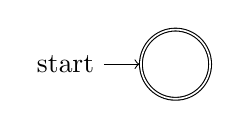
\begin{tikzpicture}
\node[initial,state,accepting] (s) {};
\end{tikzpicture}
\end{center}
หากเขียนเป็นรูปนัย จะได้ว่า $Q=\set{q_1}$, $F=\set{q_1}$, $q_1$ เป็น start state, และ $\delta(r,b)=\emptyset$ สำหรับ $r$ และ $b$ ใดๆ

\item $R=\emptyset$: จะได้ว่า $L(R)=\emptyset$ \enskip NFA ต่อไปนี้รับรู้ $L(R)$
\begin{center}
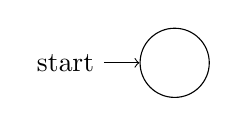
\begin{tikzpicture}
\node[initial,state] (s) {};
\end{tikzpicture}
\end{center}
หากเขียนเป็นรูปนัย จะได้ว่า $Q=\set{q_1}$, $F=\emptyset$, $q_1$ เป็น start state, และ $\delta(r,b)=\emptyset$ สำหรับ $r$ และ $b$ ใดๆ

\item $R=R_1\cup R_2$: เนื่องจาก $R_1$ เป็น regular expression ย่อยของ $R$ จะได้ว่ามี NFA $N_1$ ที่รับรู้ $L(R_1)$ เช่นเดียวกับที่มี NFA $N_2$ ที่รับรู้ $L(R_2)$ \enskip จาก Theorem~\ref{thm:dfa-union-closed-nfa} จะได้ว่าเราสามารถสร้าง NFA ที่รับรู้ $L(R_1\cup R_2)=L(R_1)\cup L(R_2)$ ได้

\item $R=R_1\circ R_2$: เช่นเดียวกับในกรณีที่แล้ว จาก Theorem~\ref{thm:dfa-concat-closed} เราสามารถสร้าง NFA ที่รับรู้ $L(R_1\circ R_2)=L(R_1)\circ L(R_2)$ ได้

\item $R=R_1^*$: เนื่องจาก $R_1$ เป็น regular expression ย่อยของ $R$ จะได้ว่ามี NFA $N_1$ ที่รับรู้ $L(R_1)$ \enskip จาก Theorem~\ref{thm:dfa-star-closed} จะได้ว่าเราสามารถสร้าง NFA ที่รับรู้ $L(R_1^*)=L(R_1)^*$ ได้
\end{enumerate}
\end{pf}
\noindent{\bf หมายเหตุ}: บทพิสูจน์โดยแยกกรณีตาม inductive definition ในลักษณะนี้ใช้\emph{การพิสูจน์โดยอุปนัยเชิงโครงสร้าง} (structural induction) โดย base cases คือกรณีฐานของ inductive definition และ inductive step คือกรณีอุปนัยของ inductive definition \enskip ใน inductive step เรามี induction hypothesis คือ $P(s)$ โดยที่ $s$ เป็นส่วนประกอบย่อยๆ ของกรณีที่เรากำลังพิสูจน์ ตัวอย่างเช่น ถ้าต้องการพิสูจน์ว่า $P(R_1\cup R_2)$ เราสามารถใช้ $P(R_1)$ และ $P(R_2)$ เป็นสมมุติฐานได้ ดังที่ได้แสดงในบทพิสูจน์ข้างต้น \enskip ในที่นี้ $P(R)$ คือ ถ้า $R$ เป็น regular expression แล้วจะมี NFA ที่รับรู้ $L(R)$
\end{lemma}
%
\begin{example}
Regular expression $(\str{a}\cup\str{b})^*\str{a}$ สามารถแปลงเป็น NFA ตามขั้นตอนวิธีข้างต้นได้ดังนี้
\begin{center}
\tikzset{initial text={},every state/.style={circle,draw,minimum size=5mm}}
\begin{longtable}{rm{3.5in}}
$\str{a}$
&
\begin{tikzpicture}
\node[initial,state] (s) {};
\node[state,accepting] (a) [right=of s] {};
\path[arrow] (s) edge node[above] {\str{a}} (a);
\end{tikzpicture}
\\
$\str{b}$
&
\begin{tikzpicture}
\node[initial,state] (s) {};
\node[state,accepting] (a) [right=of s] {};
\path[arrow] (s) edge node[above] {\str{b}} (a);
\end{tikzpicture}
\\
$\str{a}\cup\str{b}$
&
\begin{tikzpicture}
\node[initial,state] (s) {};
\node[state] (sa) [above right=5mm of s] {};
\node[state,accepting] (aa) [right=of sa] {};
\node[state] (sb) [below right=5mm of s] {};
\node[state,accepting] (ab) [right=of sb] {};

\path[arrow]
  (s) edge node[left] {$\varepsilon$} (sa)
      edge node[left] {$\varepsilon$} (sb)
  (sa) edge node[above] {\str{a}} (aa)
  (sb) edge node[above] {\str{b}} (ab);
\end{tikzpicture}
\\
$(\str{a}\cup\str{b})^*$
&
\begin{tikzpicture}
\node[initial,state,accepting] (ss) {};
\node[state] (s) [right=of ss] {};
\node[state] (sa) [above right=5mm of s] {};
\node[state,accepting] (aa) [right=of sa] {};
\node[state] (sb) [below right=5mm of s] {};
\node[state,accepting] (ab) [right=of sb] {};

\path[arrow]
  (ss) edge node[above] {$\varepsilon$} (s)
  (s) edge node[left] {$\varepsilon$} (sa)
      edge node[left] {$\varepsilon$} (sb)
  (sa) edge node[above] {\str{a}} (aa)
  (sb) edge node[above] {\str{b}} (ab)
  (aa) edge[bend right=45] node[above] {$\varepsilon$} (ss)
  (ab) edge[bend left=45] node[below] {$\varepsilon$} (ss);
\end{tikzpicture}
\\
$(\str{a}\cup\str{b})^*\str{a}$
&
\begin{tikzpicture}
\node[initial,state] (ss) {};
\node[state] (s) [right=of ss] {};
\node[state] (sa) [above right=5mm of s] {};
\node[state] (aa) [right=of sa] {};
\node[state] (sb) [below right=5mm of s] {};
\node[state] (ab) [right=of sb] {};
\node[state] (sa2) [below right=of ab] {};
\node[state,accepting] (aa2) [right=of sa2] {};

\path[arrow]
  (ss) edge node[above] {$\varepsilon$} (s)
  (s) edge node[left] {$\varepsilon$} (sa)
      edge node[left] {$\varepsilon$} (sb)
  (sa) edge node[above] {\str{a}} (aa)
  (sb) edge node[above] {\str{b}} (ab)
  (aa) edge[bend right=45] node[above] {$\varepsilon$} (ss)
  (ab) edge[bend left=45] node[below] {$\varepsilon$} (ss)
  (sa2) edge node[above] {\str{a}} (aa2)
  (aa) edge[bend left] node[right] {$\varepsilon$} (sa2)
  (ab) edge node[above] {$\varepsilon$} (sa2)
  (ss) edge[bend right=45] node[below] {$\varepsilon$} (sa2);
\end{tikzpicture}
\end{longtable}
\end{center}
อย่างไรก็ดี หากเราเข้าใจความหมายของ regular expression ตั้งต้นแล้วพยายามเขียน NFA เอง อาจจะได้ผลลัพธ์ที่เรียบง่ายกว่า ดังนี้
\begin{center}
\begin{tikzpicture}
\node[initial,state] (s) {};
\node[state,accepting] (a) [right=of s] {};
\path[arrow]
  (s) edge[loop above] node[above] {\str{a},\str{b}} (s)
      edge node[above] {\str{a}} (a);
\end{tikzpicture}
\end{center}
NFA ทั้งสองตัวนี้รับรู้ภาษาเดียวกัน กล่าวคือ หาก $\Sigma=\set{\str{a},\str{b}}$ จะได้ว่า $(\str{a}\cup\str{b})^*\str{a}$ คือ strings ที่ลงท้ายด้วย \str{a}
\end{example}

\begin{lemma}\label{lemma:dfa-regexp}
ถ้า $L$ เป็น regular language แล้ว $L$ สามารถเขียนเป็น regular expression ได้

\noindent{\bf Proof idea}: ให้ $L$ เป็น regular language \enskip จะได้ว่า มี DFA $M$ ที่รับรู้ $L$ \enskip เราจะแปลง DFA ตัวนี้ให้เป็น regular expression

การแปลงดังกล่าว จะใช้อุปกรณ์อีกอย่างหนึ่งที่เรียกว่า GNFA (generalized NFA) ซึ่งมี transitions แตกต่างไปจาก NFA ปกติ \enskip ใน NFA นั้น แต่ละ transition จะเป็นตัวอักษรเดี่ยวๆ โดยที่การเปลี่ยน state จะเกิดขึ้นได้ถ้า input symbol ตัวต่อไปตรงกับตัวอักษรที่กำกับลูกศร หรือลูกศรที่กำลังพิจารณาอยู่นั้นเป็น $\varepsilon$-transition ดังในแผนภาพต่อไปนี้ ที่อนุญาตให้เปลี่ยน state หาก input symbol ตัวต่อไปเป็น \str{a} หรือ \str{b}
\begin{center}
\begin{tikzpicture}
\node[state] (s) {};
\node[state] (a) [right=of s] {};
\path[arrow]
  (s) edge node[above] {\str{a},\str{b}} (a);
\end{tikzpicture}
\end{center}
ส่วนใน GNFA นั้น แต่ละ transitions จะเป็น regular expression โดยที่การเปลี่ยน state จะเกิดขึ้นได้ถ้า input string ที่ยังไม่อ่านเข้ามาขึ้นต้นด้วย regular expression ที่กำกับลูกศร ดังในแผนภาพต่อไปนี้ ที่อนุญาตให้เปลี่ยน state หาก input string ที่เหลือนั้นขึ้นต้นด้วย \str{a} หรือ \str{b}
\begin{center}
\begin{tikzpicture}
\node[state] (s) {};
\node[state] (a) [right=of s] {};
\path[arrow]
  (s) edge node[above] {$\str{a}\cup\str{b}$} (a);
\end{tikzpicture}
\end{center}
\end{lemma}

ก่อนจะบรรยายขั้นตอนวิธีการแปลง DFA ให้เป็น regular expression โดยใช้ GNFA จะยกตัวอย่างการแปลง DFA ที่ง่ายๆ ก่อน
\begin{example}
ให้ DFA ตั้งต้นเป็นดังนี้
\begin{center}
\begin{tikzpicture}
\node[initial,state] (1) {1};
\node[state,accepting] (2) [below=of 1] {2};

\path[arrow]
  (1) edge[loop right] node[right] {\str{a}} (1)
      edge node[right] {\str{b}} (2)
  (2) edge[loop right] node[right] {\str{a},\str{b}} (2);
\end{tikzpicture}
\end{center}
สามารถแปลงเป็น GNFA ตั้งต้นโดยเพิ่ม start และ accept states ใหม่เข้าไป จากนั้นโยง $\varepsilon$-transitions ไปหา start state เดิม และโยงจาก accept state(s) เดิม ได้ผลลัพธ์ดังนี้
\begin{center}
\begin{tikzpicture}
\node[initial,state] (s) {$s$};
\node[state] (1) [right=of s] {1};
\node[state] (2) [below=of 1] {2};
\node[state,accepting] (a) [below=of s] {$a$};

\path[arrow]
  (s) edge node[above] {$\varepsilon$} (1)
  (1) edge[loop right] node[right] {\str{a}} (1)
      edge node[right] {\str{b}} (2)
  (2) edge[loop right] node[right] {$\str{a}\cup\str{b}$} (2)
      edge node[below] {$\varepsilon$} (a);
\end{tikzpicture}
\end{center}
ลำดับถัดไป จะทำการลบ state $1$ ออก โดยปรับเปลี่ยน transitions ของ GNFA ให้ยังคงรับรู้ภาษาเดิม \enskip ทั้งนี้ หากจะลบ state ออก เส้นทางที่ GNFA เดิมเคยใช้อ่าน regular expressions โดยผ่าน state นี้ก็จะต้องทำได้เช่นเดิมใน GNFA ที่ลบ state ออกแล้ว \enskip จากแผนภาพข้างต้น จะเห็นว่า เส้นทางที่ผ่าน state $1$ นั้นมาจาก $s$ แล้วไป $2$ โดยที่อาจจะวนซ้ำที่ $1$ กี่ครั้งก็ได้ กล่าวคือ หากจะไป $2$ จาก $s$ จะต้องอ่าน input string ที่ขึ้นต้นด้วย regular expression $\varepsilon\str{a}^*\str{b}$ \enskip ดังนั้น หากจะลบ state $1$ ออก ต้องสร้าง transition โดยตรงจาก $s$ ไป $2$ ที่อ่าน $\varepsilon\str{a}^*\str{b}=\str{a}^*\str{b}$ ทำให้ได้ผลลัพธ์ดังนี้
\begin{center}
\begin{tikzpicture}
\node[initial,state] (s) {$s$};
\node[state,accepting] (a) [below=of s] {$a$};
\node[state] (2) [right=of a] {2};

\path[arrow]
  (s) edge node[right] {$\str{a}^*\str{b}$} (2)
  (2) edge[loop right] node[right] {$\str{a}\cup\str{b}$} (2)
      edge node[below] {$\varepsilon$} (a);
\end{tikzpicture}
\end{center}
ต่อไป จะทำการลบ state $2$ ออก โดยใช้หลักการเดียวกันกับการลบ state $1$ ออก \enskip จะได้ว่า เส้นทางที่ผ่าน state $2$ นั้นมาจาก $s$ แล้วไป $a$ \enskip ดังนั้น หากจะลบ state $2$ ออก ต้องสร้าง transition โดยตรงจาก $s$ ไป $a$ ที่อ่าน $\str{a}^*\str{b}(\str{a}\cup\str{b})^*$ ทำให้ได้ผลลัพธ์ดังนี้
\begin{center}
\begin{tikzpicture}
\node[initial,state] (s) {$s$};
\node[state,accepting] (a) [below=of s] {$a$};

\path[arrow]
  (s) edge node[right] {$\str{a}^*\str{b}(\str{a}\cup\str{b})^*$} (a);
\end{tikzpicture}
\end{center}
ณ ขณะนี้ GNFA ที่เรามีอยู่นั้นเหลือแค่ 2 states แล้ว จึงมีแค่ transition เดียวจาก start state ไป accept state \enskip Regular expression ที่กำกับ transition นี้คือผลลัพธ์ที่เราต้องการ

หากพิจารณาให้ถี่ถ้วน DFA ตั้งต้นนั้นตอบรับ strings ที่มี $b$ อย่างน้อยหนึ่งตัว และ regular expression ที่ได้จากการแปลงข้างต้นก็สามารถตีความได้อย่างเดียวกัน
\end{example}

ขั้นตอนการแปลง DFA ใดๆ ให้เป็น regular expression มีดังนี้
\begin{itemize}
\item จาก DFA ตั้งต้น แปลงเป็น GNFA ก่อน โดยการเพิ่ม start state ตัวใหม่ที่มี $\varepsilon$-transition ไปยัง start state เดิม และกำหนด accept state ใหม่เพียง state เดียว ที่มี $\varepsilon$-transitions มาจาก accept states เดิม \enskip ผลลัพธ์ที่ได้จะเป็น GNFA ตั้งต้น ให้ชื่อว่า $G$
\item เรียก $\textsc{convert}(G)$ ซึ่งเป็น recursive function ดังที่จะนิยามต่อไปนี้
\end{itemize}
$\textsc{convert}(G)$:
\begin{itemize}
\item ถ้า $G$ มี 2 states ให้จบการทำงาน โดยที่ 2 states นี้คือ start และ accept states \enskip Regular expression ผลลัพธ์ที่ได้ คือ regular expression ที่กำกับ transition ระหว่าง 2 states นี้

\item มิฉะนั้น เลือก state มาหนึ่ง state ที่ไม่ใช่ start และ accept states ให้ชื่อว่า $q_\mathup{rip}$ ซึ่งจะเป็น state ที่เราจะลบออกจาก GNFA \enskip จากนั้น พิจารณาคู่อันดับ $(q_i,q_j)$ ทั้งหมดที่มี transitions ผ่าน $q_\mathup{rip}$ ดังรูป
\begin{center}
\begin{tikzpicture}
\node[state] (qi) {$q_i$};
\node[state] (rip) [right=of s] {$q_\mathup{rip}$};
\node[state] (qj) [right=of rip] {$q_j$};

\path[arrow]
  (qi) edge node[above] {$R_1$} (rip)
       edge[bend right=75,distance=2.5cm] node[below] {$R_4$} (qj)
  (rip) edge[loop below] node[below] {$R_2$} (rip)
  (rip) edge node[above] {$R_3$} (qj);
\end{tikzpicture}
\end{center}
ทั้งนี้ $q_i$ และ $q_j$ ทั้งคู่ต้องไม่ใช่ $q_\mathup{rip}$ แต่ $q_i$ อาจจะเป็น state เดียวกันกับ $q_j$ ได้

หากเราจะลบ $q_\mathup{rip}$ ออกจาก GNFA เราต้องปรับเปลี่ยน transitions ของ $G$ ที่เรากำลังพิจารณาอยู่นี้ให้ยังคงรับรู้ภาษาเดิม ดังนั้น เราต้องพิจารณา states ต้นทางและปลายทางที่สามารถเดินทางผ่าน $q_\mathup{rip}$ ได้ ซึ่งก็คือคู่อันดับ $(q_i,q_j)$ ที่เป็นไปได้ทั้งหมดตามเงื่อนไขข้างต้น

\item สร้าง GNFA ใหม่ที่ชื่อว่า $G'$ โดยลบ $q_\mathup{rip}$ ออก และเปลี่ยน transition จาก $q_i$ ไป $q_j$ ในแต่ละชุดข้างต้นให้เป็นดังรูป
\begin{center}
\begin{tikzpicture}
\node[state] (qi) {$q_i$};
\node[state] (qj) [right=3cm of qi] {$q_j$};

\path[arrow]
  (qi) edge node[above] {$R_1R_2^*R_3\cup R_4$} (qj);
\end{tikzpicture}
\end{center}
นั่นคือ เมื่อลบ $q_\mathup{rip}$ ออกแล้ว เราต้องชดเชยเส้นทางที่สูญเสียไป ซึ่งก็คือจาก $q_i$ ไป $q_\mathup{rip}$ ก่อน ($R_1$) จากนั้นจะวนที่ $q_\mathup{rip}$ กี่รอบก็ได้ ($R_2^*$) และสุดท้ายออกจาก $q_\mathup{rip}$ ไปยัง $q_j$ ($R_3$) รวมทั้งหมดเป็น $R_1R_2^*R_3$ \enskip อย่างไรก็ดี อาจจะมีเส้นทางจาก $q_i$ ไป $q_j$ ที่สามารถไปได้โดยตรงโดยไม่ผ่าน $q_\mathup{rip}$ อยู่แล้ว ซึ่งเราก็ยังต้องสงวนไว้ \enskip ดังนั้น เส้นทางทั้งหมดจาก $q_i$ ไป $q_j$ ที่เป็นไปได้ ไม่ว่าจะผ่าน $q_\mathup{rip}$ หรือไม่ก็ตาม คือ $R_1R_2^*R_3\cup R_4$

\item เรียก $\textsc{convert}(G')$
\end{itemize}

\begin{example}
ในตัวอย่างนี้ จะทำการแปลง DFA ต่อไปนี้ให้เป็น regular expression
\begin{center}
\begin{tikzpicture}
\node (o) {};
\node[initial,state] (1) at ($(o)+(-2,1.5)$) {$1$};
\node[state,accepting] (2) at ($(o)+(2,1.5)$) {$2$};
\node[state,accepting] (3) at ($(o)+(0,-1.5)$) {$3$};

\path[arrow]
 (1) edge[bend left=20] node[above] {\str{a}} (2)
     edge[bend left=20] node[left] {\str{b}} (3)
 (2) edge[bend left=20] node[above] {\str{a}} (1)
     edge[loop above] node[above] {\str{b}} (2)
 (3) edge node[right] {\str{a}} (2)
     edge[bend left=20] node[left] {\str{b}} (1);
\end{tikzpicture}
\end{center}
ก่อนอื่น แปลง DFA ดังกล่าวให้เป็น GNFA ซึ่งได้ผลลัพธ์ดังนี้
\begin{center}
\begin{tikzpicture}
\node (o) {};
\node[initial,state] (s) at ($(o)+(-4,1.5)$) {$s$};
\node[state] (1) at ($(o)+(-2,1.5)$) {$1$};
\node[state] (2) at ($(o)+(2,1.5)$) {$2$};
\node[state] (3) at ($(o)+(0,-1.5)$) {$3$};
\node[state,accepting] (a) at ($(o)+(4,-1.5)$) {$a$};

\path[arrow]
 (s) edge node[above] {$\varepsilon$} (1)
 (1) edge[bend left=20] node[above] {\str{a}} (2)
     edge[bend left=20] node[left] {\str{b}} (3)
 (2) edge[bend left=20] node[above] {\str{a}} (1)
     edge[loop above] node[above] {\str{b}} (2)
     edge node[right] {$\varepsilon$} (a)
 (3) edge node[right] {\str{a}} (2)
     edge[bend left=20] node[left] {\str{b}} (1)
     edge node[above] {$\varepsilon$} (a);
\end{tikzpicture}
\end{center}
จากนั้น ทำการลบ state $1$ ออก \enskip เราต้องพิจารณาว่ามีเส้นทางใดที่ผ่าน $1$ บ้าง และหากจะลบ $1$ จะต้องชดเชยด้วย regular expression อะไร \enskip สามารถสรุปได้ดังตารางนี้
\[
\begin{array}{c|c||l}
q_i & q_j & \textup{ชดเชยด้วย} \\ \hline
s & 2 & \varepsilon\str{a} = \str{a} \\
s & 3 & \varepsilon\str{b} = \str{b} \\
2 & 2 & \str{aa}\cup\str{b} \\
2 & 3 & \str{ab} \\
3 & 2 & \str{ba}\cup\str{a} \\
3 & 3 & \str{bb}
\end{array}
\]
โปรดสังเกตว่า ในกรณี $(q_i,q_j)=(2,2)$ นั้นมี transition จาก $2$ ไป $2$ โดยตรงอยู่ก่อนแล้ว ดังนั้น ต้องไม่ลืมเส้นทางนี้ตอนเขียน regular expression ที่จะใช้ชดเชยด้วย \enskip ในกรณี $(q_i,q_j)=(3,2)$ ก็เช่นเดียวกัน

เมื่อลบ state $1$ ออก และเปลี่ยน transitions ตามตารางข้างต้นแล้ว จะได้ GNFA ใหม่ที่มีจำนวน states ลดลงไป ดังนี้
\begin{center}
\begin{tikzpicture}
\node (o) {};
\node[initial,state] (s) at ($(o)+(-4,1.5)$) {$s$};
\node[state] (2) at ($(o)+(2,1.5)$) {$2$};
\node[state] (3) at ($(o)+(0,-1.5)$) {$3$};
\node[state,accepting] (a) at ($(o)+(4,-1.5)$) {$a$};

\path[arrow]
 (s) edge node[above] {$\str{a}$} (2)
     edge node[above] {$\str{b}$} (3)
 (2) edge[loop above] node[above] {$\str{aa}\cup\str{b}$} (2)
     edge[bend right=20] node[left] {$\str{ab}$} (3)
     edge node[right] {$\varepsilon$} (a)
 (3) edge[bend right=20] node[right] {$\str{ba}\cup\str{a}$} (2)
     edge[loop below] node[below] {$\str{bb}$} (3)
     edge node[above] {$\varepsilon$} (a);
\end{tikzpicture}
\end{center}
ลำดับต่อไป จะทำการลบ state $2$ ออก \enskip เส้นทางที่ผ่าน $2$ ที่เราต้องชดเชย เป็นดังตารางนี้
\[
\begin{array}{c|c||l} % (\str{aa}\cup\str{b})^*
q_i & q_j & \textup{ชดเชยด้วย} \\ \hline
s & 3 & \str{a}(\str{aa}\cup\str{b})^*\str{ab} \cup \str{b} \\
s & a & \str{a}(\str{aa}\cup\str{b})^*\varepsilon = \str{a}(\str{aa}\cup\str{b})^* \\
3 & 3 & (\str{ba}\cup\str{a})(\str{aa}\cup\str{b})^*\str{ab} \cup \str{bb} \\
3 & a & (\str{ba}\cup\str{a})(\str{aa}\cup\str{b})^*\varepsilon \cup \varepsilon = (\str{ba}\cup\str{a})(\str{aa}\cup\str{b})^* \cup \varepsilon
\end{array}
\]
ทั้งนี้ อย่าลืม transitions โดยตรงจาก $s$ ไป $3$, จาก $3$ ไป $3$ และจาก $3$ ไป $a$ ที่มีอยู่เดิม \enskip นอกจากนี้ โปรดสังเกตด้วยว่า เราละ $\varepsilon$ ที่นำไป union ในกรณี $3$--$a$ ไม่ได้ เนื่องจาก GNFA อาจจะเปลี่ยน state จาก $3$ ไป $a$ ได้ทันทีโดยไม่ต้องอ่าน input เพิ่มเติม

GNFA ตัวถัดไปที่ยังทำงานเหมือนเดิม เป็นดังรูป
\begin{center}
\begin{tikzpicture}
\node (o) {};
\node[initial,state] (s) at ($(o)+(-4,1.5)$) {$s$};
\node[state] (3) at ($(o)+(0,-1.5)$) {$3$};
\node[state,accepting] (a) at ($(o)+(6,-1.5)$) {$a$};

\path[arrow]
 (s) edge[bend left=5] node[above right] {$\str{a}(\str{aa}\cup\str{b})^*$} (a)
     edge node[left] {$\str{a}(\str{aa}\cup\str{b})^*\str{ab}\cup\str{b}$} (3)
 (3) edge[loop below] node[below] {$(\str{ba}\cup\str{a})(\str{aa}\cup\str{b})^*\str{ab}\cup\str{bb}$} (3)
     edge node[above] {$(\str{ba}\cup\str{a})(\str{aa}\cup\str{b})^*\cup\varepsilon$} (a);
\end{tikzpicture}
\end{center}
สุดท้ายนี้ จะทำการลบ state $3$ ออก \enskip เส้นทางที่ผ่าน $3$ ที่ต้องชดเชยมีเพียงเส้นทางเดียว คือ $s$--$a$ ทำให้ได้ GNFA สุดท้ายดังนี้
\begin{center}
\begin{tikzpicture}
\node[initial,state] (s) {$s$};
\node[state,accepting] (a) [right=12cm of s] {$a$};

\path[arrow]
 (s) edge node[above] {\footnotesize $(\str{a}(\str{aa}\cup\str{b})^*\str{ab}\cup\str{b})((\str{ba}\cup\str{a})(\str{aa}\cup\str{b})^*\str{ab}\cup\str{bb})^*((\str{ba}\cup\str{a})(\str{aa}\cup\str{b})^*\cup\varepsilon)\cup\str{a}(\str{aa}\cup\str{b})^*$} (a);
\end{tikzpicture}
\end{center}
Regular expression ที่กำกับบน transition นี้เป็นผลลัพธ์จากการแปลงที่เราต้องการ
\end{example}

\begin{theorem}
$L$ is a regular language iff $L$ can be written as a regular expression.
\begin{pf}
จาก Lemmas~\ref{lemma:regexp-dfa} และ~\ref{lemma:dfa-regexp}
\end{pf}
\end{theorem}

\section{Nonregular languages}

State machines ที่เราได้เรียนรู้มาแล้วนั้นสามารถจำแนกได้เป็นสองประเภทใหญ่ๆ คือ
\begin{itemize}
\item finite state machines ซึ่งรวมถึง finite automata ที่มีจำนวนสถานะจำกัด กล่าวคือ สามารถเขียนแจกแจงเซตของ states ให้ครบทุกตัวได้ \enskip DFAs และ NFAs จัดอยู่ในกรณีนี้
\item state machines with infinite number of states ซึ่งไม่สามารถเขียนแจกแจงเซตของ states ให้ครบได้ ตัวอย่างเช่น state machine ที่จำลองการเดินของหุ่นยนต์ที่เดินทแยงได้เท่านั้น \enskip ในตัวอย่างนี้ states เป็นพิกัดจำนวนเต็มในระนาบสองมิติ ซึ่งมีจำนวนไม่จำกัด
\end{itemize}
หากพิจารณาในกรณีของ finite automata เท่านั้น ก่อนหน้านี้ เราทราบแล้วว่า ถ้า $L$ เป็น regular language แล้วเราสามารถเขียน DFA ที่รับรู้ $L$ ได้ \enskip เนื่องจาก DFA นั้นมีจำนวนสถานะที่จำกัด กล่าวคือ มีหน่วยความจำจำนวนจำกัด จะได้ว่า contrapositive ของประพจน์ดังกล่าวคือ ถ้าเราจำเป็นต้องใช้หน่วยความจำไม่จำกัดในการสร้างกลไกที่จะรับรู้ $L$ นั่นคือ ไม่มี DFA ใดๆ ที่รับรู้ $L$ ได้เลย แล้ว $L$ จะต้องไม่ใช่ regular language \enskip ภาษาที่เข้าข่ายลักษณะนี้เรียกว่า\emph{ภาษาอปรกติ} (nonregular language)s

\begin{example}
ให้ $B=\set{\str{0}^n\str{1}^n\mid n\geq 0}$ กล่าวคือ $s\in B$ ถ้า $s$ ขึ้นต้นด้วย \str{0} $n$ ตัว แล้วตามด้วย \str{1} $n$ ตัว \enskip หากเราจะพยายามสร้าง DFA ที่รับรู้ $B$ เราต้องจดจำและติดตามว่าเราได้อ่าน \str{0} เข้ามาแล้วทั้งหมดกี่ตัว เพื่อที่เราจะได้ตรวจสอบในภายหลังได้ว่า จำนวนของ \str{1} ที่ตามมานั้นมีเท่ากัน \enskip แต่ input strings ที่เป็นไปได้นั้นอาจจะยาวเท่าใดก็ได้ หาก DFA ต้องมีหน่วยความจำที่จำกัด ก็น่าจะนับจำนวน \str{0} ที่มีจำกัดได้เท่านั้น \enskip จึงดูเหมือนว่าจะเป็นไปไม่ได้ที่จะมี DFA ที่รับรู้ $B$ ได้ กล่าวคือ ดูเหมือนว่า $B$ น่าจะเป็น nonregular language
\end{example}

\begin{example}
$C=\set{w\mid\textup{$w$ มีจำนวน \str{0} และ \str{1} เท่ากัน}}$ \enskip เช่น $\str{10110010},\str{0}^n\str{1}^n,\str{1}^n\str{0}^n$ \enskip ในตัวอย่างนี้ ดูเหมือนว่าเราต้องนับจำนวน \str{0} และ \str{1} อีกเช่นกัน \enskip ดังนั้น $C$ น่าจะเป็น nonregular language ด้วย
\end{example}

\begin{example}
$D=\set{w\mid\textup{$w$ มีจำนวน \str{01} และ \str{10} ที่เป็น substrings เท่ากัน}}$ \enskip เช่น $\str{101}\in D$ เนื่องจากมี $\str{01}$ และ $\str{10}$ ปรากฏอยู่อย่างละหนึ่งครั้ง แต่ $\str{1010}\notin D$ เนื่องจากมี \str{01} ปรากฏเพียงครั้งเดียว แต่ \str{01} ปรากฏอยู่สองครั้ง \enskip ในตัวอย่างนี้ ดูเหมือนว่าเราต้องนับจำนวน \str{01} และ \str{10} เพื่อเปรียบเทียบว่าเท่ากันหรือไม่ \enskip ดังนั้น $D$ ดูแล้วน่าจะเป็น nonregular language อีกเช่นกัน
\end{example}

แท้ที่จริงแล้ว $B$ และ $C$ เป็น nonregular languages ตามที่เราคาดไว้ แต่ $D$ นั้น regular! กล่าวคือ มี DFA ที่รับรู้ $D$ \enskip แสดงว่า การคิดคำนึงแบบคร่าวๆ โดยใช้อัชฌัตติกญาณ (intuition) นั้นอาจจะทำให้เกิดข้อผิดพลาดได้ \enskip ดังนั้น หากต้องการทราบอย่างแน่ชัดว่าภาษาใดเป็น nonregular language หรือไม่ เราต้องเขียนบทพิสูจน์ที่แสดงว่าเป็นไปไม่ได้ที่จะมี DFA ที่รับรู้ภาษาที่เรากำลังพิจารณา \enskip บทพิสูจน์ในลักษณะนี้จะใช้ pumping lemma ดังที่จะได้กล่าวต่อไป

\subsection{Pumping lemma for regular languages}

Pumping lemma สำหรับ regular languages นั้นกล่าวโดยคร่าวๆ ได้ว่า regular language ทุกภาษาจะมีคุณสมบัติพิเศษ คือ ถ้า $L$ เป็น regular language และ $s\in L$ โดยที่ $s$ นั้นยาวพอ (ในที่นี้ จะต้องยาวอย่างน้อย ``pumping length'') แล้วจะมีส่วนหนึ่งของ $s$ ที่เขียนซ้ำกี่รอบก็ได้ แต่ผลลัพธ์ที่ได้ก็ยังเป็นสมาชิกของ $L$ เช่นเดิม

ดังนั้น หากจะพิสูจน์ว่า $L$ ไม่ใช่ regular language เราต้องพิสูจน์ว่า $L$ ไม่มี pumping length ที่ทำให้ $s\in L$ ใดๆ ที่ยาวอย่างน้อย pumping length มีส่วนหนึ่งสามารถเขียนซ้ำกี่รอบก็ได้และผลลัพธ์ยังคงอยู่ใน $L$

\begin{theorem}[pumping lemma]
ถ้า $A$ เป็น regular language แล้วจะมีจำนวนเต็มบวก $p$ (เรียกว่า \emph{the pumping length}) ที่ทำให้สายอักขระ $s\in A$ ใดๆ ที่มีความยาวอย่างน้อย $p$ สามารถแบ่งเป็นสามส่วน $s=xyz$ ซึ่งมีคุณสมบัติครบทุกข้อต่อไปนี้
\begin{enumerate}
\item $\forall i\geq 0: xy^iz\in A$ \label{pumping:pumped} \\
กล่าวคือ ส่วนของ $y$ จะเขียนซ้ำ (pump) กี่ครั้งก็ได้ แต่ผลลัพธ์ที่ได้ยังคงอยู่ใน $A$
\item $|y|>0$ \label{pumping:middle} \\
กล่าวคือ ความยาวของ $y$ จะต้องไม่เป็นศูนย์ นั่นคือ $y$ จะต้องไม่เป็น $\varepsilon$
\item $|xy|\leq p$ \label{pumping:short} \\
กล่าวคือ ส่วนของ $xy$ ต่อกัน ต้องมีความยาวไม่เกิน the pumping length
\end{enumerate}
\begin{pf}
ให้ $A$ เป็น regular language จะได้ว่า มี DFA $M$ ที่รับรู้ $A$ \enskip เนื่องจาก pumping lemma บังคับให้เราหาค่า $p$ สำหรับ $A$ นี้ จึงกำหนด $p$ ให้เป็นจำนวนของ states ใน $M$ \enskip ค่าของ $p$ ที่ว่านี้คือ pumping length ที่เราจะใช้ในการพิสูจน์เงื่อนไขที่เหลือ กล่าวคือ หาก $s\in A$ ยาวอย่างน้อย $p$ แล้วจะมีวิธีแบ่งส่วน $s$ ให้ตรงตามเงื่อนไขทั้งสามข้อข้างต้นได้

ให้ $s\in A$ โดยที่ $|s|\geq p$ \enskip ให้ $n$ เป็นความยาวของ $s$ กล่าวคือ $n\triangleq |s|$ และ $s=s_1s_2\ldots s_n$ โดยที่ $s_i$ เป็นตัวอักษรแต่ละตัว \enskip พิจารณาลำดับของ states ที่ $M$ ต้องใช้ในการประมวลผล $s$ ยกตัวอย่างเช่น
\[
\underbrace{q_1\xrightarrow{s_1} q_2\xrightarrow{s_2} q_5\xrightarrow{s_3} q_8 \stackrel{\cdots}{\cdots} q_{17}\xrightarrow{s_{p-1}} q_5\xrightarrow{s_p} q_9}_{\textup{$p+1$ states}}\xrightarrow{s_{p+1}} q_{13} \stackrel{\cdots}{\cdots} q_7\xrightarrow{s_n} q_6
\]
โปรดสังเกตว่า $q_1$ ต้องเป็น start state และ $q_6$ ต้องเป็น accept state เนื่องจาก $s\in A$ และ $M$ ต้อง accept $s$

จะได้ว่า หาก $M$ ต้องอ่านตัวอักษร $p$ ตัว แล้ว $M$ จะต้องมีลำดับของ states ยาว $p+1$ ตัว ที่ $M$ จะต้องใช้ในการประมวลผลตัวอักษรทั้งหมดดังกล่าว \enskip เนื่องจาก $M$ มีเพียง $p$ states แต่ต้องใช้ $p+1$ states แสดงว่าจะต้องมี state ที่ $M$ จะต้องใช้ซ้ำ \enskip ในตัวอย่างข้างต้น state ที่ใช้ซ้ำคือ $q_5$ \enskip การทำงานของ $M$ ที่ประมวลผล $s$ สามารถเขียนจำลองเป็นแผนภาพได้ดังนี้
\begin{center}
\begin{tikzpicture}
\node[initial,state] (q1) {$q_1$};
\node[state] (q5) at ($(q1)+(2,2)$) {$q_5$};
\node[state,accepting] (q6) at ($(q1)+(5,1)$) {$q_6$};

\draw[arrow,dashed]
  (q1) .. controls ($(q1)+(0,2)$) and  ($(q1)+(0.5,2)$) .. node[above] {$x$}
    ($(q1)+(0.5,1.5)$) .. controls ($(q1)+(0.5,1)$) and ($(q1)+(1,1)$) ..
    ($(q1)+(1,0)$) .. controls ($(q1)+(1,-1)$) and  ($(q1)+(1.5,0)$) ..
    ($(q1)+(1,1)$) .. controls ($(q1)+(1,2)$) and  ($(q1)+(1.5,2)$) ..
    (q5);
\draw[arrow,dashed]
  (q5) .. controls ($(q5)+(-1,0.5)$) ..
    ($(q5)+(-1,1)$) .. controls ($(q5)+(-1,2)$) and ($(q5)+(-0.5,2)$) ..
    ($(q5)+(-0.5,1)$) .. controls ($(q5)+(-0.5,0.5)$) and ($(q5)+(0,0.5)$) ..
    ($(q5)+(0,1)$) .. controls ($(q5)+(0,2)$) ..
    ($(q5)+(0.25,2)$) node[above] {$y$} .. controls ($(q5)+(0.5,2)$) ..
    ($(q5)+(0.5,1.5)$) .. controls ($(q5)+(0.5,1)$) and ($(q5)+(1,1)$) ..
    ($(q5)+(1,1.5)$) .. controls ($(q5)+(1,2)$) and ($(q5)+(1.5,2)$) ..
    ($(q5)+(1.5,1)$) .. controls ($(q5)+(1.5,0.5)$) ..
    (q5);
\draw[arrow,dashed]
  (q5) .. controls ($(q1)+(3,2)$) ..
    ($(q1)+(2.5,1)$) .. controls ($(q1)+(2.5,0)$) and ($(q1)+(3,0)$) ..
    ($(q1)+(3,1)$) .. controls ($(q1)+(3,2)$) and ($(q1)+(3.5,2)$) ..
    ($(q1)+(3.5,1)$) .. controls ($(q1)+(3.5,0)$) and ($(q1)+(4,0)$) .. node[below] {$z$}
    ($(q1)+(4,1)$) .. controls ($(q1)+(4,2)$) and ($(q1)+(4.5,2)$) ..
    (q6);
\end{tikzpicture}
\end{center}
กล่าวคือ เริ่มจาก start state, $M$ จะต้องเดินทางไปยัง state ที่ใช้ซ้ำ \enskip จากนั้น เนื่องจาก $M$ ต้องใช้ state นี้ซ้ำ จะได้ว่า ต้องมีเส้นทางที่วกกลับมาที่ state เดิมนี้ \enskip ในท้ายที่สุด $M$ ต้องเดินทางจาก state ที่ใช้ซ้ำนี้ไปยัง accept state เพื่อจบการทำงาน

เมื่อเราทราบ state ที่ใช้ซ้ำแล้ว เราสามารถแบ่ง $s$ ได้ดังนี้
\begin{itemize}
\item $x$ เป็น string ที่ $M$ ต้องอ่านตั้งแต่ต้น และพา $M$ ไปถึง state ที่ใช้ซ้ำเป็นครั้งแรก
\item $y$ เป็น string ที่ $M$ ต้องอ่านนับจาก state ที่ $M$ ใช้ซ้ำเป็นครั้งแรก และพา $M$ กลับมายัง state ที่ซ้ำนี้เป็นครั้งที่สอง
\item $z$ เป็น string ที่เหลือที่ $M$ ต้องอ่านหลังจาก $M$ กลับมายัง state ที่ต้องใช้ซ้ำเป็นครั้งที่สองแล้ว
\end{itemize}
สังเกตว่า $xyz\in A$ เนื่องจากมีลำดับของ states จาก start state ไปยัง accept state โดยวนที่ $y$ หนึ่งครั้ง \enskip นอกจากนี้ $xyyz\in A$ ด้วย โดยวนที่ $y$ สองครั้ง \enskip ในกรณีทั่วไป ไม่ว่าจะวนที่ $y$ กี่ครั้ง $xy^iz$ ก็ยังคงเป็นสมาชิกของ $A$ เช่นเดิม \enskip ยิ่งไปกว่านั้น เราสามารถเลือกที่จะไม่วนที่ $y$ เลยก็ได้ แต่ $xy^0z=xz\in A$ อยู่ดี

จากแนวคิดตามตัวอย่างข้างต้น สามารถเขียนเป็นบทพิสูจน์ในกรณีทั่วไปได้ดังต่อไปนี้

ให้ $s\in A$ โดยที่ $s=s_1s_2\ldots s_n$ และ $n\geq p$ \enskip ให้ $r_1,r_2,\ldots,r_{n+1}$ เป็นลำดับของ states ที่ $M$ ต้องใช้ในการประมวลผล $s$ \enskip จะได้ว่า $n+1\geq p+1$ (เนื่องจาก $n\geq p$) \enskip ดังนั้น ใน $p+1$ states แรกที่ $M$ ต้องใช้ จะต้องมี state $q$ ที่ $M$ ใช้ซ้ำ \enskip ให้ $r_j$ เป็นตำแหน่งแรกของ $q$ และ $r_\ell$ เป็นตำแหน่งที่สองของ $q$ ในลำดับดังกล่าว (สังเกตว่า $\ell\leq p+1$ เนื่องจาก $q$ ต้องปรากฏในลำดับอย่างน้อยสองครั้งภายใน $p+1$ ตัวแรก)

แบ่ง $s$ ออกเป็น $xyz$ โดยกำหนด $x\triangleq s_1\ldots s_{j-1}$, $y\triangleq s_j\ldots s_{\ell-1}$, และ $z\triangleq s_\ell\ldots s_n$ \enskip ต่อไป จะพิสูจน์ว่าการแบ่ง $s$ ดังกล่าวทำให้คุณสมบัติทั้งสามข้อใน pumping lemma เป็นจริง
\begin{enumerate}
\item เนื่องจาก $x$ พา $M$ จาก state $r_1$ ไปยัง state $r_j=q$, $y$ พา $M$ จาก state $r_j=q$ ไปยัง state $r_\ell=q$, และ $z$ พา $M$ จาก state $r_\ell=q$ ไปยัง state $r_{n+1}$ จะได้ว่า มีเส้นทางจาก $r_1$ ที่เป็น start state ไปยัง $r_{n+1}$ ที่เป็น accept state โดยในส่วนของ $y$ นั้นเริ่มและจบลงด้วย state เดียวกันคือ $q$ ดังนั้น ไม่ว่า $M$ จะอ่าน $y$ ทั้งหมดกี่ครั้ง (หลังจากที่อ่าน $x$ และก่อนที่จะอ่าน $z$) ก็ยังมีเส้นทางจาก $r_1$ ไป $r_{n+1}$ อยู่ดี \enskip สรุปได้ว่า $M$ ต้องตอบรับ $xy^iz$ สำหรับทุก $i\geq 0$ ด้วย
\item เนื่องจาก $y=s_j\ldots s_{\ell-1}$ มี $\ell-j$ ตัว และ $j<\ell$ ในลำดับของ states ข้างต้น จะได้ว่า $\ell-j>0$ ดังนั้น $|y|>0$
\item เนื่องจาก $xy=s_1\ldots s_{\ell-1}$ มี $\ell-1$ ตัว และ $\ell\leq p+1$ จะได้ว่า $\ell-1\leq p$ ดังนั้น $|xy|\leq p$
\end{enumerate}
ณ จุดนี้ เราได้แสดงแล้วว่าการแบ่ง $s$ ดังกล่าวทำให้ได้ส่วนต่างๆ ที่มีคุณสมบัติตามที่ต้องการ เป็นการเสร็จสิ้นบทพิสูจน์ของ pumping lemma โดยสมบูรณ์
\end{pf}
\end{theorem}

ดังนั้น หากต้องการจะพิสูจน์ว่าภาษา $B$ นั้นไม่ regular สามารถใช้ขั้นตอนต่อไปนี้ในบทพิสูจน์ได้
\begin{itemize}
\item By contradiction.  สมมุติว่า $B$ นั้น regular
\item By pumping lemma, $B$ มี pumping length $p$ ที่เราสามารถใช้ได้ในบทพิสูจน์ที่เหลือ
\item หา $s\in B$ โดยที่ $|s|\geq p$ \enskip $s$ นี้จะทำให้เกิดข้อขัดแย้งขึ้น ดังจะได้กล่าวต่อไป
\item จากนั้น ให้แสดงว่า ไม่ว่าจะแบ่ง $s=xyz$ อย่างไรก็ตาม โดยที่ $|y|>0$ (เงื่อนไขที่~\ref{pumping:middle} ใน pumping lemma เป็นจริง) และ $|xy|\leq p$ (เงื่อนไขที่~\ref{pumping:short} ใน pumping lemma เป็นจริง) แล้วจะมี $i\geq 0$ ที่ทำให้ $xy^iz\notin B$ และเกิดความขัดแย้งขึ้น
\end{itemize}
กล่าวอีกนัยหนึ่ง หากเราต้องการจะพิสูจน์ว่า $B$ ไม่ regular เราต้องแสดงว่าไม่มี pumping length ที่เป็นไปได้ \enskip ดังนั้น ไม่ว่าจะสมมุติว่า pumping length จะเป็นเท่าใดก็ตาม เราสามารถหา string $s\in B$ ที่มีความยาวอย่างน้อย pumping length นั้นๆ ที่ไม่สามารถแบ่งเป็นสามส่วนแล้วนำไป pump ได้ กล่าวคือ ไม่ว่าเราจะแบ่ง $s$ อย่างไรก็ตาม เงื่อนไขที่ตามมาทั้งสามข้อจะเป็นจริงพร้อมกันทั้งหมดไม่ได้ \enskip ในขั้นตอนข้างต้น เราให้เงื่อนไขข้อที่~\ref{pumping:middle} และ~\ref{pumping:short} เป็นจริง ดังนั้น เงื่อนไขที่~\ref{pumping:pumped} จะต้องไม่เป็นจริง \enskip หากจะแสดงว่าเงื่อนไขนี้ต้องเป็นเท็จ ก็ต้องหา $i\geq 0$ ที่ทำให้ $xy^iz\notin B$ ซึ่งทำให้เกิดความขัดแย้ง

\begin{example}\label{ex:0n1n-nonreg}
$B=\set{\str{0}^n\str{1}^n\mid n\geq 0}$ ไม่ regular

Prove by contradiction.  สมมุติว่า $B$ นั้น regular \enskip ให้ $p$ เป็น pumping length จาก pumping lemma \enskip พิจารณา $s\triangleq\str{0}^p\str{1}^p$ \enskip ไม่ว่าจะแบ่ง $s=xyz$ ด้วยวิธีใดๆ ก็ตาม โดยที่ $|xy|\leq p$ และ $|y|>0$ จะได้ว่า $xy$ ต้องประกอบไปด้วย \str{0} เท่านั้น เนื่องจาก $p$ ตัวแรกของ $s$ เป็น \str{0} ทั้งหมด \enskip ดังนั้น $y$ ต้องประกอบไปด้วย \str{0} เท่านั้นด้วย และมี \str{0} อย่างน้อย 1 ตัว เนื่องจาก $|y|$ ต้องมากกว่า 0 \enskip สมมุติว่า $y=\str{0}^k$ โดยที่ $k\geq 1$ \enskip หากพิจารณา $s'\triangleq xyyz$ จะได้ว่า $s'$ เริ่มต้นด้วย \str{0} ทั้งหมด $p+k$ ตัว ตามด้วย \str{1} ทั้งหมด $p$ ตัว กล่าวคือ $xyyz=\str{0}^{p+k}\str{1}^p$ \enskip แต่นั่นแปลว่า $xyyz\notin B$ ซึ่งขัดแย้งกับคุณสมบัติข้อที่~\ref{pumping:pumped} ใน pumping lemma $\lightning$

ดังนั้น $B$ ไม่ regular
\end{example}

\begin{example}
$C=\set{w\mid\textup{$w$ มีจำนวน \str{0} และ \str{1} เท่ากัน}}$ ไม่ regular

หากจะพิสูจน์โดยใช้ pumping lemma สามารถใช้บทพิสูจน์เดียวกันกับ Example~\ref{ex:0n1n-nonreg} ได้ ซึ่งจะทำให้ $xyyz$ มีจำนวน \str{0} และ \str{1} ไม่เท่ากัน

อย่างไรก็ดี จะแสดงการพิสูจน์อีกวิธีหนึ่ง โดยใช้สมบัติที่ว่า intersection ของ regular languages ต้องเป็น regular language กล่าวคือ regular languages มีสมบัติปิดภายใต้ intersection (Remark~\ref{rem:reg-intersect-closed})

Prove by contradiction.  สมมุติว่า $C$ นั้น regular \enskip เนื่องจาก $A\triangleq\str{0}^*\str{1}^*$ นั้น regular (เพราะเขียนเป็น regular expression ได้) จะได้ว่า $A\cap C$ ต้องเป็น regular language ด้วย \enskip แต่ \[A\cap C=\set{\str{0}^n\str{1}^n\mid n\geq 0}\] ซึ่งก็คือเซต $B$ จาก Example~\ref{ex:0n1n-nonreg} ที่เราได้พิสูจน์ไปแล้วว่าไม่ใช่ regular language $\lightning$
\end{example}

\begin{example}
$E=\set{\str{0}^i\str{1}^j\mid i>j}$ ไม่ regular

Prove by contradiction.  สมมุติว่า $E$ นั้น regular \enskip ให้ $p$ เป็น pumping length \enskip พิจารณา $s\triangleq\str{0}^{p+1}\str{1}^p$ \enskip ไม่ว่าจะแบ่ง $s=xyz$ ด้วยวิธีใดๆ ก็ตาม โดยที่ $|xy|\leq p$ และ $|y|>0$ จะได้ว่า $xy$ ต้องประกอบไปด้วย \str{0} เท่านั้น เนื่องจาก $p$ ตัวแรกของ $s$ เป็น \str{0} ทั้งหมด \enskip ดังนั้น สมมุติว่า $y=\str{0}^k$ โดยที่ $k\geq 1$ \enskip หากพิจารณา $s'\triangleq xyyz$ จะได้ว่า $s'$ เริ่มต้นด้วย \str{0} ทั้งหมด $p+1+k$ ตัว ตามด้วย \str{1} ทั้งหมด $p$ ตัว \enskip อย่างไรก็ดี ขณะนี้ยังไม่เกิดข้อขัดแย้งขึ้น เพราะ $xyyz\in E$ \enskip นอกจากนี้ $\forall i>0: xy^iz\in E$ ด้วยเหตุผลเดียวกัน

แต่ถ้า $i=0$ จะได้ว่า $xy^0z=xz$ เริ่มต้นด้วย \str{0} $p+1-k$ ตัว ตามด้วย \str{1} $p$ ตัว \enskip แต่เนื่องจาก $k\geq 1$ จะได้ว่า $p+1-k\not>p$ \enskip ดังนั้น $xz\notin E$ $\lightning$

จะเห็นว่า ในตัวอย่างนี้ เราไม่ได้ใช้ pumping lemma ในการเพิ่มจำนวนตัวอักษรเข้าไปให้เกิดข้อขัดแย้ง แต่ใช้ในการลดจำนวนตัวอักษรแทน \enskip การใช้ pumping lemma ในลักษณะนี้เรียกว่า \emph{pumping down}
\end{example}

\begin{example}\label{ex:twice-string-nonreg}
$F=\set{ww\mid w\in\set{\str{0},\str{1}}^*}$ ไม่ regular

ก่อนจะเริ่มบทพิสูจน์ ให้ทำความเข้าใจความหมายของเซตนี้ก่อน \enskip String $s\in F$ ก็ต่อเมื่อ $s$ เป็น binary string ที่สามารถแบ่งได้เป็นสองส่วน โดยที่ส่วนหน้าและส่วนหลังนั้นเหมือนกันทุกประการ เช่น $\varepsilon$ และ \str{011011}

Prove by contradiction.  สมมุติว่า $F$ นั้น regular \enskip ให้ $p$ เป็น pumping length \enskip พิจารณา $s\triangleq\str{0}^p\str{0}^p$ (สังเกตว่า $s\in F$) \enskip ณ จุดนี้ เราต้องแสดงว่า ไม่ว่าจะแบ่ง $s$ ด้วยวิธีใดๆ ก็ตาม จะทำให้ pump ส่วนตรงกลางที่แบ่งออกมาแล้วไม่ได้ทั้งหมด \enskip อย่างไรก็ดี $s$ ที่เลือกมานี้สามารถแบ่งเป็นสามส่วน $s=xyz$ ได้ โดยที่ $x\triangleq\str{0}^{p-2}$, $y\triangleq\str{00}$, และ $z\triangleq\str{0}^p$ (สังเกตว่า $|y|=2>0$ และ $|xy|=p\leq p$ ตรงตามเงื่อนไขข้อที่~\ref{pumping:middle} และ~\ref{pumping:short} ของ pumping lemma) \enskip พิจารณา $xy^iz$ \enskip ถ้า $i=0$ จะได้ว่า $xz=\str{0}^{p-2}\str{0}^p=\str{0}^{p-1}\str{0}^{p-1}\in F$ \enskip ถ้า $i=2$ จะได้ว่า $xyyz=\str{0}^{p-2}\str{0}^4\str{0}^p=\str{0}^{p+1}\str{0}^{p+1}\in F$ \enskip ในกรณีทั่วไป $xy^iz=\str{0}^{p-2}\str{0}^{2i}\str{0}^p=\str{0}^{p+i-1}\str{0}^{p+i-1}\in F$ \enskip ดังนั้น $s$ ที่เลือกมานี้ไม่ก่อให้เกิดความขัดแย้งขึ้น

ด้วยเหตุนี้ เราจึงต้องเลือก $s$ ใหม่ที่จะสร้างความขัดแย้ง \enskip พิจารณา $s'\triangleq\str{0}^p\str{1}\str{0}^p\str{1}$ \enskip ไม่ว่าจะแบ่ง $s'=xyz$ ด้วยวิธีใดๆ ก็ตาม โดยที่ $|xy|\leq p$ และ $|y|>0$ จะได้ว่า $xy$ ต้องประกอบไปด้วย \str{0} เท่านั้น เนื่องจาก $p$ ตัวแรกของ $s'$ เป็น \str{0} ทั้งหมด \enskip ดังนั้น สมมุติว่า $y=\str{0}^k$ โดยที่ $k\geq 1$ \enskip หากพิจารณา $xyyz$ จะได้ว่า $xyyz=\str{0}^{p+k}\str{1}\str{0}^p\str{1}\notin F$ $\lightning$
\end{example}

\section{Context-free grammars}

หากกล่าวถึง\emph{ไวยากรณ์} (grammar)s สิ่งแรกที่อาจจะนึกถึงคือ ไวยากรณ์ภาษาอังกฤษ ที่กำหนดวิธีการเขียนประโยคต่างๆ ให้ถูกหลักการ \enskip ตัวอย่างเช่น ลำดับของคำต่อไปนี้เป็นประโยคที่ถูกต้องตามหลักไวยากรณ์ในภาษาอังกฤษ
\[
\str{I think that you believe that he suspects that his girlfriend cheated on him}
\]
หากสังเกตประโยคข้างต้นให้ละเอียดถี่ถ้วน จะเห็นว่า ประโยคดังกล่าวมี\emph{โครงสร้างเวียนบังเกิด} (recursive structure) กล่าวคือ ส่วนท้ายของประโยค (ที่ขึ้นต้นด้วย \str{that} แต่ละตัว) ประกอบด้วยอนุประโยคที่ซ้อนกันโดยไม่จำกัดได้ \enskip ในกรณีทั่วไป ส่วนใดส่วนหนึ่งของประโยคอาจจะแทนที่ได้ด้วยจำนวนคำที่มากขึ้น โดยที่กลุ่มคำเหล่านั้นยังทำให้ถูกหลักไวยากรณ์เหมือนเดิม เช่น จากประโยค \str{I think that you are cute} เราสามารถแทนที่อนุประโยค \str{you are cute} ด้วย \str{I think that you are cute} ได้ กลายเป็น \str{I think that I think that you are cute} ซึ่งยังถูกหลักไวยากรณ์อยู่ และเราสามารถแทนที่แบบนี้ไปได้เรื่อยๆ ไม่มีที่สิ้นสุด

หากจะเขียนไวยากรณ์ภาษาอังกฤษออกมาเป็นกลุ่มของกฎ อาจจะได้ดังรายการต่อไปนี้ ซึ่งทำให้ก่อกำเนิดประโยคในภาษาอังกฤษแบบง่ายๆ ได้ (สังเกตว่า จำนวนประโยคผลลัพธ์ที่เป็นไปได้นั้นมีไม่จำกัด)
\begin{align*}
\ntl{sentence}
 &\to \ntl{noun-phrase}\ntl{verb-phrase} \\
\ntl{noun-phrase}
 &\to \ntl{noun} \\
\ntl{noun-phrase}
 &\to \ntl{adjective}\ntl{noun} \\
\ntl{verb-phrase}
 &\to \ntl{complex-verb} \\
\ntl{verb-phrase}
 &\to \ntl{complex-verb}\ntl{prep-phrase} \\
\ntl{prep-phrase}
 &\to \ntl{prep}\ntl{noun-phrase} \\
\ntl{complex-verb}
 &\to \ntl{verb} \\
\ntl{complex-verb}
 &\to \ntl{verb}\ntl{noun-phrase} \\
\ntl{noun}
 &\to \str{I}\mid\str{you}\mid\str{he}\mid\str{girlfriend}\mid\str{him} \\
\ntl{verb}
 &\to \str{think}\mid\str{believe}\mid\str{suspects}\mid\str{cheated} \\
\ntl{adjective}
 &\to \str{his} \\
\ntl{prep}
 &\to \str{on}\mid\str{that}
\end{align*}
กฎในบรรทัดแรกข้างต้นกล่าวว่า ประโยคใดๆ ประกอบด้วยสองส่วน คือ นามวลี (noun phrase) และกริยาวลี (verb phrase) \enskip กฎที่สองกล่าวว่า นามวลีอาจจะเป็นคำนาม (noun) ได้ ในขณะเดียวกัน กฎข้อที่สามกล่าวว่า นามวลีอาจจะประกอบด้วยคำคุณศัพท์ (adjective) ต่อด้วยคำตามก็ได้ กล่าวคือ นามวลีใดๆ อาจจะเป็นได้สองแบบ \enskip ในส่วนของบุพบทวลี (preposition phrase) นั้น ต้องขึ้นต้นด้วยคำบุพบท (preposition) แล้วตามด้วยนามวลี \enskip สังเกตว่า ในส่วนย่อยๆ ของประโยคนั้น อาจจะอ้างอิงส่วนของประโยคที่เคยใช้มาแล้วก่อนหน้านี้ (ในกรณีของบุพบทวลี สามารถใช้นามวลีเป็นส่วนย่อยได้)

ไวยากรณ์ที่เขียนได้ในลักษณะนี้เรียกว่า\emph{ไวยากรณ์ไม่พึ่งบริบท} (context-free grammar)s

หากต้องการพิจารณาว่าประโยค \str{his girlfriend is cheated on him} นั้นเกิดจากไวยากรณ์ที่กำหนดให้ได้หรือไม่ สามารถเขียนลำดับ\emph{การแปลง} (derivation) ได้ดังนี้
\begin{align*}
\ntl{sentence}
 &\Rightarrow \ntl{noun-phrase}\ \ntl{verb-phrase} \\
 &\Rightarrow \ntl{adjective}\ \ntl{noun}\ \ntl{verb-phrase} \\
 &\Rightarrow \str{his}\ \ntl{noun}\ \ntl{verb-phrase} \\
 &\Rightarrow \str{his}\ \str{girlfriend}\ \ntl{verb-phrase} \\
 &\Rightarrow \str{his}\ \str{girlfriend}\ \ntl{complex-verb}\ \ntl{prep-phrase} \\
 &\Rightarrow \str{his}\ \str{girlfriend}\ \ntl{verb}\ \ntl{prep-phrase} \\
 &\Rightarrow \str{his}\ \str{girlfriend}\ \str{cheated}\ \ntl{prep-phrase} \\
 &\Rightarrow \str{his}\ \str{girlfriend}\ \str{cheated}\ \ntl{prep}\ \ntl{noun-phrase} \\
 &\Rightarrow \str{his}\ \str{girlfriend}\ \str{cheated}\ \str{on}\ \ntl{noun-phrase} \\
 &\Rightarrow \str{his}\ \str{girlfriend}\ \str{cheated}\ \str{on}\ \ntl{noun} \\
 &\Rightarrow \str{his}\ \str{girlfriend}\ \str{cheated}\ \str{on}\ \str{him}
\end{align*}
ในแต่ละขั้นของลำดับการแปลงนั้น เราเลือกส่วนของประโยคที่ยังขยายต่อได้ มาขยายตามกฎใดกฎหนึ่งที่กำหนดไว้ ตัวอย่างเช่น ในการแปลงจากบรรทัดแรกไปยังบรรทัดที่สองข้างต้น เราเลือกขยายส่วนของ \ntl{noun-phrase} ออกเป็น \ntl{adjective}\ntl{noun} โดยใช้กฎข้อที่สามจากไวยากรณ์ก่อนหน้านี้ \enskip ทำเช่นนี้ไปเรื่อยๆ จนกว่าจะไม่มีตัวที่ขยายต่อได้อีก \enskip สังเกตว่า ในลำดับการแปลงข้างต้นนี้ เราเลือกที่จะแปลงสัญลักษณ์ตัวซ้ายสุดที่ยังขยายได้อยู่ การแปลงในลักษณะนี้เรียกว่า\emph{การแปลงจากตัวซ้ายสุด} (leftmost derivation) \enskip ในทางกลับกัน หากเราเลือกแปลงสัญลักษณ์ตัวขวาสุดที่ยังขยายได้อยู่ก่อนเสมอ จะเรียกว่า\emph{การแปลงจากตัวขวาสุด} (rightmost derivation) \enskip หากต้องการเขียน rightmost derivation ของประโยค \str{his girlfriend cheated on him} สามารถเขียนได้ดังนี้
\begin{align*}
\ntl{sentence}
 &\Rightarrow \ntl{noun-phrase}\ \ntl{verb-phrase} \\
 &\Rightarrow \ntl{noun-phrase}\ \ntl{complex-verb}\ \ntl{prep-phrase} \\
 &\Rightarrow \ntl{noun-phrase}\ \ntl{complex-verb}\ \ntl{prep}\ \ntl{noun-phrase} \\
 &\Rightarrow \ntl{noun-phrase}\ \ntl{complex-verb}\ \ntl{prep}\ \ntl{noun} \\
 &\Rightarrow \ntl{noun-phrase}\ \ntl{complex-verb}\ \ntl{prep}\ \str{him} \\
 &\Rightarrow \ntl{noun-phrase}\ \ntl{complex-verb}\ \str{on}\ \str{him} \\
 &\Rightarrow \ntl{noun-phrase}\ \ntl{verb}\ \str{on}\ \str{him} \\
 &\Rightarrow \ntl{noun-phrase}\ \str{cheated}\ \str{on}\ \str{him} \\
 &\Rightarrow \ntl{adjective}\ \ntl{noun}\ \str{cheated}\ \str{on}\ \str{him} \\
 &\Rightarrow \ntl{adjective}\ \str{girlfriend}\ \str{cheated}\ \str{on}\ \str{him} \\
 &\Rightarrow \str{his}\ \str{girlfriend}\ \str{cheated}\ \str{on}\ \str{him}
\end{align*}

อย่างไรก็ดี จะเห็นว่าการเขียน derivation นั้นเกิดความซ้ำซ้อนขึ้น เนื่องจากเราต้องเขียนส่วนของประโยคที่ขยายจนเสร็จสิ้นสมบูรณ์แล้วซ้ำหลายๆ ครั้ง จนกว่าการแปลงจะเสร็จสิ้นสมบูรณ์ทั้งหมด \enskip หากจะลดความซ้ำซ้อน เราสามารถเขียนการแปลงดังกล่าวในรูปของ\emph{ต้นไม้แจงส่วน} (parse tree) ได้ดังรูปที่~\ref{fig:parse-tree}
%
\begin{figure}
\begin{center}
\begin{tikzpicture}[level 1/.style={sibling distance=10em},level 2/.style={sibling distance=5em},level 3/.style={sibling distance=2.5em},level distance=3em]
\node {\textit{S}}
  child {
    node {\textit{NP}}
    child {
      node {\textit{ADJ}}
      child { node {\str{his}} }
    }
    child {
      node {\textit{N}}
      child { node {\str{girlfriend}} }
    }
  }
  child {
    node {\textit{VP}}
    child {
      node {\textit{CV}}
      child {
        node {\textit{V}}
        child { node {\str{cheated}} }
      }
    }
    child {
      node {\textit{PP}}
      child {
        node {\textit{P}}
        child { node {\str{on}} }
      }
      child {
        node {\textit{NP}}
        child {
          node {\textit{N}}
          child { node {\str{him}} }
        }
      }
    }
  }
;
\end{tikzpicture}
\end{center}
\caption{Parse tree for the sentence \str{his girlfriend cheated on him}}
\label{fig:parse-tree}
\end{figure}
%
จะเห็นว่า ส่วนต่างๆ ของประโยคนั้นสามารถเขียนเพียงครั้งเดียวใน parse tree ได้ โดยสามารถอ่านผลลัพธ์ที่ได้จากซ้ายไปขวา \enskip อย่างไรก็ดี การเขียน parse trees ก็ทำให้เราสูญเสียข้อมูลบางอย่างไปด้วย \enskip ในที่นี้ เราไม่สามารถแยกแยะได้ว่า ลำดับการแปลงตั้งแต่ต้นจนจบเป็นอย่างไร อาจจะเป็น leftmost derivation, rightmost derivation, หรือ derivations แบบอื่นก็ได้

ก่อนจะนิยาม context-free grammars เป็นรูปนัย จะขอยกตัวอย่างอีกหนึ่งตัวอย่างก่อน
\begin{example}\label{ex:cfg-0n-sharp-1n}
พิจารณา context-free grammar ต่อไปนี้
\begin{align*}
A &\to \str{0}A\str{1} \\
A &\to B \\
B &\to \str{\#}
\end{align*}
หากเริ่มแปลงจากสัญลักษณ์ $A$ ตัวอย่างของสายอักขระที่เป็นไปได้ รวมถึง parse tree และ leftmost derivation ที่ควบคู่กับสายอักขระแต่ละตัว มีดังนี้
\begin{itemize}
\begin{multicols}{3}
\item \str{0\#1}:
\begin{center}
\begin{tikzpicture}[sibling distance=2.5em,level distance=2.5em]
\node {$A$}
  child { node {\str{0}} }
  child {
    node {$B$}
    child { node {\str{\#}} }
  }
  child { node {\str{1}} }
;
\end{tikzpicture}
\end{center}
\begin{align*}
A
 &\Rightarrow \str{0}A\str{1} \\
 &\Rightarrow \str{0}B\str{1} \\
 &\Rightarrow \str{0}\str{\#}\str{1} \\
\end{align*}
\end{multicols}

\begin{multicols}{3}
\item \str{00\#11}:
\begin{center}
\begin{tikzpicture}[sibling distance=2.5em,level distance=2.5em]
\node {$A$}
  child { node {\str{0}} }
  child {
    node {$A$}
    child { node {\str{0}} }
    child {
      node {$B$}
      child { node {\str{\#}} }
    }
    child { node {\str{1}} }
  }
  child { node {\str{1}} }
;
\end{tikzpicture}
\end{center}
\begin{align*}
A
 &\Rightarrow \str{0}A\str{1} \\
 &\Rightarrow \str{0}\str{0}A\str{1}\str{1} \\
 &\Rightarrow \str{0}\str{0}B\str{1}\str{1} \\
 &\Rightarrow \str{0}\str{0}\str{\#}\str{1}\str{1} \\
\end{align*}
\end{multicols}

\begin{multicols}{3}
\item \str{\#}:
\begin{center}
\begin{tikzpicture}[sibling distance=2.5em,level distance=2.5em]
\node {$A$}
  child {
    node {$B$}
    child { node {\str{\#}} }
  }
;
\end{tikzpicture}
\end{center}
\begin{align*}
A
 &\Rightarrow B \\
 &\Rightarrow \str{\#} \\
\end{align*}
\end{multicols}
\end{itemize}

หากพิจารณาให้ถี่ถ้วน จะเห็นว่า grammar นี้\emph{ก่อกำเนิด} (generate)s ภาษา $\set{\str{0}^n\str{\#}\str{1}^n\mid n\geq 0}$ กล่าวคือ เราสามารถเริ่มด้วย \str{\#} ได้ (โดยใช้กฎ $A\to B$) จากนั้น หาก $s$ เป็น string ใดๆ ที่เรามีอยู่แล้ว เราสามารถนำ \str{0} มาปะหน้า และนำ \str{1} มาต่อท้ายไปพร้อมๆ กัน (โดยใช้กฎ $A\to\str{0}A\str{1}$) นั่นคือ จำนวน \str{0} ก่อนหน้า \str{\#} ต้องเท่ากับจำนวน \str{1} ที่อยู่หลัง \str{\#}
\end{example}

ส่วนต่างๆ ของ context-free grammar มีดังนี้
\begin{itemize}
\item สัญลักษณ์ที่เป็นตัวอักษรในสายอักขระ ซึ่งไม่สามารถขยายต่อได้อีก เช่น \str{0} เรียกว่า\emph{สัญลักษณ์ปลายทาง} (terminal symbol)
\item สัญลักษณ์ที่อยู่ในรูปตัวแปร ซึ่งสามารถขยายต่อได้อีก เช่น $A$ เรียกว่า\emph{สัญลักษณ์ระหว่างทาง} (nonterminal symbol)
\item กฎแต่ละตัวที่จะแปลงจาก nonterminal symbol ไปยังส่วนย่อยๆ เช่น $B\to\str{\#}$ เรียกว่า\emph{กฎการผลิต} (production rule)
\end{itemize}

\begin{definition}
\emph{ไวยากรณ์ไม่พึ่งบริบท} (context-free grammar) [CFG] ประกอบด้วย 4 ส่วนดังนี้
\begin{itemize}
\item $V$ เป็นเซตจำกัด (finite set) ของ nonterminal symbols
\item $\Sigma$ เป็น finite set ของ terminal symbols
\item $R$ เป็น finite set ของ production rules ซึ่งแต่ละกฎจะอยู่ในรูป $N\to(V\cup\Sigma)^*$ โดยที่ $N\in V$
\item $S\in V$ เป็น start nonterminal symbol
\end{itemize}

ภาษาที่ก่อกำเนิดได้โดย context-free grammars เรียกว่า\emph{ภาษาไม่พึ่งบริบท} (context-free language)s [CFL]s
\end{definition}
%
\begin{example}
หากเขียน CFG ใน Example~\ref{ex:cfg-0n-sharp-1n} เป็นรูปนัย จะได้ว่า
\begin{itemize}
\item $V=\set{A,B}$
\item $\Sigma=\set{\str{0},\str{1},\str{\#}}$
\item $R=\set{A\to\str{0}A\str{1},A\to B,B\to\str{\#}}$
\item $A$ เป็น start nonterminal symbol
\end{itemize}
\end{example}

ทั้งนี้ หาก nonterminal symbol ใดมี production rules ที่เป็นไปได้หลายตัว สามารถใช้เครื่องหมาย $\mid$ เขียนแยกคั่นกรณีได้ เช่น $A\to\str{0}A\str{1}\mid B$

\begin{example}
พิจารณา $B=\set{\str{0}^n\str{1}^n\mid n\geq 0}$ \enskip หากต้องการพิสูจน์ว่า $B$ เป็น CFL ต้องหา CFG ที่ก่อกำเนิด $B$ \enskip CFG ดังกล่าวสามารถเขียนได้ดังนี้
\begin{align*}
S &\to \str{0}S\str{1} \mid E \\
E &\to \varepsilon
\end{align*}
กล่าวคือ strings ใน $B$ สามารถเป็นได้สองกรณี ในกรณีหลัง เป็น empty string ($\varepsilon$) ได้ ในกรณีแรก หาก string ใดเป็นสมาชิกของ $B$ อยู่แล้ว ก็สามารถนำ \str{0} ปะหน้า และ \str{1} ต่อท้ายในเวลาเดียวกัน โดยผลลัพธ์ที่ได้จะเป็นสมาชิกของ $B$ เหมือนเดิม \enskip หากต้องการเขียน grammar ดังกล่าวโดยใช้ nonterminal symbol เพียงแค่ตัวเดียว สามารถเขียนได้ดังนี้
\[S \to \str{0}S\str{1} \mid \varepsilon\]
\end{example}

\begin{example}
ให้ $\Sigma=\set{\str{a},\str{b}}$ \enskip พิจารณา CFG ต่อไปนี้
\[S \to \str{a}S\str{b} \mid SS \mid \varepsilon\]
หากต้องการหาว่า CFG ดังกล่าวก่อกำเนิดภาษาใด เริ่มแรกอาจจะยังเห็นภาพไม่ชัดเจน ต้องลองเขียน strings บางตัวที่เกิดจาก grammar นี้ได้ก่อน เช่น \str{aaabbb}, \str{abab}, $\varepsilon$, และ \str{aababb} หากพิจารณาให้ถี่ถ้วน จะเห็นว่า strings ในภาษานี้สามารถสร้างได้ 3 วิธี กล่าวคือ
\begin{itemize}
\item หาก $s$ อยู่ในภาษานี้ เราสามารถเติม \str{a} ปะหน้า และ \str{b} ต่อท้าย ก็จะได้ผลลัพธ์ที่ยังอยู่ในภาษานี้ด้วย
\item หาก $s_1$ และ $s_2$ อยู่ในภาษานี้ เราสามารถนำ $s_1$ และ $s_2$ มาต่อกันเป็น $s_1s_2$ ซึ่งก็จะอยู่ในภาษานี้ด้วย
\item $\varepsilon$ อยู่ในภาษานี้
\end{itemize}
แม้ว่าจะพิจารณาแยกกรณีดังกล่าวข้างต้นแล้ว ภาษาที่ต้องการหาอาจจะยังไม่ชัดเจน \enskip หากเปลี่ยน \str{a} แต่ละตัวให้เป็นวงเล็บเปิด \str{(} และ \str{b} แต่ละตัวให้เป็นวงเล็บปิด \str{)} จะได้ว่าตัวอย่าง strings ข้างต้นกลายเป็น \str{((()))}, \str{()()}, $\varepsilon$, และ \str{(()())} ซึ่งสามารถตีความได้เป็น strings ของวงเล็บที่ซ้อนในได้อย่างถูกต้อง (properly nested parentheses) กล่าวคือ strings ในลักษณะนี้สามารถสร้างได้สามวิธีด้วยกัน คือ
\begin{itemize}
\item หาก $s$ เป็นวงเล็บที่ซ้อนในอยู่อย่างถูกต้อง เราสามารถเติม \str{(} ปะหน้า และ \str{)} ต่อท้าย ก็จะได้ผลลัพธ์ที่ยังซ้อนในอย่างถูกต้องเหมือนเดิม
\item หาก $s_1$ และ $s_2$ เป็นวงเล็บที่ซ้อนในอยู่อย่างถูกต้อง เราสามารถนำ $s_1$ และ $s_2$ มาต่อกันเป็น $s_1s_2$ ซึ่งวงเล็บก็ยังซ้อนในได้อย่างถูกต้องเหมือนเดิม
\item $\varepsilon$ มีวงเล็บซ้อนในได้ถูกต้อง เนื่องจากไม่มีวงเล็บเลย เงื่อนไขจึงเป็นจริงโดยปริยาย
\end{itemize}
\end{example}

\begin{example}
หากต้องการเขียน CFG ที่ก่อกำเนิดนิพจน์เลขคณิต (arithmetic expressions) โดยที่ $\Sigma=\set{\str{a},\str{+},\str{*},\str{(},\str{)}}$ สามารถเขียนได้ดังนี้
\[
\begin{array}{ccl}
E
 &\to& E\str{+}E \\
 &\mid& E\str{*}E \\
 &\mid& \str{(}E\str{)} \\
 &\mid& \str{a}
\end{array}
\]
อย่างไรก็ดี หากต้องการ parse \str{a+a*a} จะได้ผลลัพธ์ซึ่งเป็น parse trees มากกว่าหนึ่งแบบ ดังนี้
\begin{center}
\hfill
\begin{tikzpicture}[sibling distance=2.5em,level distance=2.5em]
\node {$E$}
  child {
    node {$E$}
    child { node {\str{a}} }
  }
  child { node {\str{+}} }
  child {
    node {$E$}
    child {
      node {$E$}
      child { node {\str{a}} }
    }
    child { node {\str{*}} }
    child {
      node {$E$}
      child { node {\str{a}} }
    }
  }
;
\end{tikzpicture}
%
\hfill
%
\begin{tikzpicture}[sibling distance=2.5em,level distance=2.5em]
\node {$E$}
  child {
    node {$E$}
    child {
      node {$E$}
      child { node {\str{a}} }
    }
    child { node {\str{+}} }
    child {
      node {$E$}
      child { node {\str{a}} }
    }
  }
  child { node {\str{*}} }
  child {
    node {$E$}
    child { node {\str{a}} }
  }
;
\end{tikzpicture}
\hspace*{\fill}
\end{center}
ในแบบแรก เราทำการบวกเป็นลำดับสุดท้าย เพื่อประกอบ arithmetic expressions ย่อย \str{a} และ \str{a*a} เข้าด้วยกัน \enskip ในแบบหลัง เราทำการคูณเป็นลำดับสุดท้าย เพื่อเชื่อม arithmetic expressions ย่อย \str{a+a} และ \str{a} เข้าด้วยกัน \enskip เนื่องจาก string ดังกล่าวมีหลาย parse trees จึงกล่าวว่า string \str{a+a*a} นี้\emph{แปลงมาอย่างกำกวม} (derived ambiguously) เนื่องจากลำดับการบวกและคูณนั้นไม่กำหนดแน่ชัด \enskip ดังนั้น grammar นี้มีความ\emph{กำกวม} (ambiguous) \enskip นอกจากนี้ string \str{a+a+a} ก็แปลงได้อย่างกำกวมด้วย เนื่องจากเราไม่สามารถกำหนดแน่ชัดได้ว่า จะทำการบวกตัวหน้าหรือตัวหลังก่อน

อย่างไรก็ดี ตามหลักคณิตศาสตร์แล้ว เราควรจะทำการคูณก่อนบวก และบวกตัวซ้ายก่อนตัวขวา \enskip นั่นคือ หากจะประกอบ arithmetic expression ที่ใหญ่ขึ้น ต้องประกอบโดยใช้การบวกหลังการใช้การคูณ และต้องประกอบการบวกตัวซ้ายก่อนที่จะประกอบการบวกตัวขวา ทั้งนี้ หากมีนิพจน์ที่อยู่ในวงเล็บ ต้องประกอบส่วนที่อยู่ในวงเล็บให้เสร็จสิ้นสมบูรณ์ก่อน โดยใช้หลักการเดียวกันกับที่ได้กล่าวมา

จากแนวคิดดังกล่าว เราสามารถทำ\emph{การแก้ไขความกำกวม} (disambiguation) ได้ โดยเขียน CFG ใหม่ที่ยังรับรู้ภาษาเดิม แต่ไม่ทำให้มี strings ที่เขียน parse tree หลายแบบได้ ดังนี้
\begin{align*}
\ntl{expr} &\to \ntl{expr}\str{+}\ntl{term} \mid \ntl{term} \\
\ntl{term} &\to \ntl{term}\str{*}\ntl{factor} \mid \ntl{factor} \\
\ntl{factor} &\to \str{(}\ntl{expr}\str{)} \mid \str{a}
\end{align*}
ในที่นี้ \ntl{expr} คือนิพจน์เลขคณิตทั้งหมดที่เป็นไปได้, \ntl{term} คือนิพจน์เลขคณิตที่ไม่มีเครื่องหมายบวก ยกเว้นจะอยู่ภายในวงเล็บ, และ \ntl{factor} คือนิพจน์เลขคณิตที่ไม่มีเครื่องหมายคูณ ยกเว้นจะอยู่ภายในวงเล็บ \enskip ในที่นี้ ส่วนที่อยู่ในวงเล็บจะเป็น expression อะไรก็ได้ไม่จำกัด \enskip หากใช้ grammar ดังกล่าว \str{a+a*a} จะเหลือเพียง parse tree เดียวดังนี้
\begin{center}
\begin{tikzpicture}[sibling distance=2.5em,level distance=2.5em]
\node {$E$}
  child {
    node {$E$}
    child {
      node {$T$}
      child {
        node {$F$}
        child { node {\str{a}} }
      }
    }
  }
  child { node {\str{+}} }
  child {
    node {$T$}
    child {
      node {$T$}
      child {
        node {$F$}
        child { node {\str{a}} }
      }
    }
    child { node {\str{*}} }
    child {
      node {$F$}
      child { node {\str{a}} }
    }
  }
;
\end{tikzpicture}
\end{center}
\end{example}
ในตัวอย่างข้างต้น เราสามารถเขียน CFG ใหม่ที่ไม่กำกวมได้ อย่างไรก็ดี มี context-free languages ที่ทุกๆ context-free grammar ที่ก่อกำเนิดภาษานั้นๆ ต้องกำกวม \enskip ภาษาในลักษณะนี้เรียกว่ามีความ\emph{กำกวมในตัว} (inherently ambiguous)
%
\begin{example}
$\set{\str{a}^i\str{b}^j\str{c}^k\mid i=j \vee j=k}$ is an inherently ambiguous context-free language.
\end{example}

\begin{exercise}
    เขียน context-free grammar ที่ก่อกำเนิดภาษาข้างต้น แล้วหา string ที่สามารถตีความได้สองวิธีใน grammar ดังกล่าว พร้อมทั้งเขียน parse trees ของการตึความแต่ละวิธีด้วย
\end{exercise}

\begin{example}
อีกตัวอย่างหนึ่งของความกำกวมนั้นเกิดขึ้นในภาษาโปรแกรม (programming languages) \enskip ปัญหานี้เรียกว่า \emph{dangling else} problem ซึ่งมีอยู่ว่า หากเขียนโปรแกรมที่ใช้เงื่อนไขโดยปฏิบัติไม่ครบทุกกรณีในลักษณะนี้
\begin{lstlisting}[language=haskell]
if (b1) then if (b2) then C1 else C2
\end{lstlisting}
ควรจะตีความประโยคดังกล่าวเป็นอย่างไร \enskip ในที่นี้ สามารถตีความได้สองวิธี
\begin{multicols}{2}
\begin{lstlisting}[language=haskell]
if (b1) then {
  if (b2) then
    C1
  else
    C2
}
\end{lstlisting}

\begin{lstlisting}[language=haskell]
if (b1) then {
  if (b2) then
    C1
}
else
  C2
\end{lstlisting}
\end{multicols}
ในวิธีด้านซ้าย ส่วนของ \str{else} ผูกอยู่กับ \str{if} ตัวใน ส่วนในวิธีด้านขวา ส่วนของ \str{else} ผูกอยู่กับ \str{if} ตัวนอก

ปัญหา dangling else เป็นปัญหาเก่าแก่ ที่นักออกแบบภาษาต้องเผชิญและตัดสินใจเลือกตีความประโยคดังกล่าวเป็นอย่างใดอย่างหนึ่ง \enskip ในวงการออกแบบและพัฒนาภาษาโปรแกรมคอมพิวเตอร์ เป็นที่ยอมรับโดยทั่วไปว่าการตีความแบบทางด้านซ้ายจะเหมาะสมกว่า กล่าวคือ \lstinline[language=java]{else} ควรจะคู่กับ \lstinline[language=java]{if} ตัวที่ใกล้ที่สุด หากต้องการเป็นอย่างอื่นควรระบุให้ชัดเจน (เช่น ใส่เครื่องหมายปีกกาคร่อม) \enskip ในที่นี้ เราสามารถเขียน grammar ที่เลือกตีความเป็นแบบแรกได้
\end{example}

ตัวอย่างดังกล่าวเป็นเพียงส่วนหนึ่งของภาษาโปรแกรมเท่านั้น อย่างไรก็ดี programming languages ที่ใช้กันอยู่ในปัจจุบันเกือบทั้งหมดสามารถเขียน\emph{วากยสัมพันธ์} (syntax) เป็น context-free grammars ที่ไม่กำกวมได้

\subsection{Pushdown automata}

ณ จุดนี้ เราได้กล่าวถึง context-free languages และ context-free grammars มาพอสมควร \enskip หากจะย้อนกลับไปเนื้อหาที่เกี่ยวกับ regular languages จะเห็นว่า context-free languages นั้นมีบทบาทในลักษณะเดียวกันกับ regular expressions กล่าวคือ ทั้งสองอย่างนี้ก่อกำเนิดภาษาขึ้นมา \enskip คำถามที่อาจจะตามมาคือ มีกลไกใดหรือไม่ที่รับรู้ context-free languages เช่นเดียวกับที่ finite automata รับรู้ regular languages

กลไกที่รับรู้ context-free languages เรียกว่า \emph{pushdown automata} [PDA] ซึ่งเป็นส่วนต่อขยายมาจาก NFA โดยเพิ่ม\emph{กองซ้อน} (stack) เข้าไป ทำให้สามารถใช้หน่วยความจำได้ไม่จำกัด
%
\begin{example}
PDA ที่รับรู้ $B=\set{\str{0}^n\str{1}^n\mid n\geq 0}$ สามารถเขียนเป็นแผนภาพได้ดังนี้
\begin{center}
\begin{tikzpicture}[node distance=2cm]
\node[initial,state,accepting] (q0) {$q_0$};
\node[state] (q1) [right=of q0] {$q_1$};
\node[state] (q2) [below=of q1] {$q_2$};
\node[state,accepting] (q3) [left=of q2] {$q_3$};

\path[arrow]
  (q0) edge node [above] {$\varepsilon$, $\varepsilon\to\str{\$}$} (q1)
  (q1) edge[loop right] node [right] {\str{0}, $\varepsilon\to\str{0}$} (q1)
       edge node [right] {\str{1}, $\str{0}\to\varepsilon$} (q2)
  (q2) edge[loop right] node [right] {\str{1}, $\str{0}\to\varepsilon$} (q2)
       edge node [above] {$\varepsilon$, $\str{\$}\to\varepsilon$} (q3)
;
\end{tikzpicture}
\end{center}
เริ่มแรก $q_0$ เป็น accept state เนื่องจาก $\varepsilon\in B$ \enskip หลักการของ PDA ดังกล่าวจะนับว่าจำนวน \str{0} มีเท่าจำนวน \str{1} หรือไม่ โดยหากตัวอักษรที่อ่านเข้ามาเป็น \str{0} ให้ push \str{0} ลงใน stack (transition จาก $q_1$ ไป $q_1$ โดยส่วนที่เขียนว่า $\varepsilon\to\str{0}$ หมายความว่า หากด้านบนสุดของ stack ขณะนี้ว่างเปล่า ให้แทนที่ความว่างเปล่าด้วย \str{0} กล่าวคือ push \str{0}) \enskip แต่หากตัวอักษรที่อ่านเข้ามาเป็น \str{1} เราต้องเริ่ม pop stack โดยยังไม่ติดขัดหากยังมี \str{0} ให้เรา pop อยู่ (transitions จาก $q_1$ ไป $q_2$ และ $q_2$ ไป $q_2$ โดยส่วนที่เขียนว่า $\str{0}\to\varepsilon$ หมายความว่า หากด้านบนสุดของ stack เป็น \str{0} ให้แทนที่ด้วยความว่างเปล่า กล่าวคือ หาก pop stack ต้องได้ \str{0} เป็นผลลัพธ์) \enskip เนื่องจากเราไม่สามารถบอกได้ว่า stack ที่ให้มากับ PDA นี้ว่างหรือไม่ จึงต้อง push \str{\$} เข้าไปรองพื้นก่อนเพื่อบ่งบอกว่าก้นของ stack อยู่ ณ ตำแหน่งใด ($\varepsilon$-transition จาก $q_0$ ไป $q_1$) \enskip ในท้ายที่สุด หาก stack นั้นว่างเปล่าแล้ว และเราไม่มีตัวอักษรที่อ่านเพิ่มเติม เราสามารถ pop ตัวรองพื้น \str{\$} แล้วจบการทำงานโดยตอบรับ string ที่ให้มาได้ ($\varepsilon$-transition จาก $q_2$ ไป $q_3$)
\end{example}

\subsection{Non-context-free languages}

ก่อนหน้านี้ เราค้นพบว่า มีภาษาที่ไม่ใช่ regular languages \enskip ในที่นี้ก็เช่นกัน มีภาษาที่ไม่ใช่ context-free languages

\begin{example}
$C=\set{\str{a}^n\str{b}^n\str{c}^n\mid n\geq 0}$ is a non-CFL.
\end{example}

\begin{example}
$F=\set{ww\mid w\in\set{\str{0},\str{1}}^*}$ is a non-CFL.  (สังเกตว่าภาษานี้เป็นภาษาเดียวกันกับ Example~\ref{ex:twice-string-nonreg} ที่เราได้พิสูจน์ไปแล้วว่าไม่ใช่ regular language \enskip ในที่นี้ ภาษานี้ก็ไม่ใช่ context-free language ด้วย)
\end{example}

ในการพิสูจน์ว่าภาษาใดภาษาหนึ่งไม่ใช่ regular language นั้น เราใช้ pumping lemma for regular languages เพื่อหาข้อขัดแย้ง \enskip หากจะพิสูจน์ว่าภาษาหนึ่งๆ ไม่ใช่ context-free language เราก็มี pumping lemma for context-free languages เช่นกันที่สามารถใช้หาข้อขัดแย้งได้ โดยแทนที่จะแบ่ง string ออกเป็นสามส่วน จะต้องแบ่งออกเป็นห้าส่วน โดยที่มีสองส่วนสามารถเขียนซ้ำกี่ครั้งก็ได้


\chapter{Sums and products}
\section{Annuity}

สมมุติว่าเราได้ไปออกรายการโทรทัศน์ที่มีเงินรางวัล jackpot แล้วเราได้ jackpot แต่ทางรายการให้เราเลือกวิธีการจ่ายเงินรางวัลจากสองวิธีดังนี้
\begin{itemize}
\item จ่าย $k$ บาทตอนนี้เป็นก้อนใหญ่ก้อนเดียว
\item จ่ายปีละ 5 แสนบาท เป็นเวลา 20 ปี
\end{itemize}
เราควรจะเลือกรับเงินรางวัลด้วยวิธีใด

การตัดสินใจของเรานั้นย่อมขึ้นกับค่าของ $k$ กล่าวคือ ถ้า $k$ มีค่ามากๆ วิธีแรกน่าจะทำให้เราได้กำไรมากกว่า แต่ถ้า $k$ มีค่ามากไม่พอ วิธีที่สองน่าจะดีกว่าสำหรับเรา \enskip คำถามที่ตามมาก็คือ ค่าของ $k$ ที่ทำให้วิธีการทั้งสองไม่ดีไปกว่ากันคือเท่าใด \enskip ค่า $k$ ดังกล่าวคือ\emph{ค่าที่เท่าทุน} (break-even value)

ลักษณะการจ่ายเงินรางวัลในแบบที่สองข้างต้นเรียกว่า annuity
\begin{definition}
\emph{เงินรายปีที่จ่าย $n$ ปี ปีละ $m฿$} ($n$-year, $m฿$-payment annuity) จ่าย $m฿$ ทุกๆ ต้นปี เป็นเวลา $n$ ปี
\end{definition}
ตัวอย่างอื่นๆ ของ annuity ได้แก่เบี้ยประกันชีวิต ที่เราต้องจ่ายเป็นประจำทุกๆ ปีเป็นมูลค่าเท่าๆ กัน หรือการผ่อนชำระหนี้ ซึ่งรวมถึงค่าเช่าต่างๆ ที่ต้องจ่ายเป็นงวดๆ เดือนละครั้งตามระยะเวลาที่กำหนด (ในที่นี้ เราต้องจ่ายทุกๆ ต้นเดือนแทนที่จะจ่ายทุกๆ ต้นปี)

หากจะคำนวณ break-even value เราต้องคำนึงว่า หากเรามีเงิน ณ ขณะนี้ เราสามารถนำไปบริหารจัดการให้เกิดดอกออกผลได้ เช่น ฝากธนาคาร ลงทุนในตลาดหลักทรัพย์ หรือหาซื้ออสังหาริมทรัพย์เพื่อเก็งกำไร \enskip กล่าวคือ เงินที่เรามีอยู่ตอนนี้สามารถสร้างกำไรหรือดอกเบี้ยได้หากใช้งานให้เกิดประโยชน์สูงสุด \enskip นับจากจุดนี้ เราจะตั้งสมมุติฐานว่า เราสามารถสร้างกำไรจากเงินที่เรามีอยู่ตอนนี้ในอัตราดอกเบี้ยที่คงที่ (fixed interest rate) ตลอดระยะเวลาที่เรากำลังพิจารณา โดยให้ $p$ เป็นอัตราดอกเบี้ย หรือ\emph{ผลตอบแทนร้อยละต่อปี} (annual percentage yield) [APY] ดังกล่าว
%
\begin{example}
หากอัตราดอกเบี้ยเป็น 6\% จะได้ว่า $p=0.06$
\end{example}

เมื่อทราบอัตราดอกเบี้ยแล้ว เราสามารถคำนวณค่าเงินที่เราจะมีได้ในภายภาคหน้า \enskip สมมุติว่า ณ วันนี้เรามีเงิน $100฿$ แล้วนำไปบริหารจัดการโดยได้กำไรในอัตรา $p$ ต่อปี \enskip ค่าเงินสุทธิหลังจากปีต่างๆ เป็นดังนี้
\begin{itemize}
\item เมื่อเวลาผ่านไปหนึ่งปี เราจะมีเงินต้นคือ $100฿$ บวกกับดอกเบี้ยที่ได้ คือ $(100\cdot p)฿$ \enskip ดังนั้น เงินรวมสุทธิหลัง 1 ปีคือ $100(1+p)฿$
\item เมื่อเวลาผ่านไปสองปี เงินที่เรามีหลังจากหนึ่งปีก็จะได้ดอกเบี้ยเข้ามาสมทบ กล่าวคือ หากเงินต้นเป็น $100(1+p)฿$ เราจะได้ดอกเบี้ย $100(1+p)\cdot p฿$ \enskip ดังนั้น เงินรวมสุทธิหลัง 2 ปีคือ $100(1+p)(1+p)฿=100(1+p)^2฿$
\item เมื่อเวลาผ่านไปสามปี เงินที่เรามีหลังจากสองปีก็จะได้ดอกเบี้ยเข้ามาสมทบ กล่าวคือ หากเงินต้นเป็น $100(1+p)^2 ฿$ เราจะได้ดอกเบี้ย $100(1+p)^2\cdot p ฿$ \enskip ดังนั้น เงินรวมสุทธิหลัง 3 ปีคือ $100(1+p)^2(1+p)฿=100(1+p)^3฿$
\item จากแบบอย่างข้างต้น เราสามารถสรุปได้ว่า หากวันนี้เรามีเงิน $100฿$ และเราได้ดอกเบี้ยในอัตรา $p$ ต่อปี จะได้ว่า เงินรวมสุทธิหลัง $n$ ปีคือ $100(1+p)^n฿$
\item ดังนั้น หากวันนี้เรามีเงิน $x฿$ และเราได้ดอกเบี้ยในอัตรา $p$ ต่อปี จะได้ว่า เงินรวมสุทธิหลัง $n$ ปีคือ $x(1+p)^n฿$
\end{itemize}
ในทางกลับกัน เราสามารถคำนวณได้ว่า หากเราต้องการจะมีเงินรวมสุทธิ $100฿$ ในภายภาคหน้า เราควรจะเริ่มต้นด้วยเงินเท่าใด ณ เวลานี้ \enskip จากข้างต้น หากวันนี้เรามีเงิน $x฿$ และเราได้ดอกเบี้ยในอัตรา $p$ ต่อปี แล้วเงินรวมสุทธิหลัง $n$ ปีคือ $x(1+p)^n฿$ \enskip ดังนั้น หากต้องการให้เงินรวมสุทธิหลัง $n$ ปีเป็น $x฿$ เราต้องเริ่มต้นด้วยเงิน $\frac{x}{(1+p)^n}฿$ ในวันนี้ กล่าวคือ
\begin{itemize}
\item หากเริ่มด้วย $\frac{100}{1+p}฿$ วันนี้ เมื่อเวลาผ่านไปหนึ่งปี ดอกเบี้ยที่จะได้ก็คือ $\frac{100}{1+p}p฿$ ดังนั้น เงินรวมสุทธิหลัง 1 ปีคือ $\frac{100}{1+p}(1+p)฿=100฿$
\item หากเริ่มด้วย $\frac{100}{(1+p)^2}฿$ วันนี้ เมื่อเวลาผ่านไปหนึ่งปี ดอกเบี้ยที่จะได้ก็คือ $\frac{100}{(1+p)^2}p฿$ ดังนั้น เงินรวมสุทธิหลัง 1 ปีคือ $\frac{100}{(1+p)^2}(1+p)฿=\frac{100}{1+p}฿$ \enskip และเมื่อเวลาผ่านไปอีกหนึ่งปีรวมเป็นสองปี ดอกเบี้ยที่จะได้เพิ่มเติมก็คือ $\frac{100}{1+p}p฿$ ดังนั้น เงินรวมสุทธิหลัง 2 ปีคือ $\frac{100}{1+p}(1+p)฿=100฿$
\item ในทำนองเดียวกัน หากเริ่มด้วย $\frac{100}{(1+p)^3}฿$ วันนี้ เมื่อเวลาผ่านไปสามปี เงินรวมสุทธิจะเป็น $100฿$
\end{itemize}
การคำนวณในลักษณะนี้สามารถนำไปใช้หา break-even value สำหรับวิธีการจ่ายเงินรางวัลข้างต้นได้ดังนี้ \enskip สมมุติว่าทางรายการจ่ายเงินรางวัลปีละ $m฿$ เป็นเวลา $n$ ปี (จากตัวอย่างข้างต้น $m=500{,}000$ และ $n=20$)
\begin{itemize}
\item ในงวดแรก ทางรายการจ่ายเงิน $m฿$ ณ วันนี้ \enskip มูลค่าเงินดังกล่าว ณ เวลานี้คือ $m฿$
\item ในงวดที่สอง ทางรายการจ่ายเงิน $m฿$ อีกหนึ่งปีถัดไป \enskip มูลค่าเงินดังกล่าว ณ เวลานี้คือ $\frac{m}{1+p}฿$ \enskip กล่าวคือ หากทางรายการจ่ายเรา $\frac{m}{1+p}฿$ ณ วันนี้ อีกหนึ่งปีก็จะมีค่าเท่ากับที่ทางรายการจะรอจ่าย $m฿$ ในปีหน้า
\item ในงวดที่สาม ทางรายการจ่ายเงิน $m฿$ อีกสองปีถัดไป \enskip มูลค่าเงินดังกล่าว ณ เวลานี้คือ $\frac{m}{(1+p)^2}฿$
\item ในงวดสุดท้าย (ที่ $n$) ทางรายการจ่ายเงิน $m฿$ อีก $n-1$ ปีถัดไป \enskip มูลค่าเงินดังกล่าว ณ เวลานี้คือ $\frac{m}{(1+p)^{n-1}}฿$
\end{itemize}
ดังนั้น หากทางรายการจะจ่ายเป็นงวดๆ ทุกๆ ปี มูลค่าเงินรวมที่เทียบเท่า ณ เวลานี้คือ \[V\triangleq m+\frac{m}{1+p}+\frac{m}{(1+p)^2}+\cdots+\frac{m}{(1+p)^{n-1}}=\sum_{i=0}^{n-1}\frac{m}{(1+p)^i} \quad ฿\]

นั่นคือ หากทางรายการจะจ่ายเราเป็นเงินรางวัลก้อนใหญ่ที่มีค่าเป็นผลรวมดังข้างต้น ณ เวลานี้ ก็จะมีมูลค่ารวมเท่ากับการที่เรารับเงินเป็นงวดๆ ทุกๆ ปี

\section{Sums}

ผลรวมของมูลค่าเงินรางวัลจากก่อนหน้านี้ \[V=\sum_{i=0}^{n-1}\frac{m}{(1+p)^i}\] อาจจะคำนวณได้ไม่สะดวกเท่าใดนัก เนื่องจากเราต้องนำแต่ละพจน์ในผลรวมมาบวกกันทีละตัวจนได้คำตอบ \enskip หากต้องการคำนวณผลรวมให้รวดเร็ว เราต้องหา\emph{สูตรในรูปแบบปิด} (closed-form formula) ของผลรวมดังกล่าว ให้เป็นฟังก์ชันที่ไม่ขึ้นกับตัวแปร $i$ แต่สามารถขึ้นกับค่าของ $n$ ได้

หากจะจัดรูปผลรวมข้างต้น โดยให้ $x\triangleq \frac{1}{1+p}$ จะได้ว่า
\begin{align*}
\sum_{i=0}^{n-1}\frac{m}{(1+p)^i}
&=m\sum_{i=0}^{n-1}\frac{1}{(1+p)^i} \\
&=m\sum_{i=0}^{n-1}\left(\frac{1}{1+p}\right)^i \\
&=m\sum_{i=0}^{n-1}x^i
\end{align*}
สังเกตว่า $\sum_{i=0}^{n-1}{x^i}$ เป็นอนุกรมเรขาคณิต (geometric series) \enskip หากเราสามารถหาสูตรในรูปแบบปิดของอนุกรมดังกล่าวได้ เราก็จะสามารถหามูลค่าเงินรางวัลได้ง่ายขึ้น
\begin{theorem}\label{thm:geom-sum}
ให้ $x\neq 1$ \enskip จะได้ว่า $\forall n\geq 1: \sum_{i=0}^{n-1}x^i=\frac{1-x^n}{1-x}$
\begin{pf}
By induction.  ให้ \[P(n)\triangleq \sum_{i=0}^{n-1}x^i=\frac{1-x^n}{1-x}\] โดยที่ $n\geq 1$
\begin{itemize}
\item {\bf Base case}: ($n=1$) \quad $\sum_{i=0}^{1-1}x^i=x^0=1$ และ $\frac{1-x^1}{1-x}=1$ \quad\yea
\item {\bf Inductive step}: สมมุติว่า $\sum_{i=0}^{n-1}x^i=\frac{1-x^n}{1-x}$ \enskip ต้องพิสูจน์ว่า $P(n+1)$ เป็นจริง ดังนี้
\begin{align*}
\sum_{i=0}^n x^i
&=\sum_{i=0}^{n-1}x^i+x^n \\
&=\frac{1-x^n}{1-x}+x^n \qquad\textup{(by I.H.)} \\
&=\frac{1-x^n+x^n-x\cdot x^n}{1-x} \\
&=\frac{1-x^{n+1}}{1-x} \qquad\textup{\yea}
\end{align*}
\end{itemize}
\end{pf}
อย่างไรก็ดี จะเห็นว่าการใช้ induction ไม่ช่วยให้เราค้นหาสูตรในรูปแบบปิดได้เอง \enskip ดังนั้น หากต้องการสร้าง closed form ขึ้นมาเอง ต้องใช้วิธีการอื่น ดังนี้
\begin{pf}
ใช้ \emph{perturbation method} โดยการปรับเปลี่ยนรูปร่างลักษณะของผลรวม ดังที่จะได้แสดงต่อไปนี้

ให้ $S=\sum_{i=0}^{n-1}x^i$ \enskip หากเขียนกระจายผลรวมทีละพจน์ จะได้ว่า \[S=1+x+x^2+\cdots+x^{n-1}\] ต่อไป จะทำการคูณทั้งสมการด้วย $x$ ได้ผลลัพธ์เป็น \[xS=x+x^2+x^3+\cdots+x^n\] หากนำสมการแรก ลบด้วยสมการที่สองข้างต้น จะได้ว่า \[(1-x)S=1-x^n\] ดังนั้น \[S=\frac{1-x^n}{1-x}\] ตามที่ต้องการ (เราสามารถนำ $1-x$ หารทั้งสมการได้ เนื่องจากเราทราบว่า $x\neq 1$)
\end{pf}
\end{theorem}

ดังนั้น เราสามารถหา closed form ของมูลค่าเงินรางวัลได้ดังนี้
\begin{align*}
V
&=m\sum_{i=0}^{n-1}x^i \\
&=m\left(\frac{1-x^n}{1-x}\right) \\
&=m\left(\frac{1-\left(\frac{1}{1+p}\right)^n}{1-\frac{1}{1+p}}\right) \\
&=m\left(\frac{1-\left(\frac{1}{1+p}\right)^n}{\frac{p}{1+p}}\right) \\
&=m(1+p)\left(\frac{1-\frac{1}{(1+p)^n}}{p}\right) \\
&=m\left(\frac{1+p-\frac{1}{(1+p)^{n-1}}}{p}\right)
\end{align*}
%
\begin{example}
หาก $m=500{,}000฿$, $n=20$ ปี, และ $p=0.06$ จะได้ว่า $V=6{,}079{,}058$ \enskip ดังนั้น หากทางรายการเสนอจ่ายเกินก้อนโตครั้งเดียวที่มีมูลค่ามากกว่า $V$ เราควรจะเลือกรับเงินก้อนนี้ไว้ มิฉะนั้น ให้เลือกรับเป็นงวดๆ จะคุ้มค่ากว่า
\end{example}

หลังจากที่เราหาวิธีคำนวณ break-even value ดังกล่าวได้ ทางรายการได้ทราบถึงวิธีการดังกล่าว จึงได้คิดค้นวิธีการจ่ายเงินขึ้นมาใหม่ โดยแทนที่จะจ่ายเป็นงวดๆ ไปสักระยะหนึ่ง จะจ่ายเป็นงวดๆ ตลอดไปไม่มีที่สิ้นสุด คำถามเดิมจึงย้อนกลับมา ว่าเราควรจะรับเงินก้อนครั้งแรกเพียงครั้งเดียว หรือจะรับแบบเป็นงวดๆ ตลอดไปจึงจะคุ้มค่ากว่า

ในกรณีนี้ จำนวนปี $n=\infty$ ดังนั้น หากจะคำนวณ break-even value สามารถหา limit ของสูตรของ $V$ ดังกล่าวได้ดังนี้ \[\lim_{n\to\infty}{m\left(\frac{1+p-\frac{1}{(1+p)^{n-1}}}{p}\right)}=m\frac{1+p}{p}\] กล่าวคือ มูลค่าเงินรางวัลรวม ณ ปัจจุบันนั้น แท้ที่จริงแล้วก็ยังเป็นจำนวนจำกัด
%
\begin{example}
หาก $m=500{,}000฿$ และ $p=0.06$ จะได้ว่า break-even value คือ $V=8{,}833{,}333$
\end{example}

\begin{theorem}
ถ้า $|x|<1$ แล้ว $\sum_{i=0}^{\infty}{x^i}=\frac{1}{1-x}$
\begin{pf}
\[\lim_{n\to\infty}{\sum_{i=0}^{n}{x^i}}=\lim_{n\to\infty}{\frac{1-x^{n+1}}{1-x}}=\frac{1}{1-x}\]
\end{pf}
\end{theorem}
%
\begin{example}
\[1+\frac{1}{2}+\frac{1}{4}+\frac{1}{8}+\cdots=\frac{1}{1-\frac{1}{2}}=2\]
\end{example}
\begin{example}
\[1+\frac{1}{3}+\frac{1}{9}+\frac{1}{27}+\cdots=\frac{1}{1-\frac{1}{3}}=\frac{3}{2}\]
\end{example}

ตัวอย่างต่อไป จะใช้ perturbation method ในการหา closed form ของผลรวมที่ซับซ้อนขึ้น
\begin{example}
\[\sum_{i=1}^n{ix^i}=x+2x^2+3x^3+\cdots+nx^n\]
หากใช้ perturbation method จะได้ว่า
\begin{align*}
S &= x+2x^2+3x^3+\cdots+nx^n \\
xS &= x^2+2x^3+3x^4+\cdots+(n-1)x^n+nx^{n+1} \\
(1-x)S &= x+x^2+x^3+\cdots+x^n-nx^{n+1}
\end{align*}
จะเห็นว่า ผลลัพธ์ทางด้านขวาไม่ได้หักล้างกันหมด \enskip อย่างไรก็ดี หากละพจน์สุดท้ายไว้ พจน์ที่เหลือก็คืออนุกรมเรขาคณิตนั่นเอง
\begin{align*}
x+x^2+x^3+\cdots+x^n &= x(1+x+x^2+\cdots+x^{n-1}) \\
&= x\left(\frac{1-x^n}{1-x}\right) \qquad\textup{(จาก Theorem~\ref{thm:geom-sum})}
\end{align*}
ดังนั้น
\begin{align*}
(1-x)S
&= x\left(\frac{1-x^n}{1-x}\right)-nx^{n+1} \\
&= \frac{x-x^{n+1}-nx^{n+1}+nx^{n+2}}{1-x} \\
&= \frac{x-(n+1)x^{n+1}+nx^{n+2}}{1-x} \\
S &= \frac{x-(n+1)x^{n+1}+nx^{n+2}}{(1-x)^2}
\end{align*}

สำหรับอนุกรมนี้ นอกจากเราจะใช้ perturbation method แล้ว เรายังสามารถใช้\emph{วิธีเชิงอนุพันธ์} (derivative method) ได้ ดังนี้ โดยเริ่มจากอนุกรมเรขาคณิต (Theorem~\ref{thm:geom-sum}) \[\sum_{i=0}^n{x^i}=\frac{1-x^{n+1}}{1-x}\] จากนั้น หาอนุพันธ์เทียบกับ $x$ (derivative with respect to $x$) ของทั้งสองข้าง จะได้
\begin{align*}
\frac{d}{dx}\sum_{i=0}^n{x^i} &= \frac{d}{dx}\frac{1-x^{n+1}}{1-x} \\
\sum_{i=0}^{n}{ix^{i-1}} &= \frac{-(n+1)x^n}{1-x}+\frac{(1-x^{n+1})(-1)(-1)}{(1-x)^2} \\
&= \frac{-(n+1)x^n(1-x)}{(1-x)^2}+\frac{(1-x^{n+1})}{(1-x)^2} \\
&= \frac{-(n+1)x^n(1-x)+(1-x^{n+1})}{(1-x)^2} \\
&= \frac{-(n+1)x^n + (n+1)x^{n+1}+1-x^{n+1}}{(1-x)^2} \\
\sum_{i=0}^{n}{ix^{i-1}} &= \frac{1-(n+1)x^n +nx^{n+1}}{(1-x)^2}
\end{align*}
คูณ $x$ เข้าไปทั้งสองข้าง จะได้ \[\sum_{i=0}^{n}{ix^i} = \frac{x-(n+1)x^{n+1} +nx^{n+2}}{(1-x)^2}\]
จะเห็นว่า ผลลัพธ์ที่ได้นั้นตรงกับผลลัพธ์จาก perturbation method
\end{example}

\begin{example}
สมมุติว่าเราอยากออมเงินให้ได้ $250{,}000฿$ ใน 15 ปี โดยฝากเงินเดือนละเท่าๆ กัน เดือนละ $m฿$ \enskip หากอัตราดอกเบี้ยต่อเดือนคือ $0.15\%$ เราต้องฝากเงินเดือนละเท่าไรจึงจะออมได้ตามเป้าหมาย

สมมุติว่าอัตราดอกเบี้ยคือ $p$ (จากตัวอย่างนี้ $p=0.0015$) สามารถคำนวณยอดเงินสะสมในแต่ละต้นเดือนได้ดังนี้
\begin{itemize}
\item ณ วันนี้ เราฝากเงิน $m฿$ จึงมีเงินสะสม $m฿$
\item เมื่อเวลาผ่านไปหนึ่งเดือน เราจะมีเงินต้นคือ $m฿$ บวกกับดอกเบี้ยที่ได้ คือ $mp฿$ และฝากเพิ่มเข้าไปอีก $m฿$ \enskip ดังนั้น เงินรวมสุทธิหลัง 1 เดือนคือ $[m(1+p)+m]฿$
\item เมื่อเวลาผ่านไปสองเดือน เงินที่เรามีหลังจากหนึ่งเดือนก็จะได้ดอกเบี้ยเข้ามาสมทบ กล่าวคือ จากเงินต้น $[m(1+p)+m]฿$ ซึ่งก็คือเงินรวมสุทธิจากเดือนที่แล้ว เราจะได้ดอกเบี้ย $[m(1+p)+m]p฿$ แต่เรายังคงฝากเงินเพิ่มไปอีก $m฿$ \enskip ดังนั้น เงินรวมสุทธิหลัง 2 เดือนคือ $[[m(1+p)+m](1+p)+m]฿=[m(1+p)^2+m(1+p)+m]฿$
\item เมื่อเวลาผ่านไปสามเดือน เงินที่เรามีหลังจากสองเดือนก็จะได้ดอกเบี้ยเข้ามาสมทบ กล่าวคือ จากเงินต้น $[m(1+p)^2+m(1+p)+m]฿$ ซึ่งก็คือเงินรวมสุทธิจากเดือนที่แล้ว เราจะได้ดอกเบี้ย $[m+(1+p)^2+m(1+p)+m]p฿$ แต่เรายังคงฝากเงินเพิ่มไปอีก $m฿$ \enskip ดังนั้น เงินรวมสุทธิหลัง 3 เดือนคือ $[[m(1+p)^2+m(1+p)+m](1+p)+m]฿=[m(1+p)^3+m(1+p)^2+m(1+p)+m]฿$
\item จากแบบอย่างข้างต้น เราสามารถสรุปได้ว่า เมื่อเวลาผ่านไป 180 เดือน (15 ปี) เราจะมีเงินออมสะสม
\begin{align*}
S
&=[m(1+p)^{180}+\cdots+m(1+p)^2+m(1+p)+m]฿ \\
&=m\left[(1+p)^{180}+\cdots+(1+p)^2+(1+p)+1\right] \quad ฿ \\
&=m\sum_{i=0}^{180}{(1+p)^i} \quad ฿ \\
S &=m\frac{1-(1+p)^{181}}{1-(1+p)}฿
\end{align*}
ดังนั้น หาก $p=0.0015$ และเราต้องการให้ $S=250{,}000฿$ จะได้ว่า $m=1{,}203.22฿$ ซึ่งเป็นจำนวนเงินที่เราควรเก็บสะสมต่อเดือนเพื่อทำให้มีเงินออมตามเป้าหมาย
\end{itemize}
\end{example}

\section{Approximating sums}

ก่อนหน้านี้ เราสามารถหา closed form ของผลรวมหลายๆ ตัวได้ แต่ก็มีผลรวมบางตัวที่เราไม่สามารถหา closed form ที่ใช้คำนวณค่าของผลรวมออกมาได้อย่างแม่นยำ
%
\begin{example}\label{ex:sum-sqrt}
$\sum_{i=1}^{n}{\sqrt{i}}$ ไม่มี closed form
\end{example}
%
แม้ว่าเราจะไม่สามารถหา closed form ของผลรวมบางตัวได้ แต่เรายังมีวิธีการที่จะประมาณค่าของผลรวมดังกล่าวว่ามีค่าอย่างน้อยเท่าใด และไม่เกินเท่าใด \enskip วิธีการที่เราจะใช้ คือการหา\emph{ขอบเขตปริพันธ์} (integration bounds) สำหรับฟังก์ชันที่ใช้กำหนดค่าแต่ละพจน์ในผลรวมนั้นๆ

หากผลรวมของเราอยู่ในรูปของ $\sum_{i=1}^n{f(i)}$ อาทิ จาก Example~\ref{ex:sum-sqrt} จะได้ว่า $f(i)=\sqrt{i}$ เราสามารถประมาณค่าผลรวมได้หาก $f$ เข้าข่ายกรณีใดกรณีหนึ่งดังต่อไปนี้

\def\incfn{1/1/1.81,2/2/2.89,3/3/3.85,4/4/4.64,5//5.24,6//6.82,7/n-2/7.52,8/n-1/8.39,9/n/9.12,10/n+1/10.49}
\def\decfn{1/1/9.12,2/2/8.39,3/3/7.52,4/4/6.82,5//5.24,6//4.64,7/n-2/3.85,8/n-1/2.89,9/n/1.81,10/n+1/0.61}

\newcommand\smoothplot[2]{%
\begin{tikzpicture}[scale=0.5,every node/.style={scale=0.75}]
\draw (-0.5,0) -- (10.5,0) node[right] {$x$};
\draw (0,-0.5) -- (0,9.5) node[above] {$y$};

\foreach \x/\i/\y [remember=\x-1 as \xprev] in #1 {
  \ifthenelse{\x<5 \OR \x>6}{
    \draw (\x,-0.25) node[below] {\rotatebox{90}{$\i$}} -- (\x,0.25);
    \ifthenelse{\x<4 \OR \x>7 \AND \x<10}{
      \draw (-0.25,\y) node[left] {$f(\i)$} -- (0.25,\y);
      \begin{scope}[on background layer]
        \draw[fill=lightgray] ($(\x,0)+(#2-1,0)$) rectangle node{\rotatebox{90}{$f(\i)$}} ($(\x,\y)+(#2,0)$);
      \end{scope}
      \node[graphpt] (p\x) at (\x,\y) {};
    }{
      \node (p\x) at (\x,\y) {};
    }
  }{
    \node (p\x) at (\x,\y) {};
  }
}
\node [above=0.15in of p5] {$f(x)$};
\draw[smooth] plot coordinates {(p1.center) (p2.center) (p3.center) (p4.center) (p5.center) (p6.center) (p7.center) (p8.center) (p9.center)};

\draw (5.5,-0.25) node[below] {\rotatebox{90}{$\vdots$}};
\draw (-0.25,5.75) node[left] {$\vdots$};
\end{tikzpicture}
}

\subsection{Approximating sums for positive increasing functions}

หาก $f$ มีค่าบวกและเพิ่ม (positive, increasing function) กล่าวคือ $\forall i: f(i)>0$ และ $\forall i,j: i<j \implies f(i)<f(j)$ สามารถประมาณค่าผลรวมได้ดังนี้

เริ่มแรก หากวาดกราฟของ $f(x)$ (โดยพิจารณา $x\in\mathbb{R}$) จะได้ดังรูปที่~\ref{fig:sums-approx-pos-inc} โดยที่จุดดำแต่ละจุดแสดงค่าของ $f(i)$ เมื่อ $i$ เป็นจำนวนเต็มที่ทำให้ $f(i)$ เป็นหนึ่งในพจน์ที่อยู่ในผลรวม \enskip จากนั้น หากเราวาดสี่เหลี่ยมที่มีความกว้าง 1 หน่วย และความสูง $f(i)$ หน่วยสำหรับแต่ละค่า $i$ ที่เราสนใจ จะได้ว่า สี่เหลี่ยมแต่ละรูปมีพื้นที่ $f(i)$ \enskip หากคำนวณพื้นที่รวมทั้งหมด จะได้ผลลัพธ์เป็นผลรวมที่เราต้องการ
%
\begin{figure}
\begin{center}
\smoothplot{\incfn}{0}
%
\smoothplot{\incfn}{1}
\end{center}
\caption{Approximating sums for positive increasing functions}
\label{fig:sums-approx-pos-inc}
\end{figure}
%
ในรูปด้านซ้าย สี่เหลี่ยมแต่ละรูปที่วาดจะเยื้องไปทางซ้ายของพิกัดของ $f(i)$ แต่ละค่า \enskip หากพิจารณาพื้นที่ใต้กราฟของ $f(x)$ เมื่อ $1\leq x\leq n$ จะเห็นว่าพื้นที่ดังกล่าวนั้นมีค่าน้อยกว่า $f(2)+f(3)+\cdots+f(n)$ เนื่องจากมีส่วนที่แรเงาเกินออกมาเหนือกราฟของ $f(x)$ \enskip อย่างไรก็ดี พื้นที่ใต้กราฟของ $f(x)$ ก็คือปริพันธ์ (integral) ของ $f$ นั่นเอง \enskip จะได้ว่า
\begin{align*}
\int_1^n{f(x)dx} &\leq f(2)+f(3)+\cdots+f(n) \\
\int_1^n{f(x)dx} &\leq \sum_{i=2}^n{f(i)} \\
f(1)+\int_1^n{f(x)dx} &\leq f(1)+\sum_{i=2}^n{f(i)} \\
f(1)+\int_1^n{f(x)dx} &\leq \sum_{i=1}^n{f(i)}
\end{align*}
นั่นคือ \emph{ขอบเขตล่าง} (lower bound) ของผลรวมดังกล่าวคือ $f(1)+\int_1^n{f(x)dx}$

ในทางกลับกัน ในรูปด้านขวา สี่เหลี่ยมแต่ละรูปจะเยื้องไปทางขวาของพิกัดของ $f(i)$ แต่ละค่า \enskip หากพิจารณาพื้นที่ใต้กราฟของ $f(x)$ เมื่อ $1\leq x\leq n$ จะเห็นว่าพื้นที่ดังกล่าวนั้นมีค่ามากกว่า $f(1)+f(2)+\cdots+f(n-1)$ เนื่องจากมีส่วนที่ไม่ได้แรเงาปรากฏอยู่ใต้กราฟของ $f(x)$ \enskip จะได้ว่า
\begin{align*}
f(1)+f(2)+\cdots+f(n-1) &\leq \int_1^n{f(x)dx} \\
\sum_{i=1}^{n-1}{f(i)} &\leq \int_1^n{f(x)dx} \\
f(n)+\sum_{i=1}^{n-1}{f(i)} &\leq f(n)+\int_1^n{f(x)dx} \\
\sum_{i=1}^{n}{f(i)} &\leq f(n)+\int_1^n{f(x)dx}
\end{align*}
นั่นคือ \emph{ขอบเขตบน} (upper bound) ของผลรวมดังกล่าวคือ $f(n)+\int_1^n{f(x)dx}$

ดังนั้น สรุปได้ว่า \[f(1)+\int_1^n{f(x)dx} \leq \sum_{i=1}^{n}{f(i)} \leq f(n)+\int_1^n{f(x)dx}\] จะเห็นว่า ค่าความคลาดเคลื่อน (error) จากการประมาณดังกล่าวไม่เกิน \[\left(f(n)+\int_1^n{f(x)dx}\right)-\left(f(1)+\int_1^n{f(x)dx}\right)=f(n)-f(1)\]

\begin{example}
หาก $f(i)=\sqrt{i}$ จะได้ว่า \[\int_1^n{\sqrt{x}dx}=\left.\frac{x^{3/2}}{3/2}\right|_1^n=\frac{2}{3}(n^{3/2}-1)=\frac{2}{3}n^{3/2}-\frac{2}{3}\] แสดงว่า \[
\begin{array}{rcl}
\sqrt{1}+\frac{2}{3}n^{3/2}-\frac{2}{3} &\leq \sum_{i=1}^{n}{\sqrt{i}} &\leq \sqrt{n}+\frac{2}{3}n^{3/2}-\frac{2}{3} \\
\frac{2}{3}n^{3/2}+\frac{1}{3} &\leq \sum_{i=1}^{n}{\sqrt{i}} &\leq \sqrt{n}+\frac{2}{3}n^{3/2}-\frac{2}{3}
\end{array}
\]
หาก $n=100$ จะได้ว่า \[
\begin{array}{rcl}
\frac{2}{3}100^{3/2}+\frac{1}{3} &\leq \sum_{i=1}^{100}{\sqrt{i}} &\leq \sqrt{100}+\frac{2}{3}100^{3/2}-\frac{2}{3} \\
667 &\leq \sum_{i=1}^{100}{\sqrt{i}} &\leq 676
\end{array}
\]
นั่นคือ ค่าความคลาดเคลื่อนจากการประมาณดังกล่าวไม่เกิน 9 ซึ่งน้อยกว่า 10\% ของค่าที่ประมาณได้

จากขอบเขตผลรวมข้างต้น พจน์ในค่าประมาณที่มีความสำคัญมากที่สุดคือ $\frac{2}{3}n^{3/2}$ เนื่องจากเมื่อ $n$ มีค่ามากๆ พจน์นี้จะมีบทบาทต่อค่าประมาณมากที่สุด \enskip กล่าวอีกนัยหนึ่ง พจน์ที่เหลือจะไม่สำคัญเท่าเมื่อ $n$ มีค่ามากๆ \enskip ดังนั้น เราสามารถเขียนผลรวมดังกล่าวเป็นอีกรูปหนึ่งได้ดังนี้ \[\sum_{i=1}^{n}{\sqrt{i}}=\frac{2}{3}n^{3/2}+\delta(n)\] โดยที่ $\delta(n)$ เป็นพจน์ที่มีความสำคัญน้อยกว่าพจน์หน้าสุด (leading term) ซึ่งก็คือ $\frac{2}{3}n^{3/2}$ \enskip ในที่นี้ $\delta(n)\leq\sqrt{n}$

หากจะเขียนผลรวมดังกล่าวในรูปของ\emph{การประมาณเชิงเส้นกำกับ} (asymptotic approximation) โดยใช้สัญลักษณ์ $\sim$ (tilde) จะได้ว่า \[\sum_{i=1}^{n}{\sqrt{i}}\sim\frac{2}{3}n^{3/2}\]
\end{example}

\begin{definition}
ฟังก์ชัน $h(x)$ เป็นค่าประมาณเชิงเส้นกำกับ (asymptotic approximation) ของฟังก์ชัน $g(x)$ (denoted $g(x)\sim h(x)$) หาก $\lim_{x\to\infty}{\frac{g(x)}{h(x)}}=1$
\end{definition}
%
\begin{example}
$\sum_{i=1}^{n}{\sqrt{i}}\sim\frac{2}{3}n^{3/2}$ เพราะว่า \[\lim_{n\to\infty}\frac{\frac{2}{3}n^{3/2}+\delta(n)}{\frac{2}{3}n^{3/2}}=\lim_{n\to\infty}{1+\frac{\delta(n)}{\frac{2}{3}n^{3/2}}}=1\]
\end{example}

\subsection{Approximating sums for positive decreasing functions}

หาก $f$ มีค่าบวกและลด (positive, decreasing function) กล่าวคือ $\forall i,j: i<j \implies f(i)>f(j)$ สามารถประมาณค่าผลรวมได้ในลักษณะเดียวกันดังนี้

เริ่มแรก หากวาดกราฟของ $f(x)$ (โดยพิจารณา $x\in\mathbb{R}$) จะได้ดังรูปที่~\ref{fig:sums-approx-pos-dec} \enskip จากนั้น หากเราวาดสี่เหลี่ยมที่มีความกว้าง 1 หน่วย และความสูง $f(i)$ หน่วยสำหรับแต่ละค่า $i$ ที่ใช้ในผลรวม จะได้ว่า สี่เหลี่ยมแต่ละรูปมีพื้นที่ $f(i)$ \enskip หากคำนวณพื้นที่รวมทั้งหมด จะได้ผลลัพธ์เป็นผลรวมที่เราต้องการ
%
\begin{figure}
\begin{center}
\smoothplot{\decfn}{1}
%
\smoothplot{\decfn}{0}
\end{center}
\caption{Approximating sums for positive decreasing functions}
\label{fig:sums-approx-pos-dec}
\end{figure}
%
ในรูปด้านซ้าย สี่เหลี่ยมแต่ละรูปที่วาดจะเยื้องไปทางขวาของพิกัดของ $f(i)$ แต่ละค่า \enskip หากพิจารณาพื้นที่ใต้กราฟของ $f(x)$ เมื่อ $1\leq x\leq n$ จะเห็นว่าพื้นที่ดังกล่าวนั้นมีค่าน้อยกว่า $f(1)+f(2)+\cdots+f(n-1)$ เนื่องจากมีส่วนที่แรเงาเกินออกมาเหนือกราฟของ $f(x)$ \enskip จะได้ว่า
\begin{align*}
\int_1^n{f(x)dx} &\leq f(1)+f(2)+\cdots+f(n-1) \\
\int_1^n{f(x)dx} &\leq \sum_{i=1}^{n-1}{f(i)} \\
f(n)+\int_1^n{f(x)dx} &\leq f(n)+\sum_{i=1}^{n-1}{f(i)} \\
f(n)+\int_1^n{f(x)dx} &\leq \sum_{i=1}^n{f(i)}
\end{align*}
นั่นคือ ขอบเขตล่าง (lower bound) ของผลรวมดังกล่าวคือ $f(n)+\int_1^n{f(x)dx}$

ในทางกลับกัน ในรูปด้านขวา สี่เหลี่ยมแต่ละรูปจะเยื้องไปทางซ้ายของพิกัดของ $f(i)$ แต่ละค่า \enskip หากพิจารณาพื้นที่ใต้กราฟของ $f(x)$ เมื่อ $1\leq x\leq n$ จะเห็นว่าพื้นที่ดังกล่าวนั้นมีค่ามากกว่า $f(2)+f(3)+\cdots+f(n)$ เนื่องจากมีส่วนที่ไม่ได้แรเงาปรากฏอยู่ใต้กราฟของ $f(x)$ \enskip จะได้ว่า
\begin{align*}
f(2)+f(3)+\cdots+f(n) &\leq \int_1^n{f(x)dx} \\
\sum_{i=2}^{n}{f(i)} &\leq \int_1^n{f(x)dx} \\
f(1)+\sum_{i=2}^{n}{f(i)} &\leq f(1)+\int_1^n{f(x)dx} \\
\sum_{i=1}^{n}{f(i)} &\leq f(1)+\int_1^n{f(x)dx}
\end{align*}
นั่นคือ ขอบเขตบน (upper bound) ของผลรวมดังกล่าวคือ $f(1)+\int_1^n{f(x)dx}$

ดังนั้น สรุปได้ว่า \[f(n)+\int_1^n{f(x)dx} \leq \sum_{i=1}^{n}{f(i)} \leq f(1)+\int_1^n{f(x)dx}\] สังเกตว่า ขอบเขตผลรวมนั้นคล้ายคลึงกับในกรณี positive, increasing functions ทุกประการ เว้นแต่ว่าขอบเขตบนกับล่างได้สลับตำแหน่งกัน

\begin{example}
หาก $f(i)=1/\sqrt{i}$ จะได้ว่า \[\int_1^n{\frac{1}{\sqrt{x}}dx}=\left.\frac{\sqrt{x}}{1/2}\right|_1^n=2(\sqrt{n}-1)=2\sqrt{n}-2\] แสดงว่า \[
\begin{array}{rcl}
\frac{1}{\sqrt{n}}+2\sqrt{n}-2 &\leq \sum_{i=1}^{n}{\frac{1}{\sqrt{i}}} &\leq \frac{1}{\sqrt{1}}+2\sqrt{n}-2 \\
\frac{1}{\sqrt{n}}+2\sqrt{n}-2 &\leq \sum_{i=1}^{n}{\frac{1}{\sqrt{i}}} &\leq 2\sqrt{n}-1
\end{array}
\]
เนื่องจาก $2\sqrt{n}-2<\frac{1}{\sqrt{n}}+2\sqrt{n}-2$ เมื่อ $n>0$ จึงสรุปได้ว่า \[2\sqrt{n}-2 < \sum_{i=1}^{n}{\frac{1}{\sqrt{i}}} \leq 2\sqrt{n}-1
\]
นั่นคือ ความคลาดเคลื่อนจากการประมาณดังกล่าวมีค่าไม่เกิน 1

หากจะเขียนผลรวมดังกล่าวในรูปของ asymptotic approximation จะได้ว่า \[\sum_{i=1}^{n}{\frac{1}{\sqrt{i}}}\sim 2\sqrt{n}\]
\end{example}

\section{Products}

ที่ผ่านมานั้น เราได้ศึกษาเกี่ยวกับผลบวกมาพอสมควร \enskip อย่างไรก็ดี เราสามารถหา closed form และประมาณค่าของผลคูณ (products) ได้ไม่ยากนัก โดยการแปลงปัญหาให้เป็นรูปของผลบวก ดังตัวอย่างต่อไปนี้
%
\begin{example}
สมมุติว่าเราต้องการประมาณค่าของ $n!=\prod_{i=1}^n{i}$ \enskip หากเขียนกระจายพจน์ออกมา จะได้ว่า \[\prod_{i=1}^n{i}=1\cdot 2\cdot 3\cdot \cdots \cdot n\] เมื่อใส่ $\ln$ ทั้งสองข้าง จะได้
\begin{align*}
\ln\prod_{i=1}^n{i}
 &= \ln(1\cdot 2\cdot 3\cdot \cdots \cdot n) \\
 &= \ln 1 + \ln 2 + \ln 3 + \cdots + \ln n \\
 &= \sum_{i=1}^n{\ln i}
\end{align*}
ซึ่งเราสามารถประมาณค่าได้ \enskip ทั้งนี้ \[\int_1^n \ln x dx=\left.(x\ln x-x)\right|_1^n=n\ln n-n+1\] เนื่องจาก $f(i)=i$ เป็นฟังก์ชันเพิ่ม จะได้ว่า \[
\begin{array}{r@{\ \leq\ }c@{\ \leq\ }l}
\ln 1 + n\ln n-n+1 & \sum_{i=1}^n{\ln i} & \ln n + n\ln n-n+1 \\
n\ln n-n+1 & \ln n! & (n+1)\ln n-n+1
\end{array}
\]
เมื่อใส่ exponential ทั้งอสมการ จะได้ \[
\begin{array}{r@{\ \leq\ }c@{\ \leq\ }l}
e^{n\ln n-n+1} & e^{\ln n!} & e^{(n+1)\ln n-n+1} \\
e^{\ln n^n-n+1} & n! & e^{\ln n^{n+1}-n+1} \\
n^ne^{-n+1} & n! & n^{n+1}e^{-n+1} \\
\frac{n^n}{e^{n-1}} & n! & \frac{n^{n+1}}{e^{n-1}}
\end{array}
\]
นั่นคือ เราสามารถหาค่าประมาณของ $n!$ ได้
\end{example}

\section{Harmonic numbers}

ในเกมซ้อนกองไม้ มีจุดมุ่งหมายคือ ต้องการซ้อนแท่งไม้ขึ้นมาเป็นกองสูง โดยพยายามทำให้ไม้ชิ้นบนยื่นออกมาจากขอบโต๊ะให้ได้มากที่สุดโดยที่กองไม้ทั้งกองยังไม่ล้ม ดังรูปที่~\ref{fig:book-stacking}
%
\begin{figure}
\begin{center}
\begin{tikzpicture}[node distance=0pt]
\node[block] (b1) at (0,0) {$b_1$};
\node[block] (b2) [below left=of b1.south] {$b_2$};
\node[block] (b3) [below left=of b2.south] {$b_3$};
\node [below left=1cm of b3.south] {\reflectbox{$\ddots$}};
\node[block] (bn-1) [below left=2cm of b3.south] {$b_{n-1}$};
\node[block] (bn) [below left=of bn-1.south] {$b_n$};
\node[draw,minimum width=3cm,minimum height=2cm] (table) [below left=of bn.south] {โต๊ะ};

\draw[dashed] (table.south east) -- (table.south east |- 0,-8);
\draw[dashed] (bn.south east) -- (bn.south east |- 0,-7);
\draw[<->] (table.south east |- 0,-7) -- node[above] {$r_n$} (bn.south east |- 0,-7);
\draw[dashed] (b1.south east) -- (b1.south east |- 0,-8);
\draw[<->] (table.south east |- 0,-8) -- node[above] {$r_1$} (b1.south east |- 0,-8);
\end{tikzpicture}
\end{center}
\caption{Block-stacking game}
\label{fig:book-stacking}
\end{figure}
%
\enskip หากพิจารณาไม้ชิ้นบนสุด ($b_1$) จะได้ว่าไม้ชิ้นนี้สามารถยื่นมาจากไม้ชิ้นรองลงมา ($b_2$) ได้ครึ่งท่อนก่อนที่ $b_1$ จะร่วงหล่นลงมา \enskip หากน้อยกว่าครึ่งท่อน เรายังสามารถดัน $b_1$ ออกมาได้อีกเพื่อเพิ่มระยะห่างจากโต๊ะ แต่ถ้าเกินครึ่งท่อน $b_1$ ก็จะร่วงลงมา

หากพิจารณาไม้สองชิ้นบนสุด ซึ่งต้องวางอยู่บนชิ้นที่สาม ($b_3$) ได้โดยไม่ร่วงหล่นลงมา จะได้ว่า จุดศูนย์กลางมวลของทั้งสองชิ้นจะต้องไม่เกินขอบด้านขวาของชิ้นที่สาม แต่ถ้าจุดศูนย์กลางมวลดังกล่าวไม่ได้อยู่ที่ขอบพอดี เราก็ยังสามารถดันไม้ทั้งสองท่อนออกมาได้อีกเพื่อเพิ่มระยะทาง

วิธีวางซ้อนท่อนไม้ดังที่ได้อธิบายไปข้างต้นเรียกว่า\emph{กลยุทธ์ละโมบ} (greedy strategy)

ต่อไป จะทำการวิเคราะห์ว่า กลยุทธ์ละโมบนี้สามารถทำให้เราซ้อนกองไม้ที่ยื่นออกมาจากขอบโต๊ะได้มากที่สุดเท่าใด \enskip ทั้งนี้ สมมุติว่าเรามีไม้ $n$ ชิ้น ยาวชิ้นละ 1 หน่วย

ให้ $r_k$ เป็นระยะที่ไม้ชิ้นที่ $k$ ยื่นออกมาจากขอบโต๊ะ ดังรูปข้างต้น \enskip ทั้งนี้ เพื่อความสะดวกในการวิเคราะห์ ให้ $r_{n+1}=0$ กล่าวคือ ให้นับโต๊ะเป็นไม้ชิ้นที่ $n+1$ โดยระยะที่โต๊ะยื่นออกมาจากขอบโต๊ะก็คือ 0 \enskip ถัดไป ให้ $C_k$ เป็นตำแหน่งของจุดศูนย์กลางมวลของกองไม้ $k$ ชิ้นบนสุด โดยวัดจากขอบโต๊ะ \enskip \emph{เงื่อนไขเสถียรภาพ} (stability constraint) ที่เราต้องปฏิบัติตามกล่าวว่า จุดศูนย์กลางมวล $C_k$ ของกองไม้ $k$ ชิ้นบนสุดต้องอยู่ในขอบเขตของไม้ชิ้นที่ $k+1$ (มิฉะนั้นไม้ทั้งกองเหนือชิ้นที่ $k+1$ จะล้มลงมา) \enskip ใน greedy strategy ข้างต้นนั้น จะได้ว่า $C_k=r_{k+1}$

เนื่องจากไม้ชิ้นที่ $k$ ยื่นออกมาจากขอบโต๊ะเป็นระยะ $r_k$ และไม้แต่ละชิ้นมีความยาว 1 หน่วย จะได้ว่า จุดศูนย์กลางมวลของไม้ชิ้นที่ $k$ เพียงชิ้นเดียวอยู่ที่ตำแหน่ง $r_k-\frac{1}{2}$ จากขอบโต๊ะ \enskip จากข้อมูลดังกล่าว เราสามารถคำนวณหาตำแหน่งของ $C_k$ ได้โดยใช้ค่าเฉลี่ยถ่วงน้ำหนัก กล่าวคือ ไม้ $k-1$ ชิ้นบนสุดมีจุดศูนย์กลางมวลอยู่ที่ $C_{k-1}$ และน้ำหนักรวม $k-1$ ชิ้น ส่วนไม้ชิ้นที่ $k$ มีจุดศูนย์กลางมวลอยู่ที่ $r_k-\frac{1}{2}$ และน้ำหนักรวม 1 ชิ้น \enskip ดังนั้น
\begin{align*}
C_k &= \frac{(k-1)C_{k-1}+1\cdot(r_k-\frac{1}{2})}{(k-1)+1} \\
r_{k+1} &= \frac{(k-1)r_k+(r_k-\frac{1}{2})}{k} \qquad\textup{(เนื่องจาก $C_k=r_{k+1}$)} \\
r_{k+1} &= \frac{(k-1+1)r_k-\frac{1}{2}}{k} \\
r_{k+1} &= r_k-\frac{1}{2k} \\
r_k-r_{k+1} &= \frac{1}{2k}
\end{align*}
นั่นคือ ไม้ชิ้นที่ $k$ จะยื่นออกมาจากไม้ชิ้นที่ $k+1$ ได้เป็นระยะทาง $1/2k$ หน่วย ดังรูปต่อไปนี้
%
\begin{center}
\begin{tikzpicture}[node distance=0pt]
\node[block] (b1) at (0,0) {$b_k$};
\node[block] (b2) [below left=of b1.south] {$b_{k+1}$};

\draw[dashed] (b2.south east) -- (b2.south east |- 0,-2);
\draw[dashed] (b1.south east) -- (b1.south east |- 0,-2);
\draw[<->] (b2.south east |- 0,-2) -- node[above] {$\frac{1}{2k}$} (b1.south east |- 0,-2);
\draw[->] (b2.south east |- 0,-2 -| -4,0) -- node[above,near start] {$r_{k+1}$} (b2.south east |- 0,-2);
\draw[->] (b2.south east |- 0,-2.5 -| -4,0) -- node[above,near start] {$r_k$} (b1.south east |- 0,-2.5);
\end{tikzpicture}
\end{center}
%
หากเขียนแจกแจงความสัมพันธ์ดังกล่าวออกมาสำหรับไม้แต่ละคู่ จะได้
\begin{align*}
r_1-r_2 &= \frac{1}{2} \\
r_2-r_3 &= \frac{1}{4} \\
r_3-r_4 &= \frac{1}{6} \\
 &\vdots \\
r_n-r_{n+1} &= \frac{1}{2n}
\end{align*}
เมื่อบวกสมการทั้งหมดเข้าด้วยกัน จะได้
\begin{align*}
r_1-r_{n+1} &= \frac{1}{2}+\frac{1}{4}+\frac{1}{6}+\cdots+\frac{1}{2n} \\
r_1 &= \sum_{i=1}^n{\frac{1}{2i}} \qquad\textup{(เนื่องจาก $r_{n+1}=0$)} \\
r_1 &= \frac{1}{2}\sum_{i=1}^n{\frac{1}{i}}
\end{align*}
ผลรวม $\sum_{i=1}^n{\frac{1}{i}}$ นี้เกิดขึ้นในการแก้ปัญหาอื่นๆ อีกหลายๆ ปัญหา จึงมีชื่อเรียกเฉพาะว่า \emph{$n$\oth{} harmonic number} โดยเขียนเป็นสัญลักษณ์ว่า $H_n$: \[H_n\triangleq\sum_{i=1}^n{\frac{1}{i}}\]

หากคำนวณค่าของ $H_n$ ตัวแรกๆ จะได้ว่า
\begin{align*}
H_1 &= 1 \\
H_2 &= 1+\frac{1}{2}=\frac{3}{2} \\
H_3 &= \frac{3}{2}+\frac{1}{3}=\frac{11}{6} \\
H_4 &= \frac{11}{6}+\frac{1}{4}=\frac{25}{12}>2
\end{align*}
ดังนั้น เมื่อใช้ไม้ได้ทั้งหมด 4 ชิ้น จะได้ว่า ระยะที่ไม้ชิ้นบนสุดสามารถยื่นออกมาจากขอบโต๊ะได้คือ $\frac{1}{2}H_4=\frac{25}{24}$ หน่วย ซึ่งมากกว่าความยาวไม้หนึ่งชิ้น กล่าวคือ หากใช้ไม้ 4 ชิ้น ไม้ชิ้นบนสุดจะสามารถยื่นพ้นขอบโต๊ะมาทั้งชิ้นได้

เราสามารถใช้ integration bounds ในการประมาณค่าของ $H_n$ ได้ \enskip ทั้งนี้ สังเกตว่า $f(i)=1/i$ เป็นฟังก์ชันบวกและลด \enskip ก่อนอื่น \[\int_1^n\frac{1}{x}dx=\left.\ln x\right|_1^n=\ln n\] ดังนั้น \[\frac{1}{n}+\ln n \leq H_n \leq 1+\ln n\] กล่าวคือ $H_n\sim\ln n$ (โดยค่าความคลาดเคลื่อนมีไม่เกิน $1-1/n\leq 1$)

เนื่องจาก $\lim_{n\to\infty}{\ln n}=\infty$ จะได้ว่า $\lim_{n\to\infty}{H_n}=\infty$ ด้วยเช่นกัน กล่าวคือ harmonic numbers มีค่าไม่จำกัด ดังนั้น เราสามารถซ้อนกองไม้ให้ชิ้นบนสุดยื่นออกมาจากขอบโต๊ะเป็นระยะทางเท่าใดก็ได้ \enskip หากต้องการทราบว่าถ้าใช้ไม้หนึ่งล้านชิ้น จะสามารถวางให้ยื่นออกมาจากขอบโต๊ะได้เป็นระยะทางเท่าใด ก็ให้คำนวณค่าของ $H_{1{,}000{,}000}$ จาก integration bounds ข้างต้น ซึ่งจะได้ประมาณ $\ln{1{,}000{,}000}=14.3927\!\ldots$ \enskip นั่นคือ หากใช้ไม้ซ้อนกันหนึ่งล้านชิ้น ชิ้นบนสุดจะสามารถยื่นออกไปจากขอบโต๊ะได้เพียง 7 ช่วงไม้เท่านั้น


\chapter{Combinatorics}
\section{Counting rules}
\emph{คณิตศาสตร์เชิงการจัด} (combinatorics) เป็นแขนงหนึ่งในวิชา discrete mathematics ที่เป็นเรื่องเกี่ยวกับการนับ โดยมีกฎต่างๆ ที่เป็นพื้นฐานในการนับดังนี้

\subsection{Product rule}
\begin{example}\label{ex:meal-combos}
สมมุติว่าในแต่ละวัน เรารับประทานอาหารทั้งหมดสามมื่อ ได้แก่ มื้อเช้า มื้อกลางวัน และมื้อเย็น \enskip ในแต่ละมื้อ เรามีตัวเลือกอาหารต่างๆ ดังนี้
\begin{itemize}[]
\item เช้า เลือกจาก แพนเค้ก ไข่ดาว ข้าวต้ม และ Oreo
\item กลางวัน เลือกจาก ก๋วยเตี๋ยว ไข่เจียว และ Oreo
\item เย็น เลือกจาก พิซซ่า สเต๊ก ผัดผัก ผลไม้ และ Oreo
\end{itemize}
จากตัวเลือกดังกล่าว เราสามารถเลือกรับประทานอาหารในแต่ละวันได้แตกต่างกันทั้งหมดกี่แบบ

จะเห็นว่า ในมื้อเช้า เรามีอาหาร 4 ชนิดให้เลือก \enskip ในแต่ละตัวเลือกสำหรับอาหารเช้า เราสามารถเลือกอาหารกลางวันได้ 3 ชนิด \enskip ในท้ายที่สุด ในแต่ละตัวเลือกสำหรับอาหารเช้าและอาหารกลางวัน เราสามารถเลือกอาหารเย็นได้อีก 5 ชนิด \enskip รายการต่อไปนี้เป็นตัวอย่างวิธีการเลือกที่แตกต่างกัน 3 แบบ
\begin{itemize}[]
\item (แพนเค้ก, ไข่เจียว, พิซซ่า)
\item (ข้าวต้ม, ก๋วยเตี๋ยว, ผัดผัก)
\item (Oreo, Oreo, ผลไม้)
\end{itemize}

ในกรณีทั่วไป วิธีการเลือกรับประทานอาหารในแต่ละวันนั้น สามารถเขียนเป็นลำดับความยาว 3 ดังนี้
\[(\uline{\hspace*{1cm}},\uline{\hspace*{1cm}},\uline{\hspace*{1cm}})\]
โดยตำแหน่งแรกเป็นตัวเลือกของอาหารเช้า (4 แบบ) ตำแหน่งที่สองเป็นตัวเลือกของอาหารกลางวัน (3 แบบ) และตำแหน่งสุดท้ายเป็นตัวเลือกของอาหารเย็น (5 แบบ) \enskip ดังนั้น จำนวนลำดับทั้งหมดที่เป็นไปได้ ซึ่งก็คือจำนวนวิธีเลือกรับประทานอาหารในแต่ละวันที่แตกต่างกันนั้น คือ $4\cdot 3\cdot 5=60$
\end{example}

\begin{theorem}[\emph{กฎการคูณ} (product rule)]
\newcommand\card[1]{\ensuremath\left|#1\right|}
ถ้า $A_1,A_2,\ldots,A_n$ เป็นเซตจำกัด แล้ว
\[\card{A_1\times A_2\times \cdots\times A_n}=\card{A_1}\cdot\card{A_2}\cdot \cdots \cdot \card{A_n}\]
\end{theorem}
ในตัวอย่างข้างต้น $A_1$ คือเซตของตัวเลือกอาหารเช้า $A_2$ คือเซตของตัวเลือกอาหารกลางวัน และ $A_3$ คือเซตของตัวเลือกอาหารเย็น

\subsection{Sum rule}
\begin{example}
สมมุติว่ามีนักศึกษาวิศวกรรมคอมพิวเตอร์ชั้นปีที่ 2 จำนวน 85 คน นักศึกษาวิศวกรรมคอมพิวเตอร์ชั้นปีที่ 3 จำนวน 90 คน และนักศึกษาวิศวกรรมสารสนเทศและเครือช่ายจำนวน 70 คน \enskip มีนักศึกษารวมกี่คนที่เป็นนักศึกษาวิศวกรรมคอมพิวเตอร์ชั้นปีที่ 2 หรือ 3 หรือนักศึกษาวิศวกรรมสารสนเทศและเครือข่าย

จะเห็นว่า นักศึกษาคนใดๆ สามารถเป็นได้ (อย่างมาก) หนึ่งในสามหมวดข้างต้น \enskip กล่าวอีกนัยหนึ่ง ไม่มีนักศึกษาใดๆ ที่เข้าข่ายมากกว่าหนึ่งหมวดข้างต้นเลย \enskip ดังนั้น จำนวนนักศึกษาทั้งหมด ก็คือผลรวมของจำนวนนักศึกษาในแต่ละหมวด นั่นคือ $85+90+70=245$
\end{example}

\begin{theorem}[\emph{กฎการบวก} (sum rule)]
\newcommand\card[1]{\ensuremath\left|#1\right|}
ถ้า $A_1,A_2,\ldots,A_n$ เป็นเซตจำกัดที่\emph{ไม่มีส่วนร่วมทุกคู่} (pairwise disjoint) กล่าวคือ $\forall i,j: i\neq j\implies A_i\cap A_j=\emptyset$ แล้ว
\[\card{A_1\cup A_2\cup \cdots\cup A_n}=\card{A_1}+\card{A_2}+ \cdots + \card{A_n}\]
\end{theorem}
ในตัวอย่างข้างต้น $A_1$ คือเซตของนักศึกษาวิศวกรรมคอมพิวเตอร์ชั้นปีที่ 2 $A_2$ คือเซตของนักศึกษาวิศวกรรมคอมพิวเตอร์ชั้นปีที่ 3 และ $A_3$ คือเซตของนักศึกษาวิศวกรรมสารสนเทศและเครือข่าย \enskip จะเห็นว่า ในกลุ่มของเซตข้างต้นนั้น ไม่มีเซตคู่ใดๆ ที่มีสมาชิกร่วมกันเลย กล่าวคือ เซตทั้งหมดนี้มีคุณสมบัติ pairwise disjoint

แต่ถ้าเราเปลี่ยนเซตข้างต้นดังนี้ $A_1$ คือเซตของนักศึกษาวิศวกรรมคอมพิวเตอร์ชั้นปีที่ 2 $A_2$ คือเซตของนักศึกษาวิศวกรรมคอมพิวเตอร์ที่เป็นชาย และ $A_3$ คือเซตของนักศึกษาวิศวกรรมสารสนเทศและเครือข่าย จะเห็นว่า จำนวนนักศึกษารวมทั้งหมด ที่เป็นนักศึกษาวิศวกรรมคอมพิวเตอร์ชั้นปีที่ 2 หรือเป็นชาย หรือเป็นนักศึกษาวิศวกรรมสารสนเทศและเครือข่ายนั้น ไม่สามารถคำนวณได้จากการนำจำนวนสมาชิกในแต่ละเซตมาบวกกัน เนื่องจากอาจจะมีนักศึกษาที่เป็นชาย และเป็นนักศึกษาวิศวกรรมคอมพิวเตอร์ชั้นปีที่ 2 ซึ่งอยู่ในทั้ง $A_1$ และ $A_2$ \enskip ในกรณีนี้ เราไม่สามารถใช้กฎการบวกได้

\begin{example}
จาก Example~\ref{ex:meal-combos} เราสามารถเลือกรับประทานอาหารได้กี่แบบ หากในแต่ละวัน ต้องรับประทานอาหารที่ไม่ซ้ำอย่างกัน

จะเห็นว่า Oreo เป็นอาหารอย่างเดียวที่สามารถรับประทานซ้ำหลายมื้อได้ ดังนั้น หากจะหาจำนวนวิธีที่รับประทานอาหารไม่ซ้ำอย่างกัน จะต้องรับประกันให้ได้ว่า เราจะรับประทาน Oreo ได้อย่างมากเพียงมื้อเดียวเท่านั้น ซึ่งสามารถแยกกรณีได้ดังนี้
\begin{itemize}[]
\item ไม่ทาน Oreo เลย: จะได้ว่า มื้อเช้าเลือกทานได้ 3 อย่าง มื้อกลางวันเลือกทานได้ 2 อย่าง และมื้อเย็นเลือกทานได้ 4 อย่าง \enskip ดังนั้น จำนวนวิธีเลือกทานอาหารที่เป็นไปได้คือ $3\cdot 2\cdot 4=24$ (โดยใช้กฎการคูณ)
\item ทาน Oreo มื้อเช้าเท่านั้น: จะได้ว่า มื้อเช้าเลือกทานได้ 1 อย่าง (คือ Oreo) มื้อกลางวันเลือกทานได้ 2 อย่าง และมื้อเย็นเลือกทานได้ 4 อย่าง \enskip ดังนั้น จำนวนวิธีเลือกทานอาหารที่เป็นไปได้คือ $1\cdot 2\cdot 4=8$ (โดยใช้กฎการคูณเช่นกัน)
\item ทาน Oreo มื้อกลางวันเท่านั้น: จะได้ว่า มื้อเช้าเลือกทานได้ 3 อย่าง มื้อกลางวันเลือกทานได้ 1 อย่าง (คือ Oreo) และมื้อเย็นเลือกทานได้ 4 อย่าง \enskip ดังนั้น จำนวนวิธีเลือกทานอาหารที่เป็นไปได้คือ $3\cdot 1\cdot 4=12$ (โดยใช้กฎการคูณเช่นกัน)
\item ทาน Oreo มื้อเย็นเท่านั้น: จะได้ว่า มื้อเช้าเลือกทานได้ 3 อย่าง มื้อกลางวันเลือกทานได้ 2 อย่าง และมื้อเย็นเลือกทานได้ 1 อย่าง (คือ Oreo) \enskip ดังนั้น จำนวนวิธีเลือกทานอาหารที่เป็นไปได้คือ $3\cdot 2\cdot 1=6$ (โดยใช้กฎการคูณอีกเช่นกัน)
\end{itemize}
เนื่องจากทั้งสี่กรณีข้างต้นนั้นไม่ซ้อนทับกันเลย เราจึงสามารถใช้กฎการบวกคำนวณจำนวนวิธีทั้งหมดในการรับประทานอาหารในแต่ละวันให้ไม่ซ้ำอย่างกัน ได้ $24+8+12+6=50$ วิธี
\end{example}

ในครั้งที่แล้ว เราได้เรียนรู้กฎการนับบางส่วน \enskip ในครั้งนี้ จะกล่าวถึงกฎการนับอื่นๆ ที่สำคัญ \enskip ก่อนที่จะเข้าสู่กฎการนับกฎต่อไป จะทบทวนการใช้กฎการนับที่เราได้เรียนรู้จากครั้งที่แล้วก่อน
%
\begin{example}
เลขสามหลักที่แต่ละหลักเป็นเลขใดก็ได้ตั้งแต่ 1 ถึง 9 มีทั้งหมดกี่ตัว

จะเห็นว่า ในแต่ละหลัก เรามีตัวเลือกสำหรับตัวเลขในหลักนั้นๆ ทั้งหมด 9 ตัวเลือก \enskip เนื่องจากเรามีสามหลักที่ต้องเลือก จำนวนตัวเลขทั้งหมดที่เป็นไปได้คือ $9\cdot 9\cdot 9=9^3$

ในตัวอย่างข้างต้นนี้ เราใช้กฎการคูณในการนับ เนื่องจากกระบวนการเลือกตัวเลขในแต่ละหลักนั้นเป็นขั้นตอนที่เป็นลำดับต่อเนื่องกัน
\end{example}

\subsection{Generalized product rule}

\begin{example}\label{ex:digit-number-count-norep}
จากตัวอย่างที่แล้ว หากเราเพิ่มเงื่อนไขด้วยว่า ต้องไม่มีเลขหลักใดที่ซ้ำกันเลย จะมีเลขที่เป็นไปได้ทั้งหมดกี่ตัว

จะเห็นว่า การเลือกเลขในหลักแรกจะมีผลต่อจำนวนตัวเลือกที่เรามีในการเลือกเลขในหลักที่สอง กล่าวคือ ในหลักแรก เรามีตัวเลือกทั้งหมด 9 ตัวเลือก \enskip จากนั้น ในหลักที่สอง เราไม่สามารถเลือกตัวเลขเดียวกับที่เราเลือกไปแล้ว จึงมีตัวเลือกเพียง 8 ตัวเลือก \enskip ในท้ายที่สุด การเลือกตัวเลขสำหรับหลักสุดท้าย จะไม่สามารถเลือกตัวเลขที่เราเลือกใช้ในสองหลักแรกได้อีก จึงเหลือเพียง 7 ตัวเลือกเท่านั้น

ดังนั้น จำนวนตัวเลขทั้งหมดที่ไม่มีเลขหลักใดซ้ำกันเลยคือ $9\cdot 8\cdot 7=9\cdot 8\cdot 7\cdot\frac{6\cdot 5\cdot \cdots \cdot 1}{6\cdot 5\cdot \cdots \cdot 1}=\frac{9!}{6!}$
\end{example}

\begin{theorem}[\emph{กฎการคูณแบบทั่วไป} (generalized product rule)]
ให้ $S$ เป็นเซตของลำดับที่แต่ละลำดับมีความยาว $k$ (กล่าวคือ $S$ เป็นเซตของ $k$-tuples) \enskip ถ้า
\begin{itemize}[]
\item ตำแหน่งแรกของลำดับ เป็นไปได้ $m_1$ แบบ
\item ตำแหน่งที่สองของลำดับ เป็นไปได้ $m_2$ แบบ
\item[$\vdots$]
\item ตำแหน่งที่ $k$ ของลำดับ เป็นไปได้ $m_k$ แบบ
\end{itemize}
แล้ว $|S|=m_1\cdot m_2\cdot \cdots \cdot m_k$
\end{theorem}

ใน Example~\ref{ex:digit-number-count-norep} $S$ คือเซตของลำดับซึ่งแต่ละลำดับมีความยาว 3 โดยตำแหน่งแรกของลำดับคือเลขหลักแรก ตำแหน่งที่สองของลำดับคือเลขหลักที่สอง และตำแหน่งสุดท้ายของลำดับคือเลขหลักที่สาม \enskip ตัวอย่างเช่น สมาชิก $(2, 1, 6)$ ใน $S$ จะสามารถตีความได้เป็นเลข 216 \enskip จะเห็นว่า ตำแหน่งแรกเป็นไปได้ 9 แบบ ตำแหน่งที่สองเป็นไปได้ 8 แบบ และตำแหน่งสุดท้ายเป็นได้ไป 7 แบบ

\begin{example}
พิจารณาตารางหมากรุกขนาด $8\times 8$ \enskip หากต้องการวางเบี้ย ม้า และเรือ โดยที่ไม่มีสองชิ้นใดๆ อยู่ในแถวหรือคอลัมน์เดียวกัน จะสามารถทำได้ทั้งหมดกี่วิธี

เราสามารถวางหมากครั้งละตัวได้ดังนี้ \enskip เริ่มแรก วางเบี้ยในตารางที่ยังว่างอยู่ ซึ่งมีทั้งหมด 64 ช่องที่สามารถเลือกได้ \enskip เมื่อวางเบี้ยแล้ว จะเห็นว่าเราจะไม่สามารถวางหมากที่เหลือในแถวหรือคอลัมน์เดียวกันกับเบี้ยได้ (ช่องที่แรเงาสีแดงในรูปกลาง) จึงเหลือเพียง 49 ช่องที่สามารถเลือกได้ \enskip สมมุติว่าในลำดับถัดไป เราเลือกที่จะวางม้า เมื่อวางแล้ว จะเห็นว่าเราจะไม่สามารถวางเรือในแถวหรือคอลัมน์เดียวกันกับเบี้ยหรือม้าได้ (ช่องที่แรเงาสีแดงหรือสีฟ้าในรูปขวา) จึงเหลือเพียง 36 ช่องที่เราสามารถวางเรือได้ \enskip ดังนั้น จำนวนวิธีวางหมากทั้งหมดที่เป็นไปได้ คือ $64\cdot 49 \cdot 36$
\begin{center}
\begin{tikzpicture}[scale=0.6]
\draw[shift={(0.5,0.5)}] (0,0) grid +(8,8);
\end{tikzpicture}
%
\quad
%
\begin{tikzpicture}[scale=0.6]
\draw[shift={(0.5,0.5)}] (0,0) grid +(8,8);
\draw[shift={(-0.5,0.5)},fill=red,opacity=0.2] (2,0) rectangle (3,8);
\draw[shift={(0.5,-0.5)},fill=red,opacity=0.2] (0,3) rectangle (8,4);
\node at (2,3) {บ};
\end{tikzpicture}
%
\quad
%
\begin{tikzpicture}[scale=0.6]
\draw[shift={(0.5,0.5)}] (0,0) grid +(8,8);
\draw[shift={(-0.5,0.5)},fill=red,opacity=0.2] (2,0) rectangle (3,8);
\draw[shift={(0.5,-0.5)},fill=red,opacity=0.2] (0,3) rectangle (8,4);
\draw[shift={(-0.5,0.5)},fill=blue,opacity=0.2] (3,0) rectangle (4,8);
\draw[shift={(0.5,-0.5)},fill=blue,opacity=0.2] (0,4) rectangle (8,5);
\node at (2,3) {บ};
\node at (3,4) {ม};
\end{tikzpicture}
\end{center}

อย่างไรก็ดี เราสามารถแก้ปัญหาข้างต้นได้อีกวิธีหนึ่ง โดยพิจารณาจำนวนแถวและคอลัมน์ที่เราสามารถวางหมากแต่ละตัว กล่าวคือ วิธีการวางหมากใดๆ สามารถเขียนเป็นลำดับที่มีความยาว 6 ซึ่งแต่ละตำแหน่งมีความหมายดังนี้
\begin{enumerate}[]
\item จำนวนแถวที่สามารถวางเบี้ยได้
\item จำนวนคอลัมน์ที่สามารถวางเบี้ยได้
\item จำนวนแถวที่สามารถวางม้าได้
\item จำนวนคอลัมน์ที่สามารถวางม้าได้
\item จำนวนแถวที่สามารถวางเรือได้
\item จำนวนคอลัมน์ที่สามารถวางเรือได้
\end{enumerate}
จะเห็นว่า จำนวนแถวที่สามารถวางเบี้ยได้ คือ 8 และจำนวนคอลัมน์ที่สามารถวางเบี้ยได้ คือ 8 เช่นกัน \enskip จากนั้น เมื่อวางเบี้ยไปแล้ว จำนวนแถวและคอลัมน์ที่สามารถวางม้าได้ เป็น 7 ทั้งคู่ \enskip ในท้ายที่สุด จะเหลือจำนวนแถวและคอลัมน์ให้วางเรือได้ทั้งหมด 6 แถว และ 6 คอลัมน์ \enskip ดังนั้น จำนวนวิธีวางหมากทั้งหมดคือ $8\cdot 8\cdot 7\cdot 7\cdot 6\cdot 6=8^2\cdot 7^2\cdot 6^2$ ซึ่งเท่ากับค่าที่ได้ก่อนหน้านี้
\end{example}

\subsection{Division rule}

\begin{example}
พิจารณาตารางหมากรุกขนาด $8\times 8$ \enskip หากต้องการวางเรือ 2 ตัว ให้ไม่อยู่ในแถวหรือคอลัมน์เดียวกัน จะสามารถทำได้ทั้งหมดกี่วิธี

ในข้อนี้ เราสามารถใช้เหตุผลในลักษณะเดียวกันกับตัวอย่างที่แล้ว โดยนับจำนวนลำดับที่มีความยาว 4 ซึ่งแต่ละตำแหน่งมีความหมายดังนี้
\begin{enumerate}[]
\item จำนวนแถวที่สามารถวางเรือตัวแรกได้
\item จำนวนคอลัมน์ที่สามารถวางเรือตัวแรกได้
\item จำนวนแถวที่สามารถวางเรือตัวที่สองได้
\item จำนวนคอลัมน์ที่สามารถวางเรือตัวที่สองได้
\end{enumerate}
นั่นคือ จำนวนแถวที่สามารถวางเรือตัวแรกได้ คือ 8 และจำนวนคอลัมน์ที่สามารถวางเรือตัวแรกได้คือ 8 เช่นกัน \enskip จากนั้น เมื่อวางเรือตัวแรกไปแล้ว จำนวนแถวและคอลัมน์ที่สามารถวางเรือตัวที่สองได้ เป็น 7 ทั้งคู่ \enskip ดังนั้น จำนวนวิธีวางเรือทั้งหมดควรจะเป็น $8^2\cdot 7^2$

อย่างไรก็ดี หากพิจารณาให้ถี่ถ้วน จะเห็นว่า หากเราวางเรือสองตัว ณ ตำแหน่ง $(8,a)$ และ $(5,d)$ ดังรูป จะมีลำดับที่สอดคล้องกับวิธีนี้ทั้งหมดสองลำดับ ได้แก่ $(8,a,5,d)$ และ $(5,d,8,a)$ \enskip โดยในลำดับแรกนั้น เราเลือกที่จะวางเรือตัวแรก ณ ตำแหน่ง $(8,a)$ และตัวที่สอง ณ ตำแหน่ง $(5,d)$ (ดังรูปด้านซ้าย) \enskip ส่วนในลำดับที่สองนั้น เราเลือกที่จะวางเรือตัวแรก ณ ตำแหน่ง $(5,d)$ และตัวที่สอง ณ ตำแหน่ง $(8,a)$ (ดังรูปด้านขวา)
%
\begin{center}
\begin{tikzpicture}[scale=0.6]
\draw[shift={(0.5,0.5)}] (0,0) grid +(8,8);
\draw[shift={(-0.5,0.5)},fill=red,opacity=0.2] (1,0) rectangle (2,8);
\draw[shift={(0.5,-0.5)},fill=red,opacity=0.2] (0,1) rectangle (8,2);
\node at (1,1) {ร$_1$};
\node at (4,4) {ร$_2$};

\foreach \j [count=\i from 1] in {a,...,h} {
  \node at (0,9-\i) {\i};
  \node[anchor=base] at (\i,9) {\j};
}
\end{tikzpicture}
%
\quad
%
\begin{tikzpicture}[scale=0.6]
\draw[shift={(0.5,0.5)}] (0,0) grid +(8,8);
\draw[shift={(-0.5,0.5)},fill=red,opacity=0.2] (4,0) rectangle (5,8);
\draw[shift={(0.5,-0.5)},fill=red,opacity=0.2] (0,4) rectangle (8,5);
\node at (1,1) {ร$_2$};
\node at (4,4) {ร$_1$};

\foreach \j [count=\i from 1] in {a,...,h} {
  \node at (0,9-\i) {\i};
  \node[anchor=base] at (\i,9) {\j};
}
\end{tikzpicture}
\end{center}
%
แต่จะเห็นว่า แม้ว่าเราจะเลือกวางเรือตัวแรก ณ ตำแหน่งที่ต่างกันในสองวิธีข้างต้น แต่ผลลัพธ์สุดท้ายที่ได้ ก็เป็นวิธีการวางเรือสองตัวบนกระดานที่เหมือนกันอยู่ดี กล่าวคือ ลำดับสองลำดับข้างต้น แสดงวิธีวางหมากที่เหมือนกัน \enskip ดังนั้น จำนวนวิธีวางหมากทั้งหมดที่เป็นไปได้ ควรจะเป็นครึ่งหนึ่งของจำนวนลำดับที่มีอยู่ \enskip เนื่องจากจำนวนลำดับที่เป็นไปได้คือ $8^2\cdot 7^2$ จำนวนวิธีวางหมากที่ถูกต้องจึงเป็น $\frac{8^2\cdot 7^2}{2}$
\end{example}

ในตัวอย่างข้างต้น เราสามารถสร้างฟังก์ชันที่รับค่าเป็นลำดับ และให้ผลลัพธ์เป็นวิธีการวางเรือสองตัวบนกระดานหมากรุก ซึ่งจากข้อสังเกตข้างต้น จะมีลำดับสองลำดับ ที่เมื่อส่งให้ฟังก์ชันดังกล่าวนี้แล้ว จะให้ผลลัพธ์เป็นวิธีเดียวกัน

\begin{definition}
ฟังก์ชัน $f:A\to B$ ซึ่งมีคุณสมบัติ total และ surjective เป็น \emph{$k$-to-1 mapping} หากสมาชิก $k$ ตัวใน domain ชี้ไปหาสมาชิก 1 ตัวใน codomain
\end{definition}

\noindent{\bf Remark}: ฟังก์ชัน $f:A\to B$ มีคุณสมบัติ total หาก $\forall a\in A\exists b\in B: f(a)=b$

\noindent{\bf Remark}: ฟังก์ชัน $f:A\to B$ มีคุณสมบัติ surjective หาก $\forall b\in B\exists a\in A: f(a)=b$

จากตัวอย่างข้างต้น domain ของฟังก์ชันคือเซตของลำดับความยาว 4 ที่แต่ละตำแหน่งเป็นจำนวนแถวหรือคอลัมน์ที่สามารถวางเรือแต่ละตัวได้ และ codomain คือเซตของวิธีการวางเรือสองตัวให้ไม่ซ้ำแถวหรือคอลัมน์ \enskip จากการให้เหตุผลก่อนหน้านี้ ฟังก์ชันดังกล่าวเป็น 2-to-1 mapping

\begin{example}
หากเรามีฟังก์ชันดังแผนภาพต่อไปนี้ ฟังก์ชันดังกล่าวจะเป็น 3-to-1 mapping
\begin{center}
\begin{tikzpicture}[xscale=3,yscale=0.5]
\foreach \i in {1,...,9} {
  \node (a\i) at (0,\i) {\textbullet};
}
\foreach \i in {2,5,8} {
  \node (b\i) at (1,\i) {\textbullet};
}
\draw[arrow] (a1) -- (b2);
\draw[arrow] (a2) -- (b2);
\draw[arrow] (a3) -- (b2);
\draw[arrow] (a4) -- (b5);
\draw[arrow] (a5) -- (b5);
\draw[arrow] (a6) -- (b5);
\draw[arrow] (a7) -- (b8);
\draw[arrow] (a8) -- (b8);
\draw[arrow] (a9) -- (b8);
\end{tikzpicture}
\end{center}
\end{example}

\begin{example}
พิจารณาฟังก์ชันที่รับค่าเป็นแขนของมนุษย์ และให้ผลลัพธ์เป็นเจ้าของของแขนที่ให้มา \enskip หากเราตั้งสมมุติฐานว่ามนุษย์ทุกคนมีแขนสองข้าง จะได้ว่า ฟังก์ชันดังกล่าวเป็น 2-to-1 mapping
\end{example}

\begin{theorem}[\emph{กฎการหาร} (division rule)]
ถ้า $f:A\to B$ เป็น $k$-to-1 mapping แล้ว $|A|=k|B|$
\end{theorem}

จากตัวอย่างจำนวนวิธีวางเรือสองตัวในตารางหมากรุกก่อนหน้านี้ จะเห็นว่า $|A|=2|B|$ กล่าวคือ จำนวนวิธีวางเรือสองตัวไม่ให้ซ้ำแถวหรือคอลัมน์กัน จะเป็นครึ่งหนึ่งของจำนวนลำดับความยาว 4 ที่ระบุตำแหน่งของเรือตัวที่หนึ่งและตัวที่สอง

\begin{example}
มีคนอยู่ $n$ คน ต้องการจัดคนกลุ่มนี้ให้นั่งล้อมรอบโต๊ะกลม จะสามารถทำได้กี่วิธี

วิธีการจัดคนนั่งโต๊ะกลมแบบหนึ่งที่ทำได้ คือการเลือกคนไปนั่งเก้าอี้ที่อยู่รอบๆ โต๊ะ โดยให้คนที่ถูกเลือกถัดจากคนปัจจุบันนั่งทางด้านขวาของคนปัจจุบัน \enskip ตัวอย่างเช่น เราอาจจะเลือกคนที่ 1 ไปนั่งเป็นคนแรก ตามด้วยคนที่สอง ซึ่งจะนั่งทางด้านขวาของคนแรก ไปเรื่อยๆ ตามลำดับ จนเหลือคนที่ $n$ เป็นคนไปนั่งเก้าอี้ที่เหลือตัวสุดท้าย \enskip เราสามารถเขียนหมายเลขของคนที่ถูกเลือกไปนั่งเก้าอี้ตามลำดับได้เป็น $(1,2,\ldots,n)$ \enskip จะเห็นว่า ตัวอย่างของลำดับในการเลือกคนไปนั่งเก้าอี้ เป็นไปได้ดังนี้
\begin{itemize}[]
\item $(1,2,\ldots,n-1,n)$
\item $(2,3,\ldots,n,1)$
\item[$\vdots$]
\item $(n-1,n,\ldots,n-3,n-2)$
\item $(n,1,\ldots,n-2,n-1)$
\end{itemize}
ลำดับต่างๆ ในรายการข้างต้นมีรูปแบบเดียวกัน กล่าวคือ เป็นการเลือกคนที่หมายเลขสูงขึ้นเรื่อยๆ ไปนั่ง และหลังจากเลือกคนที่ $n$ ไปนั่งแล้ว ให้กลับไปเลือกคนที่ 1 เป็นคนถัดไป จนกว่าจะครบ \enskip จะเห็นว่า จำนวนลำดับดังกล่าวที่เป็นไปได้ มีทั้งหมด $n$ ลำดับ \enskip อย่างไรก็ดี ลำดับทั้งหมดในรายการข้างต้นนั้นแสดงวิธีการนั่งแบบเดียวกัน กล่าวคือ ทางด้านขวาของคนหมายเลข $i$ จะเป็นคนหมายเลข $i+1$ และด้านขวาของคนหมายเลข $n$ จะเป็นคนหมายเลข 1 เสมอ \enskip หากจะเขียนเป็นแผนภาพ จะได้ว่า ไม่ว่าจะเลือกคนไปนั่งอย่างไรก็ตามด้วยลำดับข้างต้น จะได้ลำดับของคนรอบโต๊ะตามรูป
\begin{center}
\begin{tikzpicture}
\draw (0,0) circle (1);
\foreach \i/\j/\k in {0/1/0,1/2/0,2/3/0,4/{\cdots}/-67.5,6/{n-1}/22.5,7/n/0} {
  \node[rotate=\k] at ($(-\i/8*360+22.5:1.25)$) {$\j$};
}
% TODO
\end{tikzpicture}
\end{center}
เนื่องจาก $n$ ลำดับข้างต้นนั้นแสดงวิธีการนั่งแบบเดียวกัน ฟังก์ชันจากลำดับการเลือกคนไปนั่งเก้าอี้รอบโต๊ะกลม ไปยังวิธีการนั่งรอบโต๊ะกลม จึงเป็น $n$-to-1 mapping \enskip ดังนั้น เราสามารถหาจำนวนวิธีการนั่งที่แตกต่างกันได้ หากทราบจำนวนลำดับที่มีความยาว $n$ ซึ่งไม่มีสมาชิกในลำดับที่ซ้ำกันเลย

จำนวนลำดับที่มีความยาว $n$ โดยที่ไม่มีสมาชิกใดๆ ในลำดับซ้ำกันเลยนั้น สามารถคำนวณได้จากกฎการคูณแบบทั่วไป โดยตำแหน่งแรกนั้น เรามีตัวเลือกทั้งหมด $n$ คนให้ไปนั่งเก้าอี้ตัวแรก \enskip จากนั้น จะเหลือ $n-1$ คนให้เลือกไปนั่งเก้าอี้ตัวที่สอง \enskip ทำอย่างนี้ไปเรื่อยๆ \enskip จนกระทั่งเหลือคนสุดท้ายเพียงคนเดียว ที่ต้องไปนั่งเก้าอี้ตัวสุดท้าย \enskip จะเห็นว่า จำนวนลำดับทั้งหมดที่เป็นไปได้คือ
\[n\cdot(n-1)\cdot(n-2)\cdot\cdots\cdot 1=n!\]
เนื่องจากฟังก์ชันข้างต้นเป็น $n$-to-1 mapping จะได้ว่า จำนวนวิธีจัดคน $n$ คนให้นั่งรอบโต๊ะกลมคือ $\frac{n!}{n}=(n-1)!$
\end{example}

\subsection{Subset rule}
พิจารณาเซตที่มีสมาชิก $n$ ตัว \enskip จำนวน subsets ที่มีสมาชิก $k$ ตัวของเซตข้างต้นเป็นเท่าใด

คำตอบของคำถามข้างต้น สามารถเขียนได้ในรูป $\binom{n}{k}$

\begin{definition}
$\binom{n}{k}$ คือจำนวน subsets ที่มีขนาด $k$ ของเซตที่มีขนาด $n$
\end{definition}

หากจะคำนวณค่าของ $\binom{n}{k}$ ออกมาเป็นตัวเลข เราสามารถทำได้ดังนี้ \enskip ก่อนอื่น เราจะทำการสร้าง subsets ที่เป็นไปได้จากสมาชิกในเซตตั้งต้น \enskip เริ่มแรก นำสมาชิกทั้ง $n$ ตัวของเซตมาเรียงแถว จากนั้น ให้เลือกสมาชิก $k$ ตัวแรกของแถวนี้มาอยู่ใน subset ที่เราต้องการ ส่วน $n-k$ ตัวหลังที่เหลือของแถวดังกล่าว จะไม่นำมาเป็นสมาชิกของ subset ที่เรากำลังสร้างขึ้น ดังรูป
\begin{center}
\begin{tikzpicture}[scale=0.75]
% TODO
\foreach \i in {1,2,5} {
  \node[circle,draw] at (\i,0) {};
}
\foreach \i in {6,7,10} {
  \node[circle,draw,red] at (\i,0) {};
}
\node at (3.5,0) {$\cdots$};
\node at (8.5,0) {$\cdots$};

\draw (0.75,0.375) -- (0.75,0.75) -- node[above=0.5ex] {$n$ ตัว} (10.25,0.75) -- (10.25,0.375);
\draw (0.75,-0.375) -- (0.75,-0.75) -- node[below=0.5ex] {$k$ ตัว} node[anchor=base,below=3ex] {เอาไว้ใน subset} (5.25,-0.75) -- (5.25,-0.375);
\draw (5.75,-0.375) -- (5.75,-0.75) -- node[below=0.5ex] {$n-k$ ตัว} node[anchor=base,below=3ex] {ไม่เอาไว้ใน subset}  (10.25,-0.75) -- (10.25,-0.375);
\end{tikzpicture}
\end{center}
จะเห็นว่า จำนวนลำดับของสมาชิก $n$ ตัวจากเซต มีทั้งสิ้น $n!$
%
\begin{example}
หาก $n=10$ และ $k=4$ จะได้ว่า ตัวอย่างของลำดับที่เป็นไปได้ คือ
\begin{itemize}[]
\item \str{1 3 5 7 \textcolor{red}{2 4 6 8 9 10}}
\item \str{1 3 5 7 \textcolor{red}{6 4 2 8 9 10}}
\item \str{7 3 5 1 \textcolor{red}{2 4 6 8 9 10}}
\end{itemize}
โดยสมาชิกสีแดงในแต่ละลำดับนั้นไม่อยู่ใน subset ที่เรากำลังสร้างขึ้น จะเห็นว่า subset ที่ได้นั้นคือ $\set{1,3,5,7}$ จากทุกลำดับข้างต้น
\end{example}

จากตัวอย่างข้างต้น จะเห็นว่า ไม่ว่าเราจะสลับที่สมาชิก $k$ ตัวแรกอย่างไรก็ตาม ผลลัพธ์ที่ได้ก็ยังคงเป็น subset เดิมอยู่ดี (สามารถทำได้ $k!$ วิธี) \enskip ในทำนองเดียวกัน ไม่ว่าเราจะสลับที่สมาชิก $n-k$ ตัวหลังอย่างไรก็ตาม ผลลัพธ์ที่ได้ก็ยังคงเป็น subset เดิมอยู่ดี (สามารถทำได้ $(n-k)!$ วิธี) \enskip ดังนั้น ในแต่ละลำดับที่ให้มานั้น เราสามารถสลับตำแหน่งสมาชิกในลำดับได้ $k!(n-k)!$ วิธี ก็ยังได้ลำดับที่ตีความได้เป็น subset เดิม \enskip กล่าวอีกนัยหนึ่ง ฟังก์ชันที่รับค่าเป็นลำดับที่มีความยาว $n$ และให้ผลลัพธ์เป็น subset ที่มีขนาด $k$ นั้นเป็น $(k!(n-k)!)$-to-1 mapping นั่นคือ $n!=k!(n-k)!\binom{n}{k}$ \enskip ในท้ายที่สุด เราสามารถใช้กฎการหารหาค่าของ $\binom{n}{k}$ ได้

\begin{theorem}[\emph{กฎเซตย่อย} (subset rule)]
\[\binom{n}{k}=\frac{n!}{k!(n-k)!}\]
\end{theorem}

\begin{example}
Binary strings ความยาว 20 ที่มีเลข \str{1} 5 ตัว มีทั้งหมดกี่ strings

เนื่องจากมี 20 ตำแหน่งที่ต้องเป็น \str{0} หรือ \str{1} โดยที่ต้องมี 5 ตำแหน่งที่ต้องเป็น \str{1} เราสามารถเลือก 5 ตำแหน่งที่ต้องเป็น \str{1} จากทั้งหมด 20 ตำแหน่งดังกล่าวได้ ซึ่งทำได้ $\binom{20}{5}$ วิธี \enskip กล่าวอีกนัยหนึ่ง จำนวน strings ทั้งหมดดังกล่าว ก็คือจำนวน subsets ของ $\set{1,2,\ldots,20}$ ที่มีขนาด 5 ซึ่งสามารถตีความได้เป็นตำแหน่งใน string ที่จะเป็น \str{1}
\end{example}

\section{Stars and bars}
\begin{example}
มีขนม 10 ชิ้น ต้องการแจกให้คน 4 คนจนหมด โดยที่แต่ละคนได้ขนมอย่างน้อย 1 ชิ้น จะสามารถทำได้กี่วิธี

กระบวนการแบ่งขนมแบบหนึ่งที่ทำได้ คือการนำขนมทุกชิ้นมาเรียงกันเป็นแถว แล้วใช้ไม้คั่นระหว่างขนม โดยขนมที่อยู่ทางด้านซ้ายของไม้ชิ้นแรกจะเป็นของคนแรก ขนมที่อยู่ระหว่างไม้ชิ้นแรกและชิ้นที่สองจะเป็นของคนที่สอง เป็นแบบนี้ไปเรื่อยๆ ดังรูป
\begin{center}
\begin{tikzpicture}
\foreach \i in {1,2,...,10} {
  \node[circle,draw] at (\i,0) {};
}
\foreach \i in {2.5,5.5,9.5} {
  \draw (\i,-0.5) -- (\i,0.5);
}
\end{tikzpicture}
\end{center}
จากรูป จะได้ว่า คนแรกจะได้ขนมไป 2 ชิ้น คนที่สองได้ไป 3 ชิ้น คนที่สามได้ไป 4 ชิ้น และคนสุดท้ายได้ไป 1 ชิ้น

จะเห็นว่า การแบ่งขนมดังรูปข้างต้นนั้นเป็นเพียงวิธีเดียวที่เป็นไปได้ \enskip หากจะหาจำนวนวิธีทั้งหมดที่เป็นไปได้ จะต้องพิจารณาว่าเราสามารถวางไม้คั่นได้กี่อย่างไรบ้าง \enskip ในกรณีทั่วไป เราจำเป็นต้องวางไม้คั่นจำนวน 3 แท่งระหว่างขนม 2 ชิ้นใดๆ ที่ติดกัน \enskip เนื่องจากขนมมีทั้งสิ้น 10 ชิ้น จึงมีช่องว่างระหว่างขนม 2 ชิ้นที่ติดกันจำนวน 9 ช่อง ดังรูป
\begin{center}
\begin{tikzpicture}
\foreach \i in {1,2,...,10} {
  \node[circle,draw] at (\i,0) {};
}
\foreach \i in {1.5,2.5,...,9.5} {
  \draw[arrow] (\i,-0.75) -- (\i,-0.125);
}
\end{tikzpicture}
\end{center}
เนื่องจากมีช่องว่างระหว่างขนมให้เลือกวางไม้คั่นทั้งหมด 9 ตำแหน่ง และเราต้องเลือกมา 3 ตำแหน่งเพื่อวางไม้คั่น จะได้ว่า จำนวนวิธีแบ่งขนมทั้งหมดที่เป็นไปได้คือ $\binom{9}{3}$
\end{example}

ตัวอย่างข้างต้นเป็นแนวทางการพิสูจน์ทฤษฎีบทต่อไปนี้
\begin{theorem}
ให้ $n$ และ $k$ เป็นจำนวนเต็มบวก \enskip ลำดับที่มีความยาว $k$ ซึ่งสมาชิกแต่ละตัวในลำดับเป็นจำนวนเต็มบวก โดยที่ผลรวมของสมาชิกในลำดับนี้ต้องเท่ากับ $n$ มีจำนวนทั้งสิ้น $\binom{n-1}{k-1}$ ลำดับ
\end{theorem}
ทฤษฎีบทดังกล่าวได้รับการขนานนามว่า \emph{stars and bars} เนื่องจากเราสามารถใช้แผนภาพดังที่ได้นำเสนอไปในการช่วยพิสูจน์ความถูกต้อง \enskip ทั้งนี้ stars จากตัวอย่างข้างต้นคือขนม และ bars จากตัวอย่างข้างต้นคือไม้คั่น

\begin{example}
มีซาลาเปา 4 ไส้ ต้องการซื้อ 10 ลูก โดยต้องซื้อแต่ละไส้อย่างน้อย 1 ลูก จะสามารถทำได้กี่วิธี

จะเห็นว่า ปัญหานี้เป็นปัญหาเดียวกันกับตัวอย่างก่อนหน้านี้ แต่ในบริบทที่ต่างกัน \enskip ในตัวอย่างนี้ เราจะนำซาลาเปาทั้งหมดที่ยังไม่กำหนดไส้มาเรียงกันเป็นแถวก่อน \enskip จากนั้น นำไม้ 3 แท่งมาคั่นระหว่างซาลาเปาสองลูกใดๆ โดยซาลาเปาที่อยู่ทางด้านซ้ายของไม้ชิ้นแรกจะเป็นไส้แรก ซาลาเปาที่อยู่ระหว่างไม้ชิ้นแรกและชิ้นที่สองจะเป็นไส้ที่สอง เป็นแบบนี้ไปเรื่อยๆ \enskip ดังนั้น จำนวนวิธีซื้อซาลาเปาทั้งหมดที่เป็นไปได้ คือ $\binom{9}{3}$
\end{example}

\begin{example}
มีขนม 10 ชิ้น ต้องการแจกให้คน 4 คนจนหมด โดยที่แต่ละคนได้ขนมอย่างน้อย 2 ชิ้น จะสามารถทำได้กี่วิธี

จะเห็นว่า ปัญหานี้คล้ายกับปัญหาก่อนหน้านี้มาก เว้นเสียแต่ว่าแต่ละคนต้องได้ขนมอย่างน้อยสองชิ้น \enskip ในกรณีนี้ เราจะทำการแปลงปัญหานี้ให้เป็นปัญหาเดิมที่เราทราบวิธีการแก้ไข ดังนี้ \enskip เริ่มแรก เนื่องจากแต่ละคนต้องได้ขนมอย่างน้อย 2 ชิ้น จึงแจกขนมให้แต่ละคน คนละ 1 ชิ้นก่อน ทำให้เรายังเหลือขนมทั้งสิ้น 6 ชิ้นที่ยังต้องแจกจ่าย \enskip ดังนั้น ปัญหาข้างต้นจึงเทียบเท่ากับการแจกขนม 6 ชิ้น ให้คน 4 คน โดยที่แต่ละคนได้อย่างน้อย 1 ชิ้น ซึ่งสามารถทำได้ทั้งสิ้น $\binom{5}{3}$ วิธี
\end{example}

กระบวนการแปลงปัญหาข้างต้นนี้มีชื่อว่า \emph{reduction} ซึ่งเป็นการลดรูปปัญหาหนึ่งให้กลายเป็นอีกปัญหาหนึ่งที่เราทราบแนวทางการแก้ไขหรือให้เหตุผล \enskip Reductions นี้จะเป็นวิธีการสำคัญในการแก้ปัญหาหลายๆ แบบ รวมทั้งการให้เหตุผลเกี่ยวกับขั้นตอนวิธี (algorithms) ที่ใช้เวลานานในการทำงานด้วย ซึ่งอยู่นอกขอบเขตของวิชานี้

\begin{example}
มีซาลาเปา 4 ไส้ ต้องการซื้อ 10 ลูก โดยต้องซื้อแต่ละไส้อย่างน้อย 2 ลูก จะสามารถทำได้กี่วิธี

จะเห็นว่า ปัญหานี้คล้ายคลึงกับปัญหาในข้อที่แล้วเช่นเดียวกัน โดยเราสามารถซื้อซาลาเปาไส้ละ 1 ลูกมาก่อน ทำให้เราต้องซื้ออีก 6 ลูก ไส้ละอย่างน้อย 1 ลูก ซึ่งสามารถทำได้ $\binom{5}{3}$ วิธี
\end{example}

\begin{example}
มีซาลาเปา 4 ไส้ ต้องการซื้อ 10 ลูก โดยต้องซื้อแต่ละไส้อย่างน้อย 1 ลูก แต่ไส้หมูสับขออย่างน้อย 2 ลูก จะสามารถทำได้กี่วิธี

ปัญหานี้ก็ยังคงคล้ายคลึงกับตัวอย่างต่างๆ ก่อนหน้านี้อยู่ดี โดยแทนที่เราจะซื้อซาลาเปาทุกไส้มาตุนก่อน 1 ลูก ก็ซื้อเพียงไส้หมูสับมาก่อน 1 ลูก ทำให้เราเหลือซาลาเปาที่ยังต้องซื้อทั้งหมด 9 ลูก โดยต้องซื้อแต่ละไส้อย่างน้อย 1 ลูก ซึ่งสามารถทำได้ $\binom{8}{3}$ วิธี
\end{example}

\begin{example}
มีขนม 10 ชิ้น ต้องการแจกให้คน 4 คนจนหมด แต่อาจจะมีคนที่ไม่ได้สักชิ้นเลยก็ได้ จะสามารถทำได้กี่วิธี

ปัญหานี้ยังคงคล้ายกับก่อนหน้านี้ แต่วิธีการคิดอาจจะไม่เป็นธรรมชาติสักเล็กน้อย \enskip ก่อนอื่น สมมุติว่าเรามีขนมทั้งหมด 14 ชิ้น \enskip หากเราแจกขนมทั้ง 14 ชิ้นนี้ให้ทั้ง 4 คน โดยที่แต่ละคนได้อย่างน้อย 1 ชิ้น แล้วยึดขนมคืนมาจากแต่ละคน คนละ 1 ชิ้น จะได้ว่า เบ็ดเสร็จแล้ว เราได้แจกขนมไปทั้งสิ้น 10 ชิ้น โดยที่อาจจะมีคนที่ไม่ได้ขนมสักชิ้นเลยก็ได้ \enskip กล่าวอีกนัยหนึ่ง เราสามารถใช้ reduction แปลงปัญหาข้างต้นให้เป็นปัญหาการแจกขนม 14 ชิ้นให้คน 4 คนจนหมด โดยที่แต่ละคนต้องได้อย่างน้อย 1 ชิ้น ซึ่งสามารถทำได้ $\binom{13}{3}$ วิธี
\end{example}

\begin{example}
มีโดนัทให้เลือก 4 รส ต้องการซื้อ 10 ชิ้น แต่อาจจะไม่ครบทุกรสก็ได้ จะสามารถทำได้กี่วิธี

จะเห็นว่า ปัญหานี้คล้ายคลึงกับปัญหาในข้อที่แล้ว โดยเราสามารถทำการซื้อโดนัทมาก่อน 14 ชิ้น รสละอย่างน้อย 1 ชิ้น แล้วคืนรสละ 1 ชิ้นกลับไปให้ร้าน ซึ่งเบ็ดเสร็จแล้วเราจะซื้อโดนัทมาทั้งสิ้น 10 ชิ้น แต่อาจจะมีรสที่ไม่ได้ซื้อเลยก็ได้ \enskip กระบวนการดังกล่าวสามารถทำได้ $\binom{13}{3}$ วิธีที่แตกต่างกัน
\end{example}

\begin{example}\label{ex:stars-bars-donuts-first}
มีโดนัทให้เลือก 3 รส ต้องการซื้อ 10 ชิ้น โดยไม่ต้องครบทุกรสก็ได้ แต่รสแรกขออย่างน้อย 1 ชิ้น จะสามารถทำได้กี่วิธี

จะเห็นว่า ปัญหานี้ยังคงคล้ายคลึงกับตัวอย่างที่ผ่านๆ มาหลายๆ ตัวอย่าง แต่นำตัวอย่างเหล่านั้นมาผสมผสานกัน \enskip เริ่มแรก ให้เราซื้อโดนัทรสแรกมาก่อน 1 ชิ้น \enskip จากนั้น เราต้องซื้อโดนัท 9 ลูก โดยไม่ต้องครบทุกรสก็ได้ ซึ่งเทียบเท่ากับการซื้อโดนัทมาก่อน 12 ชิ้น รสละอย่างน้อย 1 ชิ้น แล้วคืนร้านไปรสละ 1 ชิ้น ซึ่งสามารถทำได้ $\binom{11}{2}$ วิธี

อีกแนวทางหนึ่งที่สามารถทำได้ คือการซื้อโดนัทมาก่อน 12 ชิ้น รสละอย่างน้อย 1 ชิ้น จากนั้น คืนสองรสหลังให้ร้านไปรสละ 1 ชิ้น ก็จะได้โดนัททั้งหมด 10 ชิ้น โดยที่รสแรกมีอย่างน้อย 1 ชิ้น \enskip จะเห็นว่า จำนวนวิะีการซื้อโดนัท 12 ชิ้น จากทั้งหมด 3 รสนั้นทำได้ $\binom{11}{2}$ วิธีเช่นกัน
\end{example}

\begin{example}
โปรแกรมต่อไปนี้จะพิมพ์ \str{*} ออกมาทางหน้าจอทั้งหมดกี่ตัว
\begin{lstlisting}[language=java]
for (int i = 1; i <= 10; i++)
  for (int j = 1; j <= i; j++)
    print("*")
\end{lstlisting}

จะเห็นว่า โปรแกรมนี้จะพิมพ์ \str{*} ออกมาหนึ่งตัว ในแต่ละค่าของคู่อันดับ $(\str{i},\str{j})$ ที่ทำให้ $1\leq \str{i}\leq \str{j}\leq 10$ \enskip กล่าวอีกนัยหนึ่ง จำนวน \str{*} ที่โปรแกรมจะพิมพ์ออกมา ก็คือจำนวนของคู่อันดับ $(\str{i},\str{j})$ โดยที่ $1\leq\str{i}\leq\str{j}\leq 10$ นั่นเอง \enskip เราจะหาจำนวนคู่อันดับดังกล่าวที่เป็นไปได้ได้อย่างไร

วิธีหนึ่งในการหาจำนวนคู่อันดับข้างต้น สามารถแปลงเป็นปัญหาการซื้อโดนัทใน Example~\ref{ex:stars-bars-donuts-first} ได้ดังนี้
\begin{itemize}[]
\item ให้ $\str{j}$ เป็นจำนวนโดนัทรสที่ 1 (จะเห็นว่า เนื่องจาก $\str{j}\geq 1$ แสดงว่าต้องมีโดนัทรสนี้อย่างน้อย 1 ชิ้น)
\item ให้ $\str{i}$ เป็นจำนวนโดนัทรสที่ 1 และ 2 รวมกัน (จะเห็นว่า หาก $\str{i}=\str{j}$ แสดงว่าไม่มีโดนัทรสที่ 2 เลย)
\item ให้ 10 เป็นจำนวนโดนัทรสที่ 1, 2, และ 3 รวมกัน (จะเห็นว่า หาก $\str{i}=10$ แสดงว่าไม่มีโดนัทรสที่ 3 เลย)
\end{itemize}
ตัวอย่างเช่น หาก $\str{i}=\str{j}=10$ แสดงว่ามีโดนัทรสแรก 10 ชิ้น และไม่มีรสที่ 2 และ 3 เลย

ดังนั้น จำนวน \str{*} ที่โปรแกรมจะพิมพ์ออกมา กล่าวคือ จำนวนของคู่อันดับ $(\str{i},\str{j})$ ทั้งหมดที่เป็นไปได้ที่สอดคล้องกับเงื่อนไข $1\leq\str{j}\leq\str{i}\leq 10$ ก็คือจำนวนวิธีการซื้อโดนัท 10 ชิ้นจากทั้งหมด 3 รส โดยรสแรกมีอย่างน้อย 1 ชิ้น แต่รสที่เหลืออาจจะไม่ซื้อเลยก็ได้ ซึ่งมีทั้งหมด $\binom{11}{2}$ วิธี \enskip ดังนั้น โปรแกรมนี้จะพิมพ์ \str{*} ออกมาทั้งหมด $\binom{11}{2}=\frac{11\cdot 10}{2\cdot 1}=55$ ตัว
\end{example}

เราสามารถใช้วิธีการคิดดังกล่าวให้เหตุผลกับโปรแกรมในลักษณะเดียวกันแต่ซับซ้อนกว่าได้
\begin{example}\label{ex:loop3-combi-proof}
ค่าของตัวแปร \str{count} ในส่วนของโปรแกรมต่อไปนี้จะเป็นเท่าใดเมื่อโปรแกรมสิ้นสุดการทำงาน โดยที่ \str{n} เป็นตัวแปรที่ผู้ใช้กำหนดค่ามาให้ก่อนที่ส่วนของโปรแกรมนี้จะทำงาน
\begin{lstlisting}[language=java]
int count = 0;
for (int i = 1; i <= n; i++)
  for (int j = 1; j <= i; j++)
    for (int k = 1; k <= j; k++)
      count++;
\end{lstlisting}

เนื่องจาก \str{count} จะนับเพิ่มขึ้น 1 ในแต่ละค่าของลำดับ $(\str{i},\str{j},\str{k})$ ที่เป็นไปได้ จะเห็นว่า ค่าสุดท้ายของ \str{count} คือจำนวนของลำดับ $(\str{i},\str{j},\str{k})$ ที่สอดคล้องกับเงื่อนไข $1\leq\str{k}\leq\str{j}\leq\str{i}\leq\str{n}$ \enskip การหาจำนวนลำดับดังกล่าว สามารถทำได้สองวิธี ดังนี้
\begin{enumerate}[]
\item {\bf พิจารณา loop \str{i}--\str{j}--\str{k} ทั้งสามชั้น}: หากใช้เหตุผลในทำนองเดียวกันกับตัวอย่างที่แล้ว จะเห็นว่า จำนวนลำดับ $(\str{i},\str{j},\str{k})$ ที่เป็นไปได้ ก็คือจำนวนวิธีซื้อของ 4 ชนิด รวม $\str{n}$ ชิ้น โดยที่ชนิดแรกต้องซื้ออย่างน้อย 1 ชิ้น แต่ชนิดที่เหลืออาจจะไม่ซื้อเลยก็ได้

กระบวนการดังกล่าวเทียบเท่ากับการซื้อของมา $\str{n}+3$ ชิ้น ชนิดละอย่างน้อย 1 ชิ้น แล้วคืนของทุกชนิดยกเว้นชนิดแรกให้ร้านไปชนิดละ 1 ชิ้น ซึ่งสามารถทำได้ $\binom{\str{n}-2}{3}$ วิธี \enskip ดังนั้น ค่าของ $\str{count}$ จึงเป็น $\binom{\str{n}-2}{3}$ หลังจากส่วนของโปรแกรมข้างต้นจบการทำงาน

\item {\bf พิจารณาเฉพาะ loop \str{j}--\str{k} สองชั้นใน}: เราสามารถใช้เหตุผลในลักษณะเดียวกับตัวอย่างที่แล้วได้เช่นกัน กล่าวคือ ในแต่ละค่าของ \str{i} นั้น loop สองชั้นในจะทำงานทั้งหมดกี่ครั้ง (ซึ่งก็คือจำนวนครั้งที่ตัวแปร \str{count} นั้นถูกนับเพิ่มในแต่ละครั้งที่ loop นอกสุดทำงาน) \enskip จะเห็นว่า ในแต่ละค่าของ \str{i} นั้น loop สองชั้นในจะทำงานเท่ากับจำนวนของคู่อันดับ $(\str{j},\str{k})$ ที่สอดคล้องกับเงือนไข $1\leq\str{k}\leq\str{j}\leq\str{i}$ ซึ่งตรงกับจำนวนวิธีซื้อของ 3 ชนิด รวม $\str{i}$ ชิ้น โดยชนิดแรกต้องซื้ออย่างน้อย 1 ชิ้น แต่ชนิดที่เหลืออาจจะไม่ซื้อเลยก็ได้ \enskip กระบวนการดังกล่าวเทียบเท่ากับการซื้อของมา $\str{i}+2$ ชิ้น ชนิดละอย่างน้อย 1 ชิ้น แล้วคืนของทุกชนิดยกเว้นชนิดแรกให้ร้านไปชนิดละ 1 ชิ้น ซึ่งสามารถทำได้ $\binom{\str{i}+1}{2}$ วิธี

ดังนั้น ในแต่ละค่าของ \str{i} นั้น ตัวแปร \str{count} จะถูกนับเพิ่มทั้งหมด $\binom{\str{i}+1}{2}$ ครั้ง \enskip แต่เนื่องจาก \str{i} มีค่าได้ตั้งแต่ $1,2,\ldots,\str{n}$ แสดงว่าตัวแปร \str{count} จะถูกนับเพิ่มทั้งหมด $\sum_{\str{i}=1}^{\str{n}}{\binom{\str{i}+1}{2}}$ ครั้ง กล่าวคือ ค่าสุดท้ายของ \str{count} เมื่อส่วนของโปรแกรมข้างต้นจบการทำงานคือ \[\sum_{\str{i}=1}^{\str{n}}{\binom{\str{i}+1}{2}}\]
\end{enumerate}
จากข้างต้น เราสามารถหาค่าของตัวแปร \str{count} หลังส่วนของโปรแกรมจบการทำงานได้สองวิธี ่แม้ว่าทั้งสองวิธีจะให้คำตอบที่หน้าตาไม่เหมือนกัน แต่ก็เป็นค่าสุดท้ายของ \str{count} เช่นกัน จึงสรุปได้ว่า ทั้งสองคำตอบข้างต้นนั้นต้องเท่ากัน กล่าวคือ 
\[\sum_{\str{i}=1}^{\str{n}}{\binom{\str{i}+1}{2}}=\binom{\str{n}+2}{3}\]
วิธีการหาคำตอบโดยให้เหตุผลสองวิธี ดังที่ได้สาธิตข้างต้น เป็นวิธีการพิสูจน์วิธีการหนึ่งที่เรียกว่า \emph{combinatorial proof} ดังที่จะได้กล่าวโดยละเอียดในลำดับถัดไป

ก่อนอื่น เราสามารถจัดรูปสมการข้างต้นได้ โดยใช้สูตรของ binomial coefficient $\binom{n}{k}=\frac{n!}{(n-k)!k!}$ และสูตรผลรวม $\sum_{i=1}^{n}{i}=\frac{n(n+1)}{2}$ ดังนี้
\begin{align*}
\sum_{i=1}^{n}{\binom{\str{i}+1}{2}} &= \binom{n+2}{3} \\
\sum_{i=1}^{n}{\frac{(i+1)i}{2}} &= \binom{n+2}{3} \\
\sum_{i=1}^{n}{i^2+i} &= 2\binom{n+2}{3} \\
\sum_{i=1}^{n}{i^2}+\sum_{i=1}^{n}{i} &= 2\frac{(n+2)(n+1)n}{3\cdot 2} \\
\sum_{i=1}^{n}{i^2} &= \frac{(n+2)(n+1)n}{3}-\sum_{i=1}^{n}{i} \\
&= \frac{(n+2)(n+1)n}{3}-\frac{n(n+1)}{2} \\
&= n(n+1)\left[\frac{n+2}{3}-\frac{1}{2}\right] \\
&= n(n+1)\left[\frac{2(n+2)-3}{6}\right] \\
&= n(n+1)\left[\frac{2n+4-3}{6}\right] \\
\sum_{i=1}^{n}{i^2} &= \frac{n(n+1)(2n+1)}{6}
\end{align*}
จะเห็นว่า เราสามารถใช้ combinatorial proof เป็นเครื่องมือในการหาสูตรปิดของผลรวมได้
\end{example}

\section{Combinatorial proofs}
\emph{การพิสูจน์เชิงการจัด} (combinatorial proof) เป็นวิธีการพิสูจน์สมการพีชคณิต (algebraic equation) โดยใช้กฎการนับเป็นวิธีการหลักในการให้เหตุผล \enskip การพิสูจน์เชิงการจัดประกอบไปด้วย 4 ขั้นตอน ได้แก่
\begin{enumerate}[]
\item นิยามเซต $S$ ที่จะนับจำนวนสมาชิก
\item ให้เหตุผลว่า $|S|=n$ ด้วยวิธีการนับแบบที่ 1
\item ให้เหตุผลว่า $|S|=m$ ด้วยวิธีการนับแบบที่ 2
\item เนื่องจาก $n$ และ $m$ ที่นับได้ข้างต้นเป็นจำนวนสมาชิกของ $S$ เหมือนกัน จึงสรุปได้ว่า $n=m$
\end{enumerate}

\begin{example}
ใน Example~\ref{ex:loop3-combi-proof} เราได้ใช้ combinatorial proof ในแต่ละขั้นตอนข้างต้นดังนี้
\begin{enumerate}[]
\item กำหนด $S=\set{(i,j,k)\mid 1\leq k\leq j\leq i\leq n}$
\item $|S|$ เป็นจำนวนวิธีซื้อของ 4 ชนิด รวม $n$ ชิ้น โดยชนิดแรกซื้ออย่างน้อย 1 ชิ้น
\item $|S|$ เป็นจำนวนวิธีซื้อของ 3 ชนิด รวม $i$ ชิ้น โดยชนิดแรกซื้อย่างน้อย 1 ชิ้น และ $1\leq i\leq n$
\item จึงสรุปได้ว่า $\binom{n+2}{3}=\sum_{i=1}^{n}{\binom{i+1}{2}}$
\end{enumerate}
\end{example}

\begin{example}
ถ้า $0\leq k\leq n$ แล้ว $\binom{n}{k}=\binom{n}{n-k}$
\begin{pf}
ให้ $S$ เป็นเซตของวิธีการเลือกสิ่งของ $k$ ชิ้น จากสิ่งของ $n$ ชิ้นที่แตกต่างกัน \enskip หากจะนับจำนวนสมาชิกของ $S$ เราต้องพิจารณาว่า จะสามารถเลือกสิ่งของ $k$ ชิ้นมาได้อย่างไรบ้าง ซึ่งสามารถทำได้สองวิธีการ ดังนี้
\begin{enumerate}[]
\item เลือกสิ่งของ $k$ ชิ้นที่จะใช้ จากทั้งหมด $n$ ชิ้น ซึ่งสามารถทำได้ $\binom{n}{k}$ วิธี
\item เลือกสิ่งของ $n-k$ ชิ้นที่จะ\emph{ไม่ใช้} จากทั้งหมด $n$ ชิ้น (กล่าวคือ ชิ้นที่เราไม่ได้เลือกจะเป็นชิ้นที่เราใช้) ซึ่งสามารถทำได้ $\binom{n}{n-k}$ วิธี
\end{enumerate}
จะเห็นว่า ทั้งสองวิธีข้างต้นนั้นให้ผลลัพธ์ที่เหมือนกัน กล่าวคือ ได้ของ $k$ ชิ้นที่เราต้องการเช่นกัน จึงสรุปได้ว่า จำนวนวิธีจากทั้งสองวิธีการข้างต้นจำเป็นต้องเท่ากัน นั่นคือ $\binom{n}{k}=\binom{n}{n-k}$
\end{pf}
\end{example}

\begin{example}[Pascal's triangle]
สามเหลี่ยมปาสคาล (Pascal's triangle) เป็นโครงสร้างทางคณิตศาสตร์ที่ใช้แสดงความสัมพันธ์ระหว่าง binomial coefficients ต่างๆ ดังรูป
\begin{center}
\begin{tikzpicture}
\foreach \n in {0,...,4} {
  \node[color=red] (n-\n) at (-4,-\n) {$n=\n$};
  \draw[arrow,color=red!50] (-3,-\n-1/4) -- (\n-\n/2+1,-\n-1/4);
  
  \node[color=blue] (k-\n) at (\n-\n/2+1,-\n+1/2) {$k=\n$};
  \draw[arrow,color=blue!50] (\n-\n/2+1/2,-\n+1/4) -- (\n-2,-4-3/4);
}
\foreach \n/\k/\v in {0/0/1,1/0/1,1/1/1,2/0/1,2/1/2,2/2/2,3/0/1,3/1/3,3/2/3,3/3/1,4/0/1,4/1/4,4/2/6,4/3/4,4/4/1} {
  \node (b-\n-\k) at (\k-\n/2,-\n) {$\v$};
}
\draw[arrow] (b-2-0) -- (b-3-1);
\draw[arrow] (b-2-1) -- (b-3-1);
\draw[arrow] (b-3-0) -- (b-4-1);
\draw[arrow] (b-3-1) -- (b-4-1);
\draw[arrow] (b-3-1) -- (b-4-2);
\draw[arrow] (b-3-2) -- (b-4-2);
\end{tikzpicture}
\end{center}
แต่ละตำแหน่งของ Pascal's triangle นั้นเป็นค่าของ binomial coefficient $\binom{n}{k}$ ตามตำแหน่งในรูป \enskip โดยแถวหนึ่งๆ จะมีค่า $n$ เป็นค่าเดียวกัน และแนวทแยงลงจากขวาไปซ้าย จะมีค่า $k$ เป็นค่าเดียวกัน ตัวอย่างเช่น $\binom{4}{2}=6$ จากรูปข้างต้น

นอกจากนี้ ค่าในแต่ละตำแหน่งของ Pascal's triangle สามารถคำนวณได้เป็นผลรวมของค่าที่อยู่ติดกันจากแถวบน \enskip ตัวอย่งเช่น ค่าของ $\binom{4}{1}$ สามารถคำนวณได้จากผลรวมของ $\binom{3}{0}$ และ $\binom{3}{1}$ \enskip ในกรณีทั่วไป สามารถเขียนเป็นบทตั้งได้ดังนี้

\begin{lemma}[Pascals' triangle identity]
ถ้า $1\leq k\leq n$ แล้ว
\[\binom{n}{k}=\binom{n-1}{k-1}+\binom{n-1}{k}\]
\begin{pf}
By combinatorial argument. \enskip ให้ $S$ เป็นเซตของวิธีการเลือกทีมที่มีสมาชิก $k$ คน จากคนทั้งหมด $n$ คน \enskip ในการเลือกสมาชิกของทีมนั้น สามารถทำได้สองวิธี ดังนี้
\begin{enumerate}[]
\item เลือก $k$ คนที่ต้องการอยู่ในทีมจากคนทั้งหมด $n$ คน ซึ่งทำได้ $\binom{n}{k}$ วิธี
\item พิจารณาคนสุดท้าย (คนที่ $n$) ว่าจะเลือกมาอยู่ในทีมหรือไม่
\begin{itemize}[]
\item คนสุดท้ายอยู่ในทีม จะได้ว่า ยังเหลือ $k-1$ คนที่ต้องเลือกมาอยู่ในทีมจาก $n-1$ คนที่เหลือ ซึ่งจำนวนวิธีการเลือกคนที่เหลือนี้ทำได้ $\binom{n-1}{k-1}$ วิธี
\item คนสุดท้ายไม่อยู่ในทีม จะได้ว่า ยังเหลือ $k$ คนที่ต้องเลือกมาอยู่ในทีมจาก $n-1$ คนที่เหลือ ซึ่งจำนวนวิธีการเลือกคนที่เหลือนี้ทำได้ $\binom{n-1}{k}$ วิธี
\end{itemize}
เนื่องกจากวิธีการเลือกทีมใดๆ ต้องเข้าข่ายสองกรณีข้างต้น อย่างใดอย่างหนึ่งเท่านั้น จะได้ว่า จำนวนวิธีการเลือกทีมทั้งหมดที่เป็นไปได้คือ $\binom{n-1}{k-1}+\binom{n-1}{k}$
\end{enumerate}
ดังนั้น $\binom{n}{k}=\binom{n-1}{k-1}+\binom{n-1}{k}$
\end{pf}
\end{lemma}
\end{example}

\begin{example}
\[\binom{3n}{n}=\sum_{r=0}^{n}{\binom{n}{r}\binom{2n}{n-r}}\]
\begin{pf}
By combinatorial argument. \enskip ให้ $S$ เป็นเซตของวิธีการเลือกไพ่ $n$ ใบ จากสำรับไพ่ที่มีไพ่สีดำ $n$ ใบ และไพ่สีแดง $2n$ ใบ \enskip ในการเลือกไพ่ตามเงื่อนไขดังกล่าวนั้น สามารถทำได้สองวิธี ดังนี้
\begin{enumerate}[]
\item จะเห็นว่า มีไพ่ทั้งหมดรวม $3n$ ใบ โดยที่เราต้องเลือกมา $n$ ใบ ซึ่งสามารถทำได้ $\binom{3n}{n}$ วิธี \enskip ดังนั้น $|S|=\binom{3n}{n}$
\item อย่างไรก็ดี ไพ่ที่เราจะเลือกมานั้นสามารถแบ่งได้เป็นสองส่วน คือไพ่สีดำและไพ่สีแดง \enskip ในการเลือกไพ่นั้น เราสามารถเลือกไพ่สีดำมาก่อนจำนวน $r$ ใบ โดยที่ $0\leq r\leq n$ (กล่าวคือ จำนวนไพ่สีดำที่เลือกมานั้นต้องไม่เกินจำนวนไพ่สีดำที่มีอยู่) \enskip จากนั้น เลือกไพ่ $n-r$ ใบที่เหลือจากกองไพ่สีแดง ก็จะได้ไพ่มาทั้งหมด $n$ ใบตามที่เราต้องการ \enskip ในแต่ละขั้นตอนข้างต้น สามารถนับจำนวนวิธีได้ดังนี้
\begin{itemize}[]
\item เลือกไพ่สีดำ $r$ ใบ จากทั้งหมด $n$ ใบ สามารถทำได้ $\binom{n}{r}$ วิธี
\item เลือกไพ่สีแดง $n-r$ ใบ จากทั้งหมด $2n$ ใบ สามารถทำได้ $\binom{2n}{n-r}$ วิธี
\end{itemize}
จะได้ว่า จำนวนวิธีเลือกไพ่ $n$ ใบ โดยในกองที่เลือกมานั้นมีไพ่สีดำอยู่ $r$ ใบ คือ $\binom{n}{r}\binom{2n}{n-r}$ \enskip แต่เนื่องจาก $r$ นั้นเป็นค่าใดก็ได้ที่สอดคล้องกับเงื่อนไข $0\leq r\leq n$ จะได้ว่า จำนวนวิธีเลือกไพ่ $n$ ใบทั้งหมดที่เป็นไปได้ คือผลรวมของผลคูณข้างต้นจากทุกค่าของ $r$ ที่เป็นไปได้ กล่าวคือ \[|S|=\sum_{r=0}^{n}{\binom{n}{r}\binom{2n}{n-r}}\]
\end{enumerate}
เนื่องจากทั้งสองวิธีข้างต้นนั้นเป็นการนับจำนวนสมาชิกของ $S$ เหมือนกัน จึงสรุปได้ว่า
\[\binom{3n}{n}=\sum_{r=0}^{n}{\binom{n}{r}\binom{2n}{n-r}}\]
\end{pf}
\end{example}

\section{Pigeonhole Principle}
\begin{axiom}[\emph{หลักการช่องนกพิราบ} (Pigeonhole Principle)]
ถ้ามีนกพิราบมากกว่าจำนวนช่องให้อยู่ แล้วจะต้องมีช่องใดช่องหนึ่งที่มีนกพิราบอย่างน้อยสองตัว
\end{axiom}
หากจะเขียน axiom ข้างต้นเป็นเชิงรูปนัย จะได้ดังนี้
\begin{axiom}
ให้ $f:A\to B$ เป็น total function กล่าวคือ $\forall x\in A\exists y\in B: f(x)=y$ \enskip ถ้า $|A|>|B|$ แล้ว $\exists x_1,x_2\in A: x_1\neq x_2 \wedge f(x_1)=f(x_2)$
\end{axiom}

\begin{example}
ในห้องมืดมีถุงเท้าสีแดง, เขียว, และฟ้า จำนวนมาก \enskip เราจะต้องหยิบถุงเท้าอย่างน้อยกี่ข้างก่อนออกมาจากห้องมืด จึงจะมั่นใจได้ว่ามีคู่ที่มีสีเดียวกัน

หากเราเปรียบถุงเท้าแต่ละข้างเป็นนกพิราบแต่ละตัว และช่องนกพิราบเป็นสีของถุงเท้า จะได้ว่า มีช่องทั้งหมด 3 ช่อง \enskip จาก Pigeonhole Principle ข้างต้น จะได้ว่า หากเรามีถุงเท้า 4 ข้าง (กล่าวคือ นกพิราบ 4 ตัว) จะต้องมีถุงเท้าสองข้างที่มีสีเดียวกัน ซึ่งนำมาจับคู่กันได้ \enskip ทั้งนี้ ในกรณีที่เลวร้ายที่สุดนั้น เมื่อเราอยู่ในห้องมืด เราอาจจะหยิบถุงเท้าข้างแรกเป็นสีแดง ข้างที่สองเป็นสีเขียว และข้างที่สามเป็นสีฟ้า \enskip แต่หลังจากนั้น ไม่ว่าเราจะหยิบถุงเท้าสีอะไรมาก็ตาม จะต้องซ้ำกับข้างใดข้างหนึ่งที่เราเคยหยิบไปแล้ว

อย่างไรก็ดี หากเราเปลี่ยนเงื่อนไขว่า จำเป็นจะต้องได้ถุงเท้าสีแดง 1 คู่ จะเห็นว่า เราไม่สามารถรับประกันจำนวนถุงเท้าที่น้อยที่สุดที่ต้องหยิบออกมาได้เลย เนื่องจากเราอาจจะโชคร้ายหยิบถุงเท้าสีเขียวทุกครั้งเลยก็ได้
\end{example}

\begin{example}
มี DFA ที่มี $n$ states \enskip ถ้า DFA นี้ประมวลผล string ที่มีความยาว $n$ แล้วจะต้องมี state ที่ถูกใช้งานอย่างน้อย 2 ครั้ง

จากหลักการทำงานของ DFA หากประมวลผล string ที่มีความยาว $n$ จะได้ลำดับของ states ที่ DFA ใช้งานจากต้นจนจบ โดยที่ลำดับนี้มีความยาว $n+1$ \enskip ตัวอย่างเช่น หากประมวลผล string \str{a} จะได้ว่า states ที่ถูกใช้งานคือ start state $q_0$ และ state ถัดไปที่กำหนดโดย transition function $\delta(q_0,\str{a})$

ดังนั้น ในสถานการณ์นี้ แต่ละ state ที่ปรากฏในลำดับก็คือนกพิราบแต่ละตัว และ state ที่มีอยู่ใน DFA ก็คือช่องนกพิราบ \enskip เนื่องจากจำนวน states ในลำดับนั้นมีมากกว่าจำนวน states ที่มีอยู่ใน DFA จะได้ว่า ต้องมี state ที่ถูกใช้งานอย่างน้อยสองครั้ง

ตัวอย่างนี้เป็นขั้นตอนหนึ่งในการให้เหตุผลของบทพิสูจน์ที่แสดงคุณสมบัติของ regular languages ที่มีชื่อว่า \emph{pumping lemma}
\end{example}

\begin{example}
หากเราเลือกจุดมา 5 จุดภายในสี่เหลี่ยมจัตุรัสขนาด $1\times 1$ ตารางหน่วย จะต้องมีอย่างน้อย 2 จุดที่มีระยะห่างกันไม่เกิน $1/\sqrt{2}$ หน่วย

ในการวิเคราะห์ตัวอย่างนี้ เราจะทำการแบ่งสี่เหลี่ยมออกเป็น 4 ส่วนย่อย โดยมีพื้นที่ส่วนละ $\frac{1}{2}\times\frac{1}{2}$ ตารางหน่วย ดังรูป
\begin{center}
\begin{tikzpicture}
\draw (-2,-2) rectangle (2,2);
\draw[dotted] (-2,0) -- (2,0);
\draw[dotted] (0,-2) -- (0,2);
\node at (-2.5,-0) {$1$};
\node at (0,-2.5) {$1$};
\node at (-1,2.5) {$1/2$};
\node at (1,2.5) {$1/2$};
\node at (2.5,-1) {$1/2$};
\node at (2.5,1) {$1/2$};

\draw[fill,red] (-1,1) circle (0.05);
\draw[fill,red] (0.1,0.1) circle (0.05);
\draw[fill,red] (2,2) circle (0.05);
\draw[fill,red] (-1.8,-1.8) circle (0.05);
\draw[fill,red] (1.8,-0.8) circle (0.05);
\end{tikzpicture}
\end{center}
หากเราเลือกจุดมา 5 จุดในสี่เหลี่ยมใหญ่นี้ จาก Pigeonhole Principle จะได้ว่า ต้องมีสี่เหลี่ยมย่อยที่มีจุดอย่างน้อยสองจุด เนื่องจากแต่ละจุดจำเป็นต้องอยู่ในสี่เหลี่ยมย่อยอย่างน้อยหนึ่งรูป (อาจจะมากกว่าหนึ่งรูปได้หากจุดนั้นๆ อยู่บนขอบเขตระหว่างสี่เหลี่ยมย่อยพอดี) \enskip จากรูปข้างต้น สี่เหลี่ยมย่อยบนขวา มีจุดอยู่สองจุด

พิจารณาสี่เหลี่ยมย่อยที่มีจุดอย่างน้อยสองจุดดังกล่าว \enskip เนื่องจากสี่เหลี่ยมย่อยนี้มีขนาด $\frac{1}{2}\times\frac{1}{2}$ จะได้ว่า ระยะทางที่ไกลที่สุดระหว่างสองจุดใดๆ ในสี่เหลี่ยมย่อยนี้ ต้องไม่เกินความยาวของเส้นทแยงมุม ซึ่งมีความยาว
\[\sqrt{\left(\frac{1}{2}\right)^2+\left(\frac{1}{2}\right)^2}=\sqrt{\frac{1}{4}+\frac{1}{4}}=\frac{1}{\sqrt{2}}\]
ดังนั้น สองจุดที่อยู่ในสี่เหลี่ยมย่อยนี้ จึงมีระยะห่างกันไม่เกิน $1/\sqrt{2}$
\end{example}

\begin{example}
ในห้องมืดมีถุงเท้าสีแดง, เขียว, และฟ้า จำนวนมาก \enskip เราจะต้องหยิบถุงเท้าอย่างน้อยกี่ข้างก่อนออกมาจากห้องมืด จึงจะมั่นใจได้ว่ามี 4 ข้างที่มีสีเดียวกันทั้งหมด

ในกรณีที่เลวร้ายที่สุด แต่ละข้างที่เราหยิบได้นั้นจะผลัดสีกันไปเรื่อยๆ กล่าวคือ เมื่อหยิบไป 3 ข้างแรก จะมีถุงเท้าครบทุกสามสี สีละหนึ่งข้าง \enskip เมื่อหยิบไป 6 ข้างแล้ว จะมีถุงเท้าสีละสองข้าง \enskip และเมื่อหยิบไป 9 ข้างแล้ว จะมีถุงเท้าสีละสามข้างพอดี \enskip อย่างไรก็ได้ เมื่อหยิบข้างที่ 10 แล้ว สีของข้างสุดท้ายนี้จะต้องซ้ำกับสีใดสีหนึ่งซึ่งมีอยู่แล้วสามข้าง จึงทำให้มีถุงเท้าสี่ข้างที่มีสีเดียวกัน \enskip ดังนั้น เราจำเป็นต้องหยิบถุงเท้าอย่างน้อย 10 ข้าง
\end{example}

ตัวอย่างข้างต้นนี้เป็นการประยุกต์ใช้งานของ \emph{generalized Pigeonhole Principle}
\begin{axiom}[generalized Pigeonhole Principle]
ถ้ามีนกพิราบ $a$ ตัว และมีช่องให้อยู่ $b$ ช่อง โดยที่ $a>kb$ และ $k\in\mathbb{Z}^+$ แล้วจะต้องมีช่องใดช่องหนึ่งที่มีนกพิราบอย่างน้อย $k+1$ ตัว
\end{axiom}

จากตัวอย่างข้างต้น นกพิราบคือถุงเท้าแต่ละข้าง ส่วนช่องนกพิราบคือสีของถุงเท้า โดยที่เราต้องการให้มีสีที่มีถุงเท้าอย่างน้อย $4=3+1$ ข้าง กล่าวคือ $k=3$ \enskip ดังนั้น หากจำนวนข้างของถุงเท้ามากกว่า $3\cdot 3=9$ ก็จะได้ผลลัพธ์ที่ต้องการ นั่นคือ ต้องหยิบถุงเท้าออกมา 10 ข้าง ก็สามารถรับประกันได้ว่ามีสีใดสีหนึ่งที่มี 4 ข้าง

หากจะเขียน axiom ข้างต้นเป็นเชิงรูปนัย จะได้ดังนี้
\begin{axiom}
ให้ $f:A\to B$ เป็น total function กล่าวคือ $\forall x\in A\exists y\in B: f(x)=y$ \enskip ถ้า $|A|>k|B|$ โดยที่ $k\in\mathbb{Z}^+$ แล้ว
\[\exists x_1,\ldots,x_{k+1}\in A: \left[\forall i,j: 1\leq i,j\leq k+1\wedge i\neq j\implies x_i\neq x_j\right] \wedge f(x_1)=\cdots=f(x_{k+1})\]
\end{axiom}

\section{Binomial theorem}
\begin{theorem}[\emph{ทฤษฎีบททวินาม} (binomial theorem)]
\[(a+b)^n=\sum_{k=0}^{n}{\binom{n}{k}a^{n-k}b^k}\]
\begin{pf}
ก่อนอื่น $(a+b)^n$ สามารถเขียนกระจายได้เป็น \[\underbrace{(a+b)(a+b)\cdots(a+b)}_{\text{$n$ ตัว}}\]
ตัวอย่างเช่น 
\begin{align*}
(a+b)^3
&=(a+b)(a+b)(a+b) \\
&=aaa+aab+aba+abb+baa+bab+bba+bbb \\
&=a^3+3a^2b+3ab^2+b^3
\end{align*}
จะเห็นว่า สัมประสิทธิ์ของ $a^2b$ นั้นเป็น 3 เนื่องจากมีพจน์ $aab$, $aba$, และ $baa$ ที่คูณกันแล้วได้ $a^2b$ \enskip ดังนั้น จำนวนพจน์ที่คูณกันแล้วได้ $a^2b$ ก็คือจำนวนลำดับซึ่งแต่ละลำดับมีความยาว 3 โดยมี $a$ สองตัวและ $b$ หนึ่งตัว

ในกรณีทั่วไป สัมประสิทธิ์ของพจน์ $a^{n-k}b^k$ คือจำนวนลำดับซึ่งแต่ละลำดับมีความยาว $n$ โดยมี $a$ อยู่ $n-k$ ตัว และ $b$ อยู่ $k$ ตัว \enskip ลำดับต่างๆ เหล่านี้สามารถมองได้เป็น strings ที่มีความยาว $n$ โดยที่แต่ละตัวเป็น $a$ หรือ $b$

จำนวน strings ดังกล่าวที่มี $a$ อยู่ $n-k$ ตัว และ $b$ อยู่ $k$ ตัว สามารถคำนวณได้ดังนี้ \enskip ใน string แต่ละตัวที่มีคุณสมบัติดังกล่าว มีทั้งหมด $n$ ตำแหน่ง ที่เราต้องเลือกว่าในท้ายที่สุดจะเป็น $a$ หรือ $b$ \enskip เนื่องจากเราต้องการให้มี $b$ จำนวน $k$ ตัว จำนวน strings ทั้งหมดก็คือจำนวนวิธีการเลือก $k$ ตำแหน่งมาจาก $n$ ตำแหน่งให้เป็น $b$ (ส่วนตำแหน่งที่เหลือให้เป็น $a$) ซึ่งสามารถทำได้ $\binom{n}{k}$ วิธี

ดังนั้น สัมประสิทธิ์ของ $a^{n-k}b^k$ จึงเป็น $\binom{n}{k}$ แต่เนื่องจาก $k$ นั้นเป็นเท่าใดก็ได้ในช่วง 0--$n$ กล่าวคือ $0\leq k\leq n$ ผลลัพธ์จากการกระจายจึงเป็นผลรวมของทุกพจน์ กล่าวคือ
\[(a+b)^n=\sum_{k=0}^{n}{\binom{n}{k}a^{n-k}b^k}\]
\end{pf}
\end{theorem}

\begin{corollary}
\[2^n=\sum_{k=0}^{n}{\binom{n}{k}}\]
\begin{pf}
ในที่นี้ จะนำเสนอวิธีพิสูจน์สองวิธี

ในวิธีแรก เราสามารถแทนค่า $a=b=1$ ไปใน binomial theorem จะได้ $2^n=\sum_{k=0}^{n}{\binom{n}{k}}$

ในวิธีที่สอง จะใช้ combinatorial argument โดยจะนับจำนวน subsets ของเซตที่มีสมาชิก $n$ ตัว ซึ่งสามารถทำได้สองวิธีการ ดังนี้
\begin{enumerate}[]
\item เมื่อพิจารณาสมาชิกแต่ละตัวในเซต จะเห็นว่า เราสามารถเลือกได้ว่าสมาชิกตัวนั้นๆ จะอยู่ใน subset ที่เรากำลังสร้างขึ้นหรือไม่ \enskip กล่าวอีกนัยหนึ่ง เรามีสองทางเลือกสำหรับสมาชิกแต่ละตัวในเซต \enskip เนื่องจากเซตนี้มีสมาชิก $n$ ตัว แต่ละตัวมี 2 ทางเลือก จะได้ว่า จำนวนวิธีสร้าง subsets ทั้งหมดที่เป็นไปได้คือ $\underbrace{2\cdot 2\cdot\cdots\cdot 2}_{\text{$n$ ตัว}}=2^n$
\item วิธีการสร้าง subset อีกแบบหนึ่ง คือเลือกสมาชิกที่ต้องการไว้ใน subset จากสมาชิกทั้งหมดที่เป็นไปได้ของเซต \enskip ให้ $k$ เป็นจำนวนสมาชิกที่เราต้องการใน subset ที่เราสร้างขึ้น \enskip จะเห็นว่า $k$ นั้นเป็นได้ตั้งแต่ 0 ถึง $n$ กล่าวคือ $0\leq k\leq n$ (ในกรณีที่ $k=0$ แสดงว่าเราไม่เลือกสมาชิกใดๆ ในเซตมาเลย ทำให้ subset ที่ได้เป็นเซตว่าง) \enskip การเลือกสมาชิก $k$ ตัว จากทั้งหมด $n$ ตัวมาไว้ใน subset สามารถทำได้ $\binom{n}{k}$ วิธี \enskip แต่เนื่องจาก $0\leq k\leq n$ จะได้ว่า จำนวนวิธีการเลือก subsets ทั้งหมดที่เป็นไปได้ ก็คือผลรวมของจำนวน subsets ที่เป็นไปได้สำหรับแต่ละค่าของ $k$ กล่าวคือ จำนวน subsets ทั้งหมดที่เป็นไปได้เท่ากับ $\sum_{k=0}^{n}{\binom{n}{k}}$
\end{enumerate}
เนื่องจากในสองวิธีข้างต้นนั้นเป็นการนับสิ่งเดียวกัน จึงสรุปได้ว่า $2^n=\sum_{k=0}^{n}{\binom{n}{k}}$
\end{pf}
\end{corollary}

\section{Inclusion--exclusion}
\emph{การเพิ่มเข้า--ตัดออก} (inclusion--exclusion) เป็นกฎการนับกฎหนึ่งที่ช่วยในการหาจำนวนสมาชิกของเซต รวมถึงจำนวนวิธีที่สามารถกระทำการต่างๆ ซึ่งการนับจำนวนดังกล่าวโดยตรงนั้นมีความซับซ้อน

% \newcommand\cnode[1]{\tikz{\node[draw,inner sep=2pt]{#1}}}
\newcommand\cnode[1]{\fbox{#1}}

\begin{example}
หากเซต $A$ มีสมาชิก $a$ ตัว และเซต $B$ มีสมาชิก $b$ ตัว แล้วทั้งสองเซตนี้มีสมาชิกรวมกันทั้งหมดกี่ตัว

หากทั้งสองเซตนี้ไม่มีสมาชิกร่วมกันเลย กล่าวคือ $A\cap B=\emptyset$ จะได้ว่า จำนวนสมาชิกคือ $a+b$ \enskip แต่ในกรณีทั่วไปนั้น ทั้งสองเซตนี้อาจจะมีสมาชิกร่วมกันได้ ดังรูป \enskip ดังนั้น การนับจำนวนสมาชิก จำเป็นต้องหักลบส่วนที่ทับซ้อนกันออกไป
\begin{center}
\begin{tikzpicture}
\draw (-1,0) circle (1.5);
\draw (1,0) circle (1.5);

\node at (-2,1.5) {$A$};
\node at (2,1.5) {$B$};

\node at (-1.625,0) {\cnode{1}};
\node at (0,0) {\cnode{2}};
\node at (1.625,0) {\cnode{3}};
\end{tikzpicture}
\end{center}

จากรูป จะเห็นว่า สมาชิกของเซต $A$ นั้นสามารถอยู่ได้ในบริเวณที่~\cnode{1} และ~\cnode{2} ส่วนสมาชิกของเซต $B$ นั้นสามารถอยู่ได้ในบริเวณที่~\cnode{2} และ~\cnode{3} กล่าวคือ $a=\cnode{1}+\cnode{2}$ และ $b=\cnode{2}+\cnode{3}$ \enskip ดังนั้น $|A|+|B|=a+b=\cnode{1}+\cnode{2}+\cnode{2}+\cnode{3}$ \enskip จะเห็นว่า บริเวณที่~\cnode{2} นั้นถูกนับซ้ำกันสองครั้ง นั่นคือ หากจะหาจำนวนสมาชิกของทั้งสองเซตรวมกันให้ถูกต้อง จะต้องหักลบบริเวณที่~\cnode{2} ออกไป ซึ่งบริเวณที่สองนี้คือ $A\cap B$ \enskip จึงสรุปได้ว่า $|A\cup B|=|A|+|B|-|A\cap B|$
\end{example}

\begin{example}
จำนวนสมาชิกของ $|A\cup B\cup C|$ สามารถคำนวณได้ดังนี้ \enskip ก่อนอื่น พิจารณาส่วนต่างๆ ของเซต $A$, $B$, และ $C$ ที่อาจจะทับซ้อนกัน ดังรูป
%
\begin{center}
\begin{tikzpicture}
\draw (-1,0) circle (1.5);
\draw (1,0) circle (1.5);
\draw (0,-1.7) circle (1.5);

\node at (-2,1.5) {$A$};
\node at (2,1.5) {$B$};
\node at (0,-3.5) {$C$};

\node at (-1.625,0.25) {\cnode{1}};
\node at (0,0.25) {\cnode{2}};
\node at (1.625,0.25) {\cnode{3}};
\node at (-0.75,-1) {\cnode{4}};
\node at (0,-0.55) {\cnode{5}};
\node at (0.75,-1) {\cnode{6}};
\node at (0,-2.25) {\cnode{7}};
\end{tikzpicture}
\end{center}

จากรูป สมาชิกของเซตต่างๆ จะอยู่ในบริเวณต่อไปนี้
\begin{itemize}[]
\item เซต $A$ ประกอบไปด้วยบริเวณ $\cnode{1}+\cnode{2}+\cnode{4}+\cnode{5}$
\item เซต $B$ ประกอบไปด้วยบริเวณ $\cnode{2}+\cnode{3}+\cnode{5}+\cnode{6}$
\item เซต $C$ ประกอบไปด้วยบริเวณ $\cnode{4}+\cnode{5}+\cnode{6}+\cnode{7}$
\end{itemize}
ดังนั้น หากคำนวณ $|A|+|B|+|C|$ จะได้
\begin{align*}
|A|+|B|+|C|
&= \left(\cnode{1}+\cnode{2}+\cnode{4}+\cnode{5}\right) + \left(\cnode{2}+\cnode{3}+\cnode{5}+\cnode{6}\right) + \left(\cnode{4}+\cnode{5}+\cnode{6}+\cnode{7}\right) \\
&= \cnode{1}+\cnode{3}+\cnode{7}+2\cdot\cnode{2}+2\cdot\cnode{4}+2\cdot\cnode{6}+3\cdot\cnode{5}
\end{align*}
จะเห็นว่า บริเวณที่ \cnode{2}, \cnode{4}, \cnode{5}, และ \cnode{6} นั้นถูกนับซ้ำ จึงจำเป็นต้องหักการนับในบริเวณนี้ออก \enskip พื้นที่ในบริเวณดังกล่าวเป็น intersections ของสองเซต กล่าวคือ
\begin{itemize}[]
\item $A\cap B$ ประกอบไปด้วยบริเวณ $\cnode{2}+\cnode{5}$
\item $A\cap C$ ประกอบไปด้วยบริเวณ $\cnode{4}+\cnode{5}$
\item $B\cap C$ ประกอบไปด้วยบริเวณ $\cnode{5}+\cnode{6}$
\end{itemize}
ดังนั้น หากหักผลลัพธ์จากก่อนหน้านี้ด้วยบริเวณดังกล่าวออก จะได้
\begin{align*}
\lefteqn{|A|+|B|+|C|-|A\cap B|-|A\cap C|-|B\cap C|} \\
&= \cnode{1}+\cnode{3}+\cnode{7}+2\cdot\cnode{2}+2\cdot\cnode{4}+2\cdot\cnode{6}+3\cdot\cnode{5} - \left(\cnode{2}+\cnode{5}\right) - \left(\cnode{4}+\cnode{5}\right) - \left(\cnode{5}+\cnode{6}\right) \\
&= \cnode{1}+\cnode{3}+\cnode{7}+\cnode{2}+\cnode{4}+\cnode{6}
\end{align*}
อย่างไรก็ดี เมื่อทำการหักลบส่วนดังกล่าวออกไปแล้ว จะเห็นว่า บริเวณที่ \cnode{5} นั้นถูกหักลบออกมากเกินไป จึงจำเป็นต้องบวกจำนวนสมาชิกในบริเวณนี้เพิ่มกลับเข้ามา ซึ่งบริเวณนี้คือ $A\cap B\cap C$ นั่นเอง \enskip ดังนั้น จำนวนสมาชิกทั้งหมดของ $A$, $B$, และ $C$ รวมกันคือ
\[|A\cup B\cup C|=|A|+|B|+|C|-|A\cap B|-|A\cap C|-|B\cap C|+|A\cap B\cap C|\]
จะเห็นว่า เราใช้การเพิ่มเข้า--ตัดออก ในการนับจำนวนสมาชิกของเซต โดยบวกจำนวนสมาชิกในเซตเดี่ยวๆ เข้ามาก่อน จากนั้น หักลบด้วยจำนวนสมาชิกของผลลัพธ์จากการ intersect สองเซตเข้าด้วยกัน และในท้ายที่สุด เราบวกเพิ่มด้วยจำนวนสมาชิกจากการ intersect ทั้งสามเซตเข้าด้วยกัน
\end{example}

\begin{example}
สวนสาธารณะแห่งหนึ่งมีทางเดินโดยรอบ ดังรูป \enskip ทางเข้าสวนสาธารณะแห่งนี้อยู่ที่จุดมุมล่างซ้าย ส่วนทางออกของสวนสาธารณะนั้นอยู่ที่จุดมุมบนขวา
\begin{center}
\begin{tikzpicture}[scale=0.6]
\draw (0,0) grid (6,4);
\draw[fill] (0,0) circle (0.125);
\draw[fill] (6,4) circle (0.125);
\node at (2,1) {\large\color{red} $x$};
\node at (3,2) {\large\color{red} $y$};
\end{tikzpicture}
\end{center}
เพื่อความสะดวกรวดเร็วและเป็นระเบียบในการเดินชมพรรณไม้ต่างๆ ในสวนสาธารณะ จึงมีกฎอยู่ว่า สามารถเดินตามเส้นไปทางขวา หรือเดินตามเส้นขึ้นด้านบนได้เท่านั้น \enskip หากต้องใช้กฎนี้ในการเดินสวนสาธารณะ จะมีวิธีการเดินจากจุดมุมล่างซ้ายไปยังจุดมุมบนขวาได้ทั้งหมดกี่วิธี

เนื่องจากเราไม่สามารถเดินไปทางซ้ายได้ และเราจำเป็นต้องเดินจากจุดซ้ายสุดไปยังจุดขวาสุด จะได้ว่า เราจำเป็นต้องเดินไปทางขวารวมแล้วทั้งหมด 6 ครั้งพอดี ไม่ขาดไม่เกิน \enskip ในทำนองเดียวกัน เนื่องจากเราไม่สามารถเดินลงได้ และเราจำเป็นต้องเดินจากจุดล่างสุดไปยังจุดบนสุด จะได้ว่า เราจำเป็นต้องเดินขึ้นรวมแล้วทั้งหมด 4 ครั้งพอดี ไม่ขาดไม่เกิน \enskip อย่างไรก็ดี ในการเดินแต่ละครั้ง เราสามารถเลือกได้ว่าจะเดินขวาหรือเดินขึ้น (หากเราไม่ได้อยู่ตำแหน่งขวาสุดหรือบนสุดของสวนสาธารณะแล้ว) \enskip กล่าวอีกนัยหนึ่ง ในทั้งหมด 10 ก้าวที่เราต้องเดินนั้น ต้องประกอบไปด้วยการเดินขวา 6 ก้าว และการเดินขึ้นอีก 4 ก้าว \enskip ดังนั้น จำนวนวิธีการเดินจากจุดล่างซ้ายไปยังจุดบนขวา ก็คือจำนวนวิธีการเลือกว่าจะเดินไปทางขวาในก้าวใดบ้าง \enskip เนื่องจากเราต้องเลือกเดินขวา 6 ก้าว จากทั้งหมด 10 ก้าว จะได้ว่า จำนวนวิธีเดินทั้งหมดที่เป็นไปได้คือ $\binom{10}{6}$

อย่างไรก็ดี เมื่อสวนสาธารณะเปิดทำการไปได้ระยะหนึ่ง ก็มีเสียงร่ำลือกันว่า จุด $x$ ในสวนสาธารณะ (ดังแสดงในรูป) เป็นจุดที่น่าสนใจจุดหนึ่งที่ควรเดินผ่าน \enskip หากต้องการเดินผ่านจุด $x$ ในสวนสาธารณะ จะมีวิธีเดินจากจุดล่างซ้ายไปยังจุดบนขวาได้ทั้งหมดกี่วิธี

เนื่องจากเราจำเป็นต้องเดินผ่านจุด $x$ แสดงว่า หากเราอยู่ทางด้านซ้ายของ $x$ แล้วเราจำเป็นจะต้องอยู่ด้านล่างของ $x$ ด้วย (มิฉะนั้น เราจะไม่สามารถเดินย้อนกลับมาที่จุด $x$ ได้อีก) \enskip ดังนั้น หากต้องการเดินผ่านจุด $x$ เราจำเป็นจะต้องเดินจากมุมล่างซ้ายให้ถึงภายใน 3 ก้าว โดยประกอบไปด้วยการเดินขวา 2 ก้าว และการเดินขึ้นอีก 1 ก้าว \enskip หากใช้วิธีการคิดเช่นเดียวกับสถานการณ์ก่อนหน้านี้ จะได้ว่า เราต้องเลือกว่าจะเดินไปทางขวาใน 2 ก้าวใดบ้างจากทั้งหมด 3 ก้าว ซึ่งสามารถทำได้ $\binom{3}{2}$ วิธี

จากนั้น เราต้องเดินจากจุด $x$ ไปยังจุดบนขวา ซึ่งประกอบไปด้วยการเดินขวา 4 ก้าว และการเดินขึ้น 3 ก้าว กล่าวคือ ในการก้าวทั้งหมด 7 ก้าวนั้น เราต้องเลือกที่จะเดินขวาทั้งหมด 4 ก้าว ซึ่งสามารถทำได้ $\binom{7}{4}$ วิธี

ดังนั้น การเดินจากจุดล่างซ้ายไปยังจุดบนขวาโดยผ่าน $x$ ประกอบด้วยสองขั้นตอนย่อยๆ ได้แก่ การเดินจากจุดล่างซ้ายไป $x$ และการเดินจาก $x$ ไปยังจุดบนขวา จึงสรุปได้ว่า จำนวนวิธีการเดินทั้งหมดในลักษณะดังกล่าวที่เป็นไปได้คือ $\binom{3}{2}\binom{7}{4}$ โดยใช้กฎการคูณ

ในทำนองเดียวกัน หากต้องการเดินจากจุดล่างซ้ายไปยังจุดบนขวา โดยต้องผ่านจุด $y$ (แต่ไม่จำเป็นต้องผ่านจุด $x$) จะสามารถทำได้ $\binom{5}{3}\binom{5}{3}$ วิธี

แต่หากต้องการเดินผ่านทั้งจุด $x$ และ $y$ ทั้งคู่ เราต้องเดินจากจุดล่างซ้ายไปยัง $x$ ก่อน แล้วเดินจาก $x$ ไป $y$ และเดินจาก $y$ ไปยังจุดบนขวาในท้ายที่สุด \enskip หากนำจำนวนวิธีที่ทำได้ในแต่ละขั้นตอนมาคูณกันโดยใช้กฎการคูณ จะได้ว่า จำนวนวิธีเดินให้ผ่านทั้ง $x$ และ $y$ คือ $\binom{3}{2}\binom{2}{1}\binom{5}{3}$

อนึ่ง เมื่อเวลาผ่านไป ผู้เยี่ยมชมสวนสาธารณะแห่งนี้ได้ให้ความสนใจกับจุด $x$ และ $y$ มากขึ้นจนทำให้สองจุดนี้เกิดความแออัด \enskip นักท่องเที่ยวบางส่วนจึงตัดสินใจที่จะไม่เดินผ่าน $x$ หรือ $y$ เลย (กล่าวคือ ไม่ผ่าน $x$ และไม่ผ่าน $y$) \enskip นักท่องเที่ยวเหล่านี้จะมีวิธีเดินที่เป็นไปได้ทั้งหมดเท่าใด

วิธีการคำนวณวิธีหนึ่งที่ทำได้ คือการนำจำนวนวิธีเดินทั้งหมดจากจุดล่างซ้ายไปจุดบนขวา หักลบด้วยจำนวนวิธีเดินที่ผ่าน $x$ และหักลบด้วยจำนวนวิธีเดินที่ผ่าน $y$ 
\enskip อย่างไรก็ดี จะเห็นว่า วิธีเดินที่ผ่านทั้ง $x$ และ $y$ นั้นจะถูกหักลบไปถึงสองครั้ง เนื่องจากวิธีที่เดินผ่าน $x$ ที่เราหักออกไปนั้นอาจจะผ่าน $y$ ด้วย และวิธีที่เดินผ่าน $y$ ที่เราหักออกไปนั้นอาจจะผ่าน $x$ ด้วย \enskip หากจะนับจำนวนวิธีให้ถูกต้อง เราต้องบวกเพิ่มด้วยจำนวนวิธีเดินที่ผ่านทั้ง $x$ และ $y$ กลับเข้าไปใหม่ \enskip ดังนั้น หลักการ inclusion--exclusion จึงทำให้เราคำนวณวิธีการเดินทั้งหมดที่เป็นไปได้โดยไม่ผ่าน $x$ หรือ $y$ เลย ซึ่งก็คือ
\[\binom{10}{6}-\binom{3}{2}\binom{7}{4}-\binom{5}{3}\binom{5}{3}+\binom{3}{2}\binom{2}{1}\binom{5}{3}\]
\end{example}

\begin{example}
มีซาลาเปา 5 ไส้ ไส้ละ 10 ลูกวางจำหน่ายอยู่ \enskip ต้องการซื้อซาลาเปารวม 41 ลูก โดยต้องซื้อไส้ละอย่างน้อย 1 ลูก จะสามารถทำได้กี่วิธี

แรกเริ่ม หากเราซื้อซาลาเปา 41 ลูก ไส้ละอย่างน้อย 1 ลูก (โดยแต่ละไส้จะซื้อกี่ลูกก็ได้) จะสามารถทำได้ $\binom{40}{4}$ วิธี จากกฎ stars and bars

แต่จะเห็นว่า บางวิธีข้างต้นนั้นใช้การไม่ได้ เนื่องจากอาจจะมีบางไส้ที่เราตัดสินใจซื้อมาเกิน 10 ลูก ซึ่งจำนวนซาลาเปาที่วางจำหน่ายนั้นมีไม่เพียงพอต่อความต้องการ \enskip เราจึงต้องหักลบวิธีเหล่านี้ออกไปจากจำนวนวิธีข้างต้น \enskip ตัวอย่างเช่น เราจำเป็นต้องหักลบวิธีที่เราจะซื้อซาลาเปาไส้แรกอย่างน้อย 11 ลูกออกไป เนื่องจากจำนวนซาลาเปาที่วางจำหน่ายนั้นมีไม่เพียงพอ ในกรณีนี้ จำนวนวิธีการซื้อซาลาเปาไส้แรกอย่างน้อย 11 ลูก (ส่วนไส้ที่เหลือนั้นซื้ออย่างน้อย 1 ลูก) จะเท่ากับจำนวนวิธีการซื้อซาลาเปารวม 31 ลูก ไส้ละอย่างน้อย 1 ลูก (จากนั้น ซื้อไส้แรกมาเพิ่มอีก 10 ลูก) ซึ่งสามารถทำได้ $\binom{30}{4}$ วิธี

จะเห็นว่า หากเปลี่ยนไส้แรกเป็นไส้อื่นๆ ที่จำนวนเกินกว่าที่วางจำหน่าย จะนับจำนวนวิธีได้เท่ากันเช่นกัน \enskip เนื่องจากไส้ที่เกินมาเป็นไปได้ทั้งหมด 5 ไส้ จะได้ว่า จำนวนวิธีที่มีซาลาเปา 1 ไส้ไม่เพียงพอต่อความต้องการของเรา (และจำเป็นต้องหักออกไป) คือ $5\binom{30}{4}=\binom{5}{1}\binom{30}{4}$ \enskip กล่าวอีกนัยหนึ่ง เราสามารถเลือกไส้ที่จะเกินมาจาก 5 ไส้ได้ $\binom{5}{1}$ แบบ และในแต่ละแบบนั้น จำนวนวิธีที่สามารถซื้อซาลาเปาไส้นั้นๆ เกินมาได้คือ $\binom{30}{4}$

อย่างไรก็ดี เมื่อเราหักลบจำนวนวิธีดังข้างต้นออกไป วิธีการซื้อที่มีซาลาเปา 2 ไส้เกินกว่าที่วางจำหน่ายนั้นได้ถูกหักลบออกไปซ้ำซ้อน \enskip ตัวอย่างเช่น วิธีที่มีซาลาเปาทั้งไส้ที่ 1 และ 2 เกินกว่าจำนวนที่วางจำหน่ายทั้งคู่ จะถูกหักลบไปหนึ่งครั้งเมื่อเราพิจารณาจำนวนวิธีที่ซื้อไส้ที่ 1 เกิน 10 ลูก และอีกครั้งหนึ่งเมื่อเราพิจารณาจำนวนวิธีที่ซื้อไส้ที่ 2 เกิน 10 ลูก \enskip ดังนั้น เราจึงต้องบวกจำนวนวิธีที่มีซาลาเปา 2 ไส้เกินกว่าที่มีจำหน่ายทดกลับเข้าไป \enskip ก่อนอื่น ต้องเลือกว่าสองไส้ใดจะเป็นไส้ที่ต้องการพิจารณา ซึ่งเป็นไปได้ $\binom{5}{2}$ แบบ \enskip จากนั้น ในแต่ละแบบ ต้องคำนวณวิธีที่ซาลาเปาสองไส้นี้มีจำนวนมากกว่าที่วางจำหน่าย กล่าวคือ ต้องซื้อสองไส้นี้ไส้ละอย่างน้อย 11 ลูกทั้งคู่ \enskip จำนวนวิธีดังกล่าวเทียบเท่ากับการซื้อซาลาเปาสองไส้นี้มาไส้ละ 10 ลูกก่อน จากนั้น ซื้อซาลาเปาอีกรวม 21 ลูก ไส้ละอย่างน้อย 1 ลูก ซึ่งสามารถทำได้ $\binom{20}{4}$ วิธี \enskip จึงสรุปได้ว่า จำนวนวิธีทั้งหมดที่เราต้องทดกลับเข้าไปคือ $\binom{5}{2}\binom{20}{4}$

เมื่อเราทดจำนวนวิธีข้างต้นกลับเข้าไปแล้ว จะสังเกตได้ว่า เราได้ทดจำนวนวิธีที่มีซาลาเปา 3 ไส้เกินกว่าที่วางจำหน่ายเข้าไปซ้ำซ้อนในลักษณะเดียวกันกับก่อนหน้านี้ \enskip เราจึงต้องหักจำนวนวิธีที่มีซาลาเปา 3 ไส้เกินกว่าที่มีจำหน่ายออกไป \enskip ก่อนอื่น ต้องเลือกว่า 3 ไส้ใดจะมีจำนวนลูกเกินกว่าที่วางจำหน่าย ซึ่งเลือกได้ $\binom{5}{3}$ แบบ ในแต่ละแบบ ต้องซื้อ 3 ไส้นี้ไส้ละอย่างน้อย 11 ลูก \enskip หากซื้อ 3 ไส้นี้ไส้ละ 10 ลูกก่อน จะเหลือซาลาเปาที่ยังต้องซื้ออีก 11 ลูก ไส้ละอย่างน้อย 1 ลูก ซึ่งสามารถทำได้ $\binom{10}{4}$ วิธี \enskip จึงสรุปได้ว่า จำนวนวิธีทั้งหมดที่เราต้องหักออกไปคือ $\binom{5}{3}\binom{10}{4}$

ณ จุดนี้ เราสามารถตั้งข้อสังเกตได้ว่า เมื่อใดก็ตามที่เราหักจำนวนวิธีที่เราไม่ต้องการออก จะมีบางวิธีที่ถูกหักออกซ้ำซ้อน และในทางกลับกัน เมื่อใดก็ตามที่เราทดจำนวนวิธีที่เราหักออกมามากเกินไปกลับเข้าไป ก็จะมีบางวิธีที่ถูกทดกลับเข้าไปซ้ำซ้อนอีกเช่นกัน จึงทำให้เราจำเป็นต้องสลับการเพิ่มเข้า--ตัดออกดังข้างต้น \enskip ในท้ายที่สุดนี้ หากใช้เหตุผลในลักษณะเดียวกันกับข้างต้น จะได้ว่า เราต้องทดจำนวนวิธีที่มีซาลาเปา 4 ไส้เกินกว่าที่วางจำหน่ายกลับเข้าไปใหม่ \enskip อย่างไรก็ดี หากมีซาลาเปา 4 ไส้ที่ความต้องการซื้อของเรานั้นเกินกว่าที่มีวางจำหน่าย จะเห็นว่า เราต้องซื้อซาลาเปาไส้เหล่านี้ไส้ละอย่างน้อย 11 ลูก ซึ่งแปลว่าเราจะต้องซื้อซาลาเปาไปแล้วอย่างน้อย 44 ลูก เกินกว่าจำนวนที่กำหนดไว้ \enskip ดังนั้น จำนวนวิธีการซื้อซาลาเปา 41 ลูก โดยที่มี 4 ไส้ที่ซื้อเกินไส้ละ 10 ลูก นั้นเป็น 0 จึงไม่มีวิธีใดๆ ให้ทดกลับเข้าไปอีก และทำให้กระบวนการเพิ่มเข้า--ตัดออกนั้นสิ้นสุดลง

จึงสรุปได้ว่า จำนวนวิธีซื้อซาลาเปาทั้งหมดที่เป็นไปได้ คือ
\[\binom{40}{4}-\binom{5}{1}\binom{30}{4}+\binom{5}{2}\binom{20}{4}-\binom{5}{3}\binom{10}{4}\]
\end{example}


\chapter{Graph theory}

เราอาจจะเคยได้ยินคำว่ากราฟมาก่อน จากบทเรียนวิชาคณิตศาสตร์ที่ผ่านๆ มา ซึ่งความหมายของกราฟในบทเรียนดังกล่าวนั้น คือการวาดแผนภาพความสัมพันธ์ของฟังก์ชันในระนาบสองมิติ \enskip แต่ในวิชาวิยุตคณิต กราฟจะเป็นโครงสร้างเชิงคณิตศาสตร์แบบหนึ่งที่สามารถใช้จำลองปัญหาต่างๆ ได้หลากหลาย และสามารถนำไปเขียนเป็นโครงสร้างข้อมูล (data structure) ที่ใช้ในโปรแกรมคอมพิวเตอร์เพื่อแก้ปัญหาได้เช่นกัน

ก่อนที่จะเข้าสู่เนื้อหาหลักของกราฟ จะขอยกตัวอย่างปัญหาที่สามารถแก้ไขได้ด้วยกราฟ \enskip สมมุติว่ามีเมืองอยู่เมืองหนึ่ง ซึ่งมีแม่น้ำสองสายไหลมาบรรจบกันที่ใจกลางเมือง ดังรูปที่~\ref{fig:island-map} \enskip เมืองนี้มีเกาะอยู่หนึ่งเกาะกลางเมือง ทำให้มีแผ่นดินทั้งสิ้น 4 ส่วน ดังหมายเลขที่ระบุในรูป \enskip เนื่องจากสภาพภูมิประเทศของเมืองนี้แตกต่างจากเมืองทั่วๆ ไป ประชาชนของเมืองนี้จึงต้องการผลักดันให้เมืองนี้เป็นแหล่งท่องเที่ยว ทำให้มีการสร้างสะพานเชื่อมแผ่นดินแต่ละส่วนเพื่ออำนวยความสะดวกให้่แก่นักท่องเที่ยว \enskip เมื่อการก่อสร้างเสร็จสิ้นแล้ว มีสะพานทั้งสิ้น 5 สะพาน เชื่อมส่วนต่างๆ ของเมืองเช้าด้วยกัน ดังรูป
%
\begin{figure}
    \centering
    \begin{tikzpicture}[scale=0.6]
        \pgfdeclarelayer{bg}
        \pgfsetlayers{background,bg,main}
        
        \draw[very thick] (0,0) rectangle (15,9);
        
        \scoped[on background layer] {
          \draw[very thick,fill=blue!20]
            plot[smooth] coordinates {(12.5,9) (10,7.2) (5,5.8) (2.5,4.8) (0,4.4)} --
            plot[smooth] coordinates {(0,3) (2,3.1) (5,2.9) (8,2.7) (10,2.3) (11,2) (12,1.4) (13.8,0)} --
            (15,0) --
            plot[smooth] coordinates {(15,1.5) (14,2) (13,3) (12,3.3) (10,3.5) (9.1,4) (8.8,5) (11,6) (13,6.5) (15,7.8)} --
            (15,9) --
            cycle;
        
          \draw[very thick,fill=white] plot[smooth cycle] coordinates {(4.3,3.9) (5,3.5) (6.5,3.5) (7.8,3.9) (7.3,4.7) (5,4.5)};
        }
        
        \draw[ultra thick,name path=b11] plot[smooth] coordinates {(5.4,6.2) (5.7,5.3) (5.8,4.3)};
        \draw[ultra thick,name path=b12] plot[smooth] coordinates {(5.8,6.3) (6.1,5.2) (6.2,4.4)};
        
        \draw[ultra thick,name path=b21] plot[smooth] coordinates {(6,3.8) (6.1,3) (5.9,2.3)};
        \draw[ultra thick,name path=b22] plot[smooth] coordinates {(6.4,3.9) (6.5,3) (6.3,2.2)};
        
        \draw[ultra thick,name path=b31] plot[smooth] coordinates {(7.2,4.3) (8.6,4.7) (9.4,4.8)};
        \draw[ultra thick,name path=b32] plot[smooth] coordinates {(7.3,4) (8.9,4.4) (9.5,4.5)};
        
        \draw[ultra thick,name path=b41] plot[smooth] coordinates {(10.3,1.7) (11.1,2.8) (12,3.7)};
        \draw[ultra thick,name path=b42] plot[smooth] coordinates {(10.7,1.6) (11.5,2.6) (12.5,3.6)};
        
        \draw[ultra thick,name path=b51] plot[smooth] coordinates {(10,7.6) (10.7,6.2) (11.3,5.5)};
        \draw[ultra thick,name path=b52] plot[smooth] coordinates {(10.4,7.8) (11.1,6.4) (11.8,5.7)};
        
        \tikzfillbetween[of=b11 and b12,on layer=bg] {gray!30};
        \tikzfillbetween[of=b21 and b22,on layer=bg] {gray!30};
        \tikzfillbetween[of=b31 and b32,on layer=bg] {gray!30};
        \tikzfillbetween[of=b41 and b42,on layer=bg] {gray!30};
        \tikzfillbetween[of=b51 and b52,on layer=bg] {gray!30};
        
        \node[circle,draw,thick,inner sep=1pt] at (2,7) {1};
        \node[circle,draw,thick,inner sep=1pt] at (5.25,4) {2};
        \node[circle,draw,thick,inner sep=1pt] at (2,2) {3};
        \node[circle,draw,thick,inner sep=1pt] at (13,4.75) {4};
    \end{tikzpicture}
    \caption{แผนที่เมืองซึ่งประกอบไปด้วยแผ่นดิน 4 ส่วน และสะพาน 5 สะพาน}
    \label{fig:island-map}
\end{figure}

นักท่องเที่ยวที่มาเยี่ยมชมเมืองแห่งนี้สามารถมาถึงได้โดยรถยนต์ส่วนตัว ซึ่งสามารถจอดได้ที่แผ่นดินหมายเลข 1 ด้านเหนือของเมืองเท่านั้น \enskip หลังจากลงรถแล้ว นักท่องเที่ยวต้องการแวะไปยังแผ่นดินทุกส่วนของเมืองโดยเดินข้ามสะพานต่างๆ พร้อมกับเก็บภาพบรรยากาศไปด้วย \enskip อย่างไรก็ดี หากจะใช้สะพานไม่ครบ ก็จะทำให้ภาพบรรยากาศนั้นไม่ครบถ้วน และหากจะใช้สะพานเดิมซ้ำ ก็จะได้ภาพบรรยากาศเดิมๆ เป็นการเสียเวลาโดยใช่เหตุ \enskip นักท่องเที่ยวจึงสงสัยว่า มีวิธีการเดินชมเมืองโดยเริ่มจากที่จอดรถ เดินข้ามสะพานให้ครบ แต่ละสะพานใช้เพียงครั้งเดียว และจบสิ้นการเดินที่ที่จอดรถหรือไม่ \enskip หากมี ควรเดินอย่างไร \enskip หากไม่มี จะอธิบายเหตุผลว่าไม่มีวิธีดังกล่าวอย่างไร

ปัญหาการใช้สะพานครั้งเดียวไม่ขาดไม่เกินข้างต้นนั้น ดัดแปลงมาจากปัญหาเก่าแก่ที่ชื่อว่า \emph{Seven Bridges of Königsberg} ซึ่งเป็นสะพานที่อยู่ในเมือง Königsberg, Prussia (ปัจจุบันเป็นเมือง Kaliningrad ประเทศรัสเซีย) \enskip ในปัญหาดังกล่าว ได้ระบุเพิ่มเติมว่า กติกาในการเดินชมเมืองนั้น หากจะเยี่ยมชมส่วนของแผ่นดินที่แตกต่างจากส่วนปัจจุบัน จำเป็นจะต้องใช้สะพานเท่านั้น (ไม่สามารถว่ายน้ำ กระโดดร่ม หรือโดยวิธีการอื่นๆ ได้) และในการใช้สะพานแต่ละครั้ง จะต้องข้ามจากฝั่งหนึ่งไปยังอีกฝั่งหนึ่งเท่านั้น ไม่สามารถเดินครึ่งๆ กลาง แล้วกลับมาฝั่งเดิมได้

แม้ว่าแผนที่เมืองข้างต้นจะช่วยให้เราเห็นภาพรวมของเมืองมากขึ้น แต่ในการแก้ปัญหานี้นั้น เราไม่จำเป็นจะต้องใช้ทุกรายละเอียดของแผนที่ เนื่องจากเราไม่สนใจว่าแต่ละสะพานมีความยาวเท่าใด หรือควรใช้เวลาในแผ่นดินแต่ละส่วนมากน้อยเพียงใด \enskip ส่วนที่จำเป็นต่อการแก้ปัญหามีเพียงข้อมูลที่ว่า มีแผ่นดินทั้งสิ้น 4 ส่วน และสะพานแต่ละสะพานนั้นเชื่อมแผ่นดินสองส่วนให้ไปหามากันได้ \enskip ดังนั้น เราจึงสามารถตัดรายละเอียดที่ไม่จำเป็นต่อการแก้ปัญหาออกไป โดยการแปลงแผนที่ข้างต้นเป็นแผนภาพได้ดังรูปที่~\ref{fig:map-graph}
%
\begin{figure}
\centering
\begin{tikzpicture}
    \node[circle,draw] (1) at (0,0) {1};
    \node[circle,draw] (2) [below=of 1] {2};
    \node[circle,draw] (3) [below=of 2] {3};
    \node[circle,draw] (4) [right=of 2] {4};

    \draw[thick] (1) -- (2) -- (3) -- (4) -- (1);
    \draw[thick] (2) -- (4);
\end{tikzpicture}
\caption{แผนภาพแสดงข้อมูลของเมืองเท่าที่จำเป็นต่อการแก้ปัญหา}
\label{fig:map-graph}
\end{figure}
%
โดยแผ่นดินแต่ละส่วนจะกลายเป็นจุดแต่ละจุดในแผนภาพ และสะพานแต่ละสะพานจะกลายเป็นเส้นที่เชื่อมสองจุดเข้าด้วยกัน \enskip เราสามารถแปลงปัญหาตั้งต้นที่ต้องการใช้สะพานเพียงครั้งเดียว เป็นปัญหาเกี่ยวกับแผนภาพใหม่นี้ ที่ต้องการใช้เส้นแต่ละเส้นหนึ่งครั้งพอดี โดยเริ่มต้นที่จุดที่ 1 และสิ้นสุดที่จุดที่ 1 เช่นกัน

การตัดรายละเอียดที่ไม่จำเป็นออกข้างต้นนั้น เป็นส่วนหนึ่งของกระบวนการคิด\emph{เชิงนามธรรม} (abstraction) ที่จะช่วยให้เราใส่ใจกับส่วนที่สำคัญของปัญหาได้อย่างเต็มที่ และเป็นพื้นฐานในการแก้ปัญหาที่ซับซ้อนขึ้น \enskip ในปัญหานี้ เราได้ทำการแปลงแผนที่เมืองซึ่งมีรายละเอียดปลีกย่อยที่ไม่จำเป็น ให้กลายเป็นแผนภาพ ซึ่งในที่นี้ก็คือกราฟนั่นเอง

เมื่อพิจารณาอย่างถี่ถ้วน จะเห็นว่า ไม่มีวิธีการเดินโดยเริ่มต้นและสิ้นสุดที่จุดที่ 1 โดยใช้แต่ละเส้นเพียงครั้งเดียว ไม่ขาดไม่เกิน \enskip สำหรับเหตุผลในการอธิบายว่าไม่มีวิธีที่เป็นไปได้นั้น จะได้กล่าวถึงในภายหลัง

\section{Basics of graph theory}

ในส่วนนี้ จะกล่าวถึงนิยามต่างๆ ที่เป็นพื้นฐานของทฤษฎีกราฟ

\begin{definition}
    \emph{กราฟ} (graph) คือคู่อันดับ $G=(V,E)$ โดยที่ $V$ เป็นเซตของ\emph{จุดยอด} (vertices\footnote{หากเป็นเอกพจน์ จะเขียนว่า vertex}) และ $E$ เป็นเซตของ\emph{เส้นเชื่อม} (edges) โดยแต่ละเส้นนั้นเป็น subset ของ $V$ ที่มีสมาชิก 2 ตัว
\end{definition}
ทั้งนี้ อาจจะเรียก vertices ว่า nodes ก็ได้

\begin{example}
กราฟในรูป~\ref{fig:map-graph} ประกอบไปด้วย vertices และ edges ดังนี้
\begin{align*}
    V &= \set{1,2,3,4} \\
    E &= \set{\set{1,2}, \set{1,4}, \set{2,3}, \set{2,4}, \set{3,4}}
\end{align*}
\end{example}
%
สังเกตว่า เส้นในกราฟนั้นสามารถเขียนได้เป็น subsets ของ $V$ ซึ่งแต่ละ subset นั้นมีสมาชิก 2 ตัว เช่น เส้นที่เชื่อมจุด 1 และ 2 จะเป็น subset $\set{1,2}\subseteq V$ \enskip เหตุผลที่เราเขียนแต่ละเส้นเป็นเซตนั้น เนื่องจากลำดับของจุดไม่สำคัญ กล่าวคือ หากจะเขียนแทนเส้นด้วยเซต $\set{2,1}$ ก็ยังคงหมายถึงเส้นที่เชื่อมจุด 1 และ 2 เช่นเดิม

\begin{definition}
ให้ $u,v\in V$ \enskip เรียก $u$ ว่า\emph{ประชิด} (adjacent) กับ $v$ [denoted $u\sim v$] หาก $\set{u,v}\in E$
\end{definition}
%
\begin{example}
จากกราฟในรูปที่~\ref{fig:map-graph} จะได้ว่า $4\sim 2$ เนื่องจาก $\set{4,2}\in E$ แต่ $1\not\sim 3$
\end{example}

\begin{definition}
ให้ $e=\set{u,v}$ เป็น edge ในกราฟ \enskip เรียก $e$ ว่า \emph{incident with} $u$ (และ $v$)
\end{definition}
นั่นคือ แต่ละเส้นในกราฟจะ incident with จุดปลายแต่ละข้างของเส้นนั้นๆ

\begin{example}
จากกราฟในรูปที่~\ref{fig:map-graph} จะได้ว่าเส้น $\set{1,4}$ is incident with vertex 1.
\end{example}

\begin{definition}
ให้ $v\in V$ \enskip \emph{ดีกรี} (degree) ของ $v$ [denoted $\deg(v)$] คือจำนวนเส้นที่ incident with $v$
\end{definition}
นั่นคือ degree ของแต่ละจุด คือจำนวน edges ที่ต่ออยู่กับจุดนั้นๆ

\begin{example}
จากกราฟในรูปที่~\ref{fig:map-graph} จะได้ว่า $\deg(1)=2$ และ $\deg(2)=3$
\end{example}

จากนิยามต่างๆ ที่กล่าวมาข้างต้น เราสามารถพิสูจน์คุณสมบัติแรกของกราฟได้ดังนี้
\begin{lemma}
ให้ $G=(V,E)$ \enskip $\sum_{v\in V}{\deg(v)}=2|E|$
\begin{pf}
ในที่นี้ จะใช้ combinatorial proof โดยกำหนด $S\triangleq\set{(u,e)\mid\text{$e$ is incident with $u$}}$ เป็นเซตที่เราจะนับจำนวนสมาชิก \enskip เซตนี้เป็นเซตของคู่อันดับ ที่ตัวหน้าของคู่อันดับเป็น vertex ในกราฟ และตัวหลังของคู่อันดับเป็นเส้นที่ต่ออยู่กับ vertex นั้นๆ

ถัดไป จะทำการคำนวณ $|S|$ โดยสองวิธี
\begin{enumerate}
\item จะเห็นว่า แต่ละจุด $v$ ในกราฟ จะก่อให้เกิดคู่อันดับใน $S$ ทั้งสิ้น $\deg(v)$ คู่อันดับ โดยแต่ละคู่อันดับจะเป็นแต่ละเส้นที่ incident with $v$ \enskip กล่าวอีกนัยหนึ่ง $\deg(v)$ คือจำนวนสมาชิกของ $S$ โดยที่ตัวหน้าของคู่อันดับเป็น $v$ \enskip เมื่อรวม degrees ของทุกๆ จุดในกราฟ จะได้จำนวนสมาชิกทั้งหมดของ $S$ กล่าวคือ $|S|=\sum_{v\in V}{\deg(v)}$
\item จะเห็นว่า แต่ละเส้น $e=\set{u,v}$ ในกราฟ จะก่อให้เกิดคู่อันดับใน $S$ ทั้งสิ้น 2 คู่อันดับ ได้แก่ $(u,e)$ และ $(v,e)$ \enskip ดังนั้น จำนวนสมาชิกทั้งหมดของ $S$ ย่อมเป็นสองเท่าของจำนวนเส้นในกราฟ กล่าวคือ $|S|=2|E|$
\end{enumerate}
เนื่องจากเราสามารถนับจำนวนสมาชิกของ $S$ ได้สองวิธีที่แตกต่างกันข้างต้น จึงสรุปได้ว่า จำนวนสมาชิกที่นับได้ในแต่ละวิธีนั้นย่อมเท่ากัน นั่นคือ $\sum_{v\in V}{\deg(v)}=2|E|$
\end{pf}
\end{lemma}
%
\begin{example}
จากกราฟในรูปที่~\ref{fig:map-graph} จะได้ว่า เซต $S$ ใน lemma ข้างต้นเป็นเซต
\begin{align*}
\{
& (1,\set{1,2}),(2,\set{1,2}), (1,\set{1,4}),(4,\set{1,4}), \\
& (2,\set{2,3}),(3,\set{2,3}), (2,\set{2,4}),(4,\set{2,4}), \\
& (3,\set{3,4}),(4,\set{3,4})
\}
\end{align*}
\end{example}

\begin{definition}
ให้ $G=(V,E)$ \enskip \emph{แนวเดิน} (walk) คือลำดับของ vertices โดยที่แต่ละ vertex ในลำดับ ต้อง adjacent กับ vertex ตัวถัดไปในลำดับ \enskip ความยาวของ walk คือจำนวนครั้งที่มีการเปลี่ยนผ่านจุดในลำดับ ซึ่งจะน้อยกว่าความยาวของลำดับนั้นๆ อยู่ 1
\end{definition}
นั่นคือ walk เป็นการเดินไปมาในกราฟ โดยเริ่มจากจุดใดจุดหนึ่ง และเปลี่ยนจุดไปเรื่อยๆ โดยเดินตามเส้นที่ต่ออยู่กับจุดปัจจุบัน

\begin{example}
จากกราฟในรูปที่~\ref{fig:map-graph} ลำดับของ vertices ต่อไปนี้เป็น walks:
\begin{itemize}
\item $1,2,4,3$ เป็น walk ที่มีความยาว 3
\item $1,4,2,3,4$ เป็น walk ที่มีความยาว 4
\item $1,2,1,2,3,4,2,1,4$ เป็น walk ที่มีความยาว 8
\item $3$ เป็น walk ที่มีความยาว 0
\end{itemize}
\end{example}

\begin{definition}
\emph{วิถี} (path) คือ walk ที่ไม่มี vertex ซ้ำในลำดับ
\end{definition}
%
\begin{example}
จากกราฟในรูปที่~\ref{fig:map-graph} ลำดับของ vertices ต่อไปนี้เป็น paths:
\begin{itemize}
\item $1,2,4,3$ เป็น path ที่มีความยาว 3
\item $3$ เป็น path ที่มีความยาว 0
\end{itemize}
\end{example}

\begin{exercise}
กราฟในรูปที่~\ref{fig:map-graph} มี walks จากจุด 1 ไปยังจุด 3 ทั้งสิ้นเป็นจำนวนเท่าใด
\end{exercise}

\begin{exercise}
กราฟในรูปที่~\ref{fig:map-graph} มี paths จากจุด 1 ไปยังจุด 3 ทั้งสิ้นเป็นจำนวนเท่าใด
\end{exercise}

\begin{definition}
ให้ $u,v\in V$ \enskip เรียก $u$ ว่า\emph{เชื่อมโยงกับ} (connected to) $v$ หากมี path จาก $u$ ไป $v$
\end{definition}
%
\begin{example}
จากกราฟในรูปที่~\ref{fig:map-graph}, vertex 1 is connected to vertex 3, and vertex 4 is connected to itself.
\end{example}

\begin{definition}
เรียกกราฟว่า\emph{เชื่อมต่อ} (connected) หาก $\forall u,v\in V \exists\,\text{path จาก $u$ ไป $v$}$
\end{definition}
%
\begin{example}
กราฟในรูปที่~\ref{fig:map-graph} เป็น connected graph
\end{example}
%
\begin{example}
กราฟในรูปที่~\ref{fig:disconnected-graph} เป็น disconnected graph เนื่องจากไม่มี path จากจุด 2 ไปยังจุด 5
\begin{figure}
\centering
\begin{tikzpicture}
\node[circle,draw] (1) at (0,0) {1};
\node[circle,draw] (2) at (1,1) {2};
\node[circle,draw] (3) at (2,0) {3};
\node[circle,draw] (4) at (3,1) {4};
\node[circle,draw] (5) at (4,0) {5};
\node[circle,draw] (6) at (5,1) {6};
\node[circle,draw] (7) at (6,0) {7};
\draw (1) -- (2) -- (4) -- (3) -- (1);
\draw (5) -- (6);
\end{tikzpicture}
\caption{A disconnected graph}
\label{fig:disconnected-graph}
\end{figure}
\end{example}

\subsection{Common graphs}

กราฟที่พบเห็นบ่อย มีดังนี้

\begin{definition}
ให้ $n$ เป็นจำนวนเต็มบวก \enskip \emph{กราฟแบบบริบูรณ์} (complete graph) $K_n$ คือกราฟที่มี $n$ vertices และมี edge เชื่อมทุกคู่ของ vertices ที่เป็นไปได้
\end{definition}
%
\begin{example}
กราฟต่อไปนี้เป็น $K_5$ ซึ่งมีทั้งสิ้น 5 vertices และ 10 edges
\begin{center}
\begin{tikzpicture}
\foreach \i in {0,...,4} {
    \node[circle,draw] (\i) at (90-72*\i:1) {};
    \foreach \j in {0,...,\i} {
        \ifnum\i=\j\relax\else
        \draw (\i) -- (\j);
        \fi
    }
}
\end{tikzpicture}
\end{center}
\end{example}
เนื่องจาก $K_n$ มี $n$ vertices และมีเส้นเชื่อมทุกคู่จุดที่เป็นไปได้ จะได้ว่า จำนวน edges ใน $K_n$ มีค่าเป็น $\binom{n}{2}=\frac{n(n-1)}{2}$

\begin{definition}
\emph{กราฟว่าง} (empty graph) คือกราฟที่ไม่มี edge เลย
\end{definition}
%
\begin{example}
กราฟต่อไปนี้เป็น empty graph ที่มี 5 vertices
\begin{center}
\begin{tikzpicture}
\foreach \i in {0,...,4} {
    \node[circle,draw] (\i) at (90-72*\i:1) {};
}
\end{tikzpicture}
\end{center}
\end{example}

\begin{definition}
ให้ $n$ เป็นจำนวนเต็มบวก \enskip \emph{กราฟเส้น} (line graph) $L_n$ คือกราฟที่มี $n$ vertices และมี $n-1$ edges ต่อกันเป็นเส้นตรง
\end{definition}
%
\begin{example}
สองกราฟต่อไปนี้เป็น $L_5$ \enskip จะเห็นว่า แม้ว่าทั้งสองกราฟนี้จะวาดไม่เหมือนกัน แต่เราสามารถเขียนแจกแจงกราฟในรูปของคู่อันดับ $G=(V,E)$ ได้เหมือนกัน ดังนั้น สองกราฟนี้จึงเป็นกราฟเดียวกัน
\begin{center}
\begin{multicols}{2}
\begin{tikzpicture}
\foreach \i[count=\j from -1] in {0,...,4} {
    \node[circle,draw] (\i) at (\i,0) {};
    \ifnum\i=0\relax\else
        \draw (\j) -- (\i);
    \fi
}
\end{tikzpicture}

\begin{tikzpicture}
\node[circle,draw] (0) at (0,0) {};
\node[circle,draw] (1) at (0,-1) {};
\node[circle,draw] (2) at (1,-1) {};
\node[circle,draw] (3) at (1,0) {};
\node[circle,draw] (4) at (2,0) {};
\foreach \i[count=\j from 0] in {1,...,4} {
    \ifnum\i=0\relax\else
        \draw (\j) -- (\i);
    \fi
}
\end{tikzpicture}
\end{multicols}
\end{center}
\end{example}

\begin{definition}
ให้ $n$ เป็นจำนวนเต็มบวกที่มีค่าอย่างน้อย 3 \enskip \emph{กราฟวง} (cycle) $C_n$ คือกราฟที่มี $n$ vertices และมี $n$ edges ต่อกันเป็นวงรอบ
\end{definition}
%
\begin{example}
\label{ex:cycle-graph}
สองกราฟต่อไปนี้เป็น $C_5$ \enskip จะเห็นว่า แม้ว่าทั้งสองกราฟนี้จะวาดไม่เหมือนกัน แต่เราสามารถเขียนแจกแจงกราฟในรูปของคู่อันดับ $G=(V,E)$ ได้เหมือนกัน ดังนั้น สองกราฟนี้จึงเป็นกราฟเดียวกัน
\begin{center}
\begin{multicols}{2}
\begin{tikzpicture}
\foreach \i[count=\j from -1] in {0,...,4} {
    \node[circle,draw] (\i) at (90-72*\i:1) {};
    \ifnum\i=0\relax\else
        \draw (\j) -- (\i);
    \fi
}
\draw (4) -- (0);
\end{tikzpicture}

\begin{tikzpicture}
\foreach \i[count=\j from -1] in {0,...,4} {
    \node[circle,draw] (\i) at (90-144*\i:1) {};
    \ifnum\i=0\relax\else
        \draw (\j) -- (\i);
    \fi
}
\draw (4) -- (0);
\end{tikzpicture}
\end{multicols}
\end{center}
\end{example}

\subsection{Subgraphs}

\begin{definition}
ให้ $G=(V,E)$ เป็นกราฟ \enskip เรียก $G'=(V',E')$ ว่า\emph{กราฟย่อย} (subgraph) ของ $G$ หาก $V'\subseteq V$, $E'\subseteq E$, และ $\forall\set{u,v}\in E': u\in V'\wedge v\in V'$
\end{definition}
%
กล่าวอีกนัยหนึ่ง จากกราฟใดๆ เราสามารถสร้างกราฟย่อยได้ โดยการลบจุดหรือเส้นออก \enskip ทั้งนี้ หากลบจุดใดจุดหนึ่งออกจากกราฟตั้งต้น จำเป็นจะต้องลบเส้นที่ incident with จุดนั้นๆ ด้วย มิฉะนั้นเส้นดังกล่าวจะมีจุดปลายไม่ครบทั้งสองด้าน

\begin{example}
$K_5$ มี $C_5$, $K_4$, และ $L_3$ เป็น subgraphs ดังรูปที่~\ref{fig:subgraphs}

\begin{figure}
\centering
\begin{multicols}{2}
\begin{tikzpicture}
\foreach \i in {0,...,4} {
    \node[circle,draw] (\i) at (90-72*\i:1) {};
    \foreach \j in {0,...,\i} {
        \ifnum\i=\j\relax\else
        \draw (\i) -- (\j);
        \fi
    }
}
\end{tikzpicture}
\\
$K_5$ (กราฟตั้งต้น)

\begin{tikzpicture}
\foreach \i in {0,...,4} {
    \ifnum\i=0
        \node[circle] (\i) at (90-72*\i:1) {};
    \else
        \node[circle,draw] (\i) at (90-72*\i:1) {};
        \foreach \j in {1,...,\i} {
            \ifnum\i=\j\relax\else
            \draw (\i) -- (\j);
            \fi
        }
    \fi
}
\end{tikzpicture}
\\
$K_4$ ได้จากการลบจุดออกจาก $K_5$\\
(ซึ่งทำให้ต้องลบเส้นทิ้งไปด้วย)
\columnbreak

\begin{tikzpicture}
\foreach \i[count=\j from -1] in {0,...,4} {
    \node[circle,draw] (\i) at (90-72*\i:1) {};
    \ifnum\i=0\relax\else
        \draw (\j) -- (\i);
    \fi
}
\draw (4) -- (0);
\end{tikzpicture}
\\
$C_5$ ได้จากการลบเส้นออกจาก $K_5$

\begin{tikzpicture}
\foreach \i in {0,2,3} {
    \node[circle,draw] (\i) at (90-72*\i:1) {};
}
\draw (3) -- (0) -- (2);
\end{tikzpicture}
\\
$L_3$ ได้จากการลบทั้งจุดและเส้นออกจาก $K_5$
\end{multicols}
\caption{Subgraphs}
\label{fig:subgraphs}
\end{figure}
\end{example}

\subsection{Graph isomorphism}

จากตัวอย่างที่ผ่านๆ มา จะเห็นว่า กราฟแต่ละกราฟ อาจจะมีวิธีวาดได้หลายแบบ \enskip ในบางครั้ง อาจจะไม่ชัดเจนว่ากราฟสองกราฟที่เห็นนั้นเป็นกราฟเดียวกันหรือไม่ แต่ในเชิงทฤษฎีกราฟนั้น เราสามารถนิยามว่าเมื่อใดกราฟสองกราฟนั้น แท้จริงแล้วเป็นกราฟเดียวกัน

\begin{definition}
กราฟ $G$ และ $H$ มี\emph{สัณฐานเหมือนกัน} (isomorphic) หากสามารถตั้งชื่อ vertices ในแต่ละกราฟ แล้วทำให้เขียนกราฟทั้งสองในรูป $(V,E)$ ให้ตรงกันได้
\end{definition}
%
\begin{example}
กราฟใน Example~\ref{ex:cycle-graph} นั้น isomorphic กัน เนื่องจากเราสามารถตั้งชื่อแต่ละจุดในแต่ละกราฟดังรูปด้านล่าง แล้วทำให้เขียนแจกแจงกราฟในรูปของคู่อันดับ $G=(V,E)$ ได้เหมือนกัน กล่าวคือ
\begin{align*}
    V &= \set{1,2,3,4,5} \\
    E &= \set{\set{1,2},\set{2,3},\set{3,4},\set{4,5},\set{5,1}}
\end{align*}
\begin{center}
\begin{multicols}{2}
\begin{tikzpicture}
\foreach \i[count=\j from -1] in {0,...,4} {
    \node[circle,draw] (\i) at (90-72*\i:1) {\number\numexpr\i+1\relax};
    \ifnum\i=0\relax\else
        \draw (\j) -- (\i);
    \fi
}
\draw (4) -- (0);
\end{tikzpicture}

\begin{tikzpicture}
\foreach \i[count=\j from -1] in {0,...,4} {
    \node[circle,draw] (\i) at (90-144*\i:1) {\number\numexpr\i+1\relax};
    \ifnum\i=0\relax\else
        \draw (\j) -- (\i);
    \fi
}
\draw (4) -- (0);
\end{tikzpicture}
\end{multicols}
\end{center}
\end{example}

\begin{exercise}
สองกราฟต่อไปนี้ isomorphic กัน \enskip จากกราฟที่กำหนดให้ ให้กำหนดชื่อจุดแต่ละจุดในแต่ละกราฟ ที่ทำให้เขียนแจกแจงกราฟในรูปของคู่อันดับแล้ว ได้ผลลัพธ์ที่ตรงกัน
\begin{center}
\begin{multicols}{2}
\begin{tikzpicture}
\foreach \i[count=\j from -1] in {0,...,4} {
    \node[circle,draw] (v1\i) at (90-72*\i:1) {};
    \node[circle,draw] (v2\i) at (90-72*\i:2) {};
    \draw (v1\i) -- (v2\i);
    \ifnum\i=0\relax\else
        \draw (v2\j) -- (v2\i);
    \fi
}
\draw (v24) -- (v20);
\draw (v10) -- (v12) -- (v14) -- (v11) -- (v13) -- (v10);
\end{tikzpicture}

\begin{tikzpicture}
\node[circle,draw] (v0) at (0,0) {};
\foreach \j in {1,...,3} {
    \node[circle,draw] (v\j) at (150-120*\j:1.1) {};
}
\foreach \i[count=\p from 0] in {1,2} {
    \foreach \j in {0,...,2} {
        \node[circle,draw] (v\i\j) at (90-120*\j:1.1*\i) {};
        \ifnum\i=1
            \draw (v\p) -- (v\i\j);
        \else
            \draw (v\p\j) -- (v\i\j);
        \fi
    }
}
\draw (v20) -- (v1) -- (v21) -- (v2) -- (v22) -- (v3) -- (v20);
\path
    (v1) edge[bend left] (v12)
    (v2) edge[bend left] (v10)
    (v3) edge[bend left] (v11);
\end{tikzpicture}
\end{multicols}
\end{center}
\end{exercise}

\section{Euler tours and trails}

หลังจากที่เราได้นิยามกราฟและคุณสมบัติต่างๆ ของกราฟแล้ว ณ จุดนี้ เราจะสามารถตอบคำถามเกี่ยวกับกราฟในรูปที่~\ref{fig:map-graph} ได้

\begin{definition}
\emph{Euler trail} คือ walk ที่แวะผ่าน (traverses) ทุกเส้นในกราฟหนึ่งครั้งพอดี \enskip \emph{Euler tour} คือ walk ที่ traverses ทุกเส้นในกราฟหนึ่งครั้งพอดี และเริ่มต้นและสิ้นสุดที่ vertex เดียวกัน
\end{definition}
%
จากกราฟในรูปที่~\ref{fig:map-graph} จะได้ว่า ปัญหาดังกล่าวสามารถเขียนใหม่ได้เป็น กราฟนี้มี Euler tour ที่เริ่มต้นและสิ้นสุดที่จุดที่ 1 หรือไม่ \enskip คำตอบของปัญหาดังกล่าว หาได้จากทฤษฎีบทต่อไปนี้

\begin{theorem}
\label{thm:euler-tour-degree}
ให้ $G$ เป็น connected graph
\begin{itemize}
    \item $G$ มี Euler tour ก็ต่อเมื่อ ทุก vertices ใน $G$ มี degree เป็นเลขคู่
    \item $G$ มี Euler trail ก็ต่อเมื่อ มี 2 vertices ใน $G$ (ไม่ขาดไม่เกิน) ที่มี degree เป็นเลขคี่ และ Euler trail ต้องเริ่มต้นและสิ้นสุดที่ 2 vertices นี้
\end{itemize}
\end{theorem}
%
\begin{example}
เนื่องจากจุด 2 ในกราฟในรูปที่~\ref{fig:map-graph} มี degree เป็น 3 จะได้ว่า กราฟดังกล่าวไม่มี Euler tour \enskip อย่างไรก็ดี มีเพียง 2 จุดเท่านั้นในกราฟที่มี degree เป็นเลขคี่ ได้แก่ จุด 2 และ 4 ซึ่งมี degree เป็น 3 ทั้งคู่ \enskip ดังนั้น กราฟดังกล่าวจึงมี Euler trail ที่เริ่มต้นที่จุด 2 และสิ้นสุดที่จุด 4 (หรือกลับกัน) โดยมีลำดับการเดินแบบหนึ่งที่เป็นไปได้ดังนี้
\[2 → 3 → 4 → 2 → 1 → 4\]
\end{example}

ถัดไป จะทำการพิสูจน์ทฤษฎีบทดังกล่าว ซึ่งจะกล่าวถึงวิธีการหา Euler tour หรือ Euler trail ด้วย
%
\begin{pf}[Proof of Theorem~\ref{thm:euler-tour-degree}]
\end{pf}

นอกจาก Euler tours และ Euler trails จะสามารถให้เหตุผลเกี่ยวกับปัญหาการเดินชมเมือง ดังที่ได้กล่าวไปแล้ว ยังสามารถประยุกต์ใช้งานกับปัญหาการวาดภาพโดยไม่ยกดินสอได้ด้วย ดังตัวอย่างต่อไปนี้

\begin{example}
ในแต่ละภาพวาดต่อไปนี้ เราสามารถแปลงแต่ละตำแหน่งที่มีเส้นเชื่อมกัน หรือตำแหน่งที่เส้นมีการหักมุม เป็นแต่ละจุดในกราฟ \enskip ทั้งนี้ สำหรับตำแหน่งที่เกิดจากการตัดกันของเส้นสองเส้น เราอาจจะพิจารณาว่าไม่เป็นจุดในกราฟก็ได้ แต่หากจะนับเป็นจุดในกราฟ สังเกตว่า จุดเหล่านี้จะมี degree เป็น 4 ซึ่งไม่ส่งผลลบต่อความเป็นไปได้ในการหา Euler trail หรือ Euler tour
\begin{tabularx}{\linewidth}{@{}cX@{}}
& กราฟนี้ไม่สามารถวาดโดยไม่ยกดินสอได้ เนื่องจากทุกจุดมี degree เป็น 3 (ยกเว้นจุดตรงกลาง ซึ่งมี degree เป็น 4 แต่เราอาจจะไม่นับตำแหน่งดังกล่าวเป็นจุดในกราฟ) กล่าวคือ กราฟนี้ไม่มีทั้ง Euler trail และ Euler tour \\
& กราฟนี้มี Euler tour เนื่องจากทุกจุดมี degree เป็น 2 โดยสามารถวาดรูปนี้ได้โดยลากเส้นตามเข็มหรือทวนเข็มนาฬิกาจนครบทุกเส้น \\
& กราฟนี้ไม่มี Euler tour แต่มี Euler trail เนื่องจากสองจุดล่างนั้นมี degree เป็น 3 ส่วนจุดอื่นๆ มี degree เป็นเลขคู่ทั้งหมด \enskip ดังนั้น หากจะวาดรูปนี้โดยไม่ยกดินสอ จะต้องเริ่มจากจุดล่างจุดใดจุดหนึ่ง แล้วสิ้นสุดที่จุดล่างอีกจุดหนึ่ง
\end{tabularx}
\end{example}

\section{Graph coloring}

\subsection{Bipartite graphs}

\input{lectures/8-graphs/04-planar-graphs}

\end{document}
